\documentclass[11pt,a4paper]{article}

% ── Packages (only those available on this installation) ──────────────────────
\usepackage[margin=2.5cm]{geometry}
\usepackage{amsmath,amssymb}
\usepackage{graphicx}
\usepackage{booktabs}
\usepackage{longtable}
\usepackage{array}
\usepackage{xcolor}
\usepackage{hyperref}
\usepackage{caption}
\usepackage{subcaption}
\usepackage{enumitem}
\usepackage{microtype}
\usepackage{listings}
\usepackage{float}
\usepackage{placeins}
\IfFileExists{todonotes.sty}{\usepackage{todonotes}}{\newcommand{\todo}[2][]{}}

% ── Figure path ───────────────────────────────────────────────────────────────
\graphicspath{{figures/}}

% ── Hyperref setup ────────────────────────────────────────────────────────────
\hypersetup{
  colorlinks = true,
  linkcolor  = blue!70!black,
  citecolor  = green!50!black,
  urlcolor   = blue!70!black,
}

% ── Custom commands ───────────────────────────────────────────────────────────
\newcommand{\numu}{$\nu_\mu$}
\newcommand{\numubar}{$\bar{\nu}_\mu$}
\newcommand{\ccpip}{$\mathrm{CC}\pi^{\pm}$}
\newcommand{\pmu}{$p_\mu$}
\newcommand{\ppi}{$p_\pi$}
\newcommand{\costhmu}{$\cos\theta_\mu$}
\newcommand{\costhpi}{$\cos\theta_\pi$}
\newcommand{\thmupi}{$\theta_{\mu\pi}$}
\newcommand{\uboone}{MicroBooNE}
\newcommand{\GeVc}{\,\text{GeV}\!/c}
\newcommand{\pot}{\,\text{POT}}
\newcommand{\cm}{\,\text{cm}}

% inline math shorthand so they work inside math mode too
\newcommand{\pmuM}{p_\mu}
\newcommand{\ppiM}{p_\pi}
\newcommand{\cthmuM}{\cos\theta_\mu}
\newcommand{\cthpiM}{\cos\theta_\pi}
\newcommand{\thmupM}{\theta_{\mu\pi}}

% ── Listings (C++ snippets) ───────────────────────────────────────────────────
\lstset{
  language=C++,
  basicstyle=\ttfamily\small,
  keywordstyle=\bfseries\color{blue!70!black},
  commentstyle=\itshape\color{gray},
  backgroundcolor=\color{gray!10},
  frame=single,
  framerule=0.4pt,
  numbers=none,
  breaklines=true,
}

% ── Table column helpers ──────────────────────────────────────────────────────
\newcolumntype{C}[1]{>{\centering\arraybackslash}p{#1}}
\newcolumntype{R}[1]{>{\raggedleft\arraybackslash}p{#1}}
\newcolumntype{L}[1]{>{\raggedright\arraybackslash}p{#1}}

% Let TeX stretch spacing on hard-to-break lines (long \texttt paths/code) to keep
% text out of the margin.
\emergencystretch=3em

% ─────────────────────────────────────────────────────────────────────────────


% ---- cross-document references to the technical supplement ----
\usepackage{xr}
\externaldocument[S-]{technical_supplement}
\newcommand{\suppref}[2]{#1~\ref{S-#2} of the technical supplement}
\externaldocument[CR-]{cr_data_note}
\newcommand{\crref}[2]{#1~\ref{CR-#2} of the control-sample note}
\usepackage{tikz}
\usetikzlibrary{arrows.meta,positioning}
% Every result figure shows fake data. The stamp is drawn over the graphic by LaTeX so it cannot be
% dropped by regenerating the figure, and so black points are never mistaken for beam-on data.
\newcommand{\blindfig}[2][\textwidth]{%
  \begin{tikzpicture}
    \node[inner sep=0pt] (img) {\includegraphics[width=#1]{#2}};
    \node[anchor=north east, fill=red!12, draw=red!60!black, rounded corners=1pt, inner sep=2pt,
          font=\scriptsize\bfseries\sffamily, text=red!60!black] at ([xshift=-2pt,yshift=-2pt]img.north east)
          {BLINDED: CV PSEUDO-DATA};
  \end{tikzpicture}}


\begin{document}

\begin{titlepage}
  \centering
  \vspace*{2cm}
  {\LARGE\bfseries Measurement of $\nu_\mu + \bar{\nu}_\mu$ Charged-Current
  Single Pion Production Differential Cross Sections on Argon
  with the MicroBooNE Detector in the NuMI Beam\par}
  \vspace{0.8cm}
  {\large Analysis note for the full FHC, RHC and combined exposures\par}


  \vspace{1.5cm}
  {\large Ishanee Pophale and Jarek Nowak\par}
  \vspace{0.5cm}
  {\normalsize\textit{Lancaster University}\par}
  \vspace{2cm}
  \begin{abstract}
    We measure $\nu_\mu+\bar\nu_\mu$ charged-current single-charged-pion
    (CC$\pi^{\pm}$) differential cross sections on argon using the full \uboone{} NuMI
    exposure, in three configurations: forward horn current (FHC, $8.857\times10^{20}$~POT),
    reverse horn current (RHC, $11.082\times10^{20}$~POT) and their combination
    ($19.939\times10^{20}$~POT).

    Events are selected by requiring a muon candidate and exactly one contained charged-pion
    candidate from a fiducial vertex, an electromagnetic-shower veto, and a muon--pion opening
    angle below $2.6$~rad, giving $\approx\!59\%$ purity at $\approx\!17\%$ efficiency. Cross
    sections are extracted by Wiener-SVD unfolding in six released distributions --- muon and pion
    momentum, muon polar angle in both parameterisations, pion polar angle and the muon--pion
    opening angle --- together with a flux-averaged total from a one-bin extraction of the same
    machinery. A proton-tagged subsample, in which a proton candidate is also required, is measured
    as secondary scope in the hadronic invariant mass, the transverse-kinematic-imbalance variables
    and two proton angles.

    Each configuration carries its own integrated flux and exposure, and each result carries the
    nominal configured covariance: flux, interaction model, hadron re-interaction, detector
    response, normalisation and statistical terms. Unfolded results must be compared with a
    prediction through the released additional-smearing matrix $A_C$, which is not
    normalisation-preserving; $A_C$ and the covariance are released for every extraction.

    \textbf{The analysis is blind.} Every ``data'' point in this note is Poisson-thrown from the
    central-value Monte Carlo, so no number here is a statement about beam-on data. The four
    background-control regions, which contain no signal-region events, have been opened on beam-on
    data. They indicate no correction to the background-class normalisations. They do expose a
    run-level exposure error: the FHC Run-1 beam-on sample is the dataset recorded without the open
    trigger, while the analysis assumes the open-trigger bookkeeping. Correcting it would raise the
    FHC cross section by $14\%$, and doing so is a prerequisite for unblinding the signal region.

    The implementation is validated by same-sample closure, and the size of the statistical
    uncertainties by an ensemble of independent Poisson realisations carried through the whole
    chain; the release is reproducible bit-identically from the processed ntuples. Unfolding
    pseudo-data thrown from a materially different interaction model with the nominal response biases
    no bin by more than $0.8\sigma$ of its uncertainty, although the two edge bins --- the
    near-threshold pion-momentum region and the sparse top muon-momentum bin --- move by $30$--$60\%$.
    Sec.~\ref{sec:status} is the one-page version of the analysis and the status of every product
    in it.
  \end{abstract}
  \vfill
  \tableofcontents
\end{titlepage}


% =============================================================================
\section{Introduction}
\label{sec:intro}
% =============================================================================

Charged-current single charged-pion (CC$\pi^{\pm}$) production,
\begin{equation}
  \nu_\mu(\bar{\nu}_\mu) + \mathrm{Ar} \;\longrightarrow\;
  \mu^{\mp} + \pi^{\pm} + X,
\end{equation}
is among the most frequent neutrino interaction channels at energies of
$1$--$5$~GeV and constitutes a significant background for oscillation analyses
at the same energy scale, most notably for $\nu_e$ appearance measurements at
experiments such as NOvA~\cite{nova} and T2K~\cite{t2k}, as well as the future
DUNE~\cite{dune}.  Despite its importance, the cross section on nuclear targets
remains poorly constrained: major neutrino interaction generators (GENIE~v3,
NuWro, NEUT) disagree by 20--30\% in absolute rate and show significant shape
differences for individual kinematic variables.

\uboone{} is a single-phase liquid argon time-projection chamber (LArTPC)~\cite{uboone_nim} at
Fermilab that operated from 2015--2021, providing the world's highest-statistics
$\nu_\mu$-on-argon dataset below $5$~GeV during its NuMI running period. This note presents a
measurement of differential cross sections in this channel over the full NuMI exposure, in the
forward-horn, reverse-horn and combined configurations, using Pandora pattern
recognition~\cite{pandora,uboone_pandora} and Wiener-SVD unfolding~\cite{wienervsd}.

\subsection*{What the measurement does}

The measurement is built in five steps, and the note follows them in order.

\begin{enumerate}\itemsep3pt
  \item \textbf{Exposure and flux} (\S\ref{sec:flux}). Each configuration is an independent
    measurement with its own exposure and its own integrated flux. The NuMI beam reaches
    \uboone{} off-axis, and its direction is not the detector axis; every angle in this note is
    defined about the neutrino direction, which matters at the level of whole bins.
  \item \textbf{Signal and selection} (\S\ref{sec:signal}--\S\ref{sec:selection}). The signal is
    defined by the particles leaving the nucleus, not by the interaction mechanism: one muon, one
    charged pion, no neutral pion, above stated momentum thresholds and inside the fiducial volume.
    The selection reconstructs that topology.
  \item \textbf{Response and unfolding} (\S\ref{sec:unfolding}). The detector smears and loses
    events, so the measured spectrum is not the cross section. Wiener-SVD unfolding inverts the
    response with a regularisation that trades bias against variance, and reports what it did
    through the additional-smearing matrix $A_C$: a prediction must be multiplied by $A_C$ before
    it is compared with these results (\S\ref{sec:status} says why the integral of a differential
    result is not the total).
  \item \textbf{Uncertainties} (\S\ref{sec:systematics}). Flux, interaction model, hadron
    re-interaction and detector response are propagated as full covariance matrices through the
    same unfolding as the data, and are released with the results.
  \item \textbf{Validation and blinding} (\S\ref{sec:validation}, \S\ref{sec:limitations}). The
    analysis is blind: results are extracted on fake data thrown from the central-value simulation.
    What the validation establishes, and what it does not, is \S\ref{sec:validation}; the background
    model is tested in four control regions that hold no signal-region event and have been opened on
    beam-on data.
\end{enumerate}

\begin{figure}[H]
  \centering
  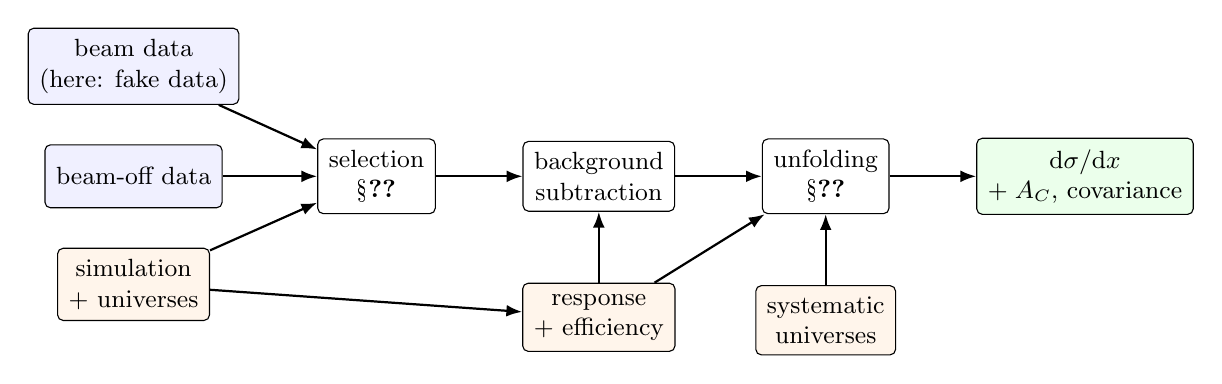
\begin{tikzpicture}[
      font=\small,
      box/.style={draw, rounded corners=2pt, align=center, inner sep=4pt, minimum height=8mm},
      data/.style={box, fill=blue!6},
      mc/.style={box, fill=orange!8},
      res/.style={box, fill=green!8},
      ar/.style={-{Latex[length=2mm]}, thick}]
    \node[data] (d) {beam data\\(here: fake data)};
    \node[data, below=5mm of d] (ext) {beam-off data};
    \node[mc, below=5mm of ext] (mc) {simulation\\$+$ universes};
    \node[box, right=12mm of ext] (sel) {selection\\\S\ref{sec:selection}};
    \node[box, right=11mm of sel] (sub) {background\\subtraction};
    \node[box, right=11mm of sub] (unf) {unfolding\\\S\ref{sec:unfolding}};
    \node[res, right=11mm of unf] (xs) {$\mathrm{d}\sigma/\mathrm{d}x$\\$+\;A_C$, covariance};
    \node[mc, below=9mm of sub] (resp) {response\\$+$ efficiency};
    \node[mc, below=9mm of unf] (cov) {systematic\\universes};
    \draw[ar] (d) -- (sel); \draw[ar] (ext) -- (sel); \draw[ar] (mc) -- (sel);
    \draw[ar] (sel) -- (sub); \draw[ar] (sub) -- (unf); \draw[ar] (unf) -- (xs);
    \draw[ar] (resp) -- (sub); \draw[ar] (resp) -- (unf); \draw[ar] (cov) -- (unf);
    \draw[ar] (mc) -- (resp);
  \end{tikzpicture}
  \caption{The extraction chain. The same selection is applied to data, beam-off data and
    simulation; the simulation additionally supplies the response and the systematic universes. What
    comes out is a cross section together with the additional-smearing matrix $A_C$ and the
    covariance --- all three are needed to compare it with a prediction.}
  \label{fig:chain}
\end{figure}

\subsection*{How to read this note}

\S\ref{sec:results} is the results section and can be read on its own; \S\ref{sec:wtki} gives the
proton-tagged subsample, which is secondary scope. Terms of art --- smearceptance, $A_C$, universe, closure, conditioning and the rest --- are
defined in plain language in the Glossary at the end, in the order a reader meets them. Two
companion documents carry material that would otherwise interrupt the argument: the \emph{technical supplement} holds the studies behind
the analysis choices --- estimator surveys, binning and threshold optimisation, the closure
programme, the control-region procedure --- and the \emph{change log} holds the history of the
analysis, including every correction that changed a result and the values before and after. Neither
is needed to follow this note. The additional-smearing and covariance matrices for every extraction
are released as text in \texttt{report/data\_release/}; a prediction cannot be compared with these
results without the former, nor used quantitatively without the latter.

% =============================================================================
\section{Analysis status}
\label{sec:status}
% =============================================================================

This section is the one-page version of the analysis, and the status of everything in it.

\paragraph{What is measured.} Flux-averaged $\nu_\mu+\bar\nu_\mu$ charged-current
single-charged-pion production on argon. The signal is defined by what leaves the nucleus --- one
muon, one charged pion, no neutral pion, any number of nucleons, vertex in the fiducial volume ---
not by the interaction mechanism, in the phase space $p_\mu>0.15$~GeV/$c$, $p_\pi>0.175$~GeV/$c$
and $\theta_{\mu\pi}<2.6$~rad.

\paragraph{From what.} The full NuMI exposure: FHC $8.857\times10^{20}$~POT, RHC
$11.082\times10^{20}$, combined $19.939\times10^{20}$, each normalised run by run and each with its
own integrated flux. The selection reaches $\approx\!17\%$ efficiency at $\approx\!59\%$ purity; the
dominant background is CC$0\pi$ with a proton taken for the pion, then multi-pion events, with
beam-off cosmics at $\approx\!2\%$ of the prediction.

\paragraph{What comes out.} A flux-averaged total from a one-bin extraction, six differential
distributions, and a proton-tagged subsample measured as secondary scope;
Table~\ref{tab:inventory} is the full inventory. All angles are defined about the neutrino
direction, not the detector axis --- using the detector axis would move about $65\%$ of signal
events to a different $\cos\theta_\mu$ bin.

\paragraph{How to compare a prediction with it.} Multiply the prediction by the released
additional-smearing matrix $A_C$, then use the released covariance. $A_C$ is not
normalisation-preserving, so the integral of a differential result is not the total cross section
and differs between observables; the physical total is the one-bin extraction, where $A_C=1$.

\begin{center}
\fbox{\begin{minipage}{0.94\textwidth}
\textbf{Status of every product}
\begin{itemize}\itemsep1pt \setlength{\parskip}{0pt}
  \item \textbf{Signal region: blinded.} Every data point in this note is a Poisson throw of the
    central-value simulation. No statement here is a measurement of beam-on data.
  \item \textbf{Control regions: opened} on beam-on data under the frozen procedure; they indicate
    no correction to the background-class normalisations (\S\ref{sec:cr_outcome}).
  \item \textbf{Primary:} the inclusive one-bin total and the six inclusive differential
    distributions, in all three configurations.
  \item \textbf{Secondary:} the proton-tagged one-bin total. The proton-tagged differential
    observables are carried as validation products and are not proposed for approval in this review.
  \item \textbf{Proposed:} the proton angles $\theta_p$ and $\theta_{\pi p}$, and two
    two-dimensional pairs in the combined configuration only.
  \item \textbf{Withdrawn --- do not quote:} the differential $W_{\pi p}$ shape and the five-bin
    $d\sigma/dp_\pi$ (Appendix~\ref{app:withdrawn}).
  \item \textbf{Validated:} the implementation, the size of the statistical uncertainties, and
    robustness to a materially different interaction model --- no bin biased by more than
    $0.8\sigma$, though the two edge bins move by $30$--$60\%$ (\S\ref{sec:altmodel}). Not yet
    extended to RHC or the proton-tagged family.
  \item \textbf{Uncertainties:} the nominal configured covariance. Identified terms that are
    \emph{not} in it are listed in \S\ref{sec:limitations}.
  \item \textbf{Before the signal region is opened:} the FHC Run-1 exposure must be resolved --- the
    beam-on sample appears to be the one recorded without the open trigger, which would raise the
    FHC cross section by $14\%$ --- and the flux normalisation must be confirmed with the flux
    contact.
\end{itemize}
\end{minipage}}
\end{center}

% =============================================================================
\section{Physics Context}
\label{sec:theory}
% =============================================================================

\subsection{Production mechanisms and nuclear effects}
\label{sec:prod_mechanisms}
\label{sec:fsi}

At $0.5$--$5$~GeV charged-current single charged-pion production proceeds through baryon
resonance production, dominated by the $\Delta(1232)$ and modelled by Rein--Sehgal-type
form factors~\cite{rs1981,kuzmin2004,graczyk2008,berger2007,nowak2009}; a non-resonant
continuum and deep-inelastic scattering, together $\sim\!20\%$ of the rate here and added
incoherently by every generator used; and coherent production off the whole nucleus
($\lesssim10\%$), which satisfies the topological signal definition of \S\ref{sec:signal}
and is therefore part of the signal, not a background. On argon, Fermi motion, Pauli
blocking and binding modify the kinematics, and final-state interactions (absorption at
$\sim\!25$--$30\%$, charge exchange, quasi-elastic scattering) mix the CC$\pi^{\pm}$,
CC$\pi^0$ and CC$0\pi$ topologies at the $30\%$ level. That mixing is why the signal is
defined by the final-state particle content and not by the production process, and why
CC$0\pi$ is the largest background: pion absorption and a proton taken for the pion feed
it into the selection (\suppref{Sec.}{sec:request}).

\subsection{Generators compared}
\label{sec:generators}

Four generators are compared with the results; their relevant model choices are
summarised in Table~\ref{tab:gen_config}. The injected model and the source of the
response is the \uboone{} tune of GENIE~v3~\cite{uboone_tune}. In the measured phase
space the standalone generators span a factor of $\sim\!1.6$ in the total cross section,
GENIE lowest and NEUT highest (\suppref{Table}{tab:total_xsec}), bracketing the tune;
because the present results are extracted on central-value fake data, that spread is the
context for the model comparisons, not a measured tension.

\begin{table}[H]
  \centering
  \caption{Model content of the generators compared, restricted to what matters for
    interpreting this measurement.}
  \label{tab:gen_config}
  \small
  \begin{tabular}{L{2.0cm} L{4.6cm} L{3.4cm} L{4.2cm}}
    \toprule
    Generator & Resonance model & Non-resonant / DIS & Final-state interactions \\
    \midrule
    GENIE v3~\cite{genie,genie3} & KLN--BS, 18 resonances to $W\lesssim2$~GeV & Bodek--Yang, incoherent; AGKY transition & INTRANUKE hA (one effective interaction) \\
    NuWro~\cite{nuwro} & $\Delta(1232)$ only (Paschos--Yu) & separate amplitude; smooth transition to Bodek--Yang & Salcedo--Oset (in-medium $\Delta$, two-body absorption) \\
    NEUT~\cite{neut,neut2021} & modified Rein--Sehgal, 18 resonances, Graczyk--Sobczyk $\Delta$ form factors & GRV98 with Bodek--Yang above $W\approx2$~GeV & step-by-step intranuclear cascade \\
    GiBUU~\cite{gibuu} & $\Delta$ and higher resonances with in-medium spectral functions & PYTHIA fragmentation above $W\approx1.6$~GeV & transport equations with pion optical potential \\
    \bottomrule
  \end{tabular}
\end{table}

\subsection{Previous measurements}
\label{sec:prev_meas}

Table~\ref{tab:prev_meas} lists the published CC$\pi^+$ measurements on nuclear targets.
The two most directly relevant are MicroBooNE's own: the BNB
measurement~\cite{uboone_bnb2026_ccpi}, on the same detector with an on-axis spectrum
peaked at $0.7$~GeV and negligible $\bar\nu_\mu$ content, gives
$\sigma=(3.75\pm0.07_{\rm stat}\pm0.80_{\rm syst})\times10^{-38}$~cm$^2$/Ar and finds
all tested generators above the data at very forward muon angles; and the NuMI
$\nu_e+\bar\nu_e$ CC$\pi^+$ measurement~\cite{uboone_nue_ccpi}, on the same beam and
reconstruction, which shares this analysis's extraction framework and conventions
(\suppref{Sec.}{sec:nueconsistency}). The NuMI off-axis flux used here is softer and
broader than the BNB one with a $\sim\!35\%$ $\bar\nu_\mu$ admixture in FHC, and the
flux-averaged total is divided by the whole flux above $60$~MeV while pion production
opens near $0.3$~GeV, so the $\sim\!1.0\times10^{-38}$~cm$^2$/Ar found here is not to be
compared directly with the BNB value (\S\ref{sec:flux_status}). The T2K off-axis
measurement on carbon~\cite{t2k_ccpip} overlaps this spectrum most closely among the
other experiments. The extended survey is in the technical supplement
(\suppref{App.}{sec:supp_physics}).

\begin{table}[H]
  \centering
  \caption{Selected CC$\pi^+$ cross-section measurements on nuclear targets.
    $\langle E_\nu\rangle$ is the approximate mean or peak neutrino energy.
    ``Type'' indicates whether a total integrated (T) or differential (D)
    cross section was reported.  ``Target'' gives the nucleus primarily used for
    cross-section extraction.}
  \label{tab:prev_meas}
  \small
  \begin{tabular}{L{2.1cm} L{1.4cm} C{1.4cm} C{0.8cm} L{4.8cm}}
    \toprule
    Experiment & Target & $\langle E_\nu\rangle$ (GeV) & Type & Key result / reference \\
    \midrule
    ANL 12-ft~\cite{anl_radecky1982}     & D         & 1.0   & T & Bubble chamber; foundational $\sigma$ vs $E_\nu$ \\
    BNL 7-ft~\cite{bnl_kitagaki1986}     & D         & 1.5   & T & Higher statistics; 15\% normalisation tension with ANL \\
    K2K~\cite{k2k_rodriguez2008}         & C         & 1.3   & T & First accelerator CC$\pi^+$ on carbon near detector \\
    MiniBooNE~\cite{miniboone_ccpi}      & CH$_2$    & 0.7   & D & $Q^2$, $W$, $p_\mu$, $\theta_\mu$; 20\% excess over NUANCE \\
    MINERvA~\cite{minerva_ccpi}          & CH        & 3.6   & D & $p_\pi$, $\theta_\pi$, Adler angles; NuMI medium-energy \\
    T2K ND280~\cite{t2k_ccpip}          & CH        & 0.85  & D & $p_\mu$, $\cos\theta_\mu$; off-axis beam similar to this work \\
    ArgoNEUT~\cite{argoneut_ccpi}        & Ar        & 9.6   & T & First CC$\pi^+$ on Ar; 115~$\nu$ + 158~$\bar\nu$ events (1.25$\times$10$^{20}$~POT) \\
    \uboone{} BNB~\cite{uboone_bnb2026_ccpi}       & Ar        & 0.7   & D & Full BNB dataset (1.11$\times$10$^{21}$~POT); $\sigma=(3.75\pm0.80)\times10^{-38}$~cm$^2$/Ar \\
    \uboone{} NuMI $\nu_e$~\cite{uboone_nue_ccpi} & Ar & 0.73 & D & First $\nu_e+\bar\nu_e$ CC$\pi^+$ on Ar; $\sigma=(0.93\pm0.28)\times10^{-39}$~cm$^2$/nucleon \\
    \bottomrule
  \end{tabular}
\end{table}

% =============================================================================

\section{Beam and Neutrino Flux}
\label{sec:flux}
% =============================================================================

\subsection{NuMI beam and flux composition}

The NuMI beam is produced by 120~GeV protons from the Fermilab Main Injector
striking a graphite target. Charged secondary hadrons are focused by two magnetic
horns whose polarity selects the sign of the focused mesons. In Forward Horn
Current (FHC) mode the horns focus positive pions and kaons, giving a beam with
predominantly $\nu_\mu$ content; in Reverse Horn Current (RHC) mode the polarity
is reversed to focus negatives, giving a predominantly $\bar{\nu}_\mu$ beam.
\uboone{} is located $135$~mrad ($7.71^\circ$) off-axis from the NuMI beam axis\footnote{From the detector position in beam coordinates, $(5502,\,7259,\,67270)$~cm: $91.1$~m transverse at $672.7$~m downstream. Earlier versions of this note quoted $110$~mrad. See \S\ref{sec:beamdir}.},
reducing the peak neutrino energy to the 0.5--2.5~GeV range and narrowing the
energy spectrum. Because \uboone{} sits off-axis and at comparatively low energy,
the horn sign-selection is imperfect and both modes carry a sizeable wrong-sign
component, most notably RHC, whose wrong-sign $\nu_\mu$ fraction is large.

The flux composition at the \uboone{} site is taken from the new-G4 central-value
flux histograms, integrated over $E_\nu > 60$~MeV to
exclude an unphysical sub-threshold pile-up near $E_\nu = 0$ (removed by the
flux group's low-energy peak removal; below the reaction threshold and
irrelevant to the measurement). The muon-flavour split of these central-value
histograms matches the author's authoritative integrated fluxes exactly
(Sec.~\ref{sec:flux_status}):

\begin{table}[H]
  \centering
  \caption{NuMI flux composition at the \uboone{} site by neutrino type, for the FHC
    and RHC horn modes (new-G4 central-value flux,
    integrated over $E_\nu>60$~MeV, the same threshold as the authoritative integrals of
    Table~\ref{tab:flux}; above $0.1$~GeV the RHC split would read $42.0/55.2\%$). FHC is $\nu_\mu$-dominant; RHC is
    $\bar{\nu}_\mu$-dominant with a large wrong-sign $\nu_\mu$ fraction. The combined
    row weights each mode by its fluence, $\Phi\times$POT (FHC $6.03$, RHC
    $7.14\times10^{11}$~cm$^{-2}$; Tables~\ref{tab:pot} and~\ref{tab:flux}), giving a near-balanced
    $\nu_\mu/\bar{\nu}_\mu$ mix. The signal is charge-blind ($|\nu_\mathrm{pdg}|=14$),
    so both $\nu_\mu$ and $\bar{\nu}_\mu$ contribute in every mode.}
  \label{tab:fluxcomp}
  \begin{tabular}{lcccc}
    \toprule
    Horn mode & $\nu_\mu$ & $\bar{\nu}_\mu$ & $\nu_e$ & $\bar{\nu}_e$ \\
    \midrule
    FHC & $63.4\%$ & $34.0\%$ & $1.7\%$ & $0.9\%$ \\
    RHC & $44.2\%$ & $53.3\%$ & $1.4\%$ & $1.2\%$ \\
    Combined & $53.0\%$ & $44.4\%$ & $1.5\%$ & $1.1\%$ \\
    \bottomrule
  \end{tabular}
\end{table}

Flux corrections from the Package to Predict the FluX (PPFX)~\cite{ppfx} are
applied per event via the central-value weight stored in the
analysis ntuples. The absolute flux normalisation of Sec.~\ref{sec:flux_status} uses
the same new-G4 histograms.

\subsection{Beam direction in detector coordinates}
\label{sec:beamdir}

Two different angles describe the \uboone{}--NuMI geometry, and they must not be
confused (Fig.~\ref{fig:numigeom}). The \emph{off-axis angle} is a property of the
beamline: the detector sits $91.1$~m off the NuMI axis at $672.7$~m downstream of the
target, a baseline of $678.8$~m and an off-axis angle of $7.71^\circ$
($134.6$~mrad).\footnote{Computed from the detector position in beam coordinates,
$(5502,\,7259,\,67270)$~cm, taken from the same rotation matrix used for the NuMI
beamline geometry weights.} That angle says nothing about how the TPC is oriented.

The angle that enters the measurement is a different one: the direction in which the
neutrinos travel \emph{relative to the detector $z$ axis}. Averaged over interactions
in the active volume, the true neutrino direction in detector coordinates is
$(0.4624,\,0.0489,\,0.8853)$, which lies $28.6^\circ$ away from $z$. The detector $z$
axis is therefore a poor measurement coordinate for the beam: it is not the direction the neutrinos
came from, nor the NuMI beamline axis (itself $23.2^\circ$ from $z$).

\begin{figure}[H]
  \centering
  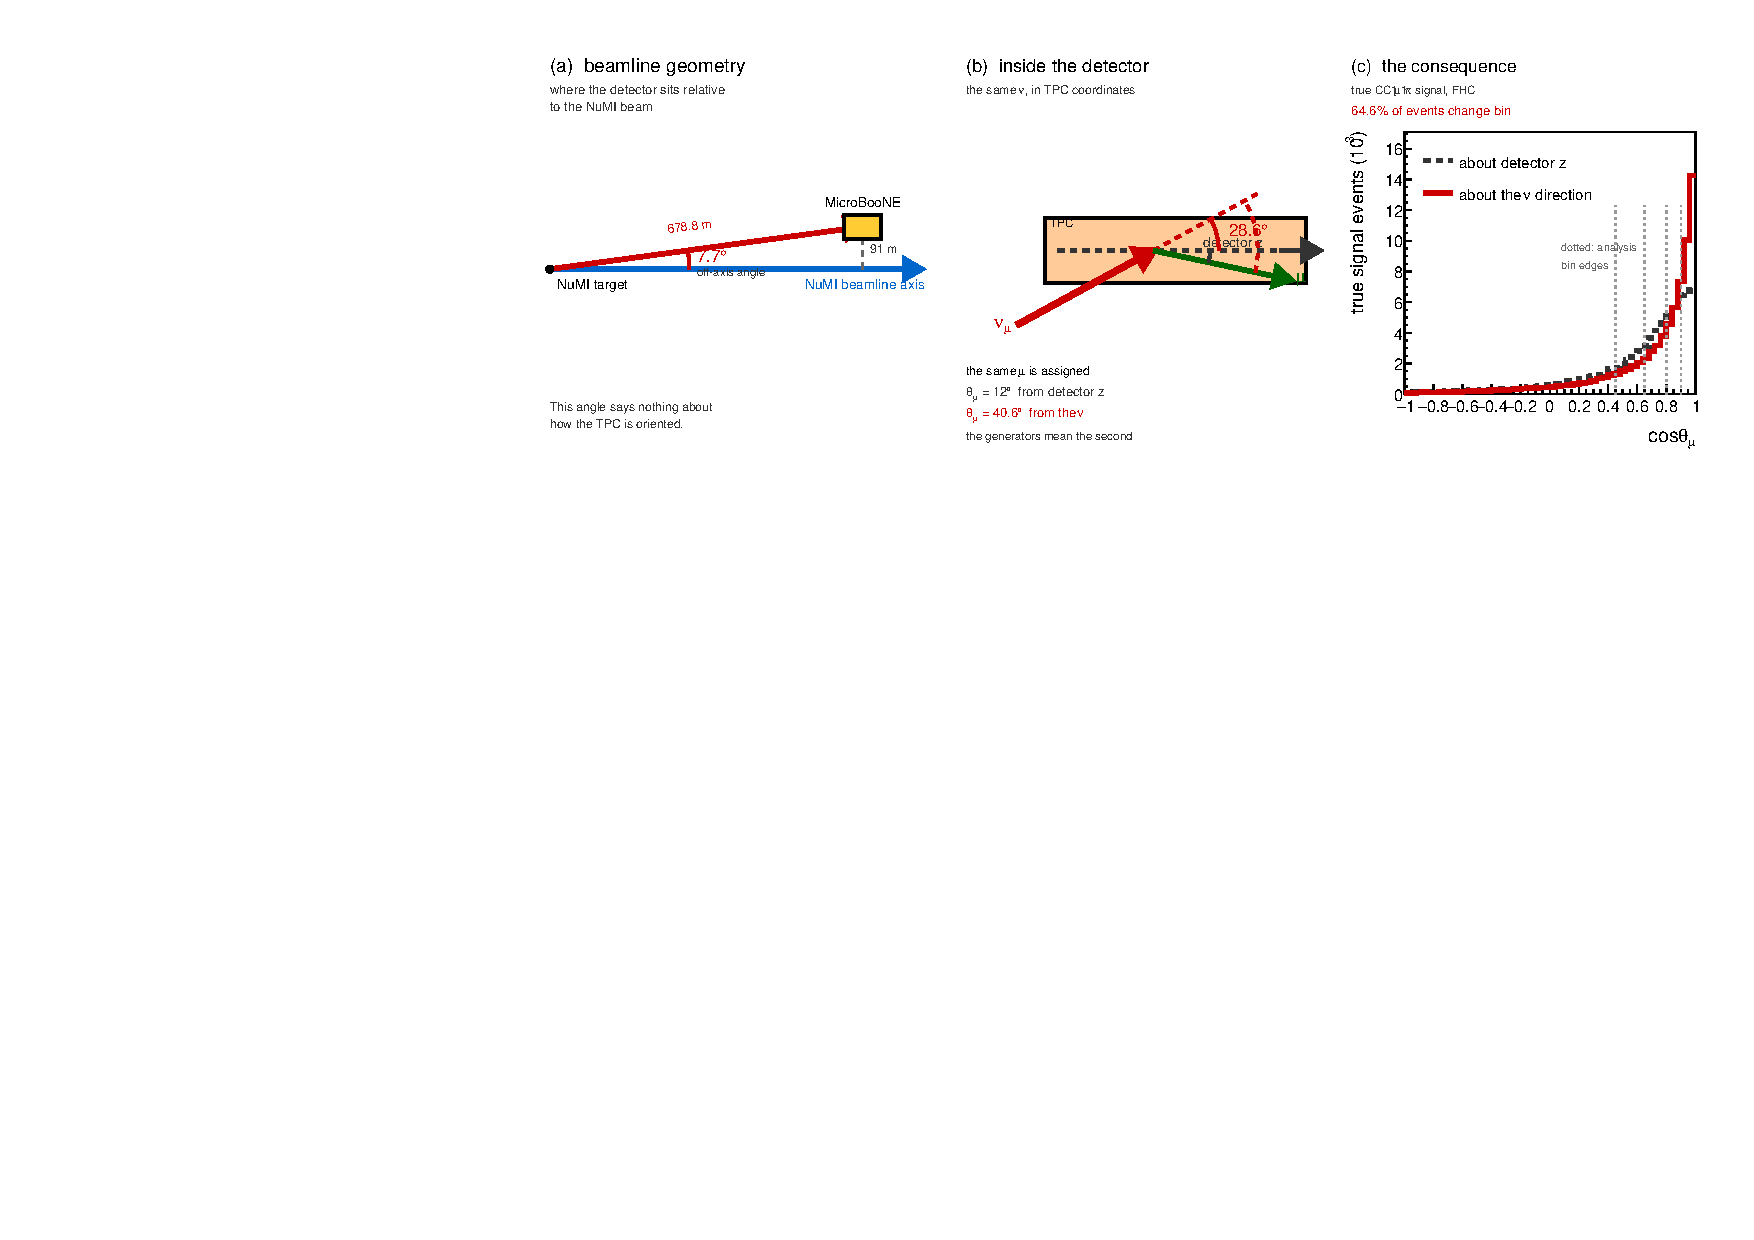
\includegraphics[width=\textwidth]{numi_geometry}
  \caption{The NuMI geometry seen by \uboone{}. (a) Beamline geometry, to scale: the
    detector sits $91.1$~m off the NuMI axis at a baseline of $678.8$~m, an off-axis
    angle of $7.7^\circ$. (b) The same neutrinos in TPC coordinates, to scale (the
    $x$--$z$ projection; the quoted $28.6^\circ$ is the full three-dimensional angle):
    the beam arrives $28.6^\circ$ away from the detector $z$ axis, so one and the same
    muon is assigned $\theta_\mu=12^\circ$ about $z$ but $\theta_\mu=40.6^\circ$ about
    the neutrino. The generators mean the second. (c) The resulting shift in the true
    $\cos\theta_\mu$ distribution; dotted lines mark the analysis bin edges. Under the
    two conventions $64.6\%$ of signal events fall in a different bin ($44.6\%$ for
    $\cos\theta_\pi$).}
  \label{fig:numigeom}
\end{figure}

This matters because every polar angle and every transverse-kinematic-imbalance
variable is defined with respect to the neutrino direction. In the generator
predictions the neutrino defines $+z$ by construction --- the GENIE event records used
here have $p_x^\nu=p_y^\nu=0$ and $p_z^\nu=E_\nu$ exactly --- so a measurement that
refers its angles to the detector $z$ axis is not being compared with the prediction
it appears to be compared with. The effect is not small: $64.6\%$ of signal events
change $\cos\theta_\mu$ bin between the two conventions, and $44.6\%$ change
$\cos\theta_\pi$ bin. For the TKI variables the axis error exceeds the observable
itself, the mean $\delta p_T$ being $0.742$~GeV/$c$ about $z$ against $0.264$~GeV/$c$
about the beam.

Accordingly, all angular and TKI observables in this analysis are referred to the
neutrino direction, following the $\beta$ convention of the NuMI $\nu_e$ CC$1\pi$
internal note~\cite{numi_nue_ccpi} and of the earlier NuMI $\nu_e$ cross-section
measurement it derives from~\cite{mistry_thesis}. At truth level the exact per-event
neutrino direction is used, which reproduces the generator convention exactly. At
reconstruction level the neutrino direction is approximated by the vector from the
NuMI target --- at $(-31388,\,-3316,\,-60100)$~cm in detector coordinates, a $684$~m
baseline to the detector centre ($678.8$~m to the TPC origin quoted above) --- to the
reconstructed interaction vertex. Adopting the same $\beta$ as the
$\nu_e$ analysis keeps the two NuMI measurements directly comparable.

The choice of reconstruction-level axis is in any case not a sensitive one. A single
fixed axis and the per-event $\beta$ differ by a median of $2.4$~mrad (maximum
$7.3$~mrad), which moves only $0.42\%$ of muons across a $\cos\theta_\mu$ bin edge ---
to be compared with the $64.6\%$ moved by the detector-$z$ convention. Against the true
per-event direction the two perform almost identically, with a mean opening angle of
$1.95^\circ$ for $\beta$ and $2.00^\circ$ for a fixed axis. What neither can recover is
the physical divergence of the beam: neutrinos reaching the detector come from decays
distributed along the decay pipe, not from the target, and over a $684$~m baseline a
$2.5$~m detector subtends only ${\sim}4$~mrad, so the vertex position carries almost no
information about the direction. That residual is a resolution effect, absorbed by the
response matrix like any other.

Quantities that are invariant under this choice of axis are unaffected: $p_\mu$,
$p_\pi$, the muon--pion opening angle $\theta_{\mu\pi}$, the invariant mass
$W_{\pi p}$, and all integrated cross sections. The event selection is likewise
unaffected, as no selection cut and no BDT input variable uses a polar angle.

\subsection{Data exposure}

The analysis is \emph{blind}: the real beam-on data are not used. Each configuration
is extracted on Poisson-thrown central-value fake data, generated and scaled
\emph{per run} to that run's data POT (Table~\ref{tab:pot}). The FHC measurement uses
the full FHC exposure (Runs~1, 2, 4 and~5); RHC uses Runs~1, 2, 3, 4a, 4b and~4c; the
combined measurement uses all fourteen overlay files. Every run is normalised
independently to its own data exposure, so the prediction carries the data-POT mixture
of run periods and the framework is ready for real per-run beam-on data (each fake-data
sample is a drop-in replacement for its beam-on counterpart).

\begin{table}[H]
  \centering
  \caption{Run-period exposure accounting (final, full FHC$+$RHC). ``MC POT'' is each
    period's native simulated exposure; ``Data POT'' is the per-run exposure to which
    the (blind, per-run) fake data is scaled. \emph{Each run is normalised
    independently} by its own factor, Scale $=$ (run Data POT)$/$(run MC POT), so the
    prediction is the data-POT--weighted mixture of run periods; the normalisation a
    real per-run beam-on dataset produces. This replaces an earlier single per-mode
    pooling factor: because the per-run MC/data POT ratios vary by up to a factor of
    three (Scale ranges $0.051$--$0.141$ within FHC alone), a single factor would weight
    the runs by their MC statistics rather than by the data exposure. The RHC Run~4 row
    sums the 4a/4b/4c sub-files and Run~3 sums aa--ae; sub-files sharing a run's data POT
    are scaled by the group MC total so they pool within that run. The combined
    measurement applies each run's own factor. Run~5 uses the $\nu_\mu$ overlay produced
    with reweighted PPFX flux weights (the only Run-5 overlay available). The fake data are
    thrown from the same per-run-scaled prediction, so the closure (Table~\ref{tab:fhc})
    tests the bookkeeping of this scheme, not its correctness against data.}
  \label{tab:pot}
  \begin{tabular}{lccc}
    \toprule
    Run period & MC POT ($\times10^{20}$) & Data POT ($\times10^{20}$) & Scale \\
    \midrule
    Run~1 (FHC)  & 23.282 &  3.283 & 0.1410 \\
    Run~2 (FHC)  & 24.934 &  1.268 & 0.0509 \\
    Run~4 (FHC)  & 28.335 &  2.075 & 0.0732 \\
    Run~5 (FHC)  & 19.300 &  2.231 & 0.1156 \\
    \textbf{FHC total} & \textbf{95.85} & \textbf{8.857} & \emph{per run} \\
    \midrule
    Run~1 (RHC)      &  8.997 & 0.605 & 0.0673 \\
    Run~2 (RHC)      & 57.865 & 2.591 & 0.0448 \\
    Run~3 (RHC, aa--ae) & 55.185 & 5.003 & 0.0907 \\
    Run~4 (RHC, 4a--4c) & 32.586 & 2.883 & 0.0885 \\
    \textbf{RHC total} & \textbf{154.63} & \textbf{11.082} & \emph{per run} \\
    \midrule
    \textbf{Combined (FHC$+$RHC)} & \textbf{250.49} & \textbf{19.939} & \emph{per run} \\
    \bottomrule
  \end{tabular}
\end{table}

The full exposure substantially reduces the data-statistical term
(\suppref{Table}{tab:systbreak_fhc}--\suppref{Table}{tab:systbreak_comb}), leaving the
measurement flux- and detector-systematic limited. When the analysis is
unblinded, the real beam-on POT (and gate counts) replace the data-POT values
above.

\subsection{Integrated flux}
\label{sec:flux_status}

The absolute flux normalisation uses the new-G4 GEANT4 NuMI flux
integrated over $E_\nu > 60$~MeV (the flux group's
low-energy peak removal, which removes an unphysical $\sim$25--30~MeV artifact
spike). The signal is charge-blind ($|\nu_\mathrm{pdg}| = 14$, covering both
$\nu_\mu \to \mu^-\pi^+$ and $\bar{\nu}_\mu \to \mu^+\pi^-$), so the normalisation
uses the combined $\nu_\mu + \bar{\nu}_\mu$ flux $\Phi = \Phi_{\nu_\mu} +
\Phi_{\bar{\nu}_\mu}$. Because RHC is $\bar{\nu}_\mu$-dominant with a different
absolute flux than FHC, each configuration uses its \emph{own} integrated flux:

\begin{table}[H]
  \centering
  \caption{Integrated $\nu_\mu$ and $\bar{\nu}_\mu$ fluxes per POT used by the analysis
    (new-G4 flux, $E_\nu > 60$~MeV), and the combined $\nu_\mu+\bar{\nu}_\mu$ value
    used as the per-configuration normalisation. The combined row is the
    data-POT-weighted average of the two modes (weights $8.857 : 11.082$;
    Table~\ref{tab:pot}). Each configuration is normalised with its own flux: the RHC
    flux is $5.4\%$ below the FHC one, so using a single value for both would bias the
    RHC cross section by that amount.}
  \label{tab:flux}
  \begin{tabular}{lcccc}
    \toprule
    Config & $\Phi_{\nu_\mu}$ & $\Phi_{\bar{\nu}_\mu}$ & $\Phi_{\nu_\mu+\bar{\nu}_\mu}$ & $\bar{\nu}_\mu$ frac. \\
           & \multicolumn{3}{c}{($10^{-10}\,\mathrm{cm}^{-2}\,\mathrm{POT}^{-1}$)} & \\
    \midrule
    FHC      & $4.43515$ & $2.37644$ & $6.81159$ & $34.9\%$ \\
    RHC      & $2.92348$ & $3.52298$ & $6.44646$ & $54.6\%$ \\
    Combined & $3.59497$ & $3.01368$ & $6.60865$ & $45.6\%$ \\
    \bottomrule
  \end{tabular}
\end{table}

The mean energy of the $\nu_\mu+\bar\nu_\mu$ flux above $60$~MeV is $0.479$~GeV (FHC)
and $0.475$~GeV (RHC) ($\nu_\mu$ alone $0.468$ and $0.544$~GeV; $\bar{\nu}_\mu$ alone
$0.500$ and $0.417$~GeV, the RHC antineutrinos being the focused, softer component at
this off-axis angle). Only $40\%$ of that flux lies above $0.3$~GeV, $26\%$ above
$0.5$~GeV and $13\%$ above $1$~GeV. Because the
flux-averaged cross section divides by the \emph{whole} flux above $60$~MeV while single
pion production only opens near $0.3$~GeV, the total is roughly a factor $2.5$ smaller
than it would be on the BNB spectrum peaked at $0.7$~GeV; this, together with the
measured phase space ($p_\pi>0.175$~GeV/$c$, $\theta_{\mu\pi}<2.6$~rad), is why the
$\sim\!1.0\times10^{-38}$~cm$^2$/Ar found here is not to be compared directly with the
$3.75\times10^{-38}$~cm$^2$/Ar of the BNB measurement of \S\ref{sec:prev_meas}. These fluxes
are set per configuration in the extraction. Because every simulated event carries
the PPFX central-value flux correction (\S\ref{sec:mc}; mean $0.944$ on
selected signal), the integrated flux that divides the event rate must be the
PPFX-corrected central value, not the raw GEANT4 flux; the central-value histograms of the new-G4 flux file are taken
to be that central value, 
and this should be confirmed
with the flux author before unblinding\todo{ask flux expert}, since a raw-G4 integral would put every absolute
cross section $\sim\!5$--$6\%$ low. \textbf{Open normalisation sign-off} (not required
for the control-region opening, required before the signal region is opened): written
confirmation by the NuMI flux contact that the integrated constants of
Table~\ref{tab:flux} are PPFX-corrected central values consistent with the per-event
PPFX central-value weighting. The integrated values were validated four independent
ways: standalone NuWro and GENIE event generation on the same flux, the flux author's
numbers, and a GENIE closure.

The number of argon target nuclei in the fiducial volume is computed from first
principles as
\begin{equation}
  N_{\mathrm{Ar}} = \frac{\rho_{\mathrm{LAr}} \cdot V_{\mathrm{FV}} \cdot N_A}{A_{\mathrm{Ar}}}
  = 8.710\times10^{29},
  \label{eq:nar}
\end{equation}
with $\rho_{\mathrm{LAr}}=1.3836$~g/cm$^3$, $A_{\mathrm{Ar}}=39.948$~g/mol and
$N_A=6.02214076\times10^{23}$~mol$^{-1}$. The fiducial box is
$10<x<246$, $-101<y<101$, $10<z<986$~cm ($4.6528\times10^{7}$~cm$^3$), from which the
$675.1<z<775.1$~cm dead region is subtracted, leaving
$V_{\mathrm{FV}}=4.1761\times10^{7}$~cm$^3$. Without that subtraction the same
expression would give $9.705\times10^{29}$. This is the value the code uses, computed
by the extraction from the fiducial box with the dead slab removed, and it is the value
entering the conversion factor
of \S\ref{sec:unfolding} and the one-bin total of \S\ref{sec:total_xsec}.
The per-configuration normalisation factor is $N_{\mathrm{norm}} =
\Phi_\mathrm{mode}\cdot N_{\mathrm{POT,mode}}\cdot N_{\mathrm{Ar}}$, evaluated with
each mode's flux and data POT (Table~\ref{tab:pot}).

% =============================================================================
\section{Monte Carlo Samples}
\label{sec:mc}
% =============================================================================

Monte Carlo events are generated with GENIE~v3~\cite{genie,genie3} (the \uboone{}
tune~\cite{uboone_tune}) on argon-40, propagated through the detector with
Geant4~\cite{geant4}, and
overlaid with real cosmic-ray data (the ``overlay'' technique) so that simulated
events experience in-situ detector noise and cosmogenic activity.
Table~\ref{tab:samples} summarises the input samples.

\begin{table}[H]
  \centering
  \caption{Input samples (final, full FHC$+$RHC). ``$n$'' is the number of overlay
    files; ``MC POT'' is the summed native simulated exposure ($\times10^{20}$). The
    blind Poisson-thrown fake data stands in for the (unused) beam-on data; the
    detector variations use the native Run-4 FHC and RHC samples. The per-file lists
    and POT/trigger values are in the configuration tables of the release.}
  \label{tab:samples}
  \small
  \begin{tabular}{@{}l l c r@{}}
    \toprule
    Sample & Composition & $n$ & MC POT \\
    \midrule
    $\nu_\mu$ overlay (FHC) & Runs 1, 2, 4 (pandora) $+$ Run 5 (reweighted-PPFX) & 4 & $95.85$ \\
    $\nu_\mu$ overlay (RHC) & Runs 1, 2, 3, 4a, 4b, 4c (pandora)                & 10 & $154.63$ \\
    Dirt MC (interactions outside the cryostat) & GENIE NuMI dirt overlays, per run (Run-1 file standing in for Run~2) & 7 & n/a \\
    EXT (beam-off)         & cosmic data, per run, horn-mode-independent        & 7 & n/a \\
    Detector variations    & Run-4 FHC $+$ Run-4 RHC, CV $+$ 8 knobs each       & 18 & n/a \\
    Fake data (blind)      & Poisson-thrown central value, per configuration    & n/a & n/a \\
    Beam-on data           & blinded, not used until unblinding              & n/a & n/a \\
    \bottomrule
  \end{tabular}
\end{table}

\paragraph{Event weights.}
Each MC event is weighted by
\begin{equation}
  w = \text{Scale}[\text{run}] \times w_{\mathrm{PPFX}} \times w_{\mathrm{tune}},
\end{equation}
where $\text{Scale}[\text{run}] = (\text{run Data POT})/(\text{run MC POT})$ is the
\emph{per-run} POT factor of Table~\ref{tab:pot}: each run period is scaled
independently to its own data exposure, so the prediction reproduces the data-POT
mixture of runs rather than the MC-statistics mixture (see the caption of
Table~\ref{tab:pot}). Operationally this is exactly what the framework does natively
each overlay file carries its run's data POT via a matching per-run beam-on
(here, per-run fake-data) sample, and is scaled by $\text{run\_bnb\_pot}$ divided by that run's MC exposure, taken as the
sum of the \emph{distinct} exposure values stored by the run's files (the run
total under both processed-file conventions; caption of Table~\ref{tab:sigint_all}).
$w_{\mathrm{PPFX}}$ is the PPFX central-value flux correction and $w_{\mathrm{tune}}$
is the GENIE/GEANT4 reweighting correction. One weight rule is used everywhere:
\begin{equation}
  w_{\mathrm{safe}} = \begin{cases} 1, & w\ \text{non-finite},\ w<0,\ \text{or}\ w>30,\\
  w, & \text{otherwise (a weight of exactly zero is kept)},\end{cases}
  \label{eq:safeweight}
\end{equation}
applied to the product $w=\text{Scale}\times w_{\mathrm{PPFX}}\times w_{\mathrm{tune}}$
(including the $0.65$ normalisation weight the dirt overlay carries, which scales its
generated exposure to the out-of-cryostat rate expected at the NuMI site). The universe construction, the
covariance, the unfolding inputs, the cut-flow histograms, the count-level tables, the
control-region yields, the transfer factors and the beam-on comparison at unblinding all
use Eq.~\eqref{eq:safeweight}; one rule everywhere is what makes count-level and
covariance-level numbers comparable to the per cent. At unblinding the per-run
fake-data samples are replaced by the corresponding per-run beam-on files (same runs,
same POT), so the normalisation is already correct.

\paragraph{EXT scaling.}
Beam-off data are cosmic-only, so a beam-off sample is matched to a beam-on run by
\emph{run period} alone, irrespective of the horn polarity it was recorded under. Each run
period uses the beam-off sample(s) taken in that period, scaled by that run's
beam-on/beam-off gate ratio (times the $0.98$ NuMI beam-occupancy factor); where a run
has several beam-off files the framework sums their gate counts and pools them:
\begin{equation}
  \text{EXT}_{\text{run}} = 0.98\;\frac{\text{bnb\_gates}[\text{run}]}
  {\sum_{\text{files}\in\text{run}}\text{ext\_gates}}\;\sum_{\text{files}\in\text{run}} N^{\text{sel}}_{\text{EXT}} .
\end{equation}
The gate counts per run are released with the results (\texttt{data\_release/ext\_gates.tsv}). No Run-2
beam-off sample exists and none will be produced, so the Run-1 sample, the nearest
pre-CRT period, stands in for Run~2 permanently, scaled by its own gate count. The same beam-off files serve the FHC and RHC beam-on runs of a given period,
and the combined configuration lists each (file, run) pair once. The selected beam-off
rate per $10^{6}$ gates is $1.75$ (Run~1), $0.43$ (Run~3b), $1.15$ (Run~4) and $0.52$
(Run~5): the pre-CRT Run-1 rate is $1.5$--$4$ times the CRT-era ones (the rates carry
$16$--$35\%$ Poisson uncertainties, from $8$, $14$, $40$ and $10$ raw selected beam-off
events), which is why period matching rather than a pooled sample is used. At the FHC final cut the beam-off
background is $30$ events ($23$ RHC, $53$ combined), $1.9\%$ of the selected sample.
Figure~\ref{fig:ext_perrun} shows the per-period rates, scale factors and resulting
yields; the machine-readable version is \texttt{data\_release/ext\_gates.tsv}, and the
normalisation manifest (\suppref{Sec.}{sec:pipeline}) checks that every (beam-off file, run) pair enters each configuration exactly once and that the gate counts are consistent.

\begin{figure}[H]
  \centering
  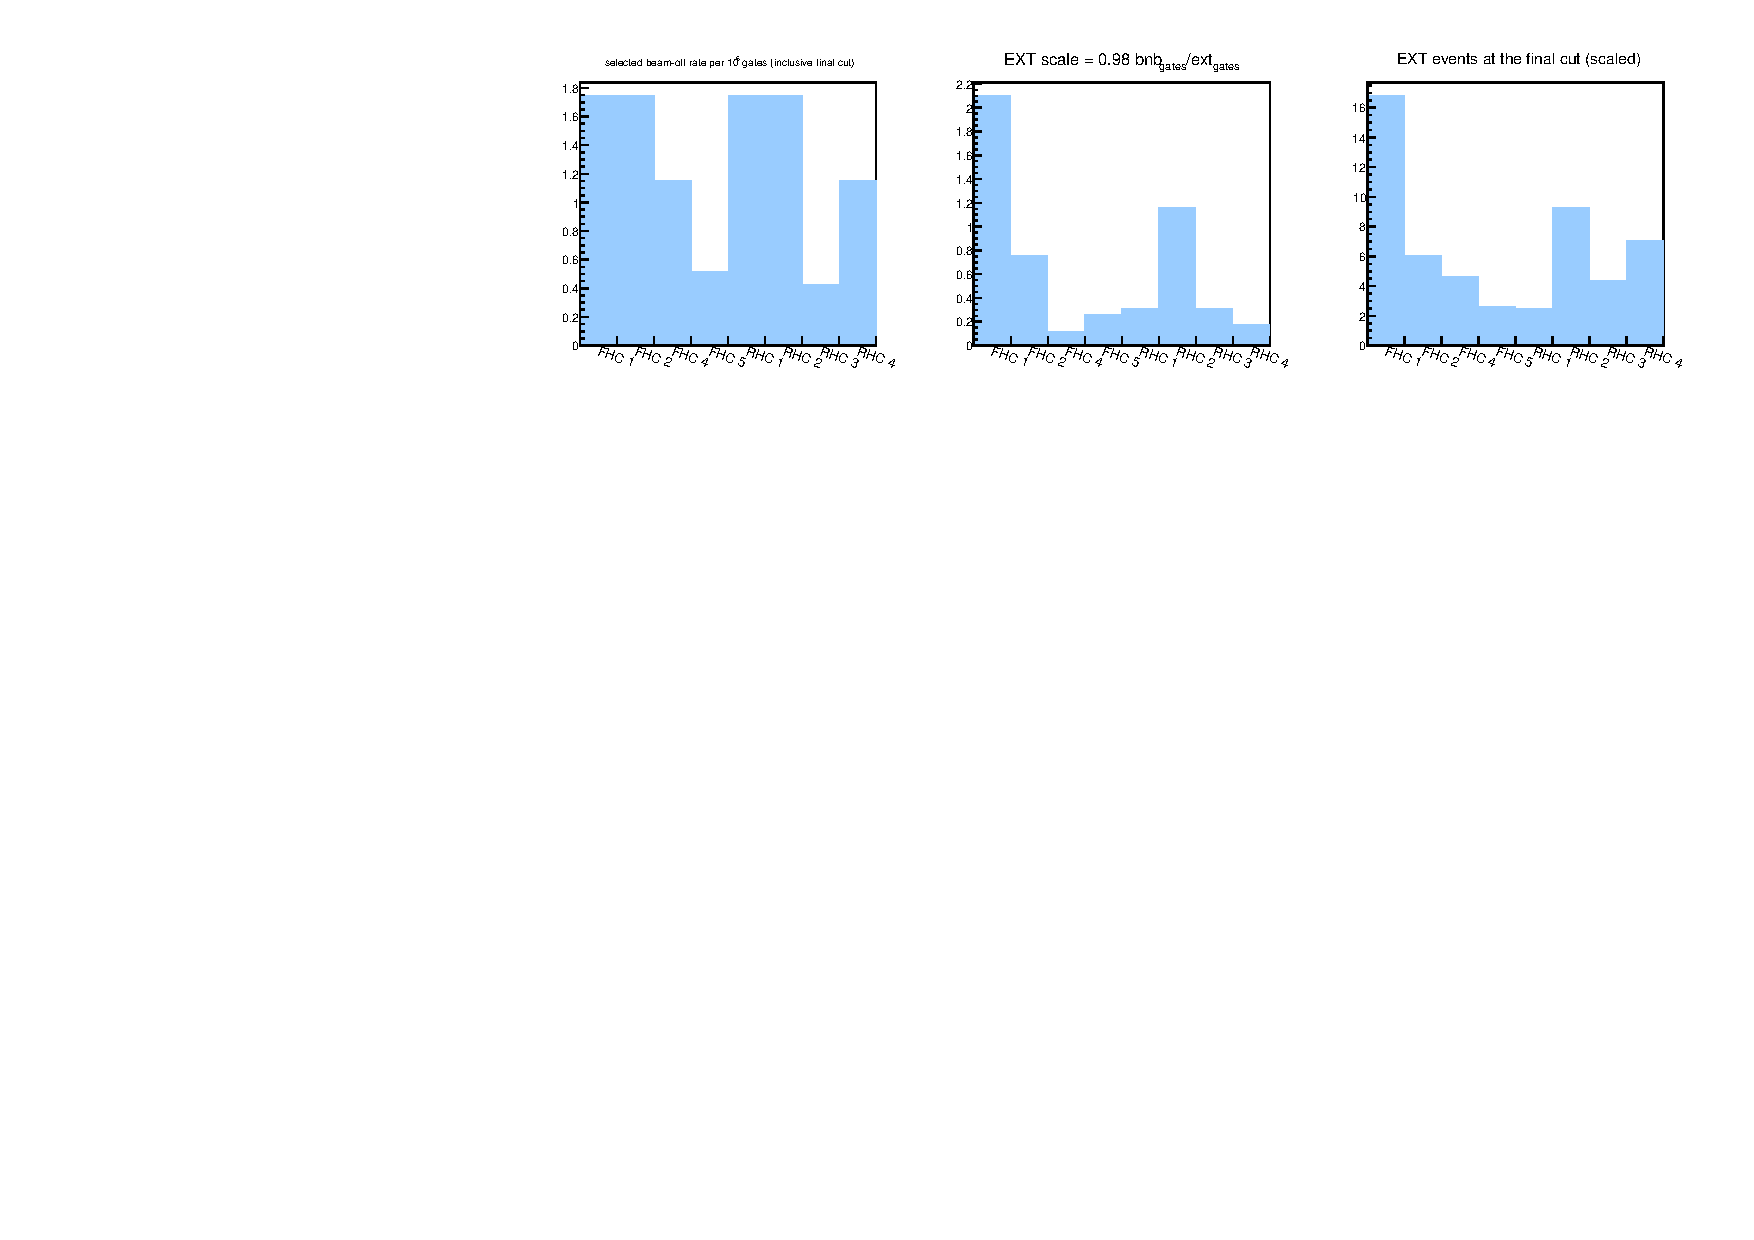
\includegraphics[width=\textwidth]{ext_perrun_validation}
  \caption{Beam-off validation by run period, from \texttt{data\_release/ext\_gates.tsv}:
    selected beam-off rate per $10^{6}$ gates at the inclusive final cut (left), the
    per-run scale factor $0.98\times$(beam-on gates)/(beam-off gates) (centre) and the
    resulting beam-off events at the final cut (right), for each beam-on run period of
    the FHC and RHC configurations. The Run-1 sample serves Run~2 of both modes as a
    stand-in (for RHC Run~1 it is the native period sample). The pre-CRT Run-1 rate is
    $1.5$ to $4$ times the CRT-era ones.}
  \label{fig:ext_perrun}
\end{figure}

\paragraph{No further cosmic-rejection cut.} Further cosmic-rejection cuts were not
adopted because the beam-off contribution is $1.9\%$ of the selected prediction and is
removed by an unbiased data-driven subtraction, so a cut can only reduce the
subtraction's statistical uncertainty, about six events on a sample of $1\,612$; every
plausible cut loses more signal than that. The directional and calorimetric variants
that were considered are in \suppref{Sec.}{sec:supp_cosmiccut}.

\paragraph{Software trigger.}
Data and EXT files are pre-filtered to require the software trigger; the CRT-era
beam-off files (Runs~4--5) carry a vestigial trigger flag that is zero throughout, so for
those files the pre-CRT trigger flag is used instead. MC events failing the software
trigger are
removed at the NeutrinoSlice cut stage.  In practice this has no measurable effect at the current
working point: all MC events passing the topological cut are verified to pass the
software trigger.

% =============================================================================
\section{Signal Definition}
\label{sec:signal}
% =============================================================================

The signal is defined at generator level and is used only to construct the
selection efficiency and response matrix.  It is \emph{never} applied as a
reconstruction cut.  The definition is \emph{charge-blind}: both
$\nu_\mu \to \mu^- \pi^+$ and $\bar{\nu}_\mu \to \mu^+ \pi^-$ are treated as
signal on the same footing.

\begin{description}[style=nextline]
  \item[Neutrino flavour]
    $|\nu~\mathrm{PDG}| = 14$ ($\nu_\mu$ or $\bar{\nu}_\mu$).
  \item[Interaction type]
    Charged-current.
  \item[True vertex]
    Inside the fiducial volume (Section~\ref{sec:fv}).
  \item[Primary multiplicity]
    Exactly one muon ($|\mathrm{PDG}| = 13$), exactly one charged pion
    ($|\mathrm{PDG}| = 211$) \emph{of any momentum} among the primary final-state
    particles of the interaction (a second charged pion below threshold makes the event
    background, not signal; pions from the decay of primary hyperons are not primaries
    and are not counted), zero neutral pions ($|\mathrm{PDG}| = 111$),
    zero kaons ($K^\pm$, $K^0$, $K_S$, $K_L$) and no other mesons.  Any number of
    protons (and neutrons) is allowed.
  \item[Kinematic thresholds]
    $p_\mu > 0.15\GeVc$, $p_\pi > 0.175\GeVc$, and $\theta_{\mu\pi} < 2.6$~rad.
    These define the \emph{measured phase space}, chosen from the efficiency
    turn-on curves (Section~\ref{sec:cutflow}).  The momentum efficiency turns on
    sharply at $\sim$0.15--0.20\GeVc (set by the 10~cm muon and 20~cm pion
    track-length cuts); below that it is only $\sim$1--3\% with a strongly
    model-dependent correction.  The opening-angle upper bound ($2.6$~rad) excludes
    the large-angle region, which is dominated by cosmic and dirt background
    ($\sim$7\% purity in the $\theta_{\mu\pi}>2.513$~rad bin).  No \emph{lower}
    opening-angle cut is applied: the small-angle region is high-purity
    ($\sim$58\%), so cutting it would only remove signal (it is low-efficiency but
    not low-purity).  The same cut is applied at reco level so the signal and
    selection acceptances match.  The first $p_\mu$/$p_\pi$ bins and the
    $\theta_{\mu\pi}$ upper edge start/end at these thresholds.
\end{description}

(Earlier iterations used $p_\mu, p_\pi > 0.1\GeVc$ with the full $0$--$\pi$ angle;
that left near-dead efficiency bins at low momentum and at the large-angle
extreme.  The phase space above raises the efficiency from $12.1\%$ to $15.6\%$ at
$\sim$55\% purity at the beam-off scaling then in use, see Section~\ref{sec:cutflow}.)

\paragraph{Pion threshold and the sibling $\nu_e$ measurement.}
The companion MicroBooNE NuMI $\nu_e\,\mathrm{CC}\,1\pi$ analysis defines its pion
signal by kinetic energy, $\mathrm{KE}_\pi>40$~MeV, equivalent to
$p_\pi>0.113\GeVc$. Our $p_\pi>0.175\GeVc$ ($\mathrm{KE}_\pi>84$~MeV) is
therefore a higher threshold. Lowering it toward the $\nu_e$ value is possible,
the signal definition is a truth-level choice and the unfolding maps reco to truth
but the pion momentum reconstruction (track range under the muon hypothesis,
mass-corrected) degrades rapidly below $0.175\GeVc$.  The table below is the
study that led to \emph{rejecting} a lower threshold; it is not part of the measurement.
The measured phase space is $p_\pi > 0.175\GeVc$ throughout this note, and no cross
section is reported below it:

\begin{center}\small
\captionof{table}{Pion momentum reconstruction versus true $p_\pi$ (correctly
  reconstructed signal pions). Below the $0.175\GeVc$ threshold the bias
  and resolution blow up and the reconstructed fraction halves.}
\label{tab:pithresh}
\begin{tabular}{lccc}
\toprule
True $p_\pi$ [\GeVc] & Bias $\langle(p^{\mathrm{reco}}-p^{\mathrm{true}})/p^{\mathrm{true}}\rangle$ & RMS resolution & Reco fraction \\
\midrule
$0.080$--$0.113$ & $+131\%$ & $73\%$ & $3.4\%$ \\
$0.113$--$0.150$ & $+66\%$  & $56\%$ & $3.4\%$ \\
$0.150$--$0.175$ & $+30\%$  & $51\%$ & $4.3\%$ \\
$\mathbf{0.175}$--$\mathbf{0.250}$ (threshold) & $\mathbf{-8\%}$ & $\mathbf{31\%}$ & $\mathbf{10.0\%}$ \\
$0.250$--$0.400$ & $-30\%$  & $21\%$ & $10.4\%$ \\
\bottomrule
\end{tabular}
\end{center}

\noindent At the threshold the resolution is $31\%$; in the $[0.113,0.175]\GeVc$
region it is $51$--$56\%$ with a $+30$--$66\%$ bias and only $\sim\!3$--$4\%$
reconstructability. Extending the measurement to the $\nu_e$ threshold would thus
add bins carrying large, strongly model-dependent unfolding systematics. For
consistency with the $\nu_e$ measurement the threshold could be lowered to
$0.113\GeVc$ with the $[0.113,0.175]\GeVc$ region kept in a single coarse bin to
contain those systematics, or both phase spaces reported; this is a
systematics-versus-cross-analysis-consistency trade rather than a reconstruction
limitation.

\paragraph{Why the threshold was not lowered.} Extending to the sibling $\nu_e$
threshold was investigated and rejected: the $[0.113,0.175]\GeVc$ region has $2.2\%$
selection efficiency and a strongly model-dependent reconstruction correction.  The study
is recorded in the technical supplement.  It is not part of this measurement, and no cross
section is reported below $p_\pi>0.175\GeVc$.

\section{Fiducial Volume}
\label{sec:fv}
% =============================================================================

The fiducial volume (FV) is:
\begin{equation}
  x \in [10.0,\;246.0]\cm, \quad
  y \in [-101.0,\;+101.0]\cm, \quad
  z \in [10.0,\;986.0]\cm,
\end{equation}
with the dead-wire region $z \in [675.1,\;775.1]\cm$ excluded.
The total FV volume is
\begin{align}
  V_{\mathrm{FV}} &= (246-10)\times 202 \times (976-100)\cm^3 \nonumber\\
                  &= 236 \times 202 \times 876\cm^3
                   \approx 4.17\times10^7\cm^3.
\end{align}

A wider \emph{containment} region (2~cm inset from the active-volume faces, except
the top face, which is inset by $10$~cm) is used to require that the pion candidate
track endpoint is contained:
\begin{equation}
  x \in [2.0,\;254.35]\cm,\quad
  y \in [-113.53,\;+107.47]\cm,\quad
  z \in [2.1,\;1034.9]\cm.
\end{equation}

\subsection{Which volume applies where}
\label{sec:fv_where}

Three distinct volumes appear above and it is worth stating plainly which is used for what,
since ``contained'' and ``in the fiducial volume'' are not the same requirement.

\begin{center}\small
\begin{tabular}{lll}
\toprule
volume & extent & used for \\\midrule
fiducial (FV) & $[10,246]\times[-101,101]\times[10,986]\cm$ & neutrino vertex, true \emph{and} reco \\
 & minus $z\in[675.1,775.1]\cm$ & \\
containment & $[2,254.35]\times[-113.53,107.47]\times[2.1,1034.9]\cm$ & track endpoints \\
active TPC & $[0,256.35]\times[-115.5,117.5]\times[0,1036.9]\cm$ & (reference only) \\
\bottomrule
\end{tabular}
\end{center}

\paragraph{True and reco use identical dimensions.} The framework allows the true and
reconstructed fiducial volumes to differ, and other selections use that freedom. Here they
are defined as the same box. The signal
definition tests the \emph{true} neutrino vertex and the selection tests the \emph{reconstructed}
vertex, both through the same helper, so both inherit the dead-region veto as well. The
truth and reconstructed boundaries are geometrically identical, so there is no
\emph{intentional} acceptance mismatch. Vertex-resolution and space-charge effects can
nevertheless move a reconstructed vertex across these boundaries, and events that migrate
across the FV or dead-region edge are represented in the simulated response (true-in,
reco-out as inefficiency; true-out, reco-in as the out-of-FV background category of
Table~\ref{tab:cutflow}) rather than being absent.

\paragraph{The dead-region veto applies to the vertex only.} An event whose vertex lies
outside the unresponsive-wire slab is kept even if one of its tracks crosses that slab. This
is the conventional choice, but it is an assumption rather than a necessity: tracks crossing
dead wires have degraded calorimetry and range reconstruction, and the associated
inefficiency is absorbed into the response matrix rather than removed by a cut.

\paragraph{The dead slab is also removed from the target count.} The argon target number is
computed from the FV with the slab subtracted, not from the full box. Retaining the slab
would inflate the target count by $100/876 \approx 11\%$ and bias every cross section low by
the same factor. Note that this subtraction is applied on the NuMI code path specifically;
the generic path computes the target number without it, so the two must not be mixed.

\paragraph{Relation to the active volume.} The FV is inset from the active TPC by
approximately $10\cm$ in $x$, $15\cm$ in $y$, $10\cm$ at the upstream $z$ face and $51\cm$ at
the downstream face. The containment box, by contrast, is inset by only $2\cm$ ($10\cm$ at the top): track
endpoints are required to be inside the detector, not inside the fiducial region, which is
the correct requirement for range-based momentum and for the pion-containment cut.


% =============================================================================
\section{Event Selection}
\label{sec:selection}
% =============================================================================

The event selection is implemented as a selection class of the extraction framework,
which produces the response matrices and spectra for all results in this note; a
standalone re-implementation, kept as an independent cross-check, applies the identical
cut sequence. The selection comprises ten sequential
cuts (Cut~0 is the unselected reference sample).

\subsection{BDT-based particle identification}
\label{sec:bdt}

Three gradient-boosted decision trees (TMVA~\cite{tmva}), trained on the MicroBooNE overlay MC,
supply the calorimetric particle identification used in the muon- and pion-candidate
cuts. All three share a common set of per-track inputs: the three Bragg-peak $dE/dx$
likelihoods under the proton, muon and MIP hypotheses, the log-likelihood-ratio PID
score, the Pandora track-vs-shower score, and the space-charge-corrected track end-point
coordinates:
\begin{itemize}\itemsep2pt
  \item \textbf{MIP BDT}:
    separates minimum-ionising tracks (muons, pions) from stopping protons. Both the
    muon and the pion candidate are required to have a MIP score above $-0.1$
    (Cuts~4--5).
  \item \textbf{Pion BDT}:
    a dedicated pion-versus-proton discriminant applied to the pion candidate,
    pion score above $-0.1$ (Cut~5).
  \item \textbf{Muon BDT}: the same inputs plus the track length. It applies no threshold: the set of
    \emph{qualifying} muon-candidate tracks is defined by the cuts of
    Table~\ref{tab:mupid}, and the muon BDT only \emph{orders} that set; the qualifying
    track with the highest muon-BDT score is chosen as the muon (rather than the longest
    qualifying track, which the BDT ordering supersedes).
\end{itemize}
The two candidate-PID BDTs deliberately omit track length so the score does not bias
the momentum spectra. A fourth score, a cosmic-rejection BDT, is
available for cosmic rejection but is disabled by default (no benefit in an A/B test;
the Pandora topological score already provides the cosmic rejection at Cut~3).

\subsection{Cut definitions}
\label{sec:cutdefs}

\begin{description}[style=nextline, leftmargin=1.5cm, labelwidth=1.3cm]
  \item[\textbf{Cut 0.}] \textbf{EventsInTrueFV.}
    All events.  Reference denominator for truth-level studies.
  \item[\textbf{Cut 1.}] \textbf{NeutrinoSlice.}
    $\geq1$ reconstructed track, the software trigger, and a cosmic-BDT requirement that
    is disabled (no benefit found in an A/B test).
  \item[\textbf{Cut 2.}] \textbf{InFiducialVol.}
    The SCE-corrected reconstructed neutrino vertex lies inside the FV.
  \item[\textbf{Cut 3.}] \textbf{Topological.}
    Topological score $> 0.67$.  This Pandora-produced multivariate score
    distinguishes cosmic-ray topologies from neutrino-like topologies and provides
    the primary cosmic rejection: EXT events are reduced by a factor of $\sim$28--29
    between Cut~2 and Cut~3 (Table~\ref{tab:cutflow}).
  \item[\textbf{Cut 4.}] \textbf{MuonCandidate.}
    At least one primary PFP track satisfies the muon PID criteria of
    Table~\ref{tab:mupid}.  Among the qualifying tracks, the one with the highest
    muon-BDT score (\S\ref{sec:bdt}) is the muon candidate; track length enters only
    through the $10$~cm qualifying cut and as a BDT input, not as the ordering.
  \item[\textbf{Cut 5.}] \textbf{ContainedPion.}
    Exactly one primary track (other than the muon candidate) satisfies the pion
    PID criteria of Table~\ref{tab:pipid} and has its endpoint inside the
    containment volume.  The track with the highest LLR PID score is the pion
    candidate.
  \item[\textbf{Cut 6.}] \textbf{MuonIn3Planes.}
    The muon candidate has $\geq1$ hit on each of the U, V, Y planes.
  \item[\textbf{Cut 7.}] \textbf{PionIn3Planes.}
    The pion candidate has $\geq1$ hit on each of the U, V, Y planes.
  \item[\textbf{Cut 8.}] \textbf{ShowerCut.}
    Zero primary-level EM showers, unless exactly one shower is present with
    fewer than 50 Y-plane hits and a vertex distance $> 10$~cm (consistent with
    a delta-ray or low-energy nuclear photon).
  \item[\textbf{Cut 9.}] \textbf{OpeningAngle.}
    The reconstructed $\mu$--$\pi$ opening angle satisfies $\theta_{\mu\pi} < 2.6$~rad
    ($\approx149^\circ$), rejecting the large-angle cosmic/dirt background.  No
    lower bound is applied (the small-angle region is high-purity).  The same cut
    is imposed on the signal definition (Section~\ref{sec:signal}).
  \item[\textbf{Cut 10.}] \textbf{Nonprotons} (final cut).
    Fewer than 4 primary tracks have LLR PID $> 0.1$ (non-proton-like), and
    the total number of primary reconstructed tracks is less than 5.
\end{description}

\begin{table}[H]
  \centering
  \caption{Muon candidate PID thresholds (applied at Cut~4).}
  \label{tab:mupid}
  \begin{tabular}{lcl}
    \toprule
    Variable & Threshold & Description \\
    \midrule
    Track score                  & $> 0.80$      & Track-like PFP \\
    Vertex distance              & $\leq 4.0$~cm & Attached to $\nu$ vertex \\
    Track length                 & $> 10.0$~cm   & Minimum track length \\
    LLR PID                      & $> 0.20$      & Muon-like \\
    MIP BDT                      & $\geq -0.10$  & Minimum-ionising-particle \\
    \bottomrule
  \end{tabular}
\end{table}

\begin{table}[H]
  \centering
  \caption{Pion candidate PID thresholds (applied at Cut~5).
    Endpoint containment requires the track endpoint inside the containment
    volume.  The Bragg-pion score is the pion-hypothesis Bragg-peak
    likelihood score (rejects stopping protons).}
  \label{tab:pipid}
  \begin{tabular}{lcl}
    \toprule
    Variable & Threshold & Description \\
    \midrule
    Track score                  & $\geq 0.50$   & Track-like PFP \\
    LLR PID                      & $> 0.10$      & Pion / non-proton-like \\
    Vertex distance              & $\leq 4.0$~cm & Attached to $\nu$ vertex \\
    Track length                 & $> 20.0$~cm   & Minimum track length \\
    MIP BDT                      & $> -0.10$     & MIP-like \\
    Pion BDT                     & $> -0.10$     & Pion-like (vs.\ proton) \\
    Bragg-pion score             & $\geq 0.08$   & Proton rejection \\
    Endpoint contained           & yes           & Inside containment volume \\
    \bottomrule
  \end{tabular}
\end{table}

\subsection{Kinematic reconstruction}

\paragraph{Muon momentum.}
A \emph{hybrid} estimator, switched on containment of the muon-candidate track: the
range-based momentum is used when the track ends inside the detector, and the
multiple-Coulomb-scattering momentum when it exits (range is meaningless for an exiting
track). The reported $p_\mu$ is the hybrid, not either estimator alone. In the selected FHC sample the split is $37\%$ contained (range) and
$63\%$ exiting (MCS~\cite{uboone_mcs}), i.e.\ the measurement is \emph{MCS-dominated}: the NuMI muons are
energetic and the \uboone{} TPC is small, so most of them leave it. This matters for the
$p_\mu$ resolution and for the detector systematic, since the range and MCS estimators
carry different uncertainties. The eight detector-variation knobs do not vary the
multiple-Coulomb-scattering momentum scale or resolution directly, and no dedicated MCS
systematic is assigned; the MCS estimator's $-10\%$ bias and $30\%$ resolution
(Fig.~\ref{fig:resolution}) enter through the response matrix only. A dedicated term is
listed in \S\ref{sec:limitations}.

\paragraph{Pion momentum.}
The starting estimator is the \emph{muon-hypothesis} range momentum. Before a reconstructed $p_\pi$ bin is assigned it
is converted to the pion hypothesis by preserving the inferred kinetic energy,
$T=\sqrt{p_{\mu\text{-hyp}}^2+m_\mu^2}-m_\mu$ and $p_\pi=\sqrt{(T+m_\pi)^2-m_\pi^2}$;
the stored branch is not modified, the conversion is written into the reconstructed-bin
definition of the bin configuration (\suppref{Sec.}{sec:ppi_bias}, where it raises the
lowest-bin reconstructed-to-true ratio from $0.888$ to $0.976$). The muon mass
($105.7$~MeV) is close to the pion mass ($139.6$~MeV), so the range-to-momentum
conversion is a good proxy, and, crucially, the result is a \emph{momentum}, directly
comparable to the true $p_\pi$ it is binned against.
The proton-hypothesis range \emph{kinetic energy} is not used: it is a different physical quantity from the momentum on the true axis, so
binning it with the same edges would shift the migration matrix systematically rather
than leave it near-diagonal (a true $0.2$~GeV/$c$ pion gives $KE\approx0.104$~GeV, two
bins low, and a true $0.175$~GeV/$c$ pion falls below the first reco bin entirely). Range
momentum is meaningful only for contained tracks, which the
containment requirement in the selection guarantees.

\paragraph{Angles.}
Polar angles are defined with respect to the \emph{neutrino direction}
$\hat{u}_\nu$, not the detector $z$-axis:
$\cos\theta_\mu = \hat{u}_\mu \cdot \hat{u}_\nu$,
$\cos\theta_\pi = \hat{u}_\pi \cdot \hat{u}_\nu$.
The two are far from equivalent --- the NuMI beam reaches \uboone{} $28.6^\circ$
away from $z$, and referring the angles to $z$ would place $64.6\%$ of signal events
in a different $\cos\theta_\mu$ bin than the generator predictions they are compared
with (Sec.~\ref{sec:beamdir}). For reconstructed quantities $\hat{u}_\nu$ is the $\beta$
direction of Refs.~\cite{numi_nue_ccpi,mistry_thesis}, from the NuMI target to the
reconstructed vertex; at truth level it is the exact per-event neutrino direction. The opening angle
$\theta_{\mu\pi} = \arccos(\hat{u}_\mu \cdot \hat{u}_\pi)$ is computed from
reconstructed track directions and, being an angle between two measured tracks, is
independent of this choice.

% =============================================================================
\subsection{Proton-tagged selection}
\label{sec:selection_1p}
\label{sec:wtki_cutflow}

A second selection, the \emph{proton-tagged} one, is applied to the same events. It is
used for the secondary-scope results of \S\ref{sec:wtki}: with an identified proton the
full visible hadronic system is reconstructed, which opens the hadronic invariant mass
and the transverse kinematic imbalance between the muon and the hadronic system. It is
defined here, next to the inclusive selection it extends, so that the two can be read
together.

\paragraph{Definition.} The proton-tagged selection applies the ten inclusive cuts of
\S\ref{sec:cutdefs} unchanged and adds an eleventh, the leading-proton identification
(``IdentProton''), which defines the subsample:
\begin{center}\small
\begin{tabular}{lcl}
\toprule
Requirement & Threshold & Description \\
\midrule
Candidate set & --- & track-like primaries other than the muon and pion candidates \\
Proton likeness & LLR PID $<0.05$ & the most proton-like of the set is the candidate \\
Containment & end point in FV & range-based momentum is meaningful only if contained \\
Momentum & $p_p\ge0.3\GeVc$ & tracking threshold; below it protons are not reconstructed reliably \\
\bottomrule
\end{tabular}
\end{center}
\noindent The proton momentum is taken from the proton-hypothesis calorimetric kinetic
energy, $p_p=\sqrt{T_p^2+2m_pT_p}$; truth-matched on the FHC overlay it carries a $-9\%$
bias (underestimate) and a $21\%$ resolution, both folded into the response matrix and
corrected by the unfolding. The signal definition is correspondingly narrowed to the
inclusive signal of \S\ref{sec:signal} plus at least one true proton above $0.3\GeVc$;
the muon and pion phase space is unchanged.

\paragraph{Performance.} At full exposure the proton tag yields a selection efficiency
of $11.4\%$ and a purity of $52\%$ in FHC ($50\%$ RHC, $51\%$ combined), against
$17.5\%$ and $\sim59\%$ for the inclusive selection. Relative to the inclusive final cut
evaluated under the proton-tagged signal definition, the tag rejects $67\%$ of the
neutrino background for a $32\%$ signal loss, lifting the purity from $34\%$ to $52\%$
and improving $S/\sqrt{B}$ by $\sim\!20\%$ ($17.1\to20.5$, FHC). Truth-matched, $87\%$
of tagged events contain a true proton above threshold; the $\sim\!13\%$ mis-tag is
dominated by a charged pion or other track taken for the proton, which is why the
proton-tagged results need a control region of their own before they are promoted
(\suppref{Sec.}{sec:cr_1p_scope}). Its clearest benefit is cosmic rejection: requiring a
contained proton above $0.3\GeVc$ removes beam-off background by a factor $3.3$--$3.6$
at the final cut and by up to a factor of six in the CC$0\pi$ control region
(\suppref{Sec.}{sec:sidebands_1p}). The full-exposure cut-flow, stage by stage and per
category, is \suppref{Table}{tab:cutflow_1p} (stacks in \suppref{Fig.}{fig:cutflow_1p});
it uses the same per-run exposure scaling as the inclusive cut-flow of
Table~\ref{tab:cutflow}, and its final row is the proton-tagged cut-and-count entry of
Table~\ref{tab:cutcount}.

\section{Cut-Flow and Selection Performance}
\label{sec:cutflow}
% =============================================================================

Figure~\ref{fig:cutflow_all} shows the full-exposure cut-flow yields for all
three configurations as stacked plots, and Table~\ref{tab:cutflow} gives the
detailed per-category, per-cut breakdown for each.

\begin{figure}[H]
  \centering
  \begin{subfigure}[b]{0.32\textwidth}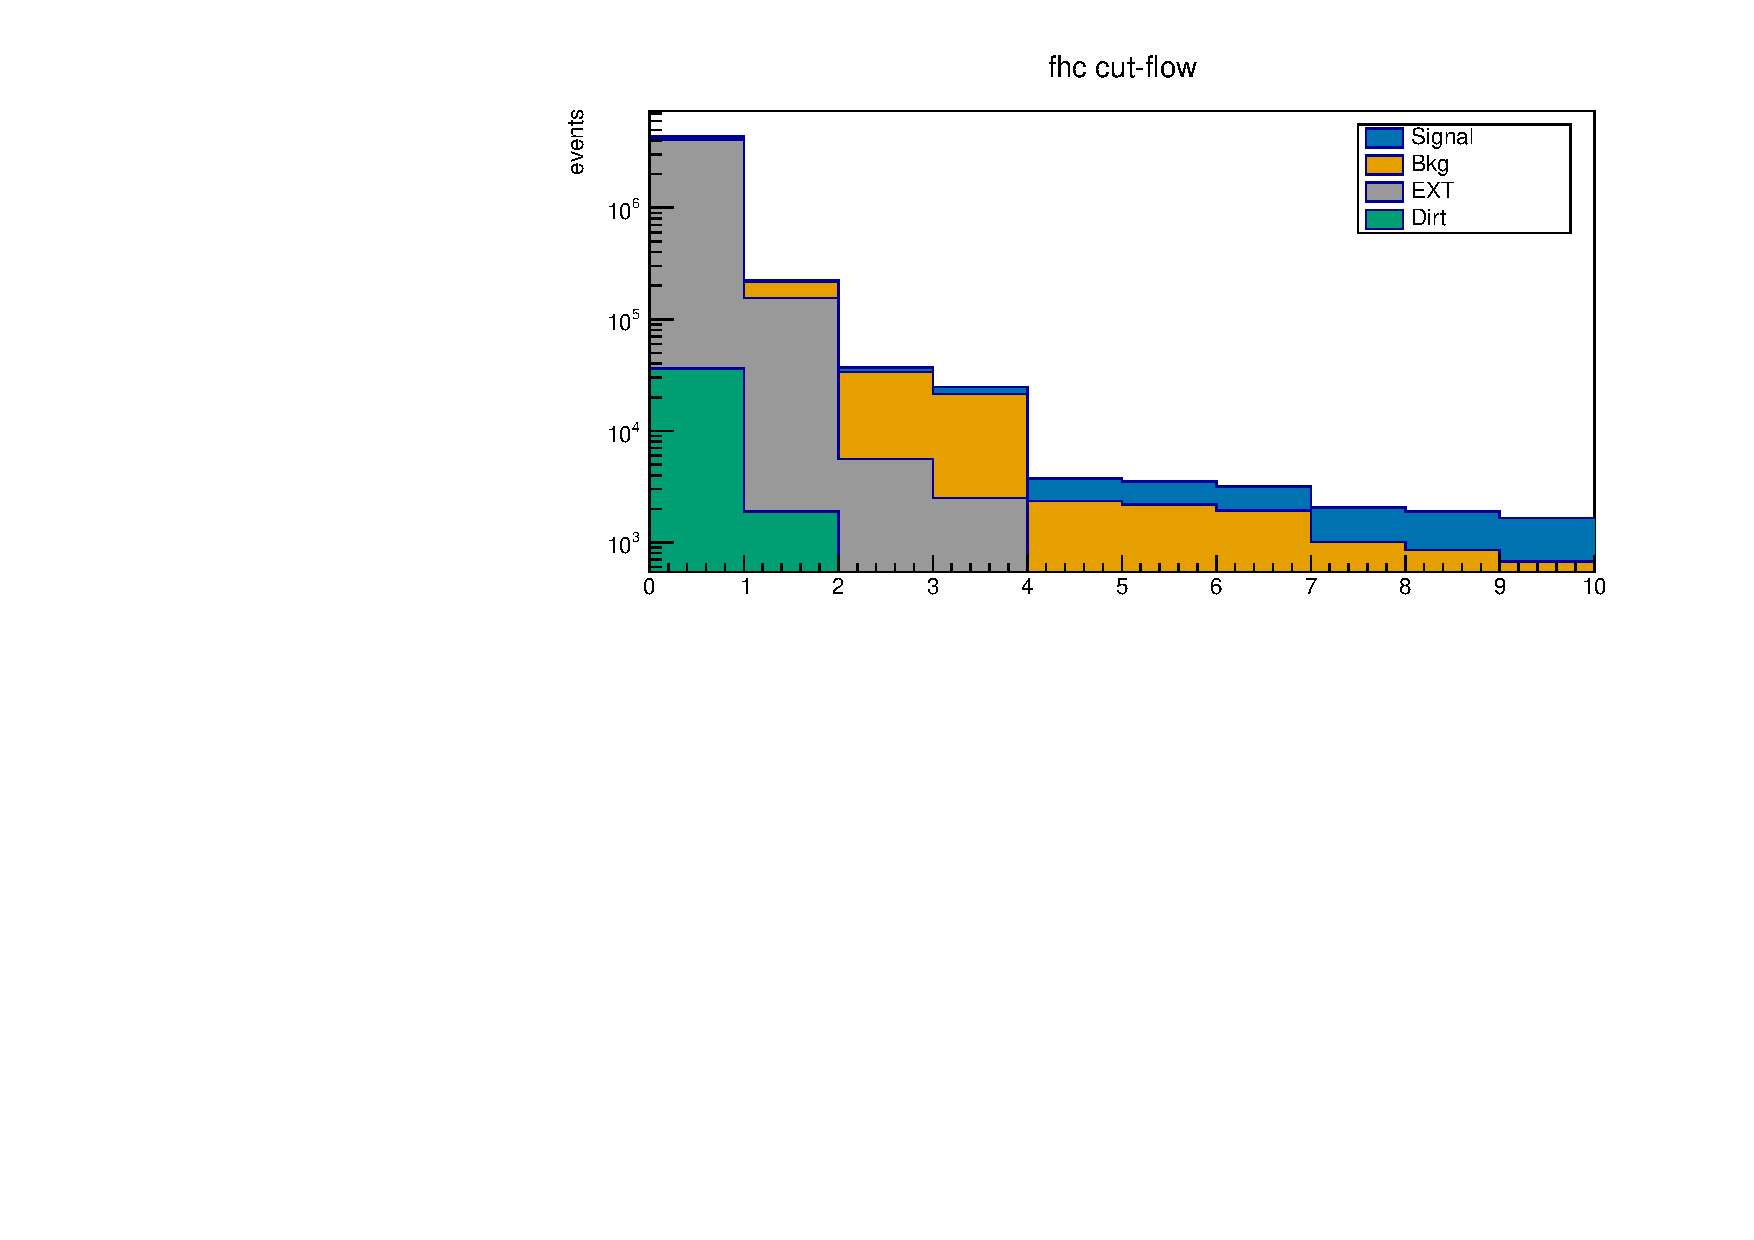
\includegraphics[width=\textwidth]{cutflow_yields_fhc}\caption{FHC.}\end{subfigure}\hfill
  \begin{subfigure}[b]{0.32\textwidth}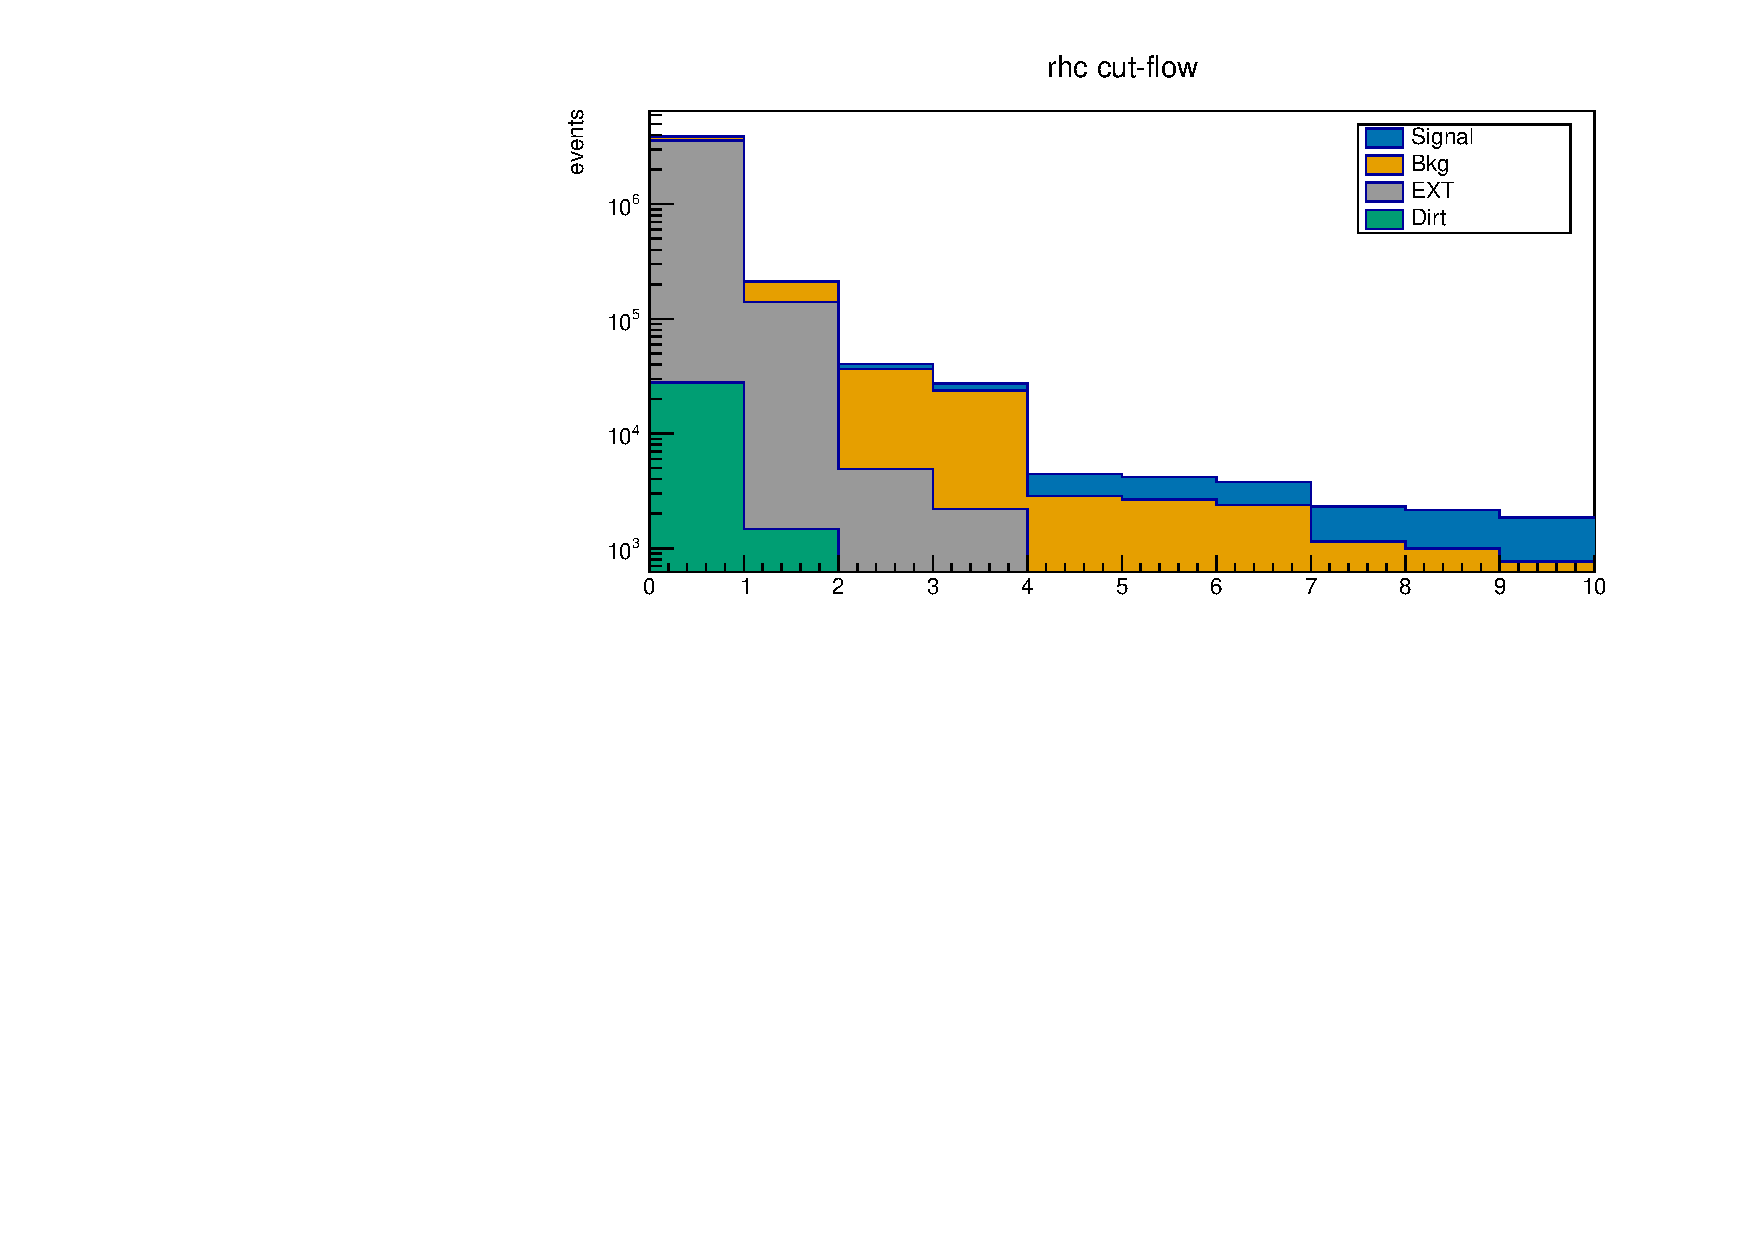
\includegraphics[width=\textwidth]{cutflow_yields_rhc}\caption{RHC.}\end{subfigure}\hfill
  \begin{subfigure}[b]{0.32\textwidth}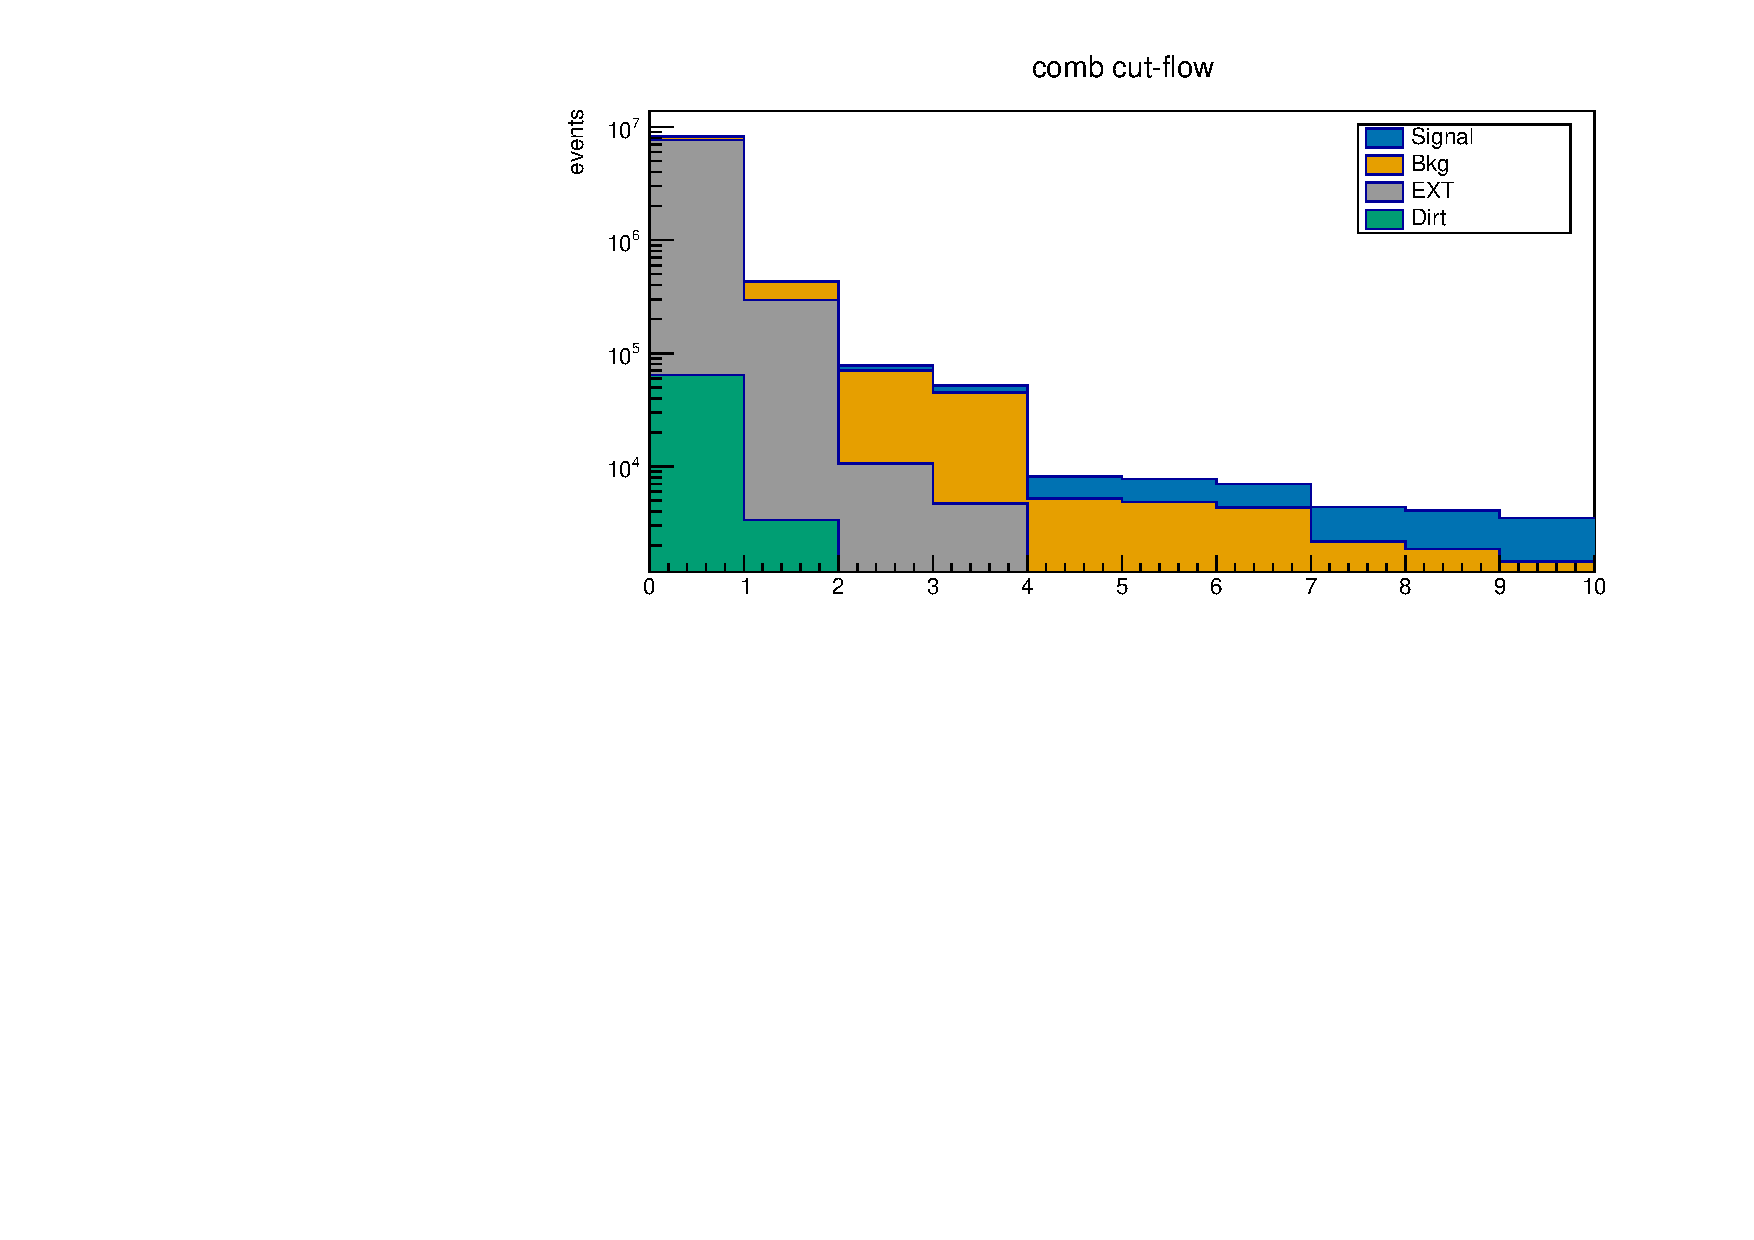
\includegraphics[width=\textwidth]{cutflow_yields_comb}\caption{Combined.}\end{subfigure}
  \caption{Cut-flow yields at \emph{full exposure} for FHC, RHC and combined
    (log scale; MC-prediction stack: signal blue, background orange, EXT grey,
    dirt green; colourblind-safe Okabe-Ito), signal and background POT-scaled per
    mode. Data is blind, so this shows the MC-prediction stack; the detailed
    per-category breakdown is in Table~\ref{tab:cutflow}.}
  \label{fig:cutflow_all}
\end{figure}

\begin{table}[H]
  \centering
  \caption{Cut-flow yields at \emph{full exposure} for FHC, RHC and combined
    (MC prediction; data is blind: the fake-data \emph{expectation} equals the
    central-value prediction by construction, while the realised pseudo-data fluctuate
    according to the Poisson throw). The histograms behind this table carry the
    framework's full central-value weight, tune $\times$ PPFX $\times$ normalisation
    (\S\ref{sec:mc}, with the safe-weight rule of Eq.~\eqref{eq:safeweight}), the same weight as the fake-data throw and
    the unfolding, so the final-cut yields agree with the cut-and-count
    Table~\ref{tab:cutcount} to $<1\%$. Signal and ``Bkg'' (all non-signal MC: OOFV, NC,
    CC1$\pi^0$, CC0$\pi$, CC$N\pi$, CCK, CCother) are from the $\nu_\mu$ overlays,
    POT-scaled \emph{per run} (each run by its own $D_{\text{run}}/\text{MC}_{\text{run}}$,
    Table~\ref{tab:pot}); EXT (beam-off cosmic) is scaled by the (per-run summed)
    per-run beam-on/beam-off \emph{gate} ratio times the $0.98$ NuMI beam-occupancy factor, each run period using the beam-off sample taken in that period (\S\ref{sec:mc}); dirt from the
    GENIE NuMI dirt overlay. Pred.\ $=$ Signal $+$ Bkg $+$ EXT $+$ Dirt. Eff.\ is the cumulative signal efficiency relative to the generated signal (the None stage, where all true signal is counted); Pur.\ $=$ Signal/Pred.}
  \label{tab:cutflow}
  \small
  \begin{tabular}{lrrrrrrr}
    \toprule
    Cut & Signal & Bkg MC & EXT & Dirt & Pred. & Eff. [\%] & Pur. [\%] \\
    \midrule
    \multicolumn{8}{l}{\textit{FHC (Runs 1,2,4,5; $8.857\times10^{20}$~POT)}} \\
    None & 5\,417 & 268\,316 & 4\,049\,292 & 33\,638 & 4\,356\,662 & 100.0 & 0.1 \\
    InFiducialVol & 4\,504 & 60\,235 & 153\,533 & 1\,763 & 220\,036 & 83.1 & 2.0 \\
    Topological & 3\,407 & 27\,640 & 5\,409 & 192 & 36\,647 & 62.9 & 9.3 \\
    MuonCandidate & 3\,056 & 18\,786 & 2\,363 & 129 & 24\,333 & 56.4 & 12.6 \\
    ContainedPion & 1\,358 & 2\,080 & 223 & 24 & 3\,685 & 25.1 & 36.8 \\
    MuonIn3Planes & 1\,299 & 1\,964 & 185 & 16 & 3\,464 & 24.0 & 37.5 \\
    PionIn3Planes & 1\,204 & 1\,759 & 144 & 6.8 & 3\,114 & 22.2 & 38.7 \\
    ShowerCut & 1\,016 & 891 & 108 & 5.8 & 2\,021 & 18.8 & 50.3 \\
    OpeningAngle & 1\,009 & 807 & 41 & 1.9 & 1\,859 & 18.6 & 54.3 \\
    \textbf{Nonprotons} & \textbf{943} & \textbf{637} & \textbf{30} & \textbf{1.3} & \textbf{1\,612} & \textbf{17.4} & \textbf{58.5} \\
    \midrule
    \multicolumn{8}{l}{\textit{RHC (Runs 1,2,3,4a,4b,4c; $1.108\times10^{21}$~POT)}} \\
    None & 5\,778 & 286\,540 & 3\,560\,975 & 26\,089 & 3\,879\,381 & 100.0 & 0.1 \\
    InFiducialVol & 4\,828 & 65\,474 & 139\,122 & 1\,367 & 210\,791 & 83.6 & 2.3 \\
    Topological & 3\,743 & 30\,446 & 4\,767 & 149 & 39\,104 & 64.8 & 9.6 \\
    MuonCandidate & 3\,363 & 20\,709 & 2\,090 & 100 & 26\,262 & 58.2 & 12.8 \\
    ContainedPion & 1\,488 & 2\,576 & 191 & 19 & 4\,274 & 25.7 & 34.8 \\
    MuonIn3Planes & 1\,426 & 2\,430 & 158 & 13 & 4\,028 & 24.7 & 35.4 \\
    PionIn3Planes & 1\,329 & 2\,194 & 121 & 5.3 & 3\,650 & 23.0 & 36.4 \\
    ShowerCut & 1\,101 & 1\,026 & 86 & 4.5 & 2\,218 & 19.1 & 49.7 \\
    OpeningAngle & 1\,093 & 933 & 33 & 1.5 & 2\,060 & 18.9 & 53.1 \\
    \textbf{Nonprotons} & \textbf{1\,015} & \textbf{720} & \textbf{23} & \textbf{1.0} & \textbf{1\,759} & \textbf{17.6} & \textbf{57.7} \\
    \midrule
    \multicolumn{8}{l}{\textit{Combined FHC$+$RHC ($1.994\times10^{21}$~POT)}} \\
    None & 11\,195 & 554\,856 & 7\,610\,266 & 59\,727 & 8\,236\,044 & 100.0 & 0.1 \\
    InFiducialVol & 9\,332 & 125\,709 & 292\,655 & 3\,130 & 430\,826 & 83.4 & 2.2 \\
    Topological & 7\,149 & 58\,086 & 10\,176 & 340 & 75\,752 & 63.9 & 9.4 \\
    MuonCandidate & 6\,419 & 39\,495 & 4\,453 & 228 & 50\,595 & 57.3 & 12.7 \\
    ContainedPion & 2\,845 & 4\,656 & 414 & 43 & 7\,958 & 25.4 & 35.8 \\
    MuonIn3Planes & 2\,725 & 4\,394 & 343 & 29 & 7\,492 & 24.3 & 36.4 \\
    PionIn3Planes & 2\,533 & 3\,954 & 266 & 12 & 6\,764 & 22.6 & 37.4 \\
    ShowerCut & 2\,117 & 1\,917 & 194 & 10 & 4\,238 & 18.9 & 50.0 \\
    OpeningAngle & 2\,102 & 1\,740 & 74 & 3.3 & 3\,919 & 18.8 & 53.6 \\
    \textbf{Nonprotons} & \textbf{1\,959} & \textbf{1\,357} & \textbf{53} & \textbf{2.3} & \textbf{3\,372} & \textbf{17.5} & \textbf{58.1} \\
    \bottomrule
  \end{tabular}
\end{table}

\paragraph{Why the phase space and the opening-angle cut are what they are.}
The thresholds were chosen from the efficiency turn-ons and purity studies on the Run-1
FHC sample (\suppref{Sec.}{sec:supp_optim}); the measured phase space removes the
near-zero-efficiency momentum regions and the low-purity large-opening-angle region. On
the full exposure the events the $\theta_{\mu\pi}<2.6$~rad cut removes are exactly those
of the cosmic control region (Table~\ref{tab:sideband_yields}): in FHC $6.0$ signal, $69$
neutrino background, $53$ beam-off and $2.2$ dirt, a signal purity of $4.6\%$. Dropping
the cut would lower the signal-region purity from $58.5\%$ to $54.5\%$, raise its
beam-off content from $30$ to $83$ events and recover only $2.7\%$ of the generated
signal. No lower opening-angle cut is used because the small-angle region is high-purity
($\sim\!58\%$), so cutting it lowers the selected signal without improving purity. The
per-run exposure scaling of the yields differs from a single per-mode factor by about
$2\%$ in the final-cut signal, a nearly uniform re-weighting that moves efficiency and
purity by $<0.5\%$.

\subsection{Key N$-$1 distributions}

Figure~\ref{fig:nm1_key} shows the N$-$1 distributions (all cuts applied except
the one under study) for the two cuts instrumented per event; the topological
score (Cut~3) and the $\mu$--$\pi$ opening angle (Cut~9), for all three
configurations. The shapes are consistent across horn modes, as expected since
the selection is identical; RHC and combined simply carry the larger exposure.
Signal (blue) and background (orange) are stacked and the dashed line marks the
applied threshold. The remaining cut variables are shown at the final cut in
Sec.~\ref{sec:finalcut}.

\begin{figure}[H]
  \centering
  \begin{subfigure}[b]{0.32\textwidth}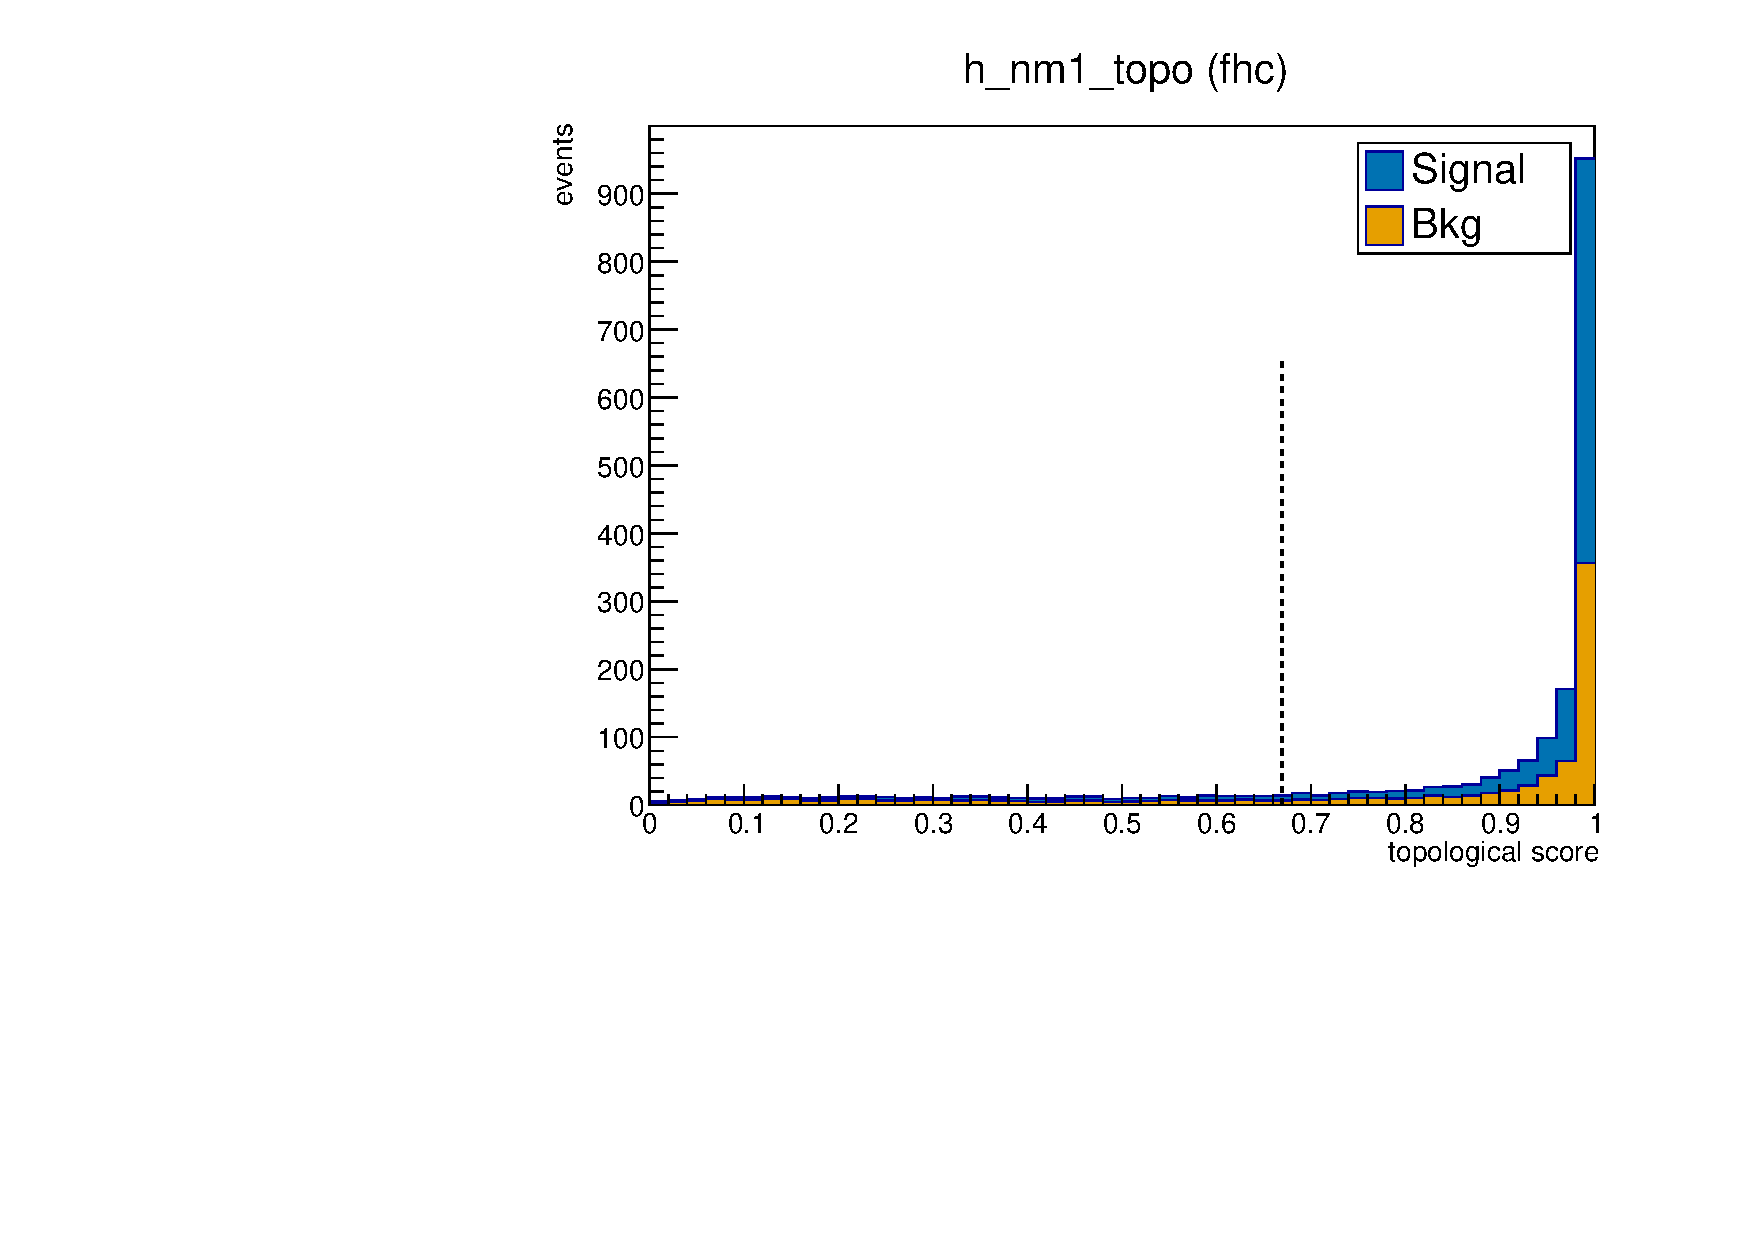
\includegraphics[width=\textwidth]{nm1_topo_fhc}\caption{Topo.\ score, FHC.}\end{subfigure}\hfill
  \begin{subfigure}[b]{0.32\textwidth}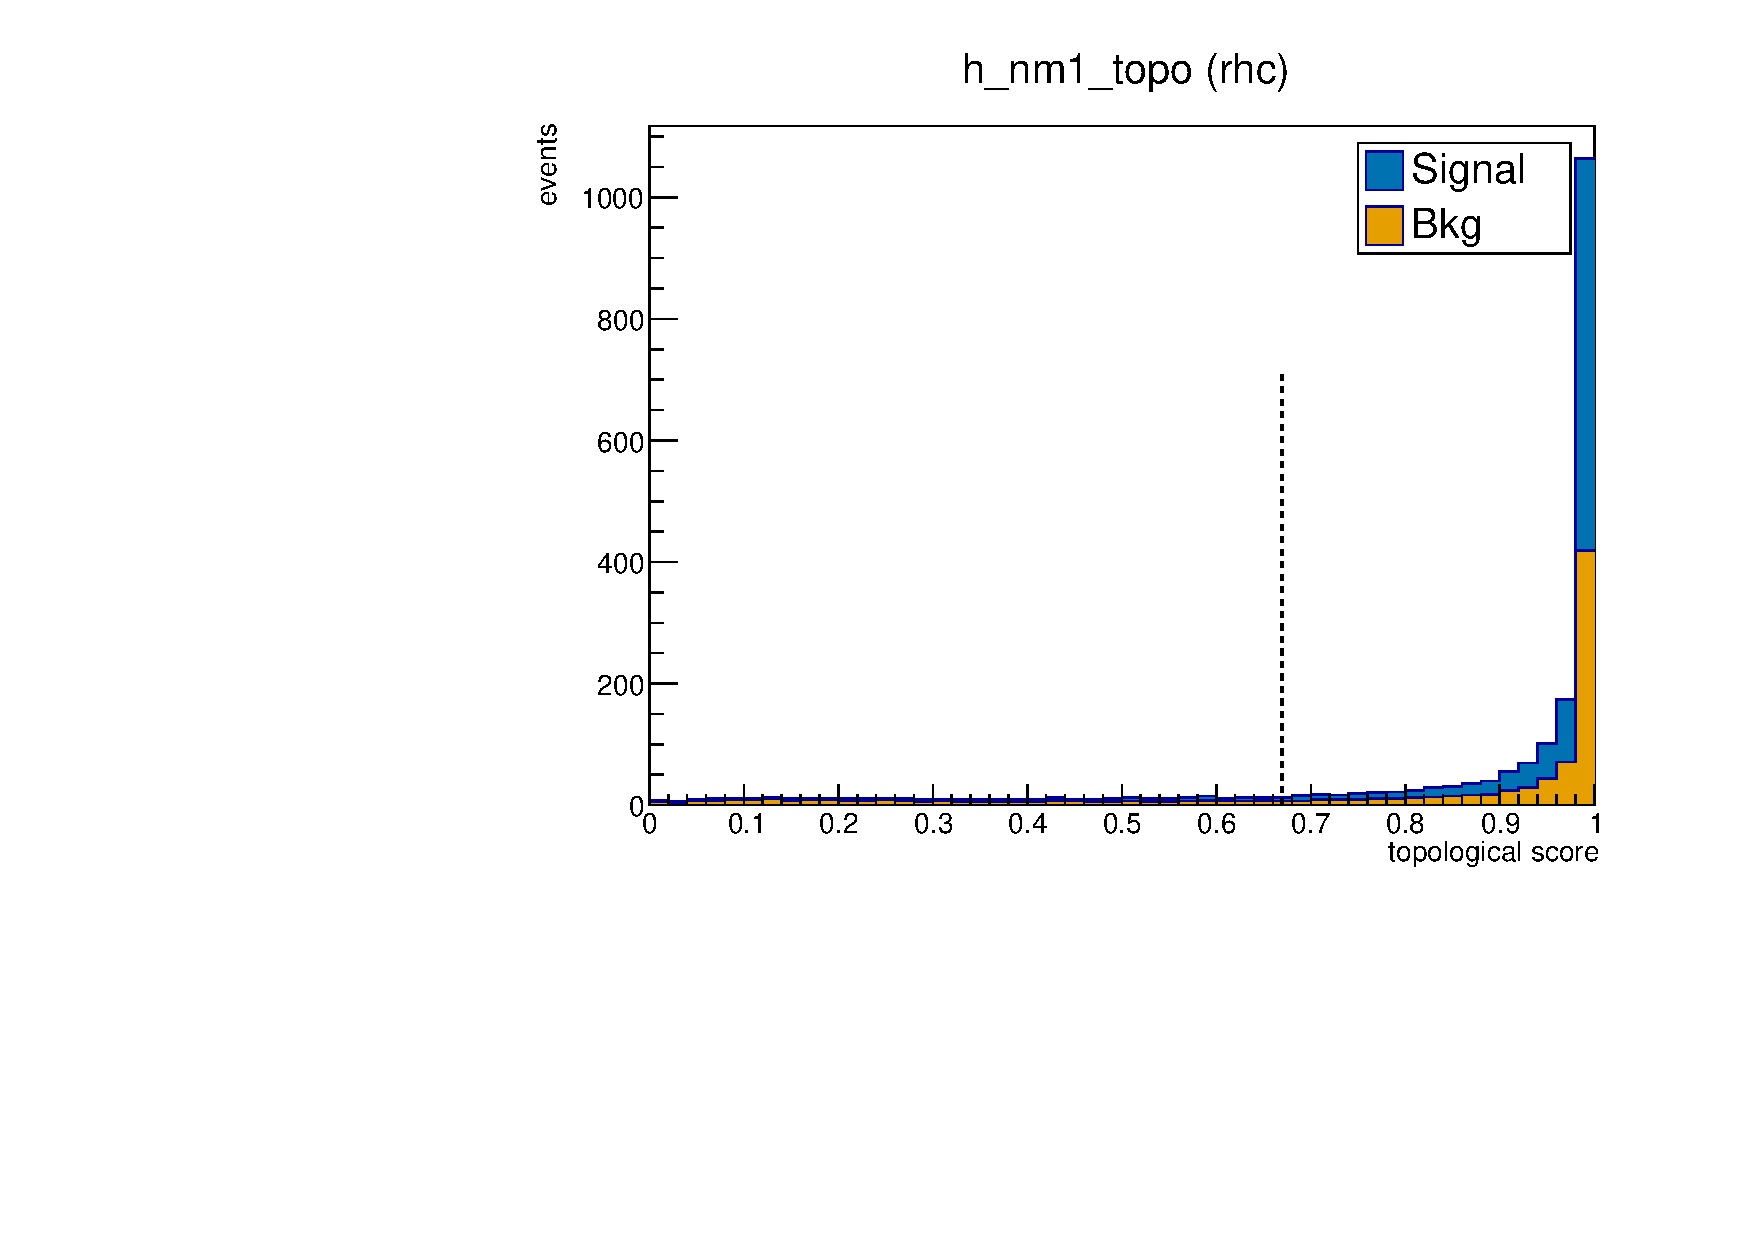
\includegraphics[width=\textwidth]{nm1_topo_rhc}\caption{Topo.\ score, RHC.}\end{subfigure}\hfill
  \begin{subfigure}[b]{0.32\textwidth}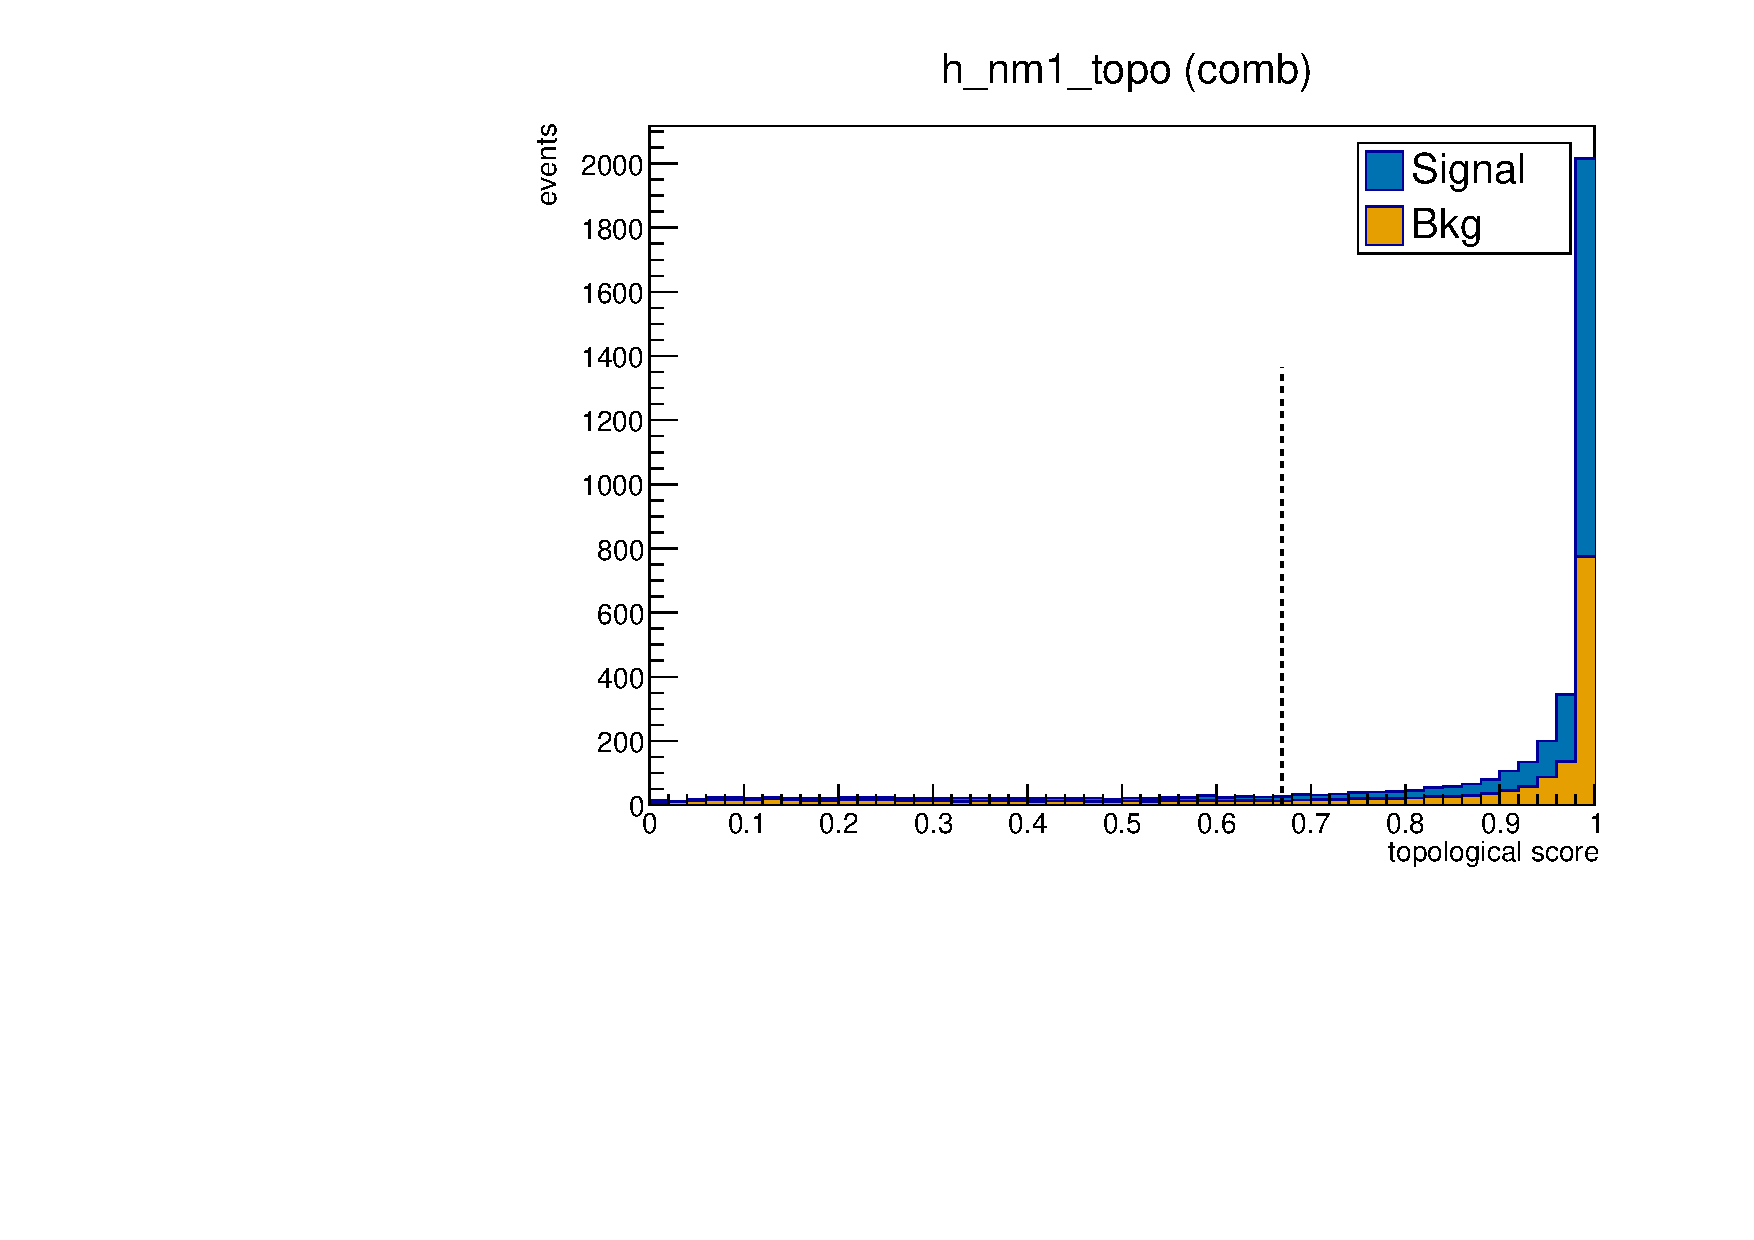
\includegraphics[width=\textwidth]{nm1_topo_comb}\caption{Topo.\ score, comb.}\end{subfigure}\\[6pt]
  \begin{subfigure}[b]{0.32\textwidth}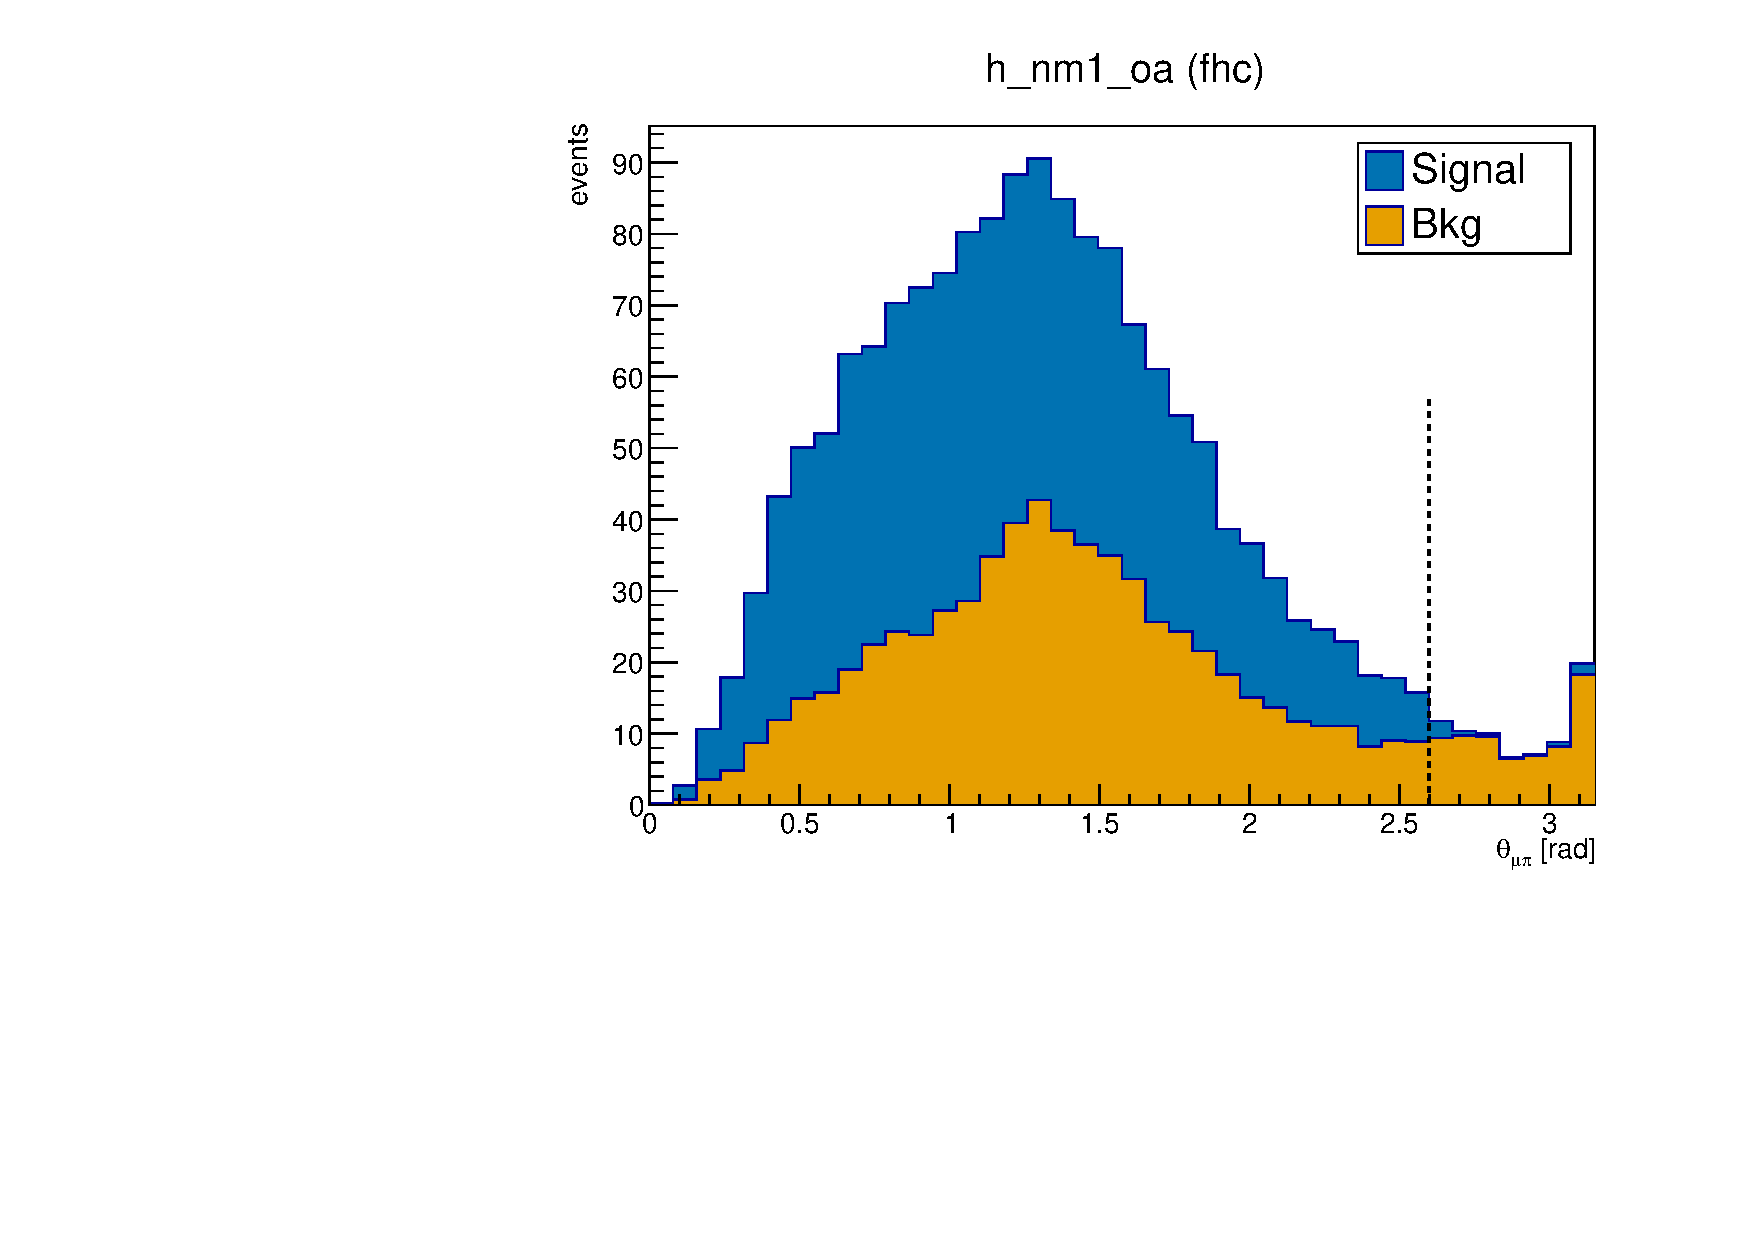
\includegraphics[width=\textwidth]{nm1_oa_fhc}\caption{Opening angle, FHC.}\end{subfigure}\hfill
  \begin{subfigure}[b]{0.32\textwidth}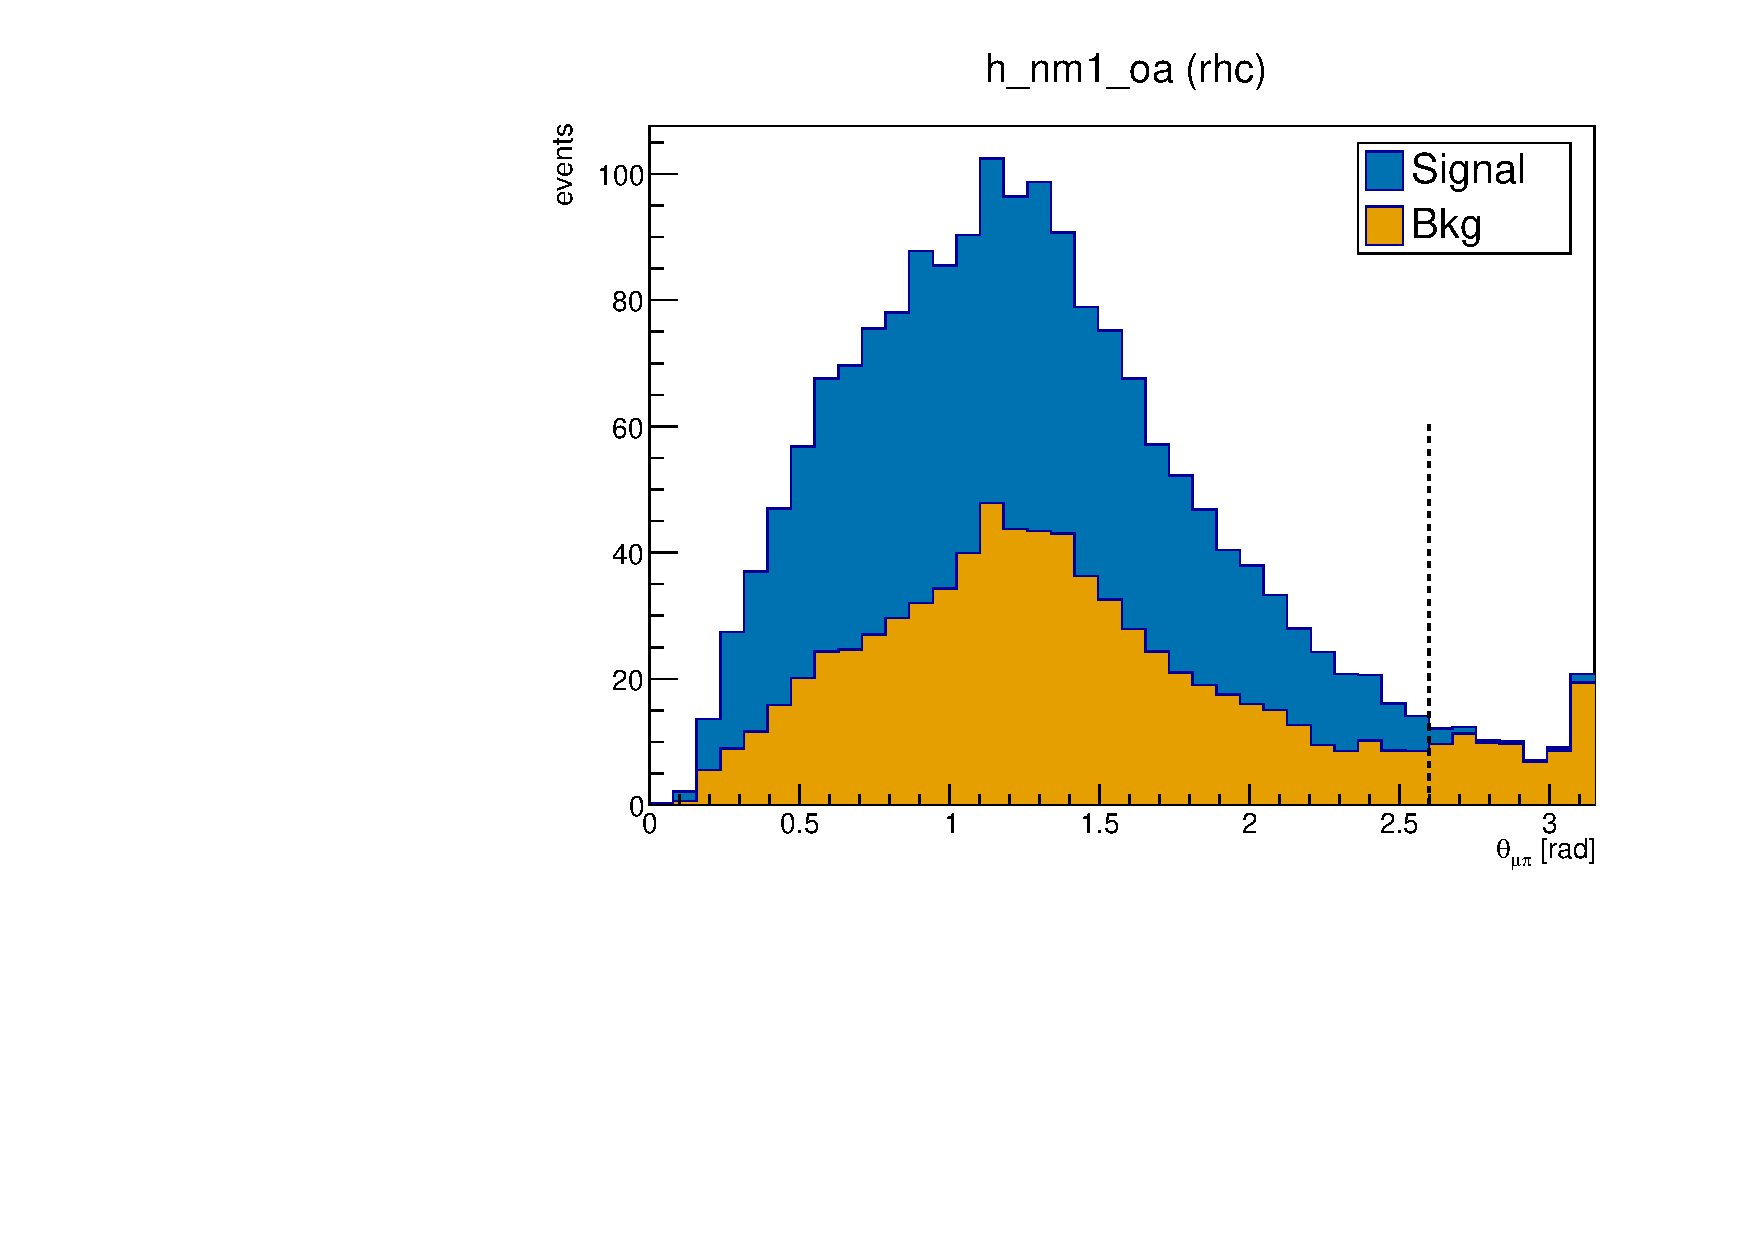
\includegraphics[width=\textwidth]{nm1_oa_rhc}\caption{Opening angle, RHC.}\end{subfigure}\hfill
  \begin{subfigure}[b]{0.32\textwidth}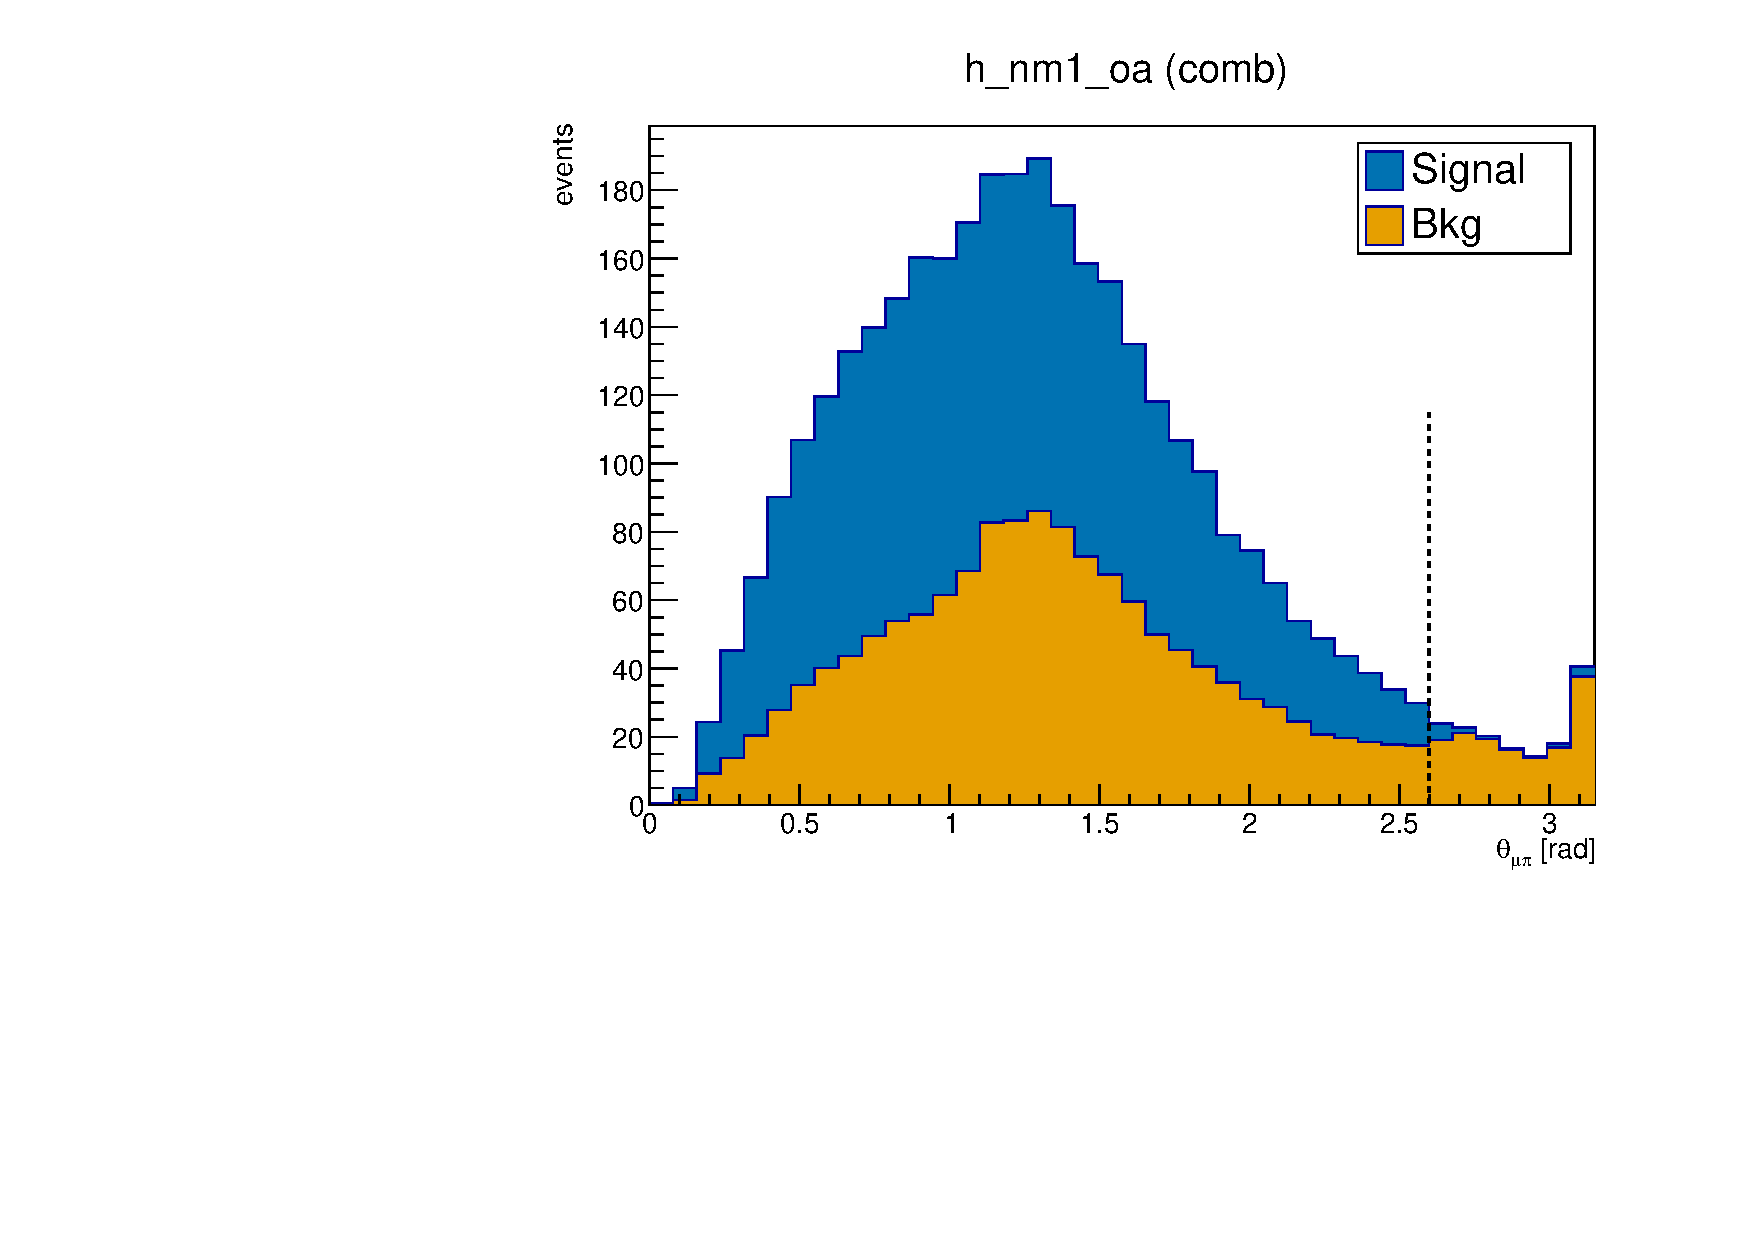
\includegraphics[width=\textwidth]{nm1_oa_comb}\caption{Opening angle, comb.}\end{subfigure}
  \caption{N$-$1 distributions for the topological score (Cut~3, top) and
    $\mu$--$\pi$ opening angle (Cut~9, bottom), for FHC, RHC and combined.
    Signal (blue) and background (orange) stacked; dashed line = applied
    threshold. Colourblind-safe Okabe-Ito palette.}
  \label{fig:nm1_key}
\end{figure}

\subsection{Pion proton-rejection variables}

Figure~\ref{fig:pid_proton} shows the two main proton-rejection variables on
the pion candidate, evaluated on MC truth-labelled pions ($\pi^\pm$) and
protons at the final cut stage, used to tune the working-point thresholds.

\begin{figure}[H]
  \centering
  \begin{subfigure}[b]{0.48\textwidth}
    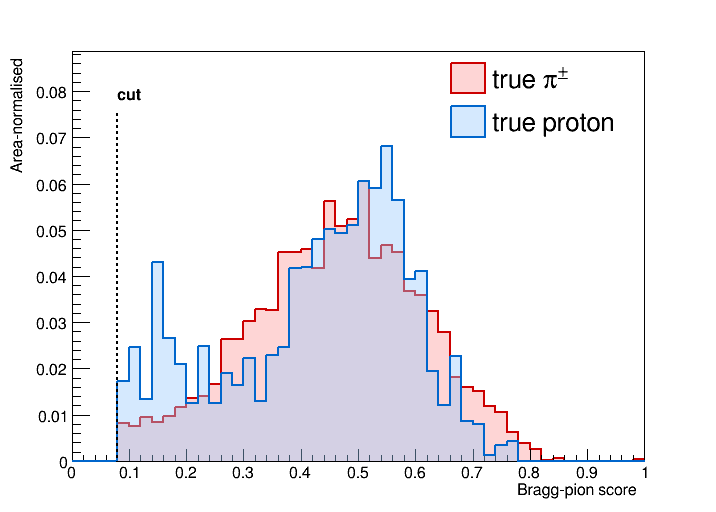
\includegraphics[width=\textwidth]{pid_bpion}
    \caption{Bragg-pion score.
      Working-point threshold: $\geq 0.08$.}
  \end{subfigure}
  \hfill
  \begin{subfigure}[b]{0.48\textwidth}
    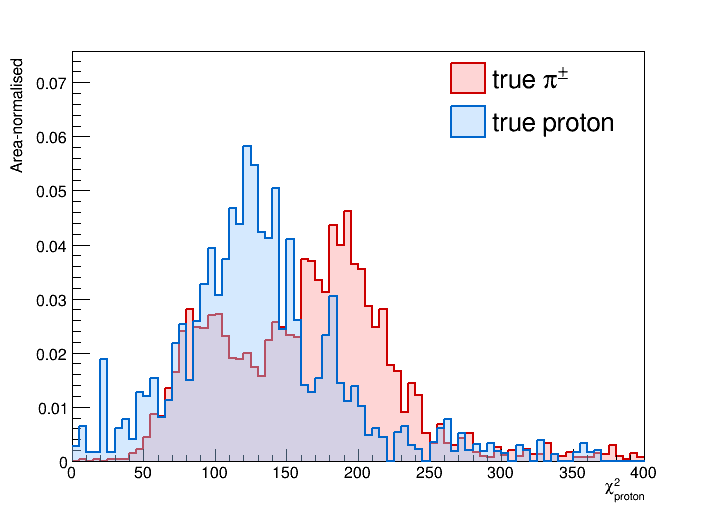
\includegraphics[width=\textwidth]{pid_chipr}
    \caption{$\chi^2$ proton PID.}
  \end{subfigure}
  \caption{Pion-candidate PID distributions for true $\pi^\pm$ (red) and
    true protons (blue) at the final cut stage.  The Bragg-pion score
    provides the primary proton rejection; $\chi^2_p$ is studied as
    cross-check.}
  \label{fig:pid_proton}
\end{figure}

\subsection{Final-cut data/MC distributions}
\label{sec:finalcut}

Figures~\ref{fig:final_mu} and~\ref{fig:final_pi} show the candidate-level
distributions at the final selection cut for the four instrumented PID and
track-length variables, for FHC and RHC. Signal (blue) and
background (orange) are stacked (colourblind-safe Okabe-Ito palette).

\begin{figure}[H]
  \centering
  \begin{subfigure}[b]{0.32\textwidth}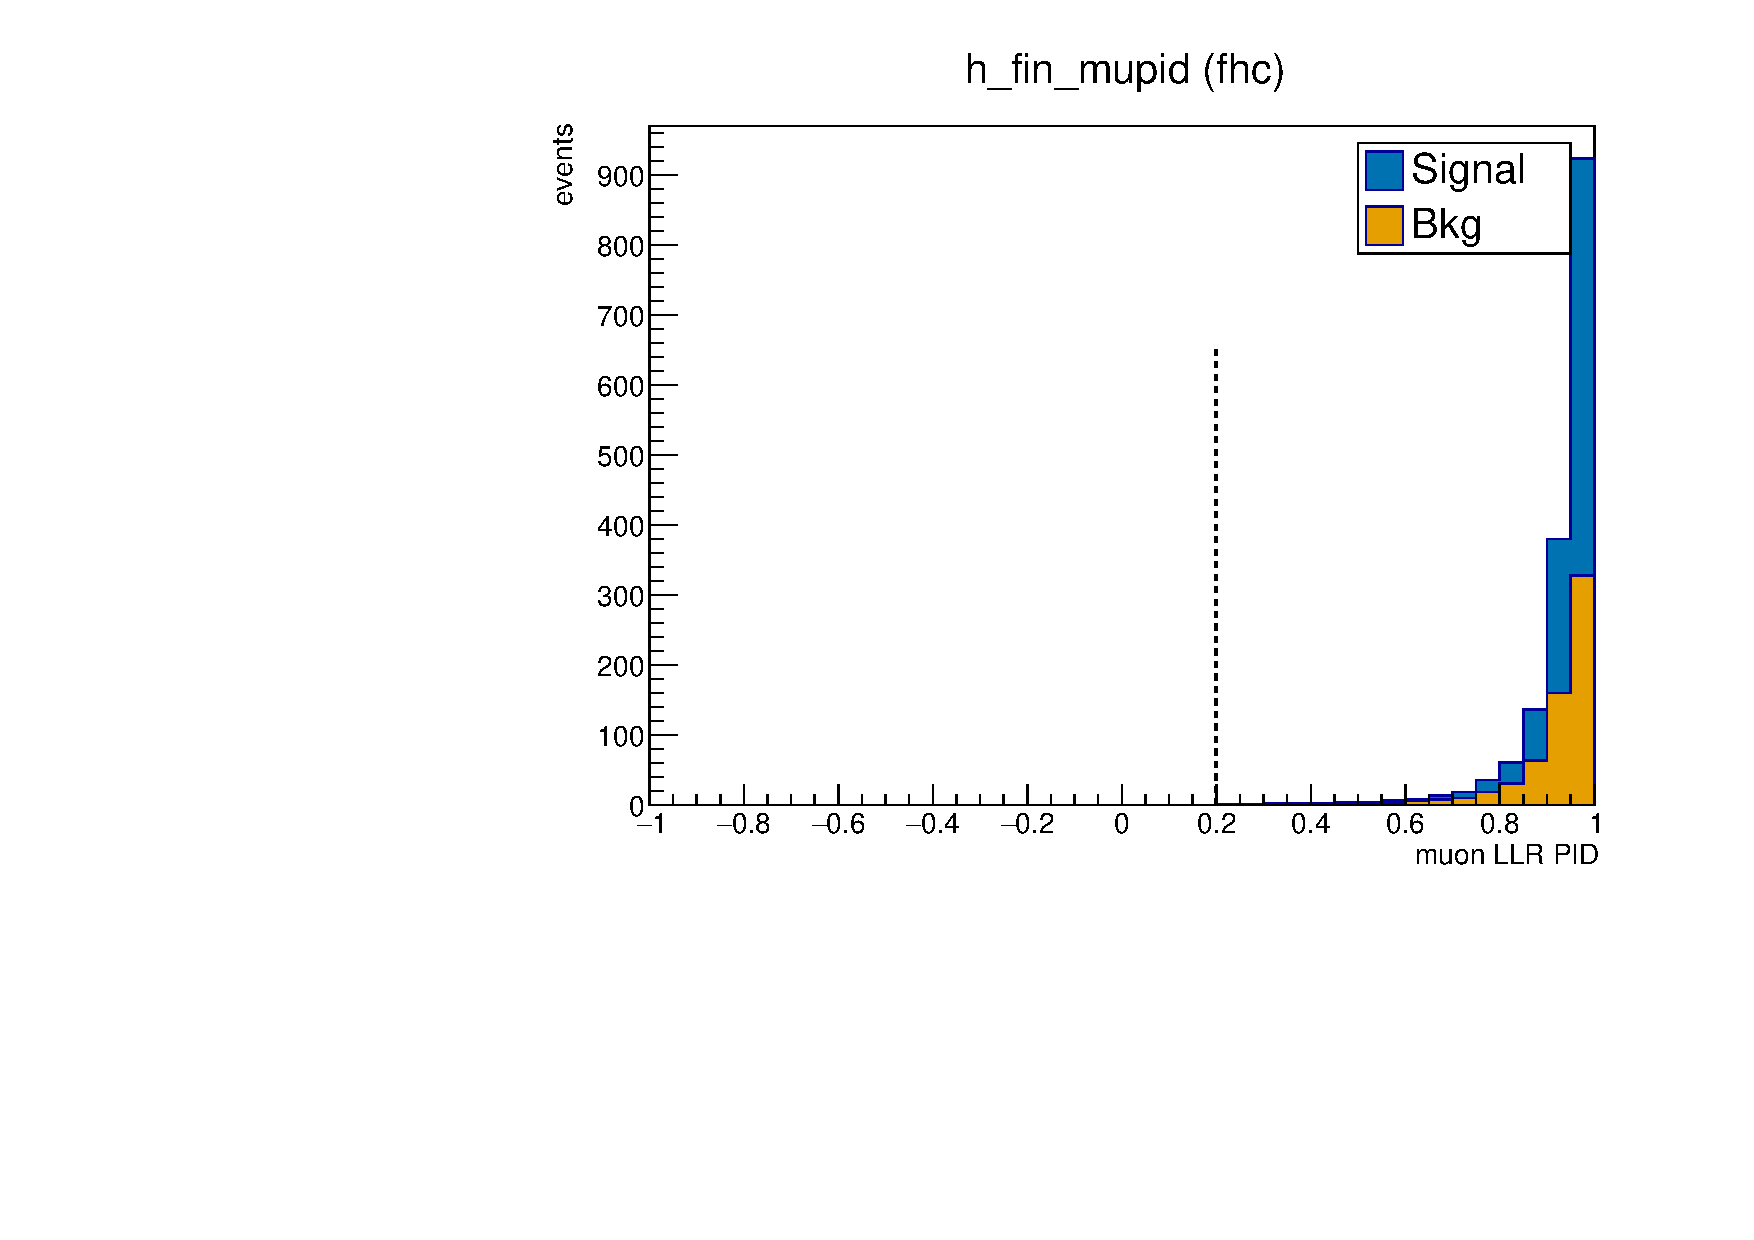
\includegraphics[width=\textwidth]{final_mupid_fhc}\caption{Muon LLR PID, FHC.}\end{subfigure}\hfill
  \begin{subfigure}[b]{0.32\textwidth}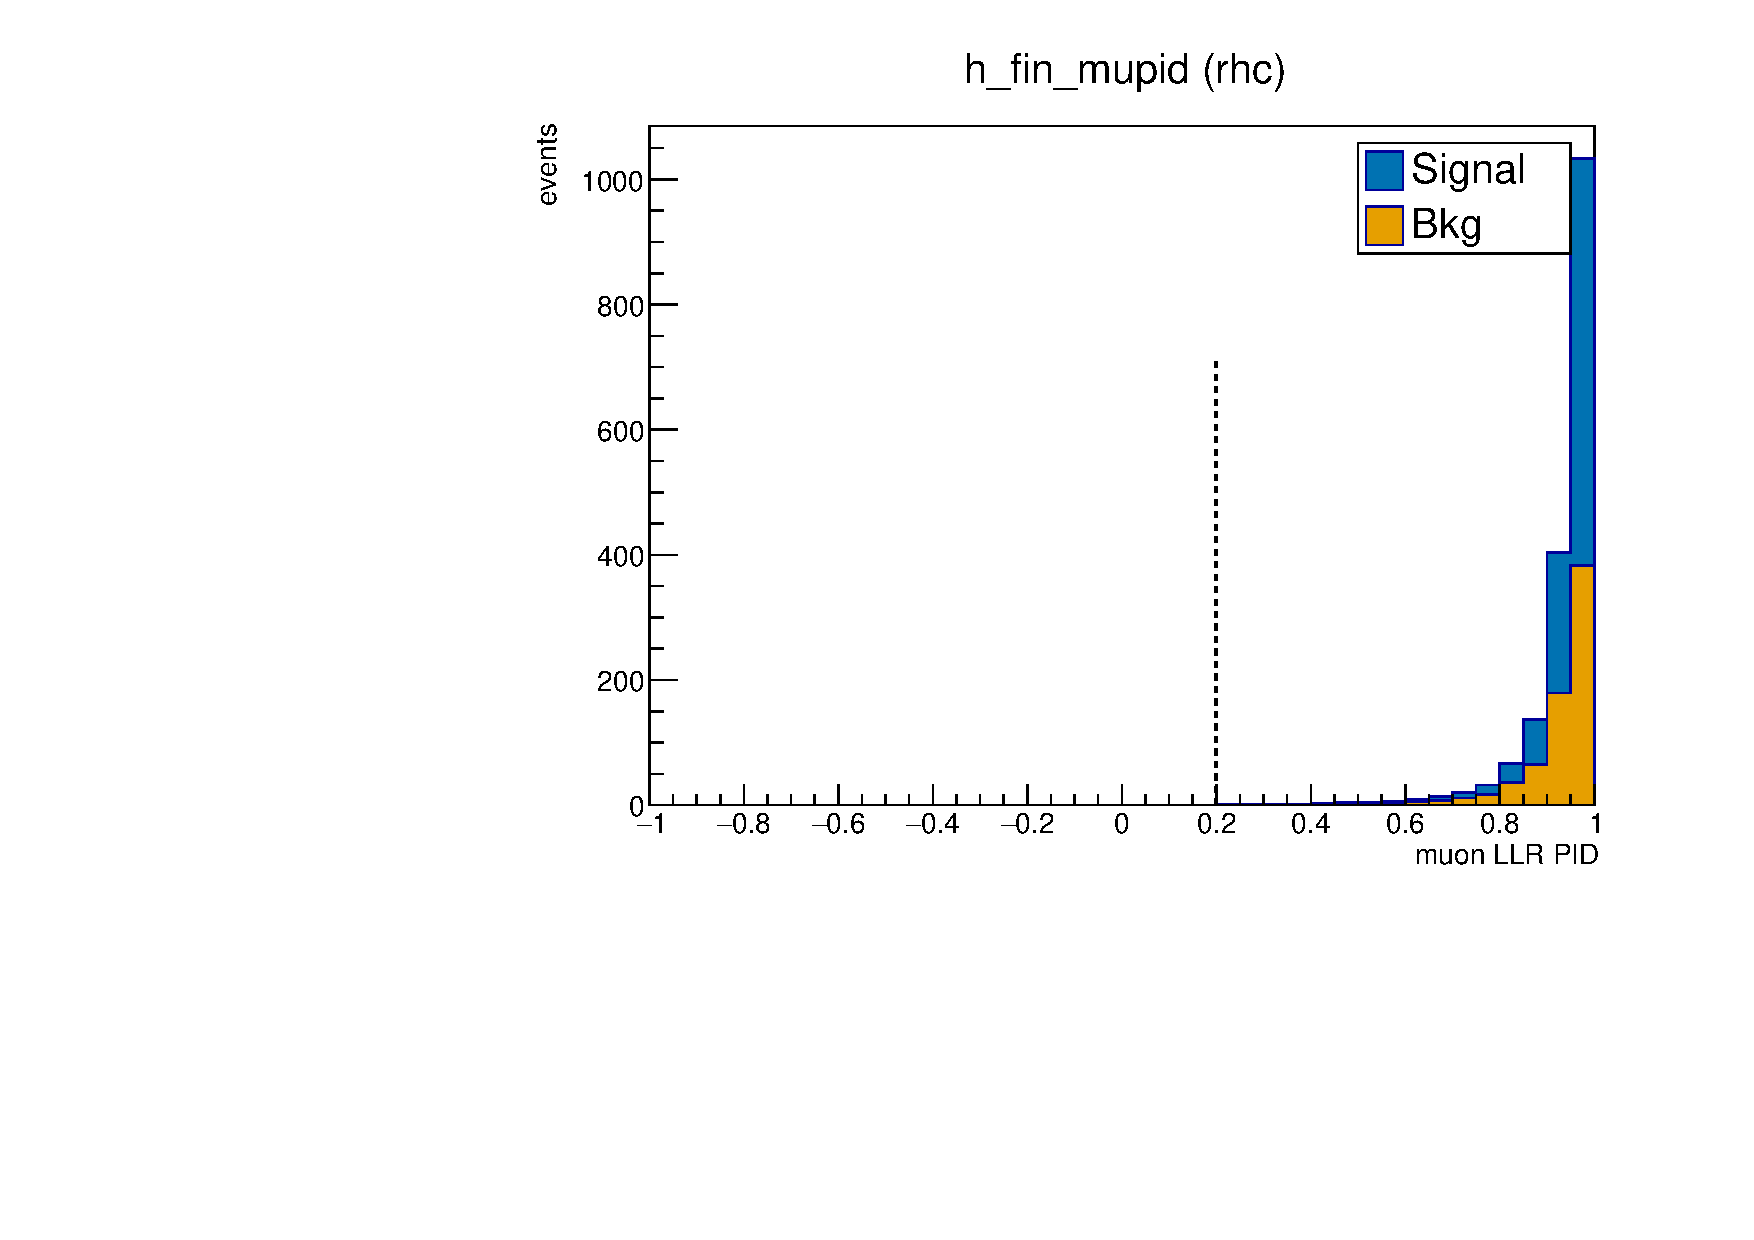
\includegraphics[width=\textwidth]{final_mupid_rhc}\caption{Muon LLR PID, RHC.}\end{subfigure}\hfill\\[6pt]
  \begin{subfigure}[b]{0.32\textwidth}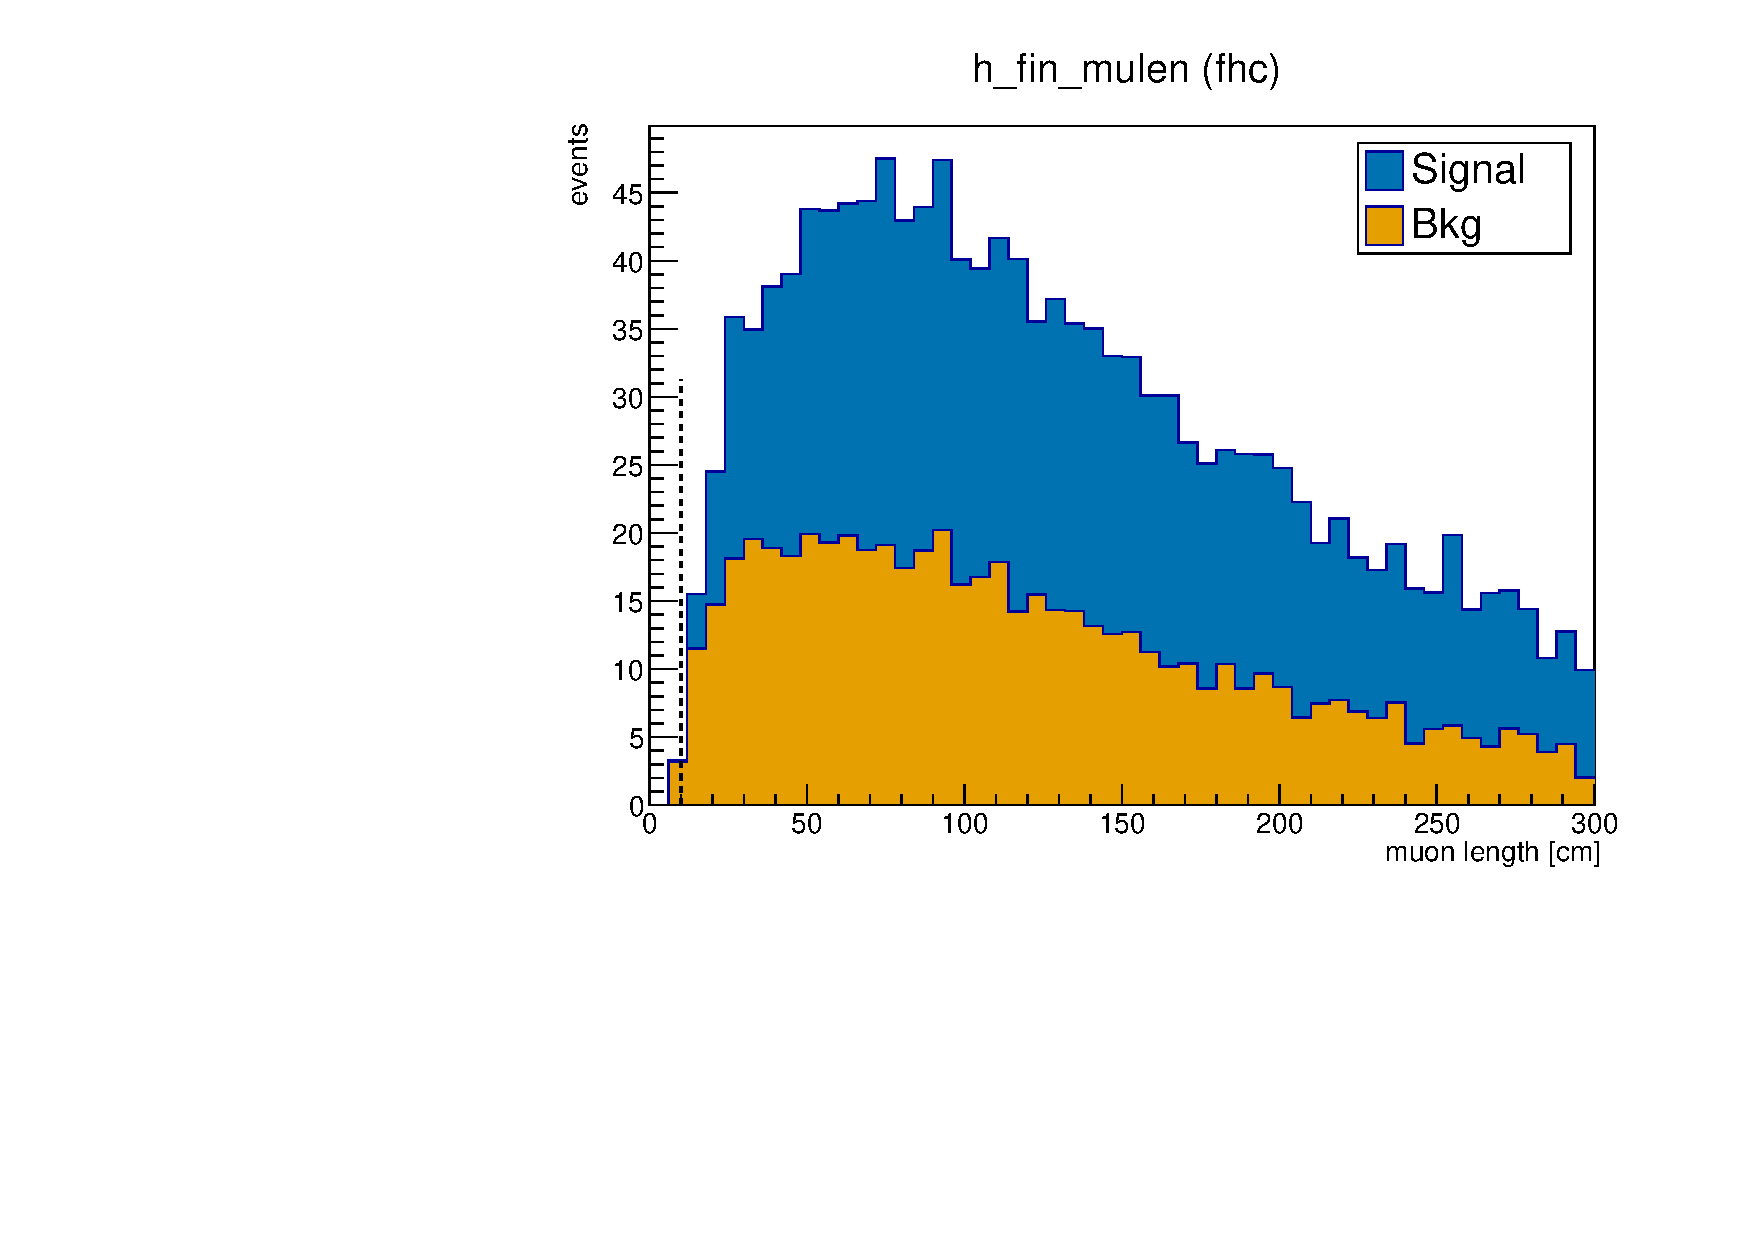
\includegraphics[width=\textwidth]{final_mulen_fhc}\caption{Muon length, FHC.}\end{subfigure}\hfill
  \begin{subfigure}[b]{0.32\textwidth}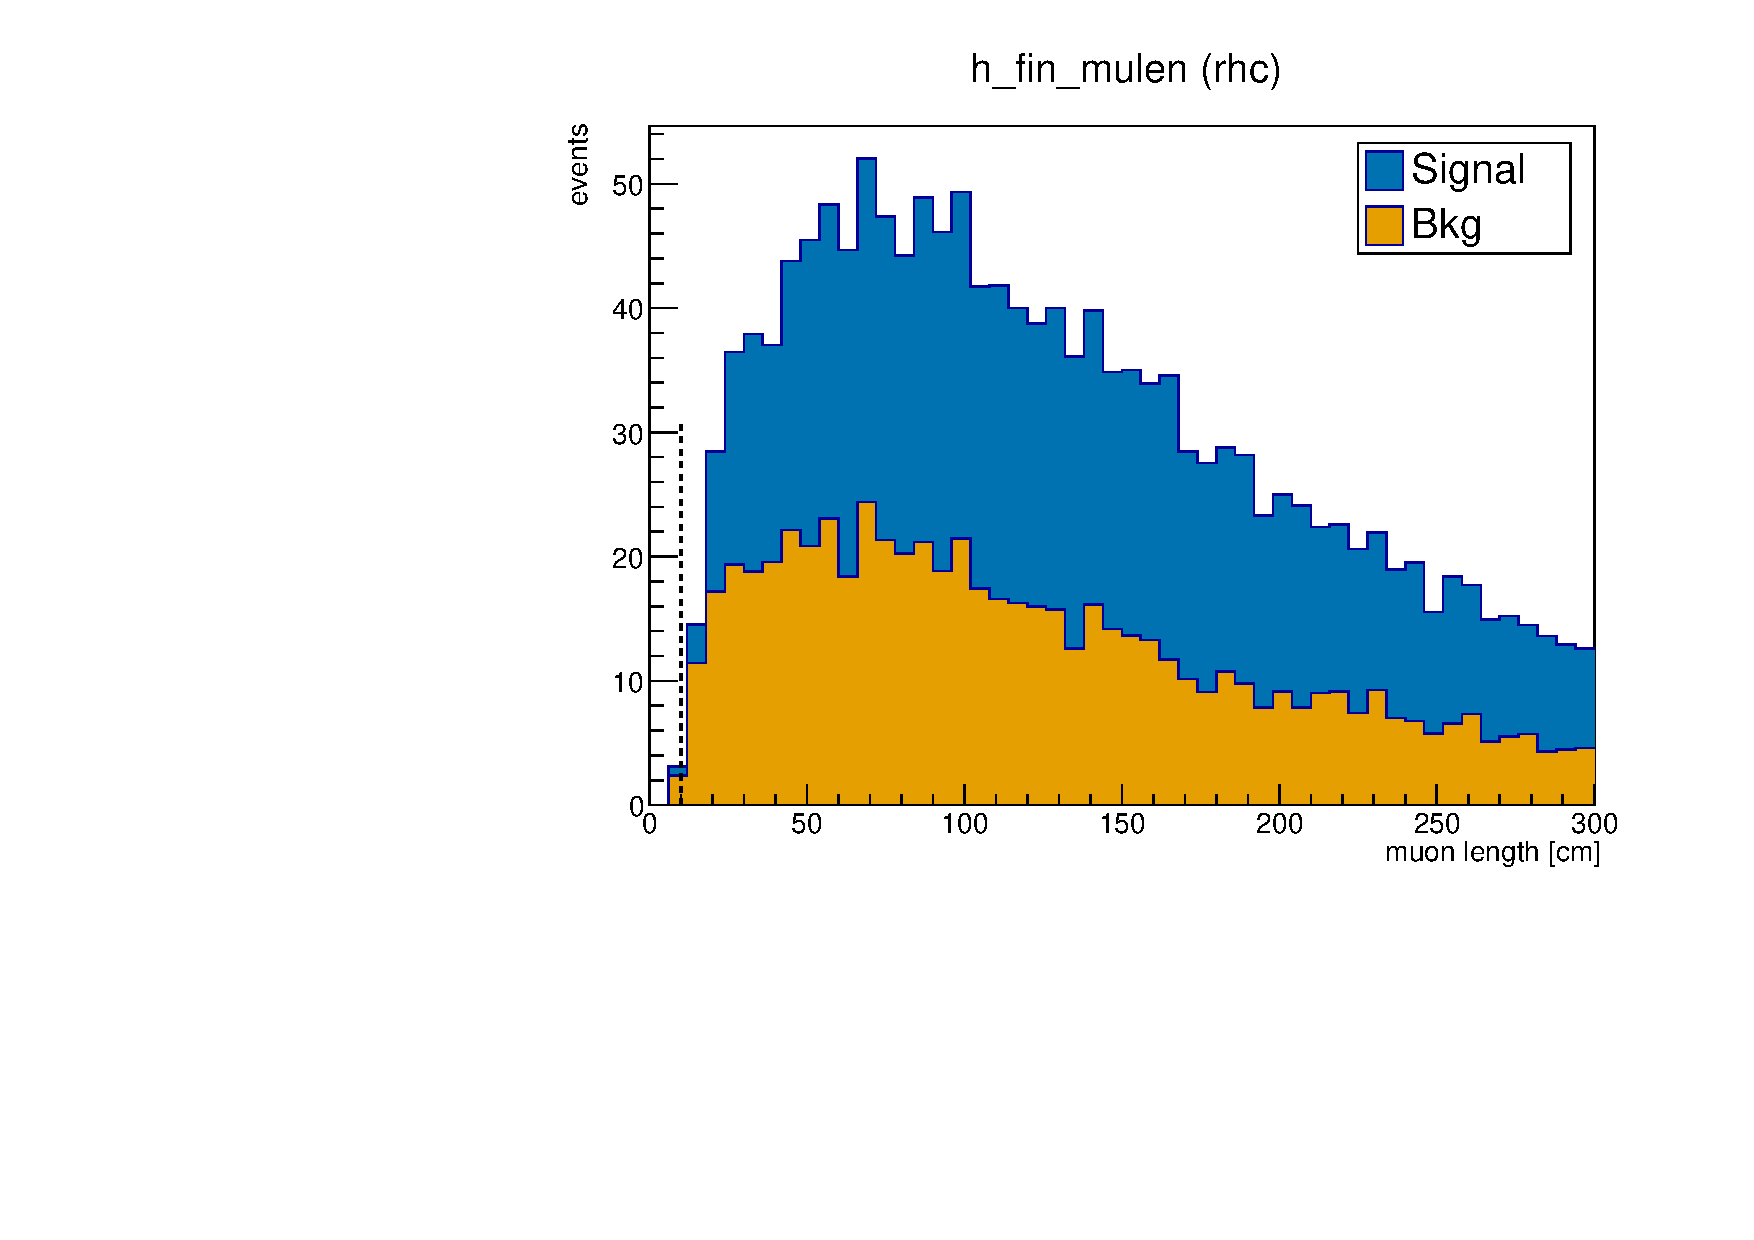
\includegraphics[width=\textwidth]{final_mulen_rhc}\caption{Muon length, RHC.}\end{subfigure}\hfill
  \caption{Muon-candidate LLR PID (top) and track length (bottom) at the final
    cut, for FHC and RHC (the combined configuration is consistent with both and is not
    shown). Signal (blue) / background (orange) stacked.}
  \label{fig:final_mu}
\end{figure}

\begin{figure}[H]
  \centering
  \begin{subfigure}[b]{0.32\textwidth}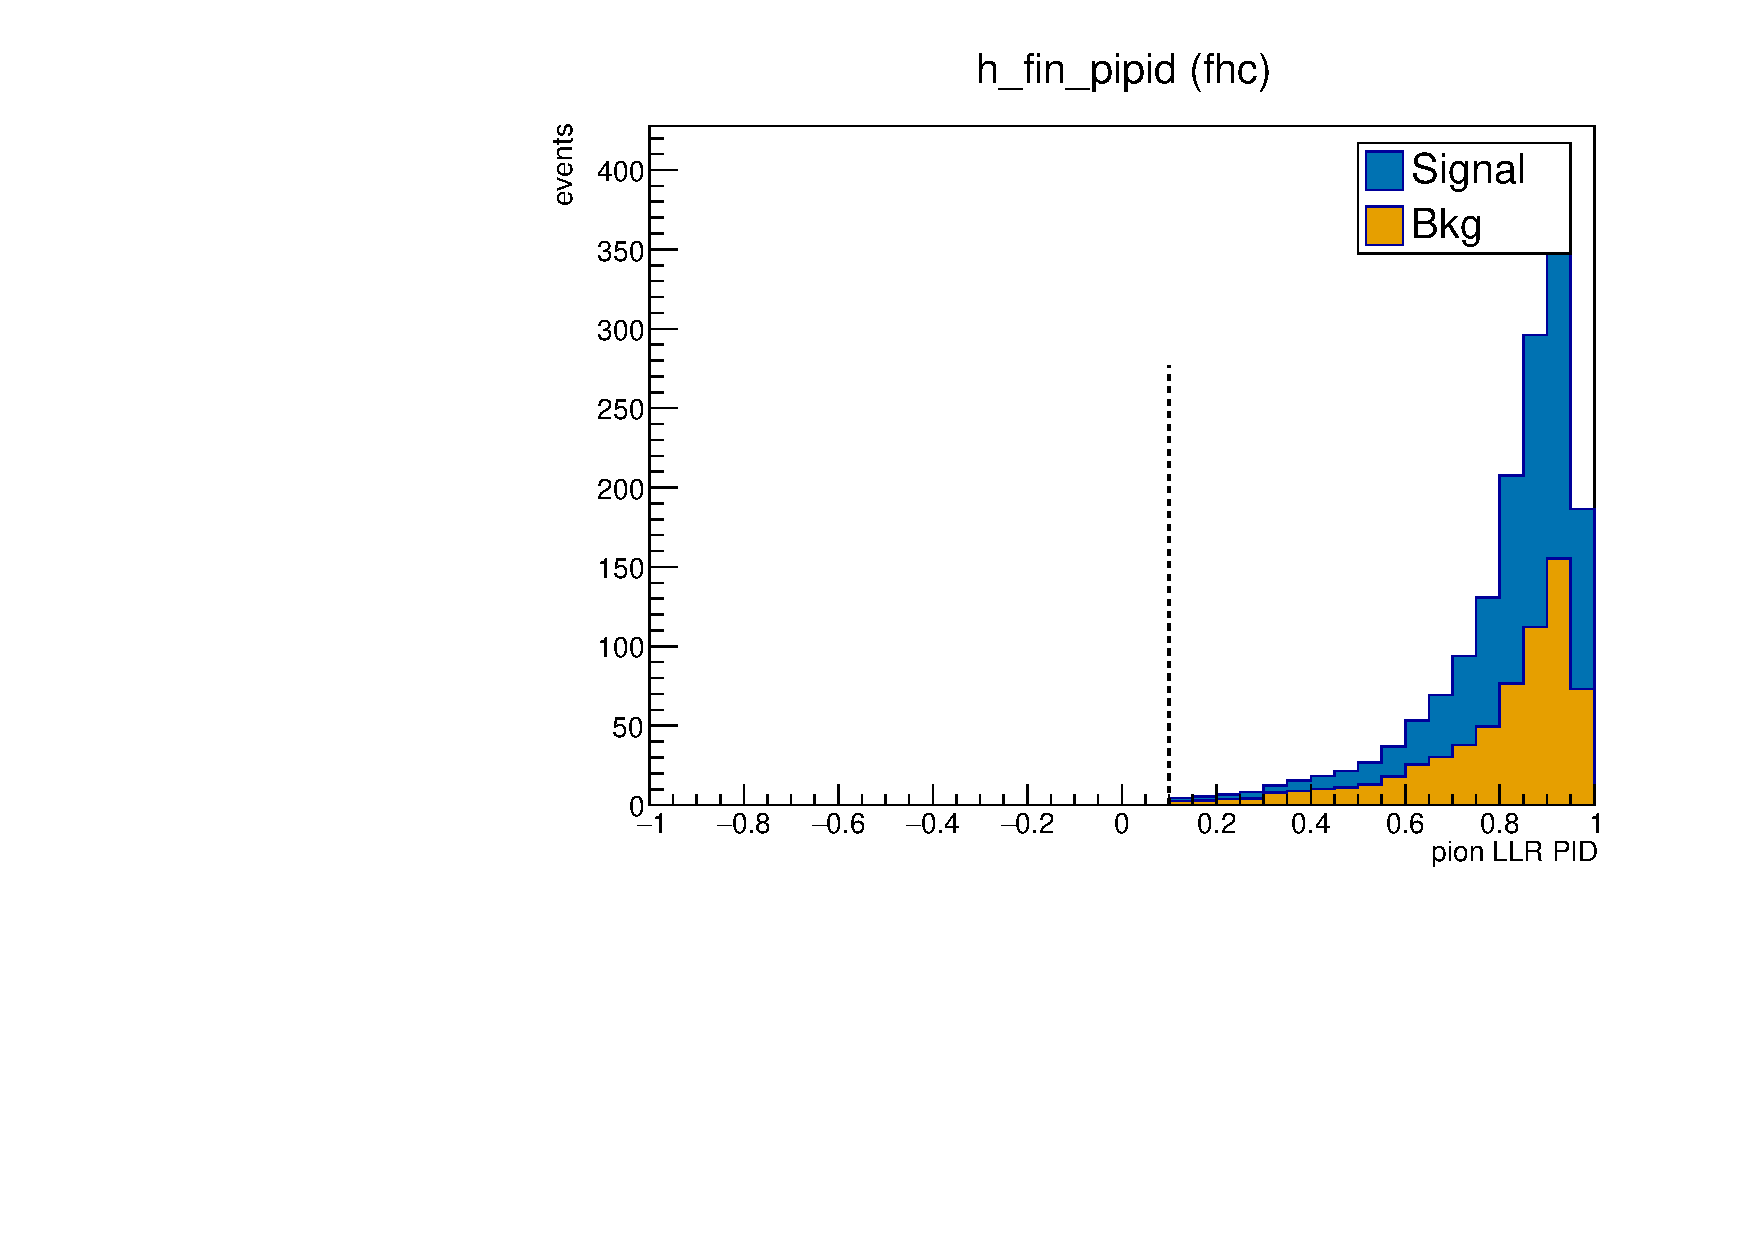
\includegraphics[width=\textwidth]{final_pipid_fhc}\caption{Pion LLR PID, FHC.}\end{subfigure}\hfill
  \begin{subfigure}[b]{0.32\textwidth}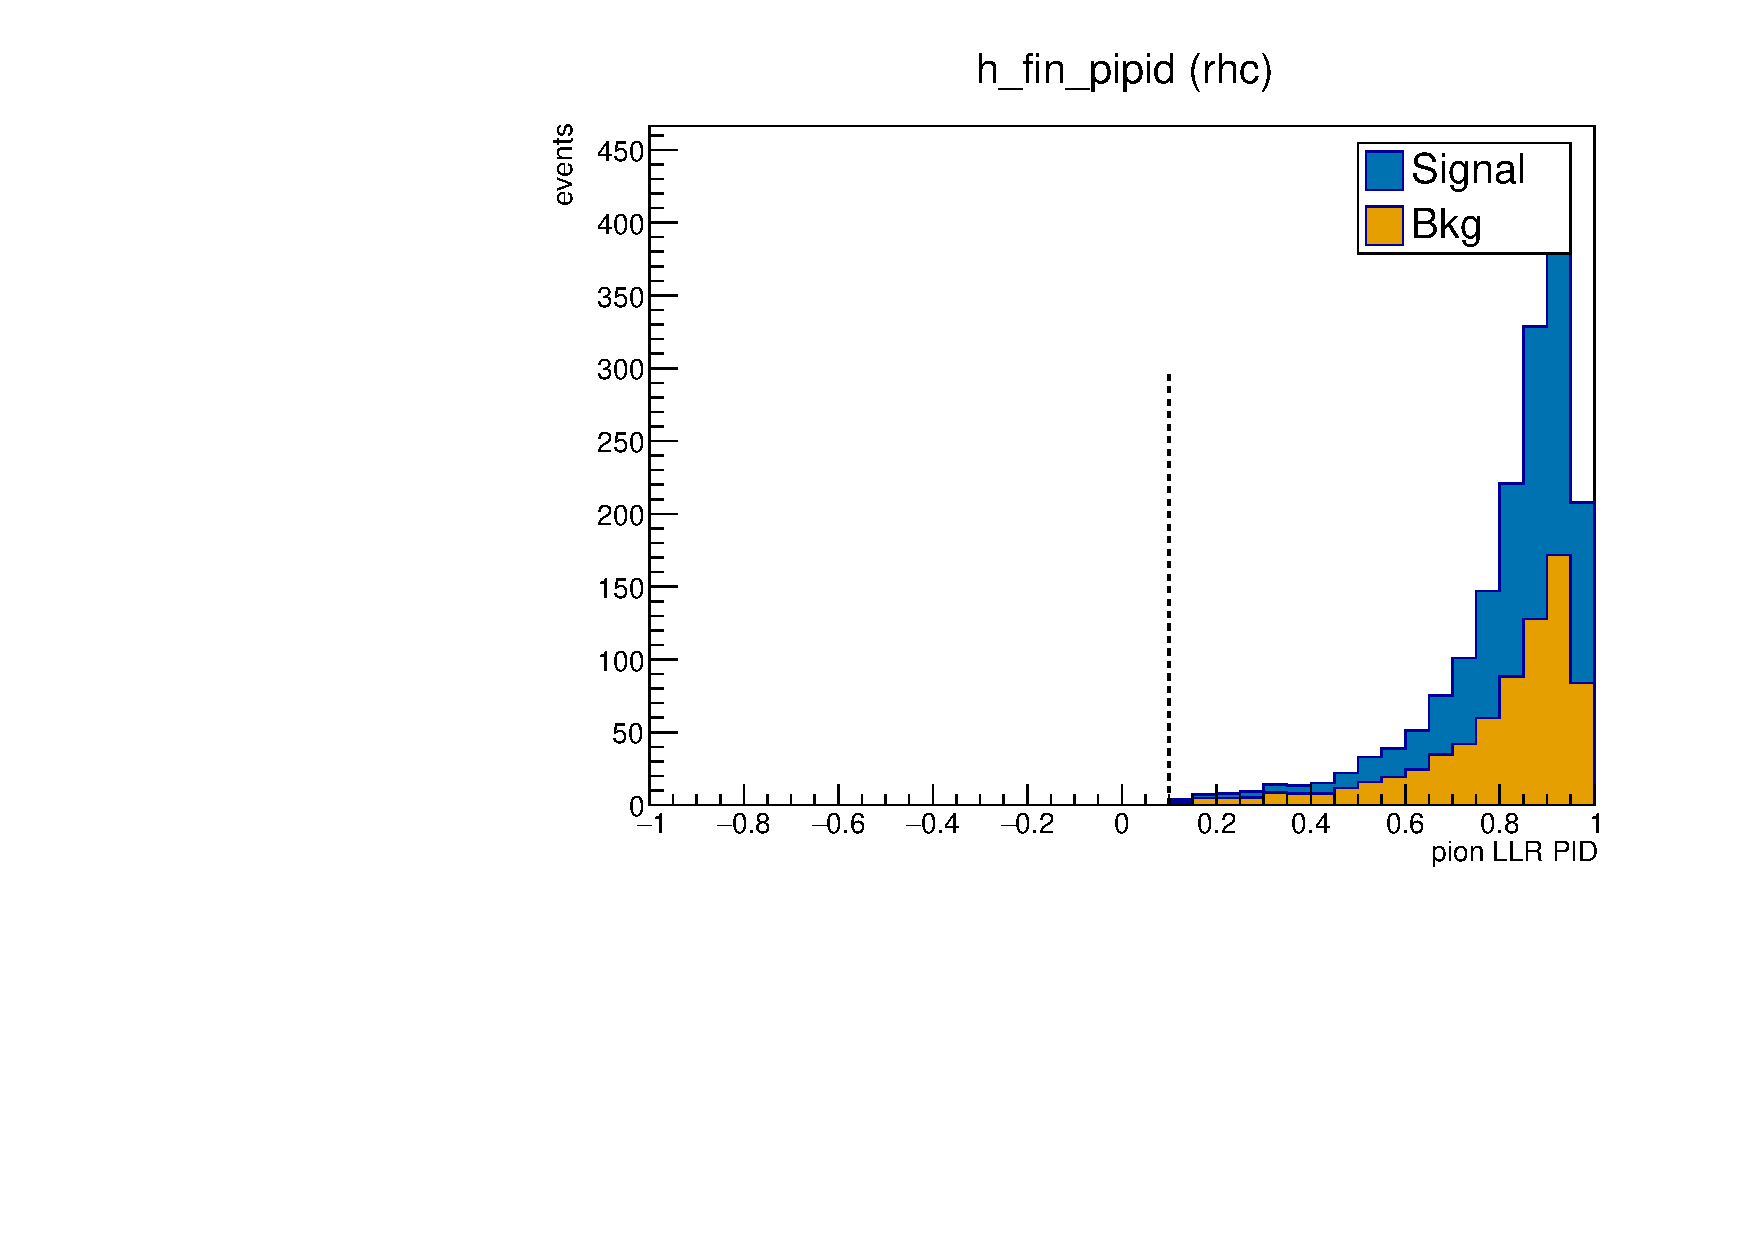
\includegraphics[width=\textwidth]{final_pipid_rhc}\caption{Pion LLR PID, RHC.}\end{subfigure}\hfill\\[6pt]
  \begin{subfigure}[b]{0.32\textwidth}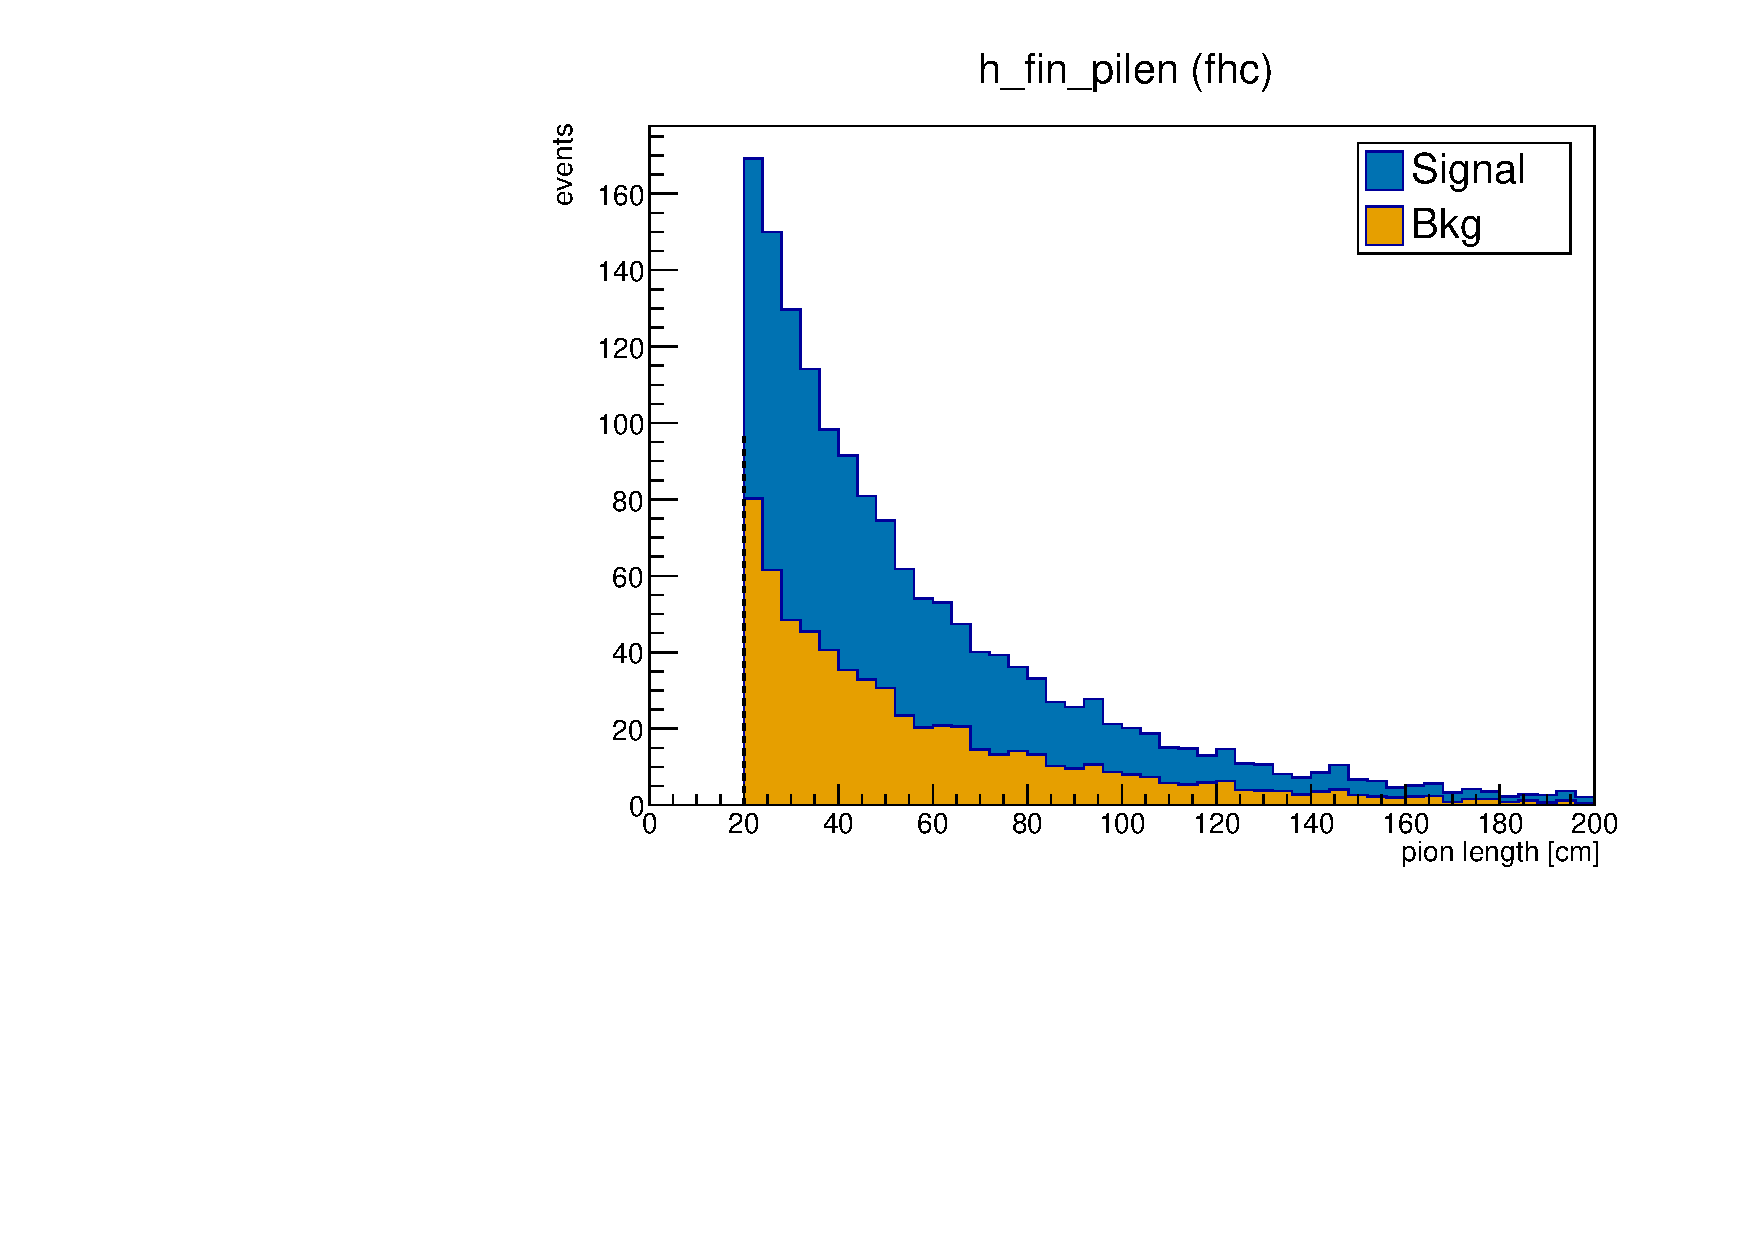
\includegraphics[width=\textwidth]{final_pilen_fhc}\caption{Pion length, FHC.}\end{subfigure}\hfill
  \begin{subfigure}[b]{0.32\textwidth}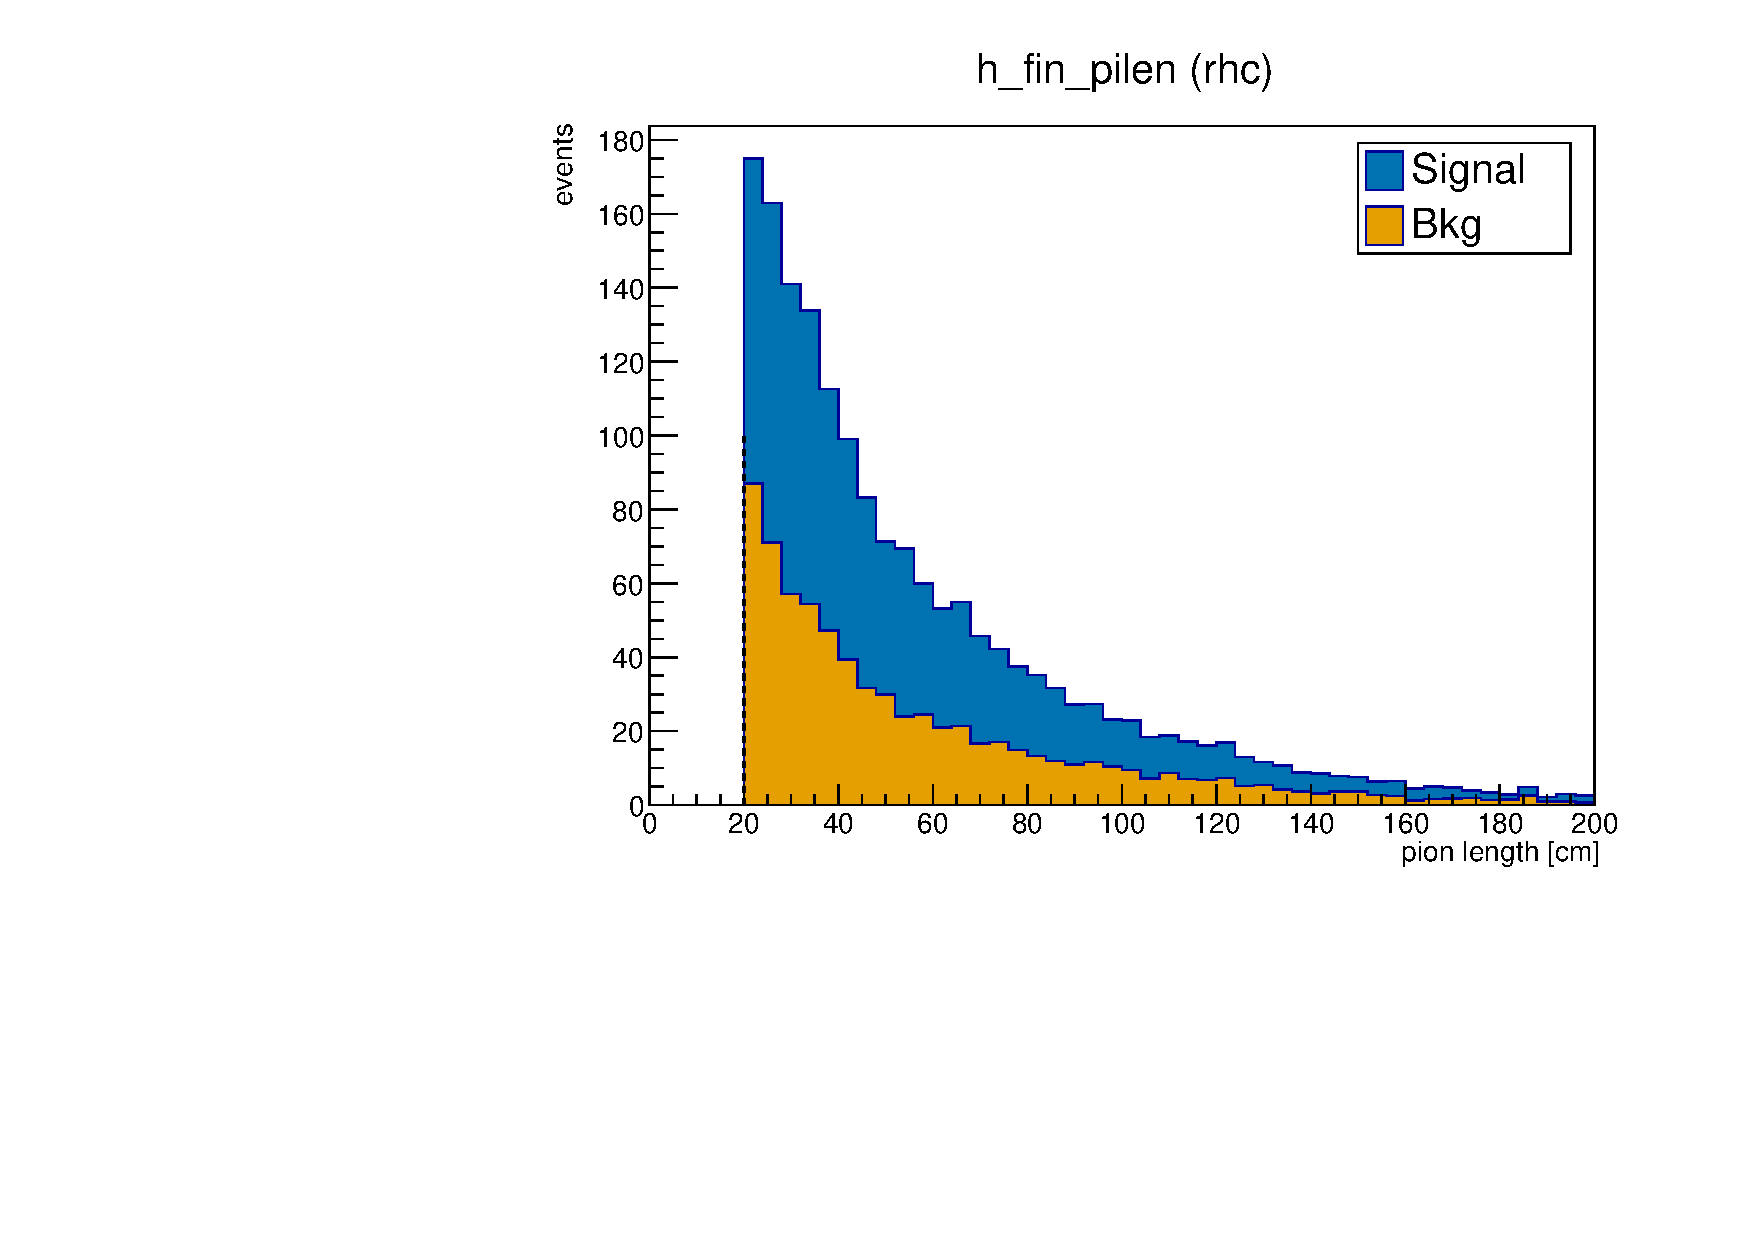
\includegraphics[width=\textwidth]{final_pilen_rhc}\caption{Pion length, RHC.}\end{subfigure}\hfill
  \caption{Pion-candidate LLR PID (top) and track length (bottom) at the final
    cut, for FHC and RHC (the combined configuration is consistent with both and is not
    shown). Signal (blue) / background (orange) stacked.}
  \label{fig:final_pi}
\end{figure}

\begin{figure}[H]
  \centering
  \begin{subfigure}[b]{0.48\textwidth}
    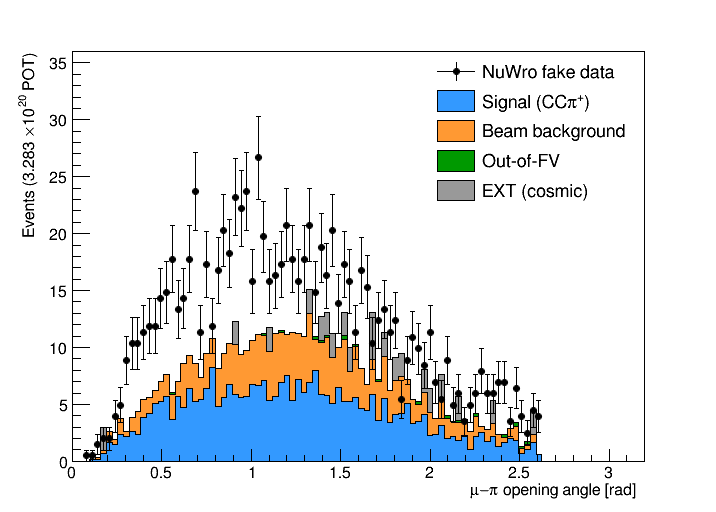
\includegraphics[width=\textwidth]{final_oa}
    \caption{$\mu$--$\pi$ opening angle.}
  \end{subfigure}
  \hfill
  \begin{subfigure}[b]{0.48\textwidth}
    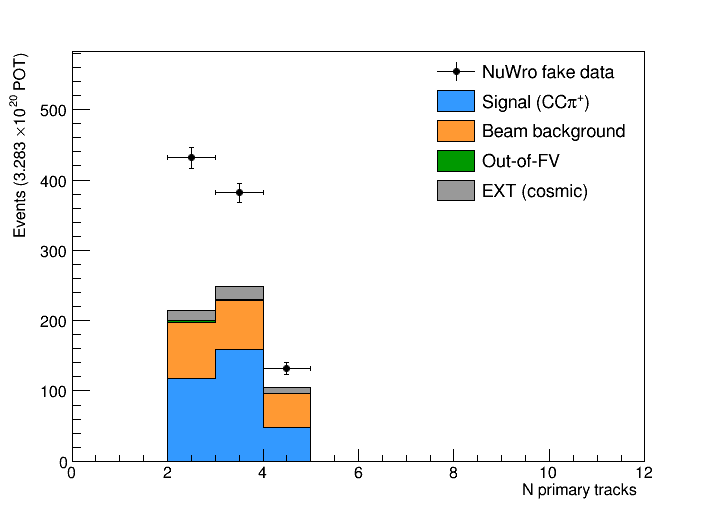
\includegraphics[width=\textwidth]{final_ntracks}
    \caption{Number of primary tracks.}
  \end{subfigure}
  \caption{Fake-data/MC comparison for topological variables at the final cut.}
  \label{fig:final_topo}
\end{figure}

\subsection{Background decomposition}

Table~\ref{tab:bkgcomp} shows the truth-level background breakdown at the final cut.

\begin{table}[H]
  \centering
  \caption{Background composition at the final cut, FHC full exposure (truth classes of
    the selection's counters, CV-weighted and per-run POT-scaled; the same classes and
    yields as the signal-region column of \suppref{Table}{tab:cr_transfer}). Fractions are of
    the $637$ neutrino-background events; beam-off and dirt are listed for scale.
   }
  \label{tab:bkgcomp}
  \begin{tabular}{lrr}
    \toprule
    Category & Events & Fraction \\
    \midrule
    $\nu_\mu$CC $0\pi$ (proton or other track as pion) & $244$ & $38\%$ \\
    $\nu_\mu$CC $\geq2\pi^\pm$, no $\pi^0$            & $145$ & $23\%$ \\
    NC and $\nu_e$CC                                  & $89.5$ & $14\%$ \\
    $\nu_\mu$CC with a $\pi^0$                        & $58.0$ & $9\%$ \\
    $\nu_\mu$CC $1\pi^\pm$ outside the measured phase space & $52.7$ & $8\%$ \\
    Out of fiducial volume                            & $47.4$ & $7\%$ \\
    EXT (cosmic)                                      & $30$ & n/a \\
    Dirt                                              & $1.3$ & n/a \\
    \bottomrule
  \end{tabular}
\end{table}

The dominant background ($38\%$) is CC0$\pi$ interactions in which a proton
is reconstructed as the pion candidate.  This mis-identification was verified
directly by 2D event displays (truth-labelled by backtracked PDG): the pion candidate
track shows a green (proton) truth colour with a stopping Bragg peak, while the
genuine muon track is correctly identified.

At the current working point (Bragg-pion score $\geq 0.08$), the pion
candidate is truth-matched to a proton in $\approx18\%$ of cases.  Tighter
Bragg-score thresholds (0.20--0.30) were studied but shown not to improve the
figure of merit: the pion-to-proton ratio in CC$\pi^{\pm}$ signal is $\approx4:1$,
so rejecting protons removes genuine pions at nearly the same rate.

\subsection{Event displays}

Figure~\ref{fig:evdisp} shows representative 2D truth-labelled event displays
for the two dominant backgrounds and the EXT cosmic sample.  Tracks are coloured
by backtracked truth PDG: $\mu$ (blue), $\pi^\pm$ (red), $p$ (green),
cosmic/unmatched (grey).  The muon candidate is drawn solid-thick; the pion
candidate dashed-thick; the reconstructed $\nu$ vertex is shown as a star.

\begin{figure}[H]
  \centering
  \begin{subfigure}[b]{0.32\textwidth}
    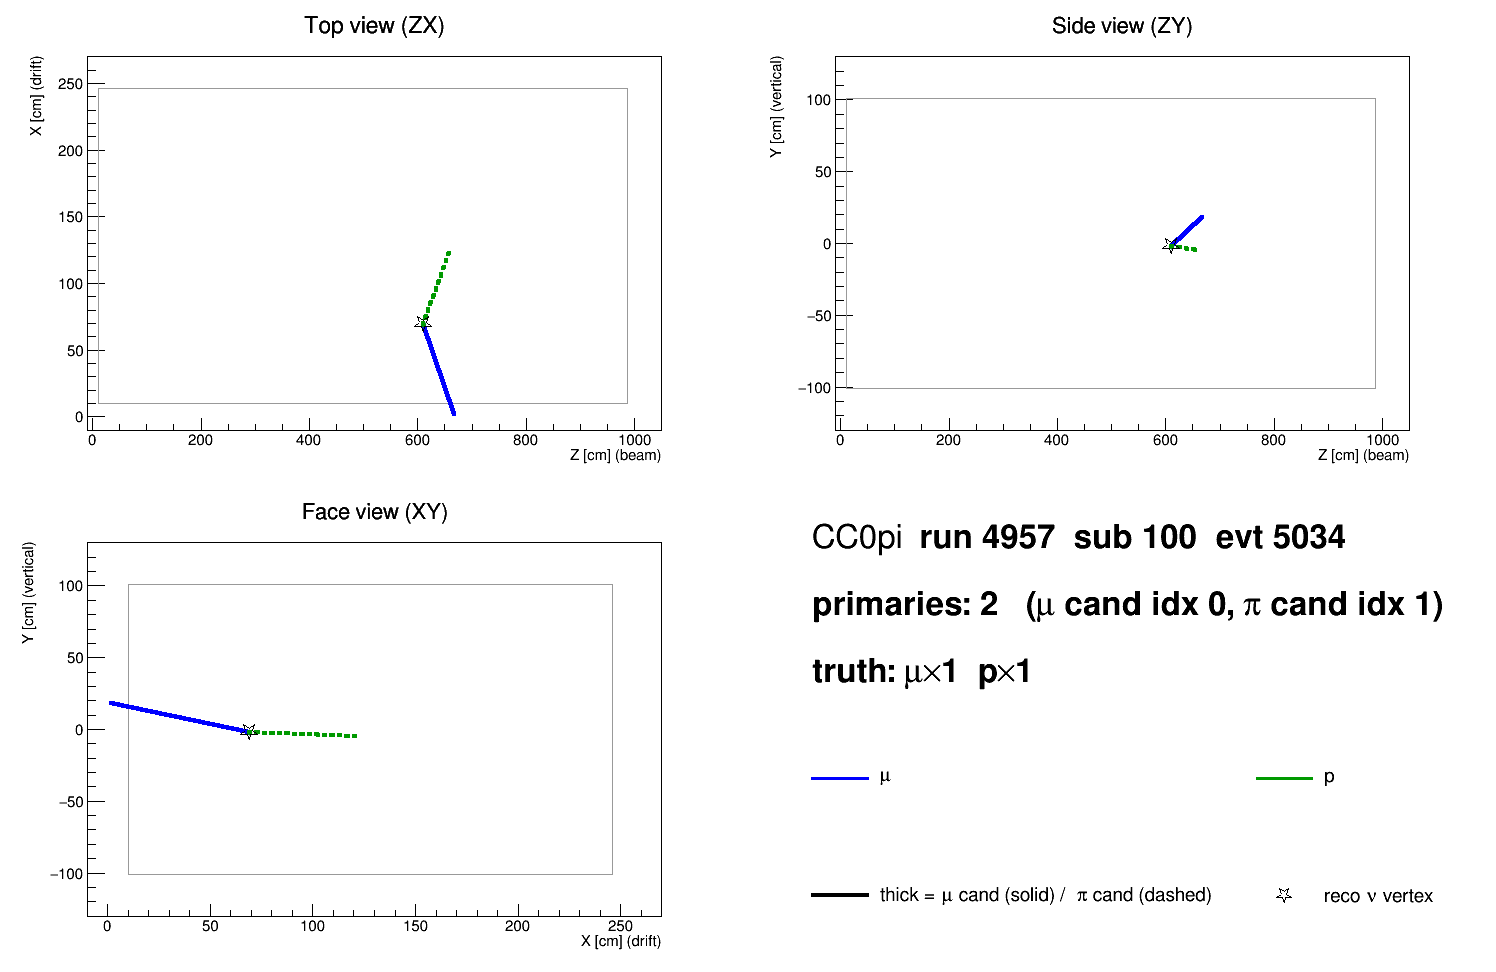
\includegraphics[width=\textwidth]{evdisp_cc0pi}
    \caption{CC0$\pi$ background: a proton (green, dashed) is reconstructed
      as the pion candidate.}
  \end{subfigure}
  \hfill
  \begin{subfigure}[b]{0.32\textwidth}
    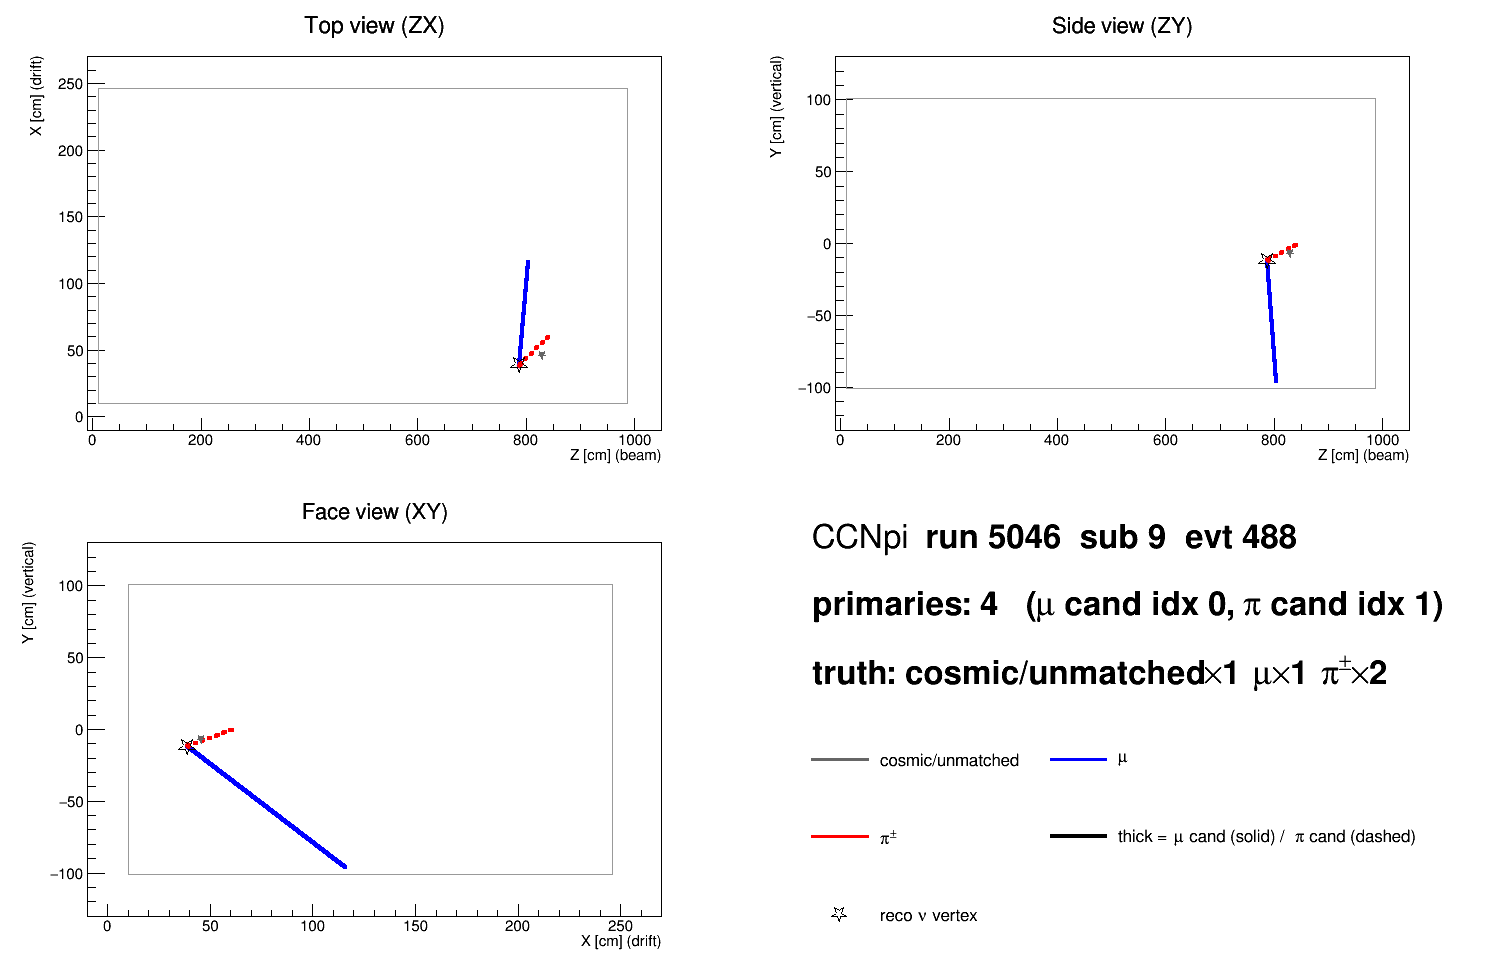
\includegraphics[width=\textwidth]{evdisp_ccnpi}
    \caption{CC$N\pi$ background: two genuine charged pions present; one
      is selected as the pion candidate.}
  \end{subfigure}
  \hfill
  \begin{subfigure}[b]{0.32\textwidth}
    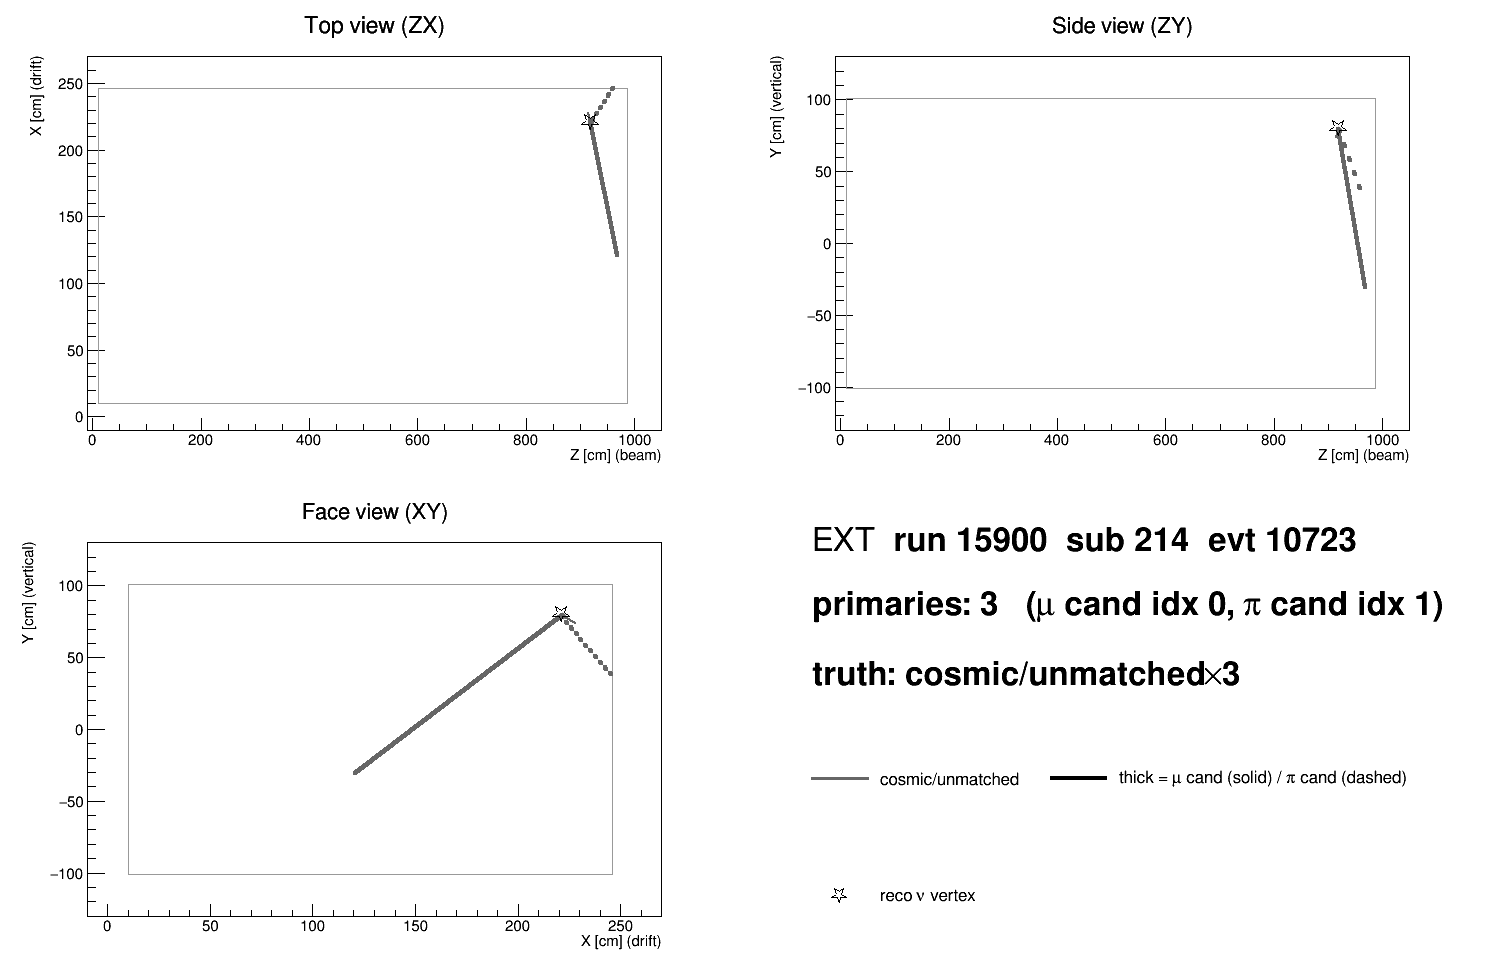
\includegraphics[width=\textwidth]{evdisp_ext}
    \caption{EXT cosmic event: all tracks are grey (no truth match), faking
      a neutrino vertex topology.}
  \end{subfigure}
  \caption{Truth-labelled 2D event displays (ZX projection) for representative
    background events at the final cut.  Three views (ZX top, ZY side, XY face)
    are generated per event.}
  \label{fig:evdisp}
\end{figure}

% =============================================================================
\section{Unfolding}
\label{sec:unfolding}
% =============================================================================

\subsection{The extraction chain, stage by stage}
\label{sec:chain}

Before the formalism, it is useful to see the measurement assembled in the order it is
actually performed. Each stage is shown for all three beam configurations in the flat
reco-bin space in which the unfolding operates (every analysis slice concatenated).

\paragraph{Stage 1, selected events, POT-scaled (Fig.~\ref{fig:chain_reco}).}
The starting point is the selected reconstructed spectrum, scaled to the full exposure of
each configuration with the per-run POT factors of \S\ref{sec:mc}. The Monte Carlo is
split into signal and background. At the final cut the purity is $\simeq59\%$
(Table~\ref{tab:cutflow}), so some $40\%$ of the selected events have to be removed
before anything can be interpreted as a signal rate. Because the analysis is blind, the
points are the Poisson-thrown fake data rather than beam-on data.

\paragraph{Stage 2, background subtraction (Fig.~\ref{fig:chain_bsub}).}
The estimated background is subtracted bin by bin, leaving the background-subtracted data
alongside the central-value MC signal. The neutrino background is taken from the
simulation, the cosmic component from beam-off (EXT) data, and the dirt component from the
dedicated overlay; the four control regions of \S\ref{sec:sidebands} are what validate
this step. This subtracted spectrum, not the raw selection, is the input to the unfolding.

\paragraph{Stage 3, unfolding.}
The subtracted spectrum still folds in the detector response and the selection efficiency,
encoded in the response matrix of \S\ref{sec:unfolding_resp}. With $50$--$99\%$ bin migration a
direct inversion is unusable (\S\ref{sec:unfmethods}), so the measurement is
regularised with Wiener--SVD. The price is the additional-smearing matrix $A_C$: what is
recovered is $A_C\times$(true signal), and \emph{every} model must therefore be multiplied
by $A_C$ before being compared with the data.

\paragraph{Stage 4, comparison with models.}
The unfolded result is then compared with the MicroBooNE tune and the four external
generators, all $A_C$-smeared into the same space (\S\ref{sec:rhc}). It is worth
separating two effects that are easily conflated. $A_C$ suppresses the integral of each
prediction, but it does so by a \emph{common} factor: for FHC $p_\mu$ it is $0.78$, $0.78$,
$0.76$ and $0.79$ for GENIE, GiBUU, NEUT and NuWro respectively (smeared integral over
truth-level total, from the released curves). The truth-level totals of
those same generators span $0.82$ to $1.32\times10^{-38}$~cm$^2$/Ar (\suppref{Table}{tab:total_xsec}), a factor $1.6$. A
common $\simeq\!0.78$ factor cannot produce a $1.6\times$ spread, so the differences between
the generators are genuine model differences and not an artefact of the regularisation.
The one-bin total of \S\ref{sec:total_xsec} provides the independent check,
since with a single bin there is no regularisation and $A_C\equiv1$.

\begin{figure}[H]
  \centering
  \begin{subfigure}[b]{0.32\textwidth}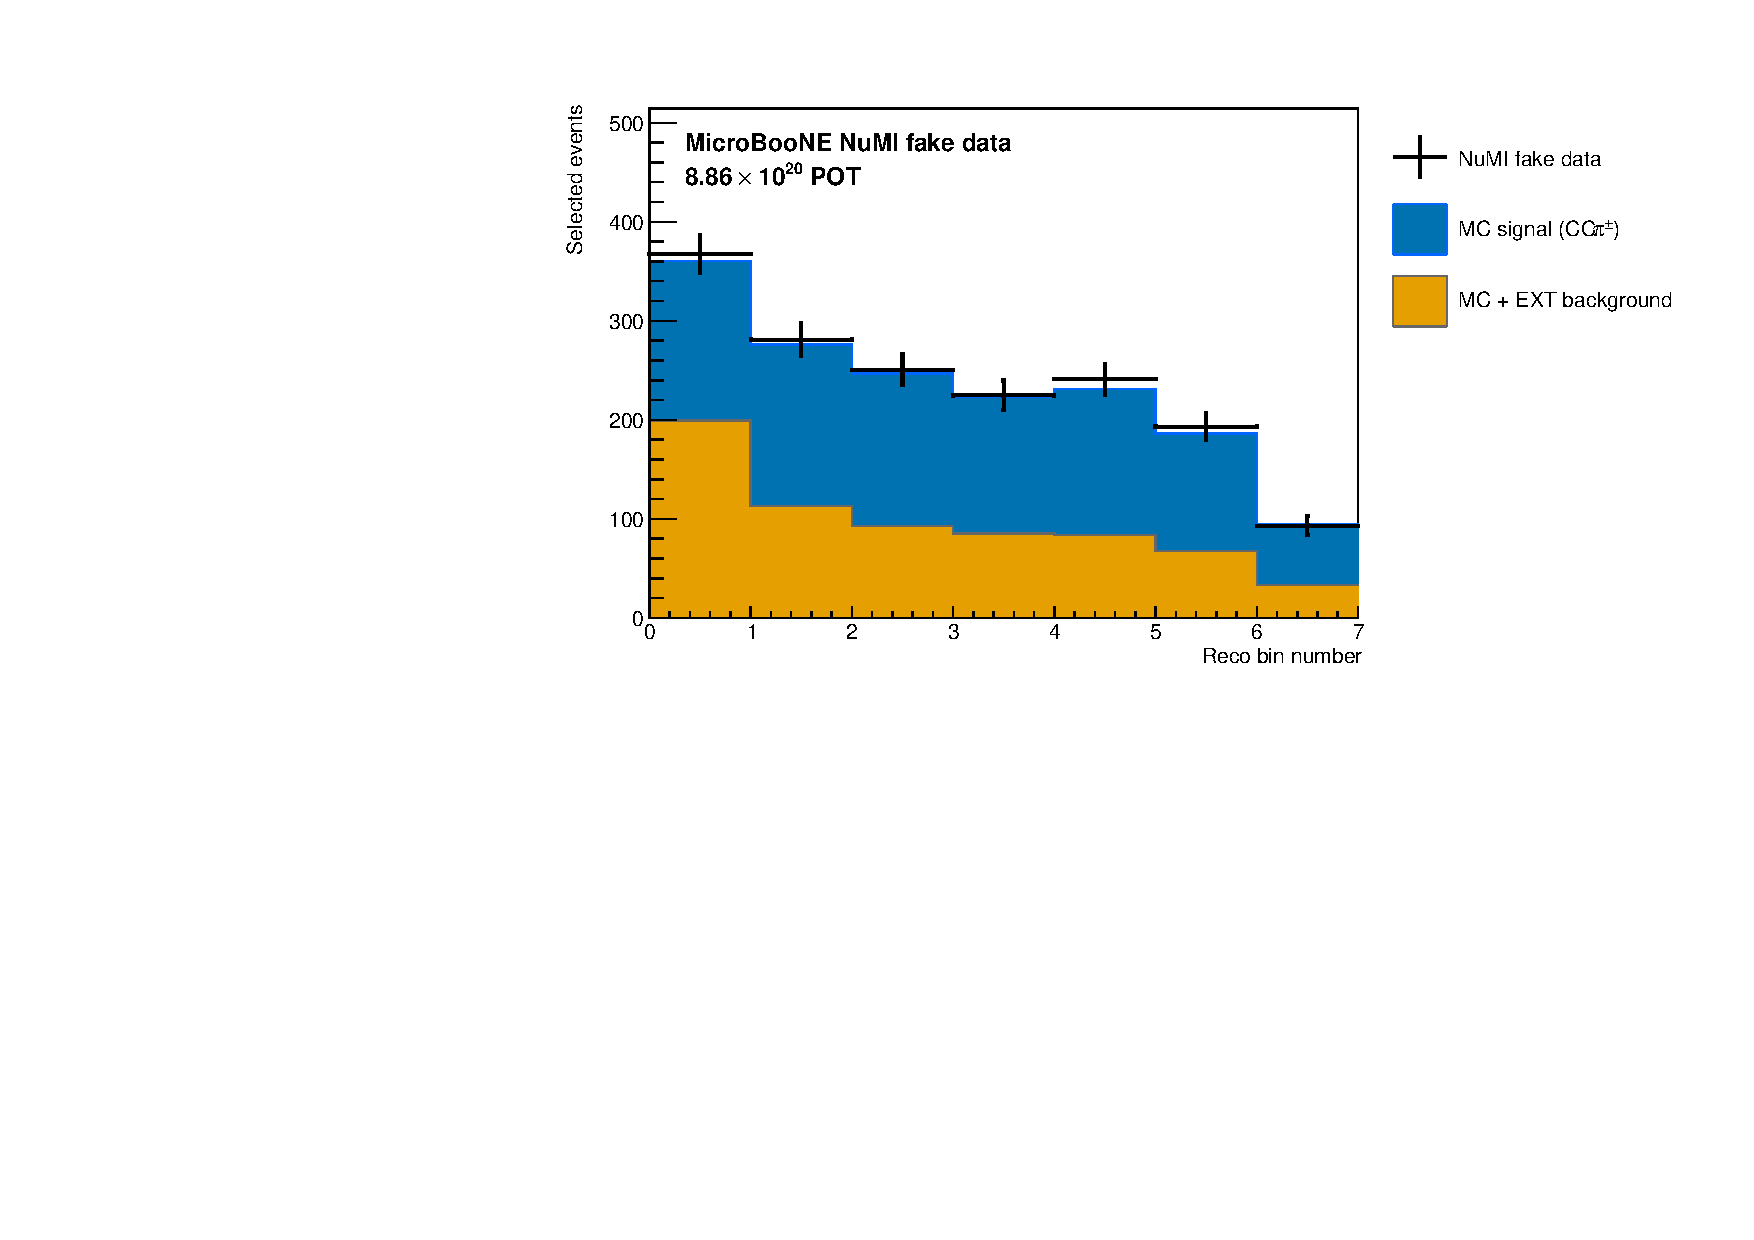
\includegraphics[width=\textwidth]{step1_reco_pmu}\caption{$p_\mu$}\end{subfigure}\hfill
  \begin{subfigure}[b]{0.32\textwidth}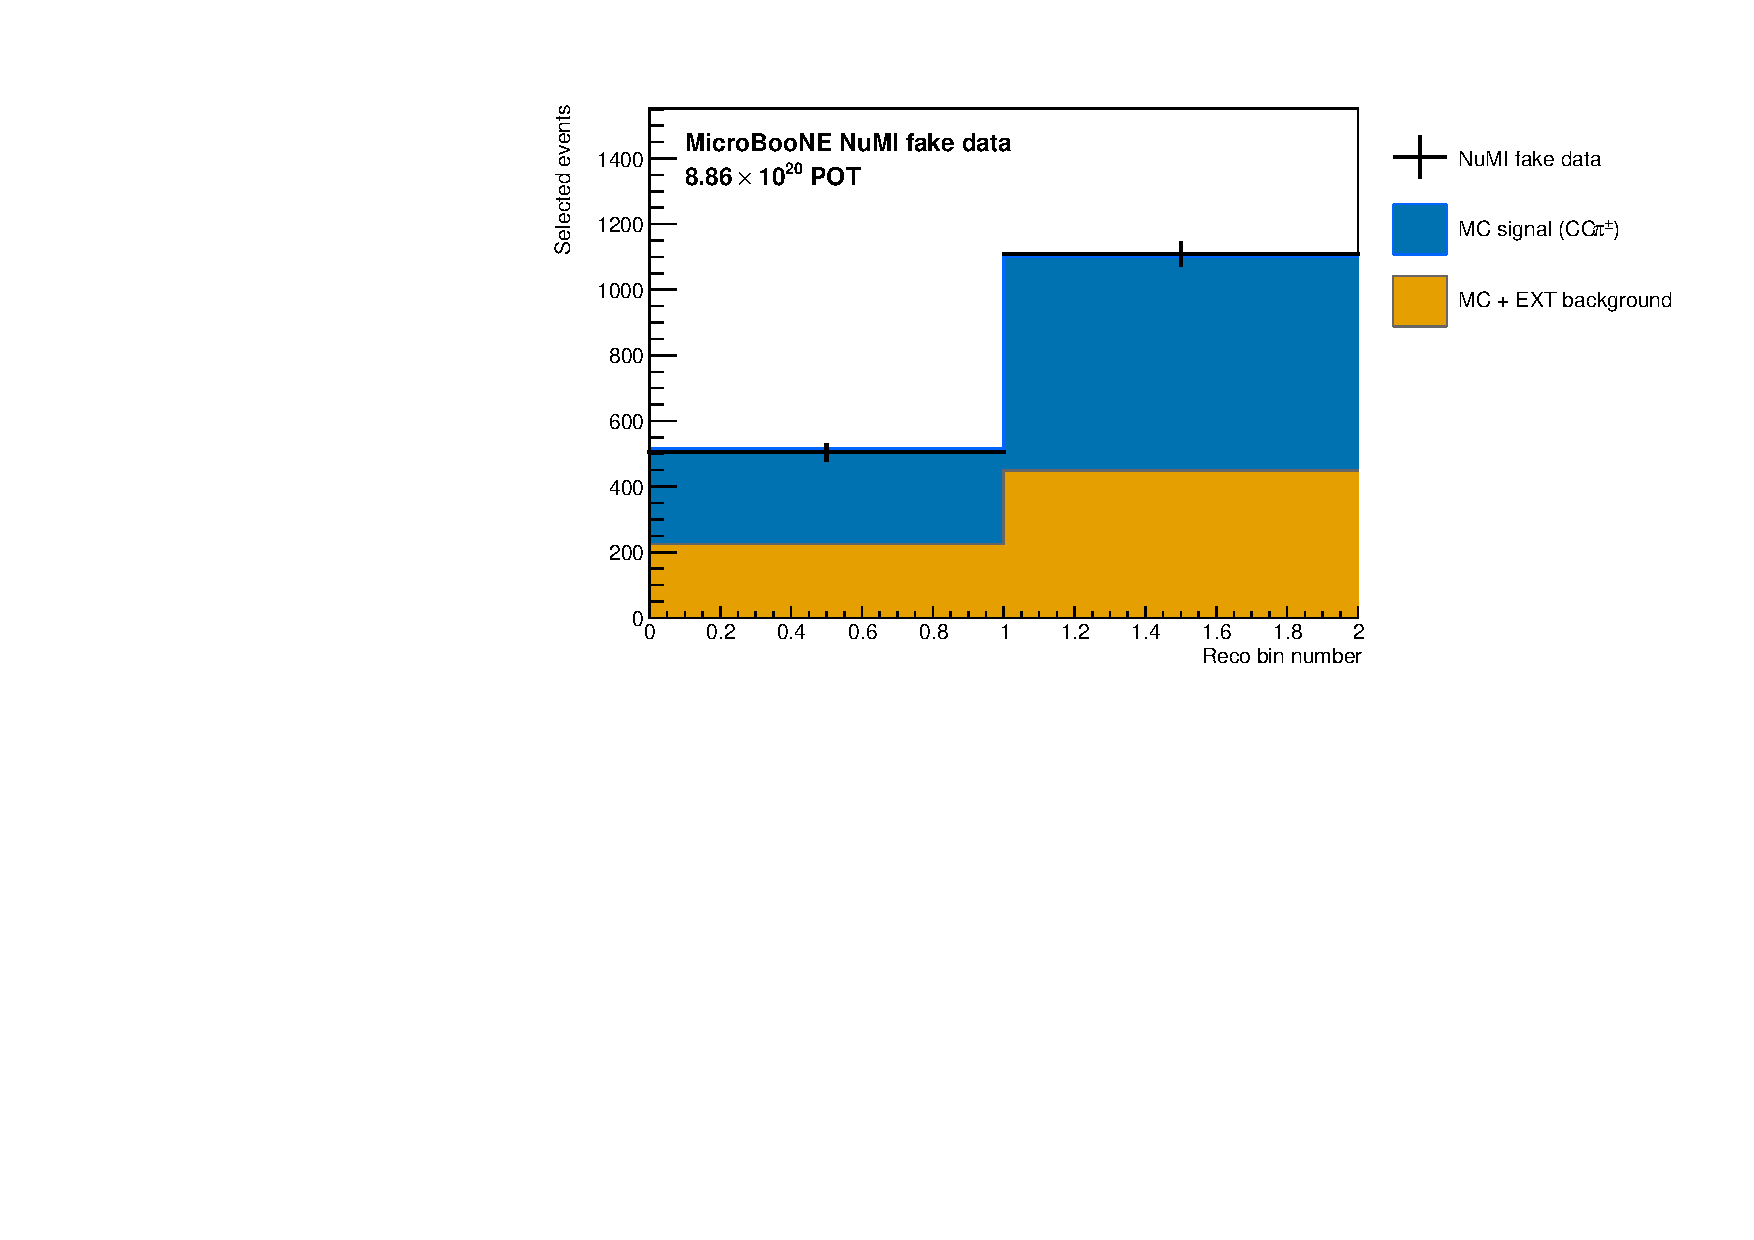
\includegraphics[width=\textwidth]{step1_reco_ppi}\caption{$p_\pi$}\end{subfigure}\hfill
  \begin{subfigure}[b]{0.32\textwidth}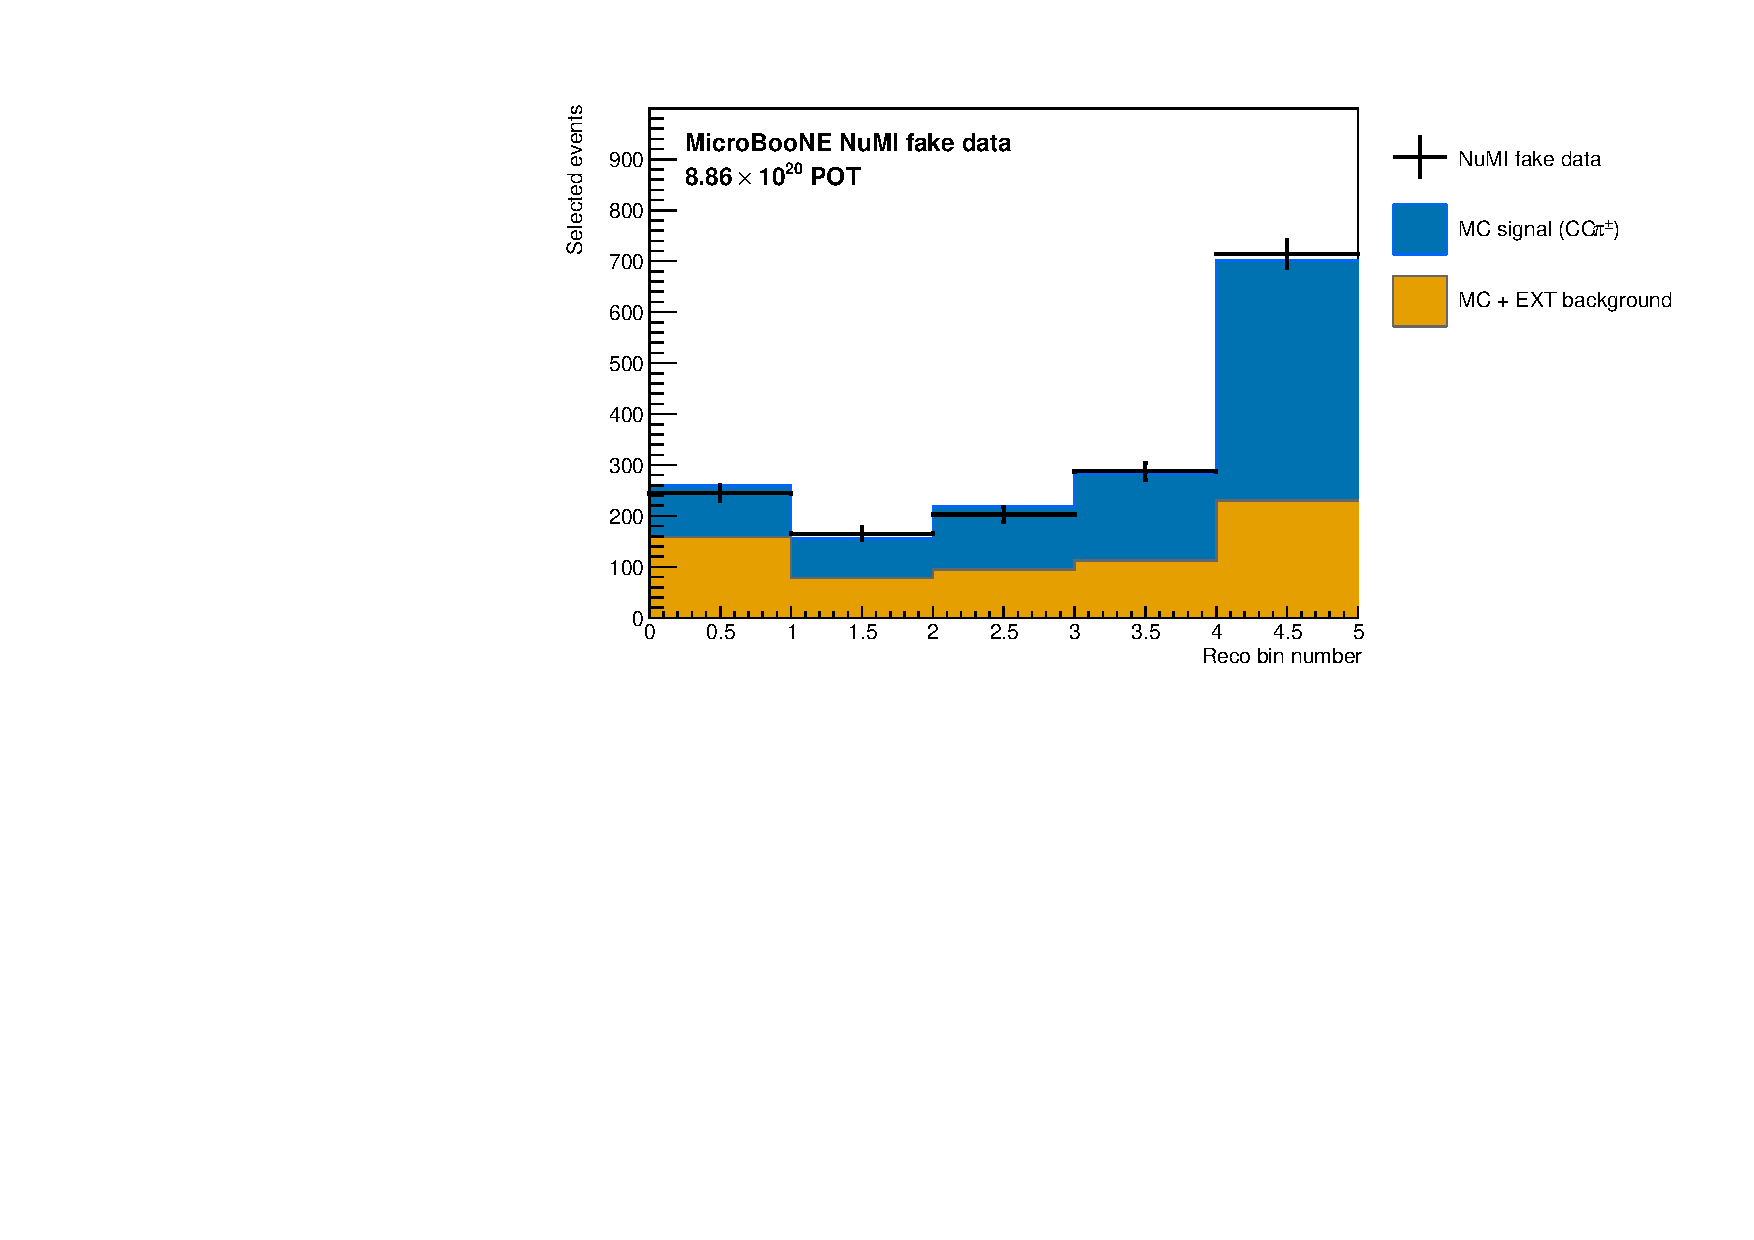
\includegraphics[width=\textwidth]{step1_reco_costhmu}\caption{$\cos\theta_\mu$}\end{subfigure}

  \vspace{3mm}
  \begin{subfigure}[b]{0.32\textwidth}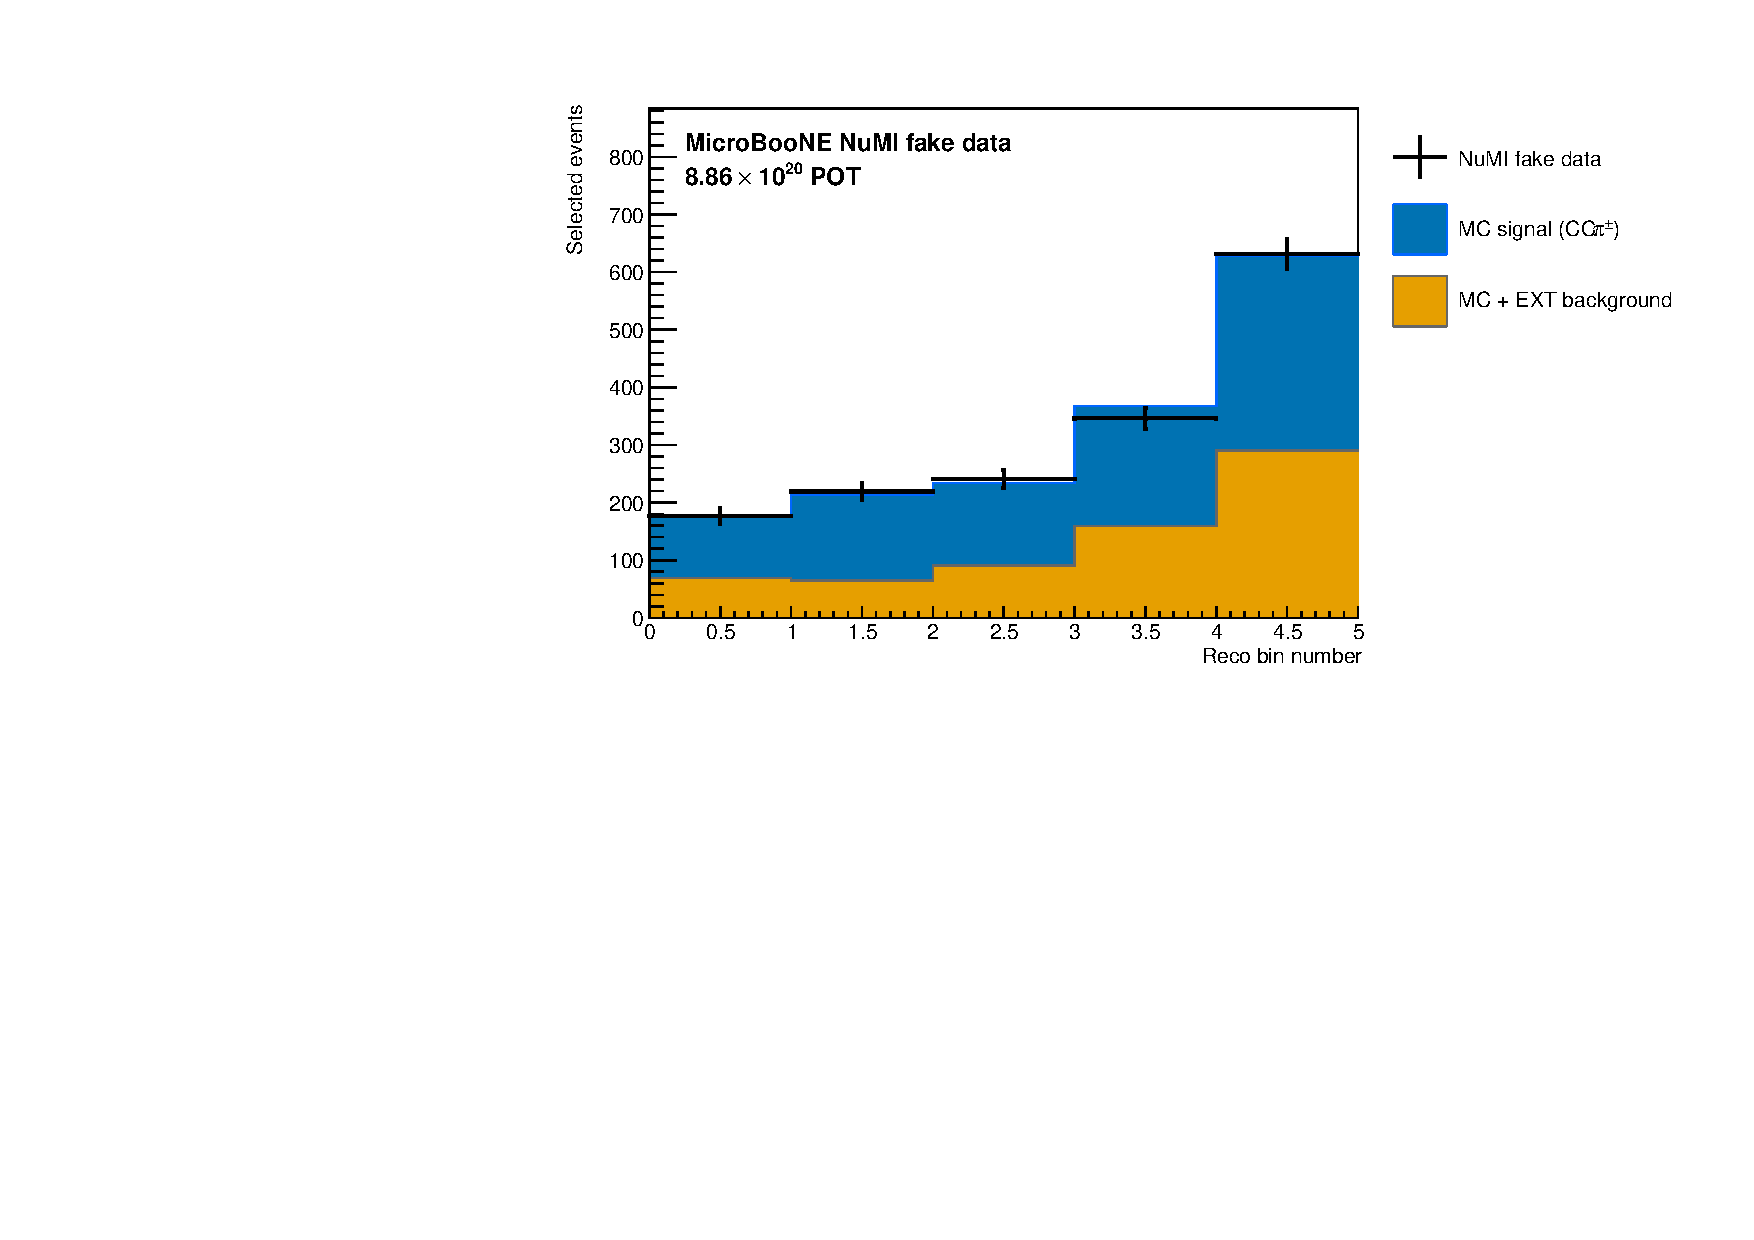
\includegraphics[width=\textwidth]{step1_reco_costhpi}\caption{$\cos\theta_\pi$}\end{subfigure}\hfill
  \begin{subfigure}[b]{0.32\textwidth}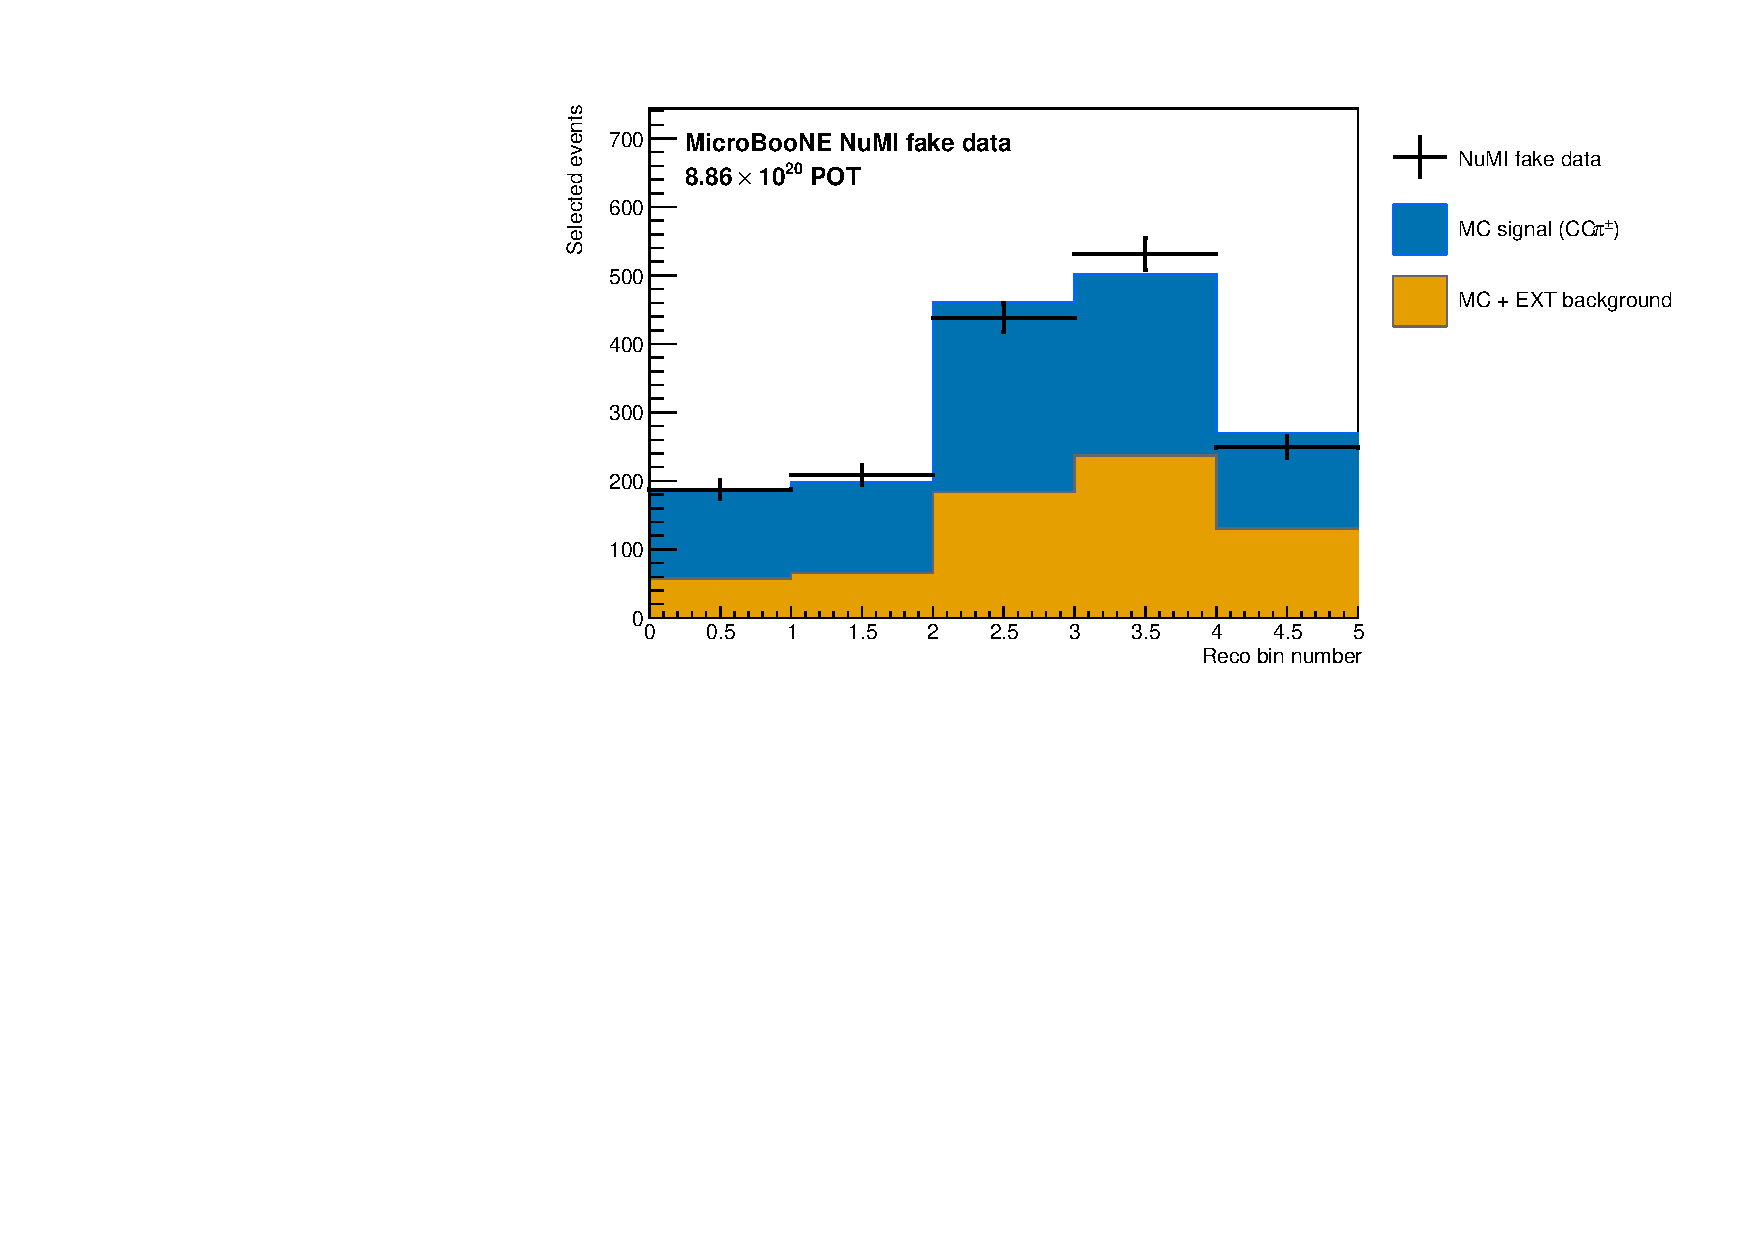
\includegraphics[width=\textwidth]{step1_reco_thmupi}\caption{$\theta_{\mu\pi}$}\end{subfigure}\hfill
  \begin{subfigure}[b]{0.32\textwidth}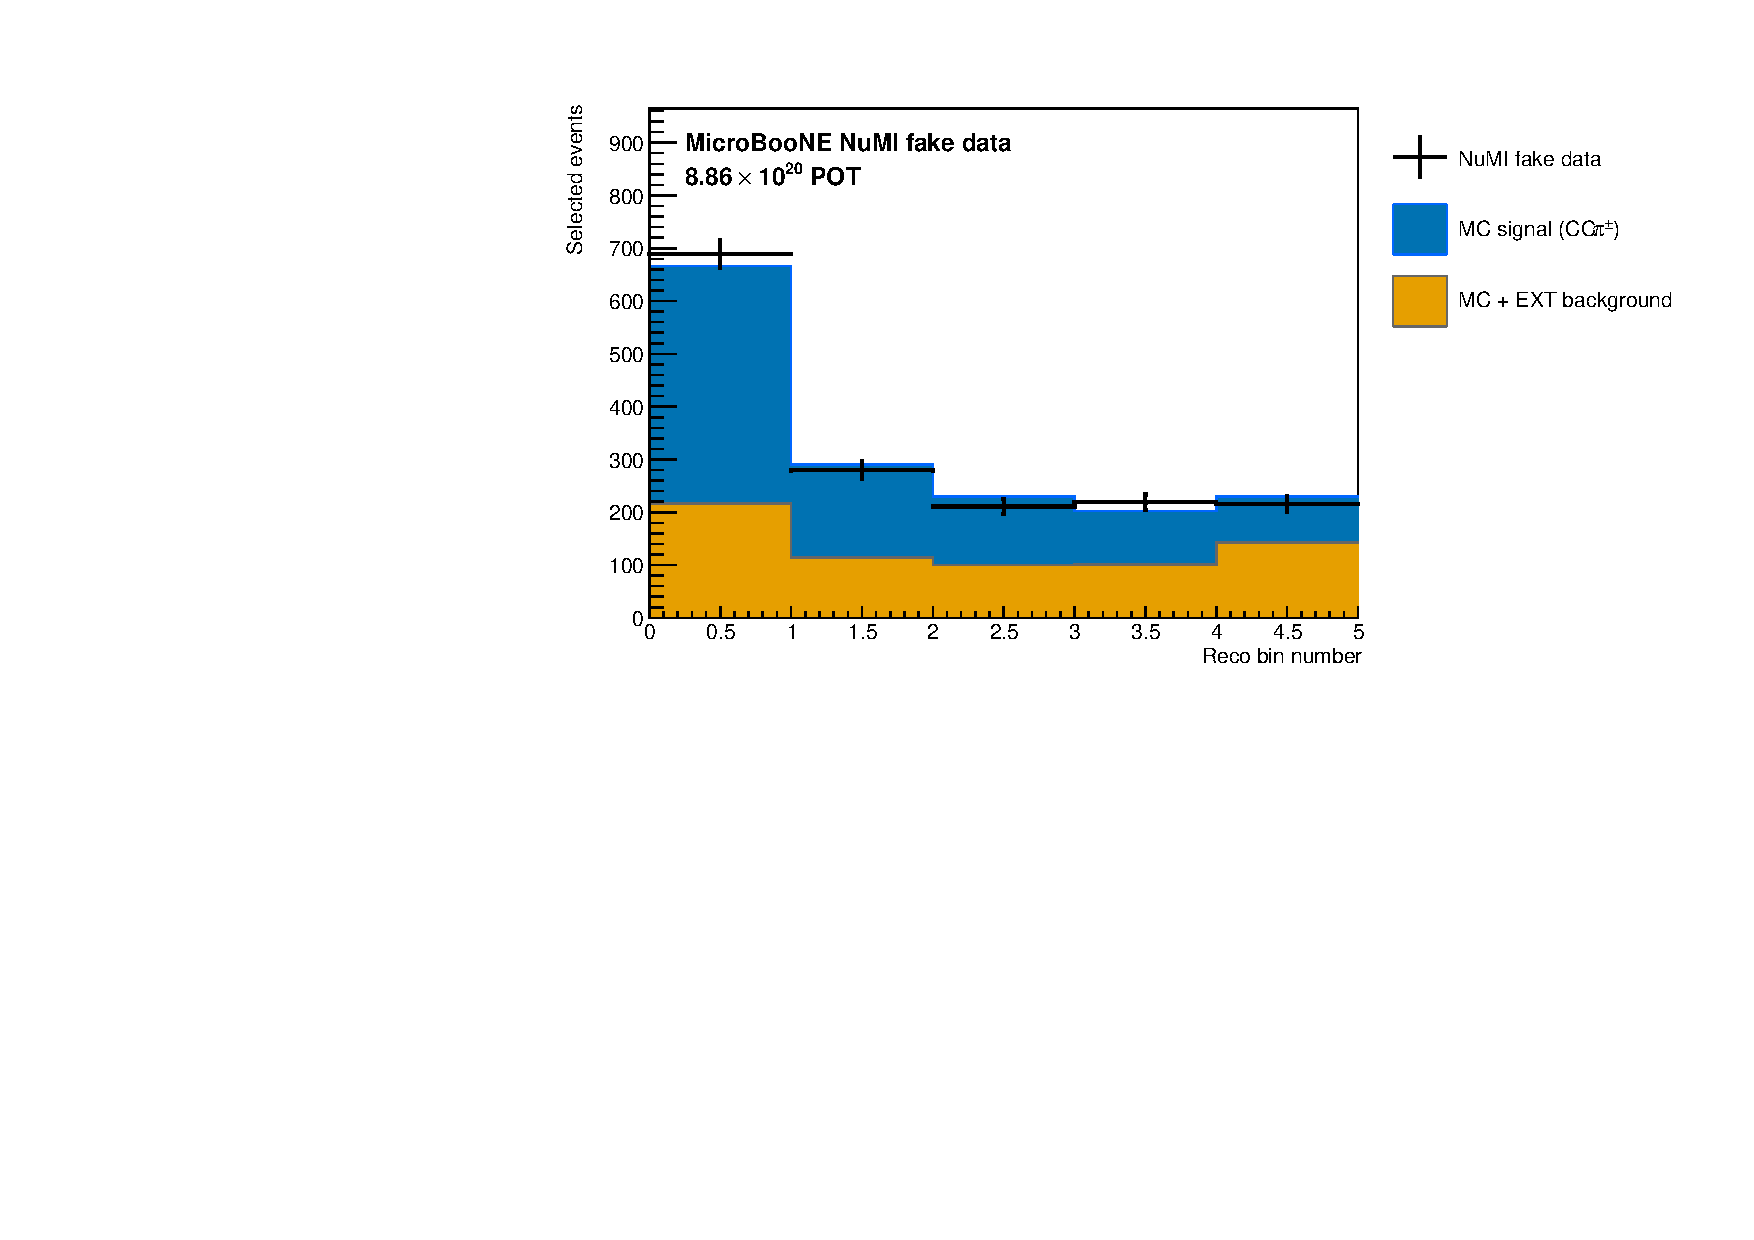
\includegraphics[width=\textwidth]{step1_reco_thetamu}\caption{$\theta_\mu$}\end{subfigure}
  \caption{Stage 1, FHC: selected reconstructed spectra scaled to the full exposure, with
    the MC split into signal and background. Points are the Poisson-thrown fake data.
    The RHC and combined equivalents are Figs.~\ref{fig:chain_reco_rhc}
    (the combined configuration is in \suppref{Fig.}{fig:chain_reco_comb}).}
  \label{fig:chain_reco}
\end{figure}

\begin{figure}[H]
  \centering
  \begin{subfigure}[b]{0.32\textwidth}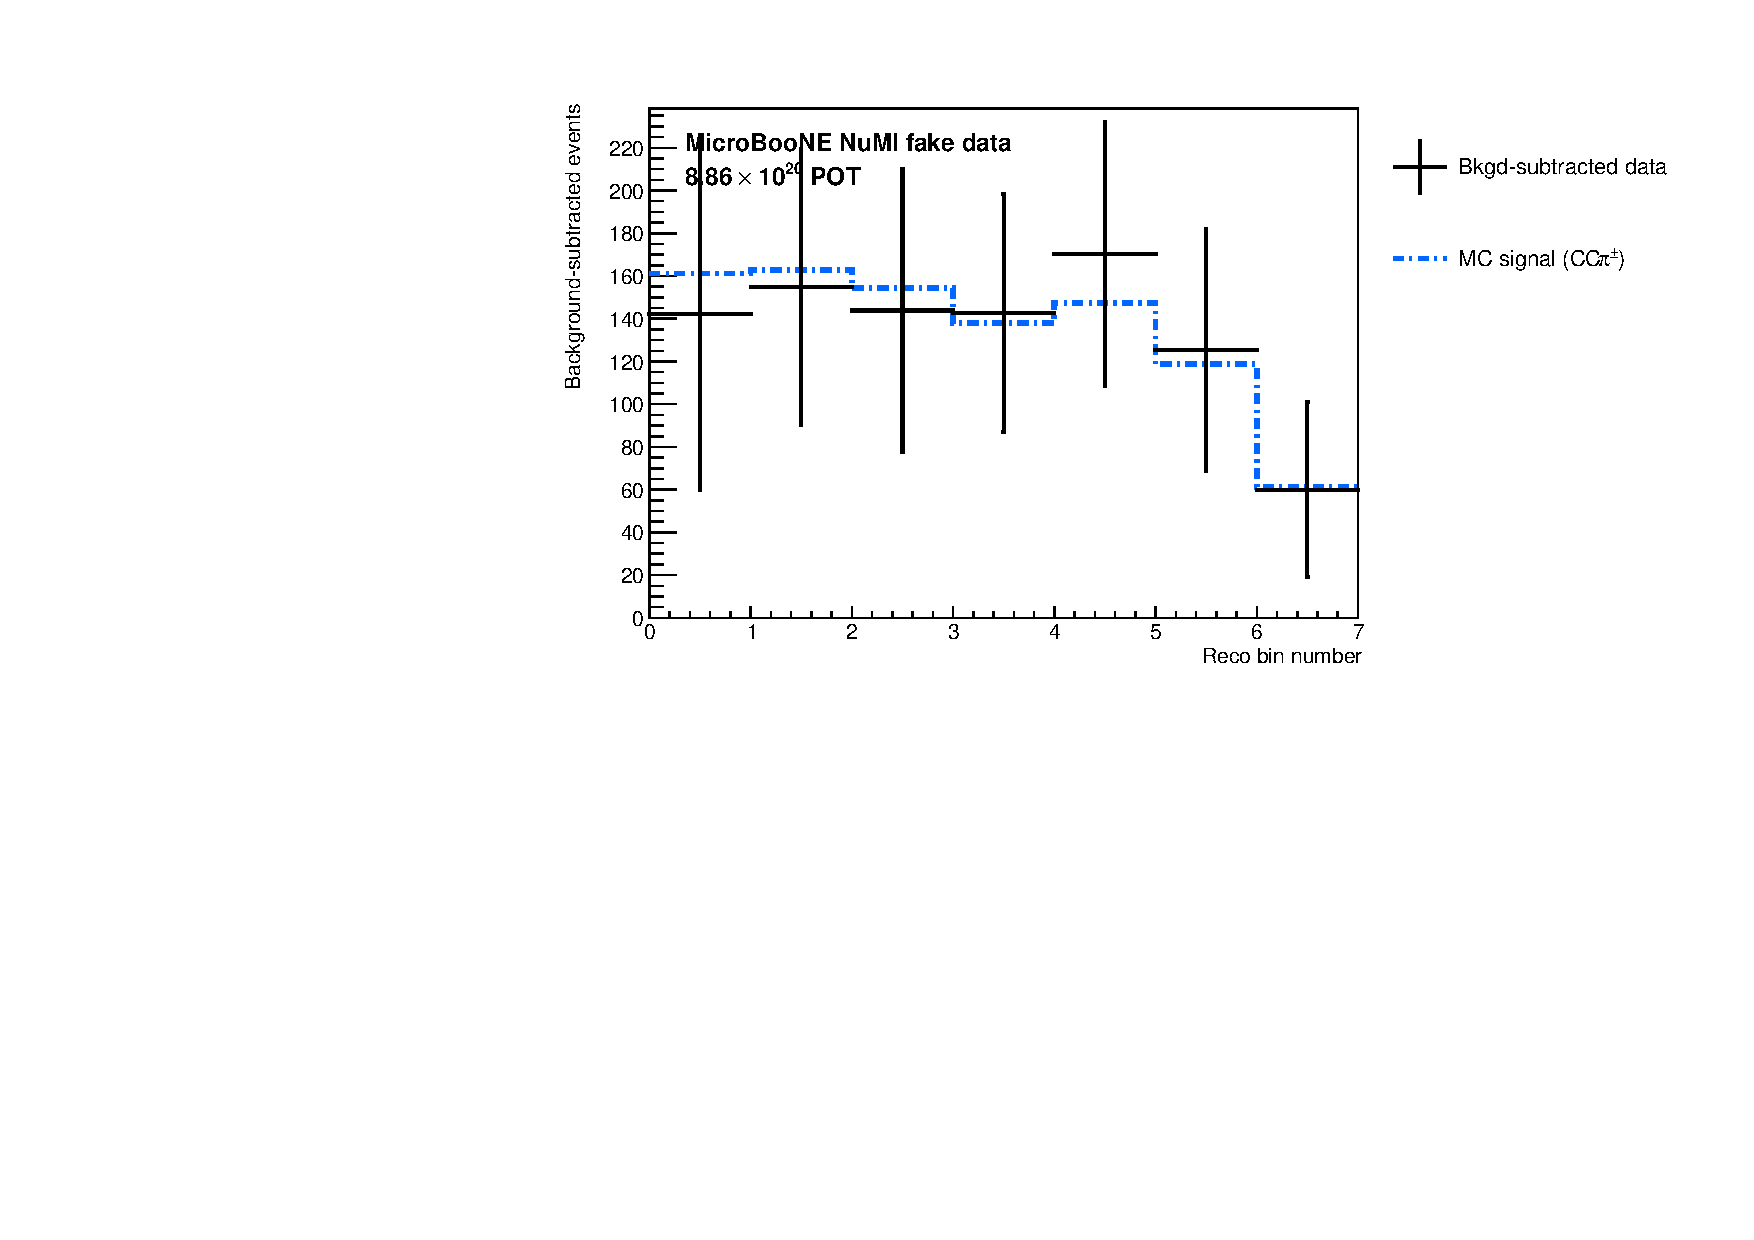
\includegraphics[width=\textwidth]{step2_bsub_pmu}\caption{$p_\mu$}\end{subfigure}\hfill
  \begin{subfigure}[b]{0.32\textwidth}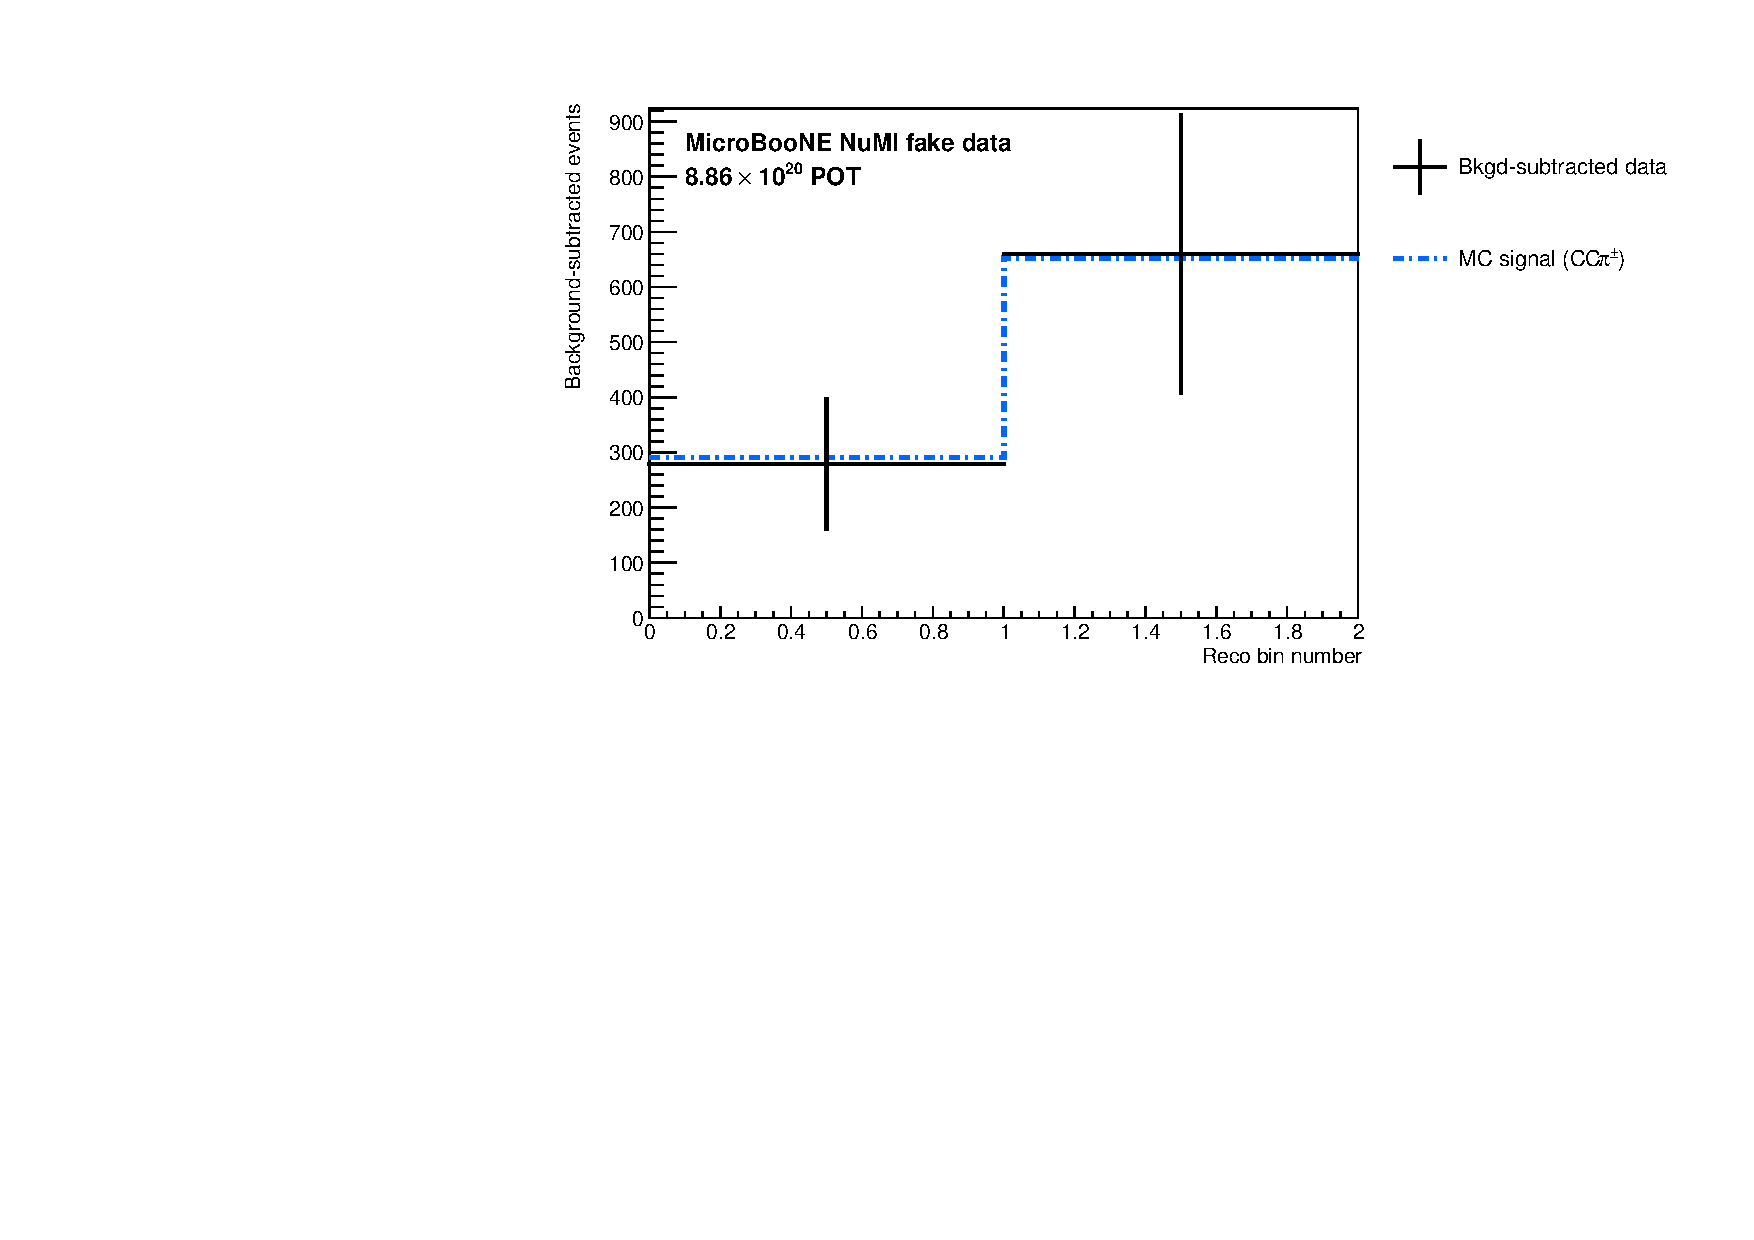
\includegraphics[width=\textwidth]{step2_bsub_ppi}\caption{$p_\pi$}\end{subfigure}\hfill
  \begin{subfigure}[b]{0.32\textwidth}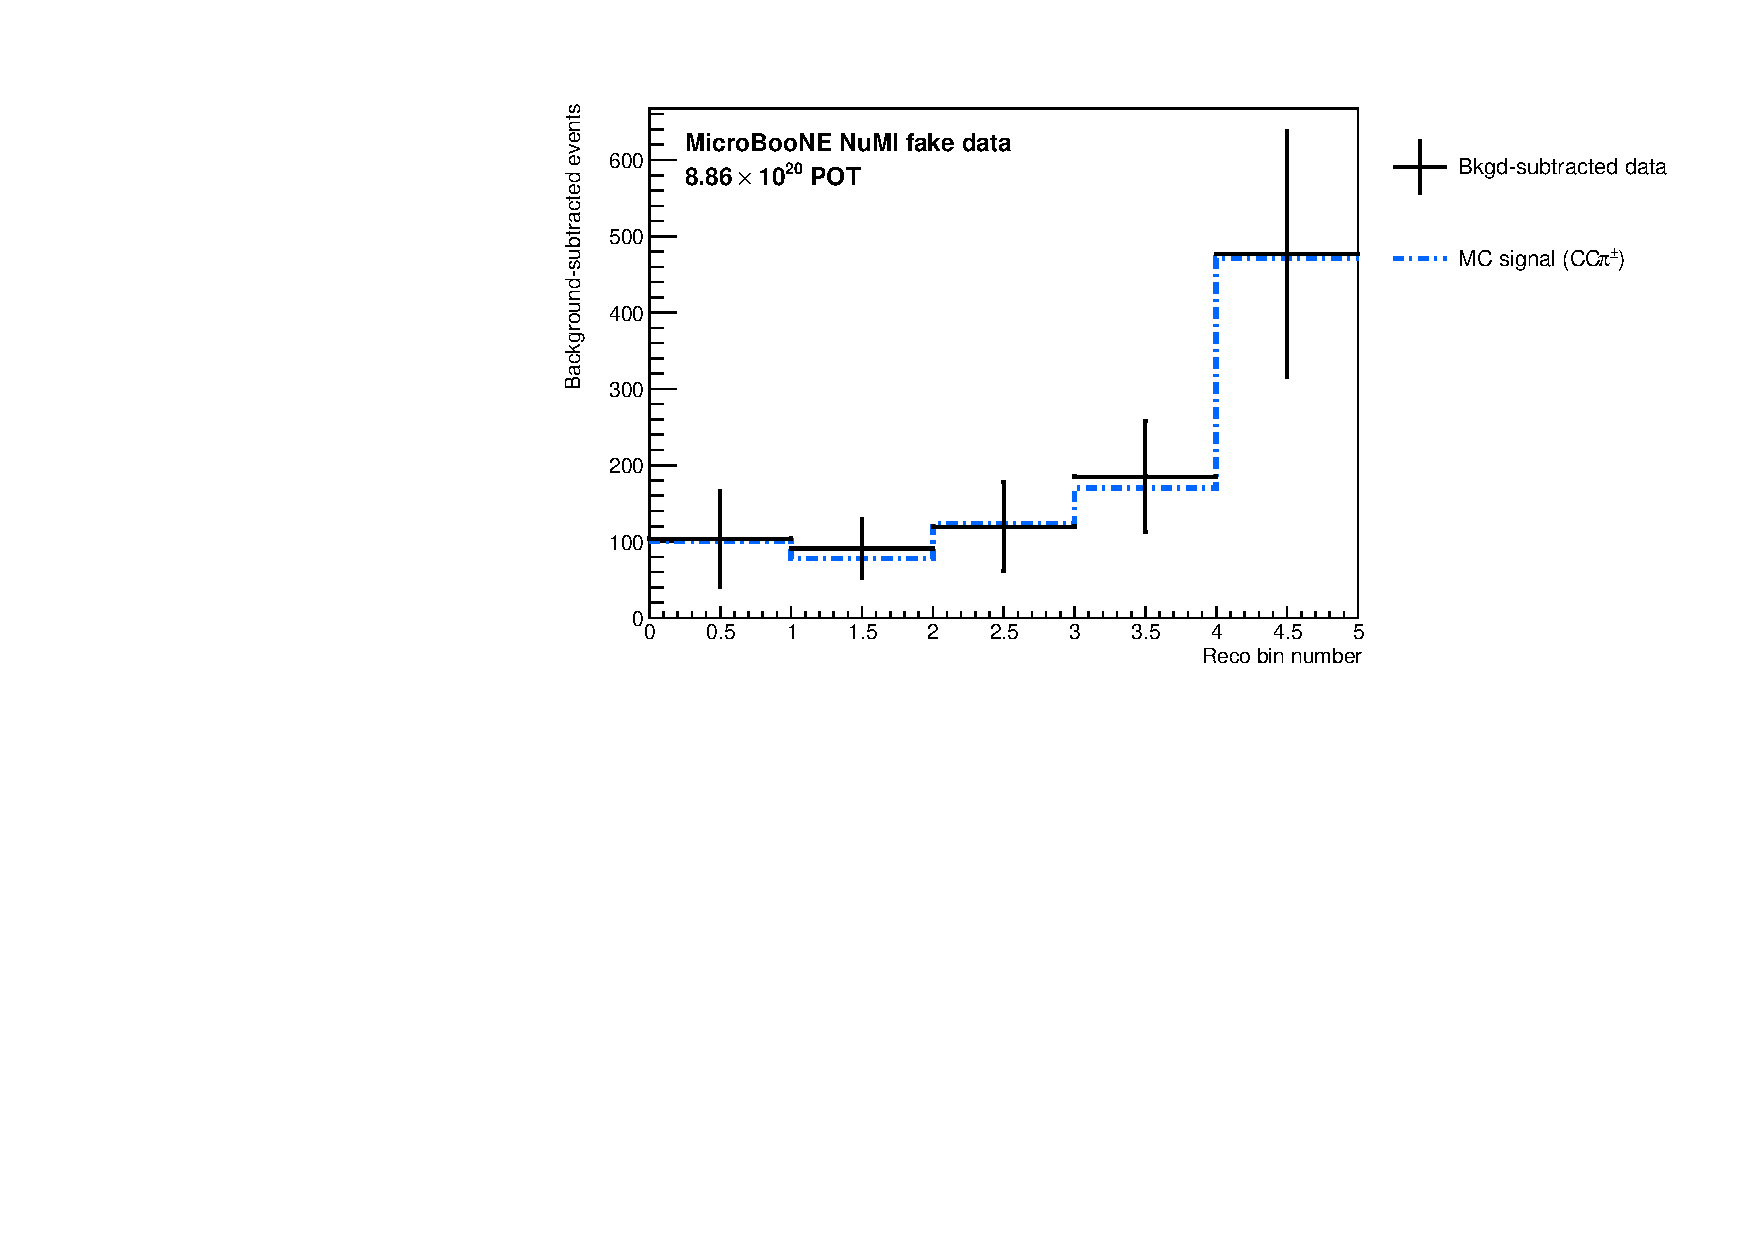
\includegraphics[width=\textwidth]{step2_bsub_costhmu}\caption{$\cos\theta_\mu$}\end{subfigure}

  \vspace{3mm}
  \begin{subfigure}[b]{0.32\textwidth}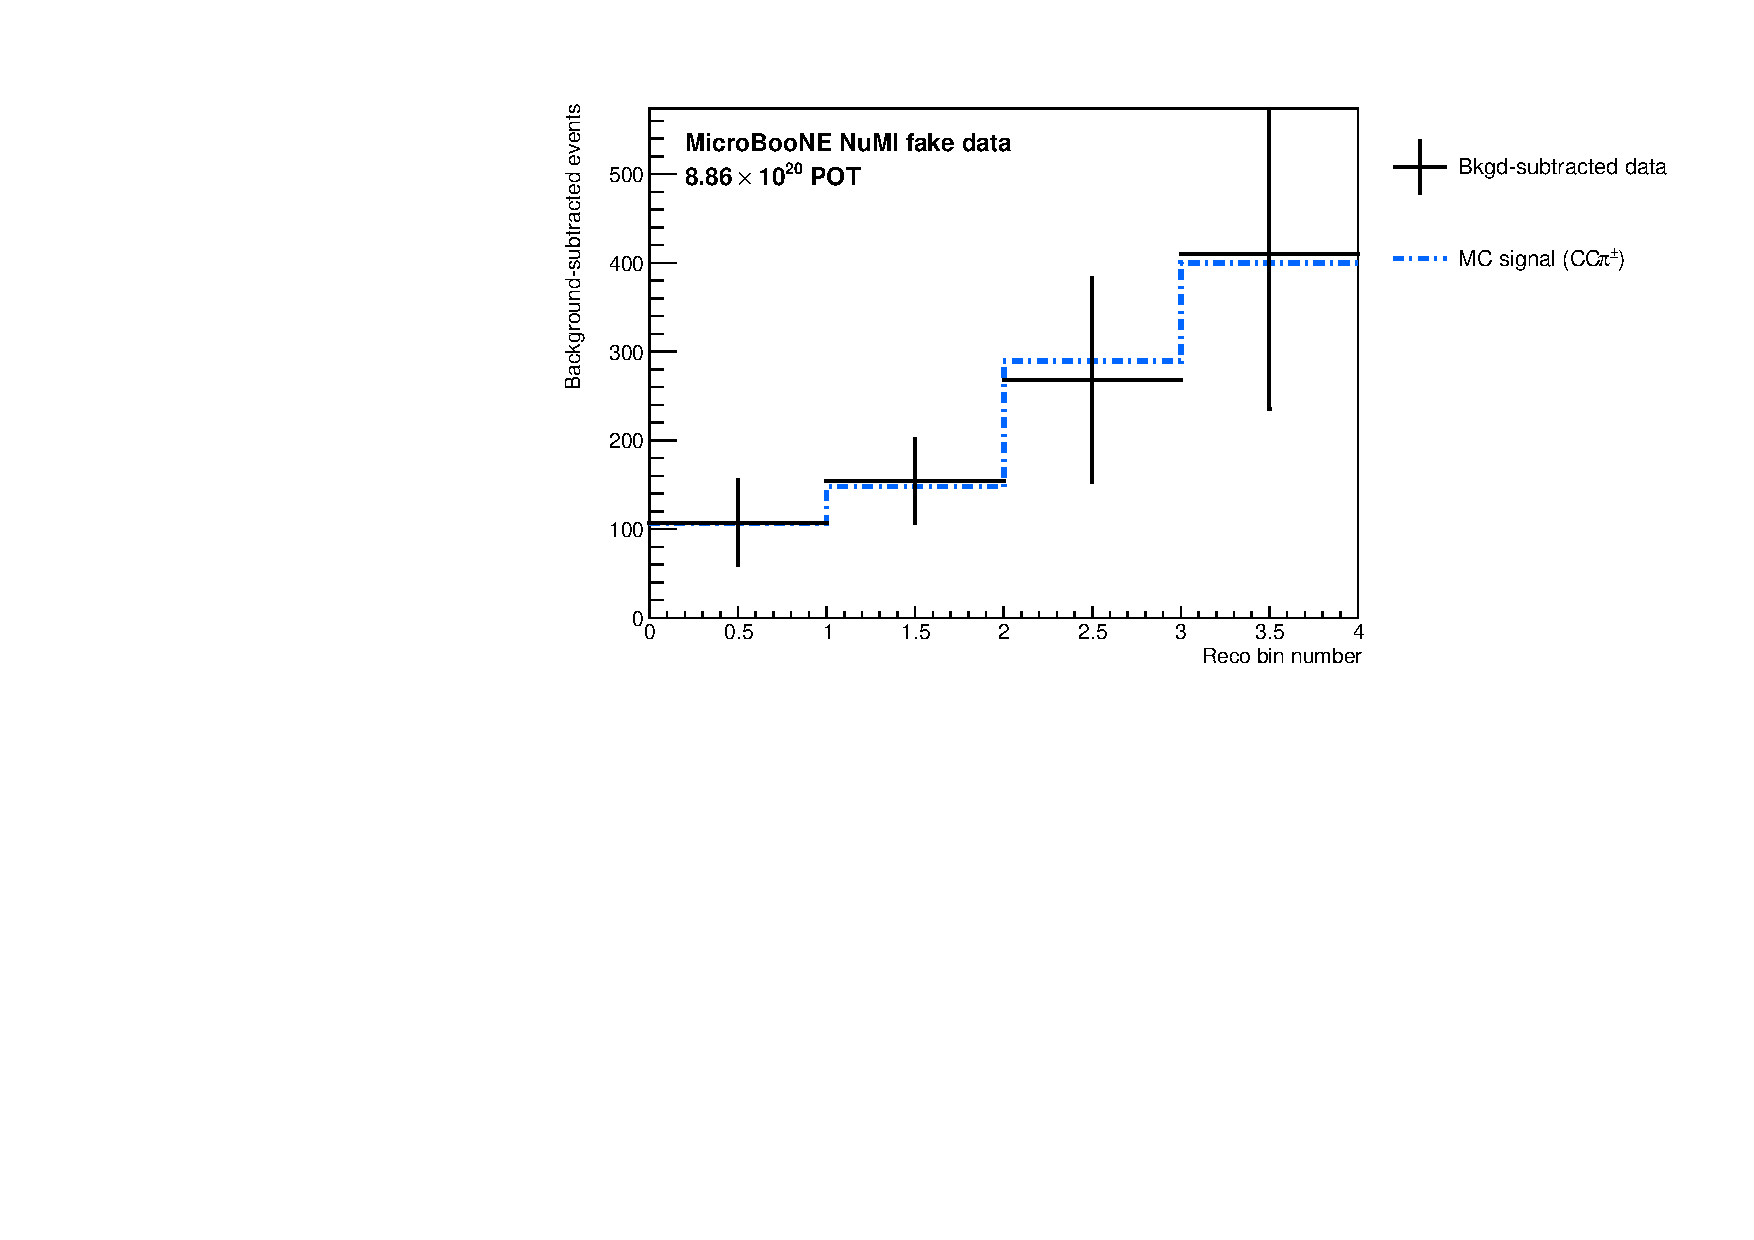
\includegraphics[width=\textwidth]{step2_bsub_costhpi}\caption{$\cos\theta_\pi$}\end{subfigure}\hfill
  \begin{subfigure}[b]{0.32\textwidth}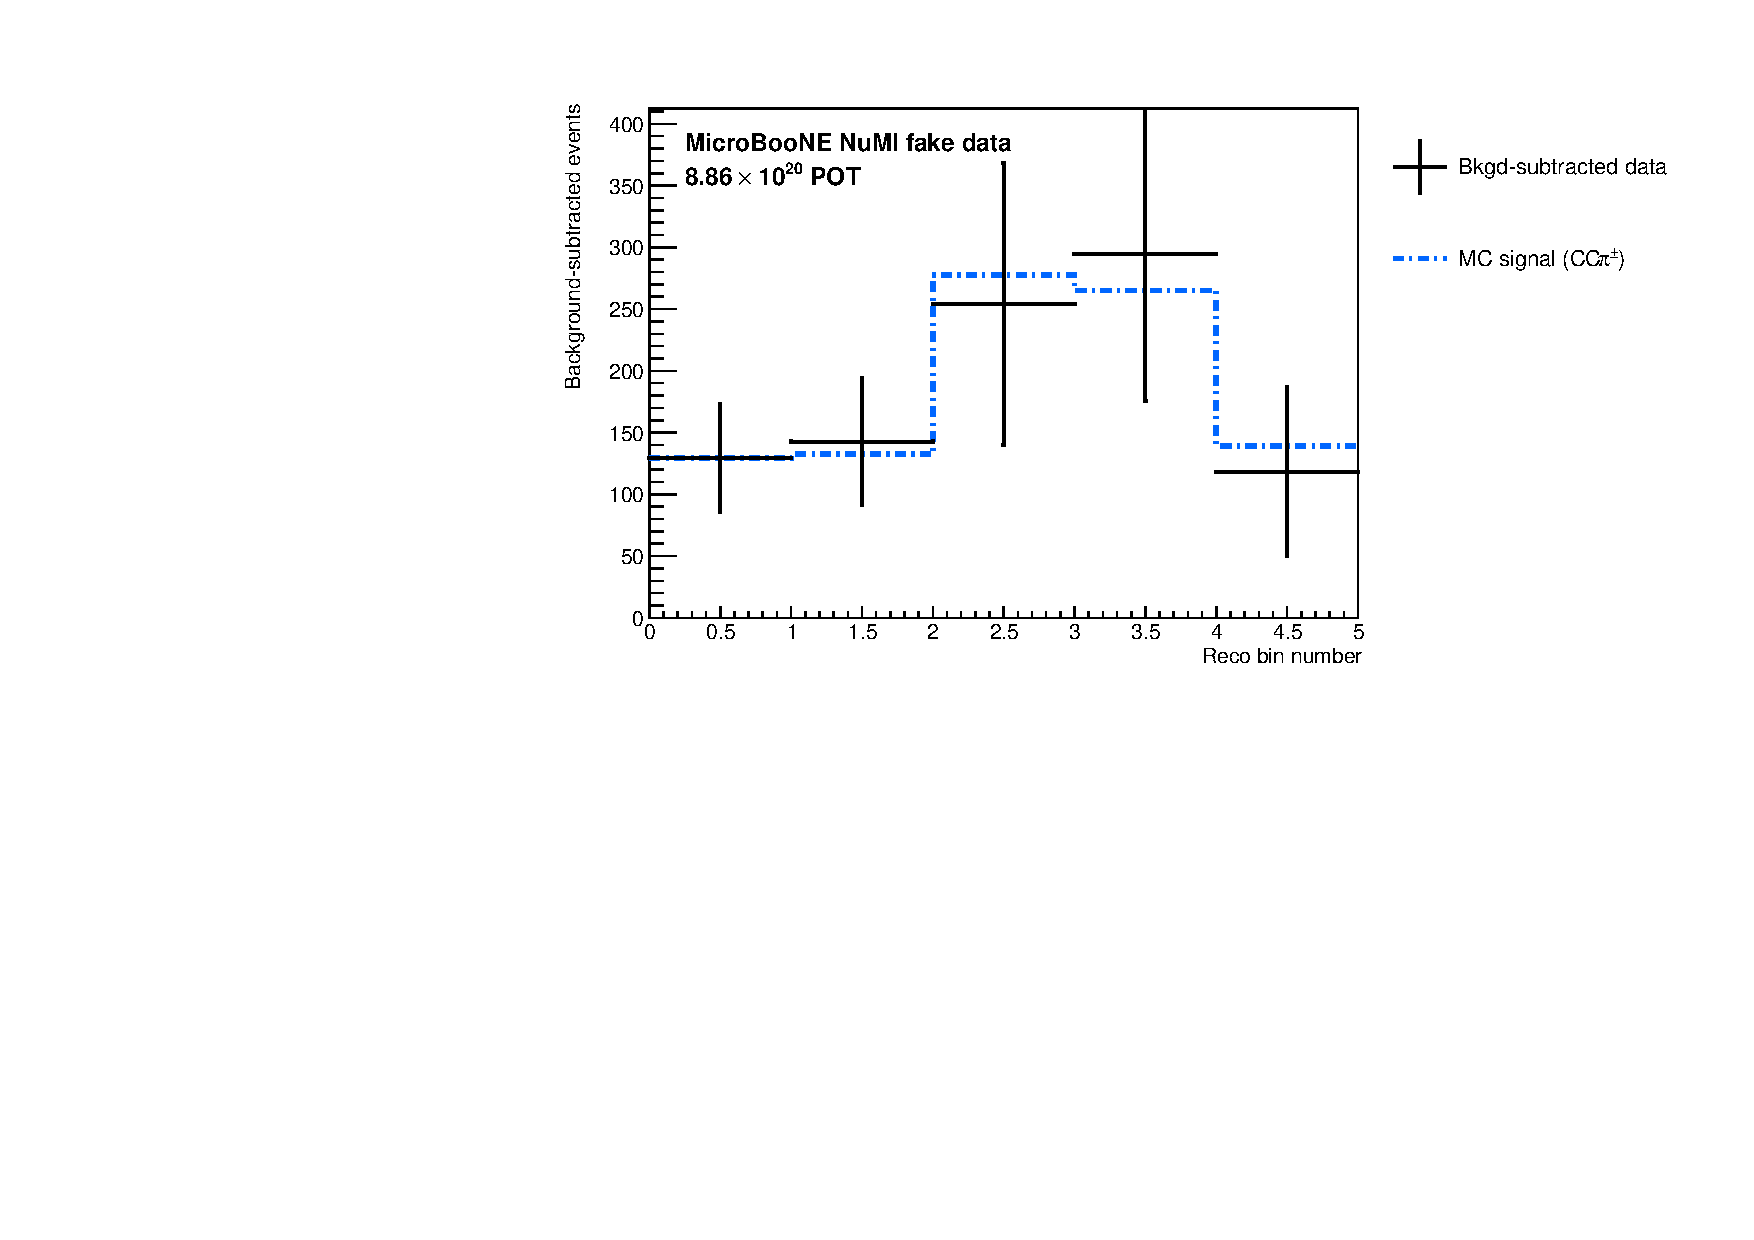
\includegraphics[width=\textwidth]{step2_bsub_thmupi}\caption{$\theta_{\mu\pi}$}\end{subfigure}\hfill
  \begin{subfigure}[b]{0.32\textwidth}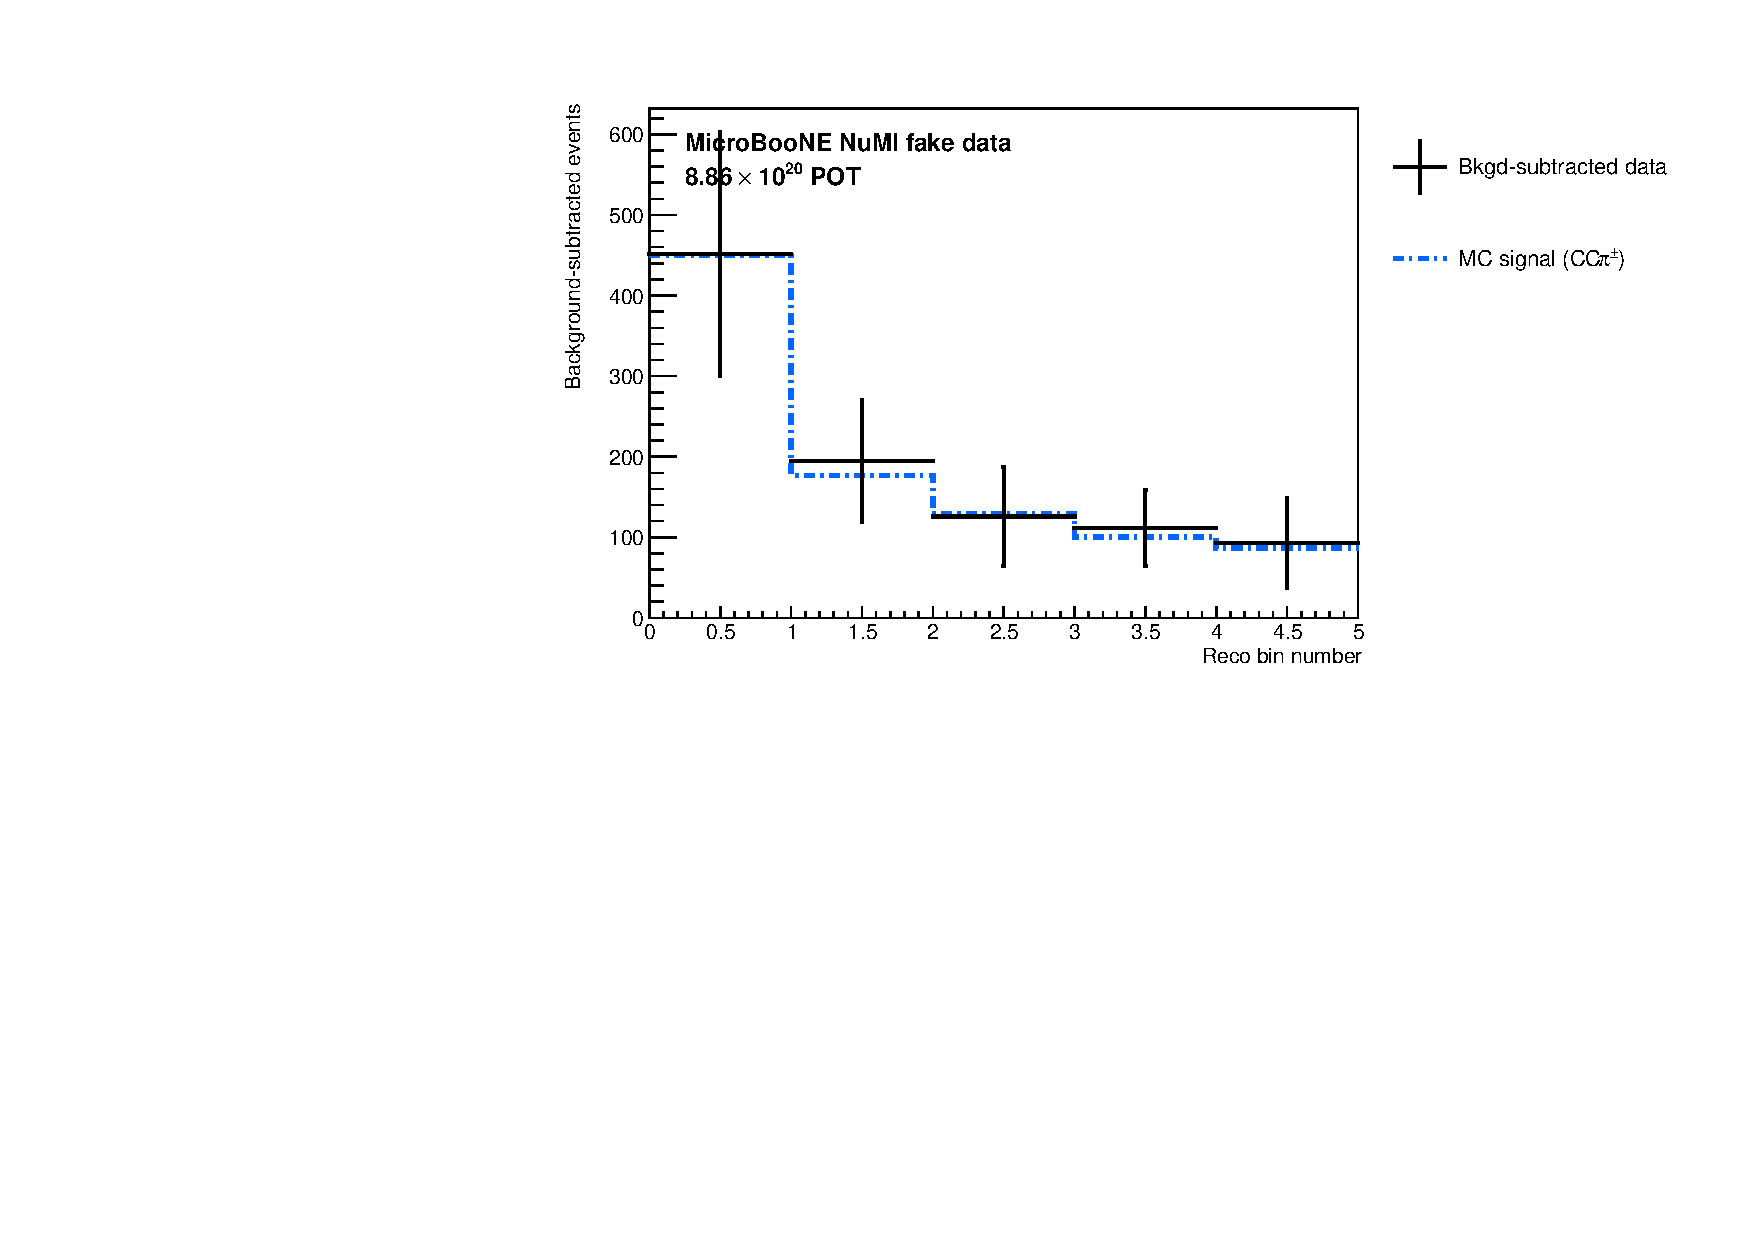
\includegraphics[width=\textwidth]{step2_bsub_thetamu}\caption{$\theta_\mu$}\end{subfigure}
  \caption{Stage 2, FHC: background-subtracted data compared with the central-value MC
    signal; the input to the unfolding. RHC and combined: Figs.~\ref{fig:chain_bsub_rhc}
    (combined: \suppref{Fig.}{fig:chain_bsub_comb}).}
  \label{fig:chain_bsub}
\end{figure}

\begin{figure}[H]
  \centering
  \begin{subfigure}[b]{0.32\textwidth}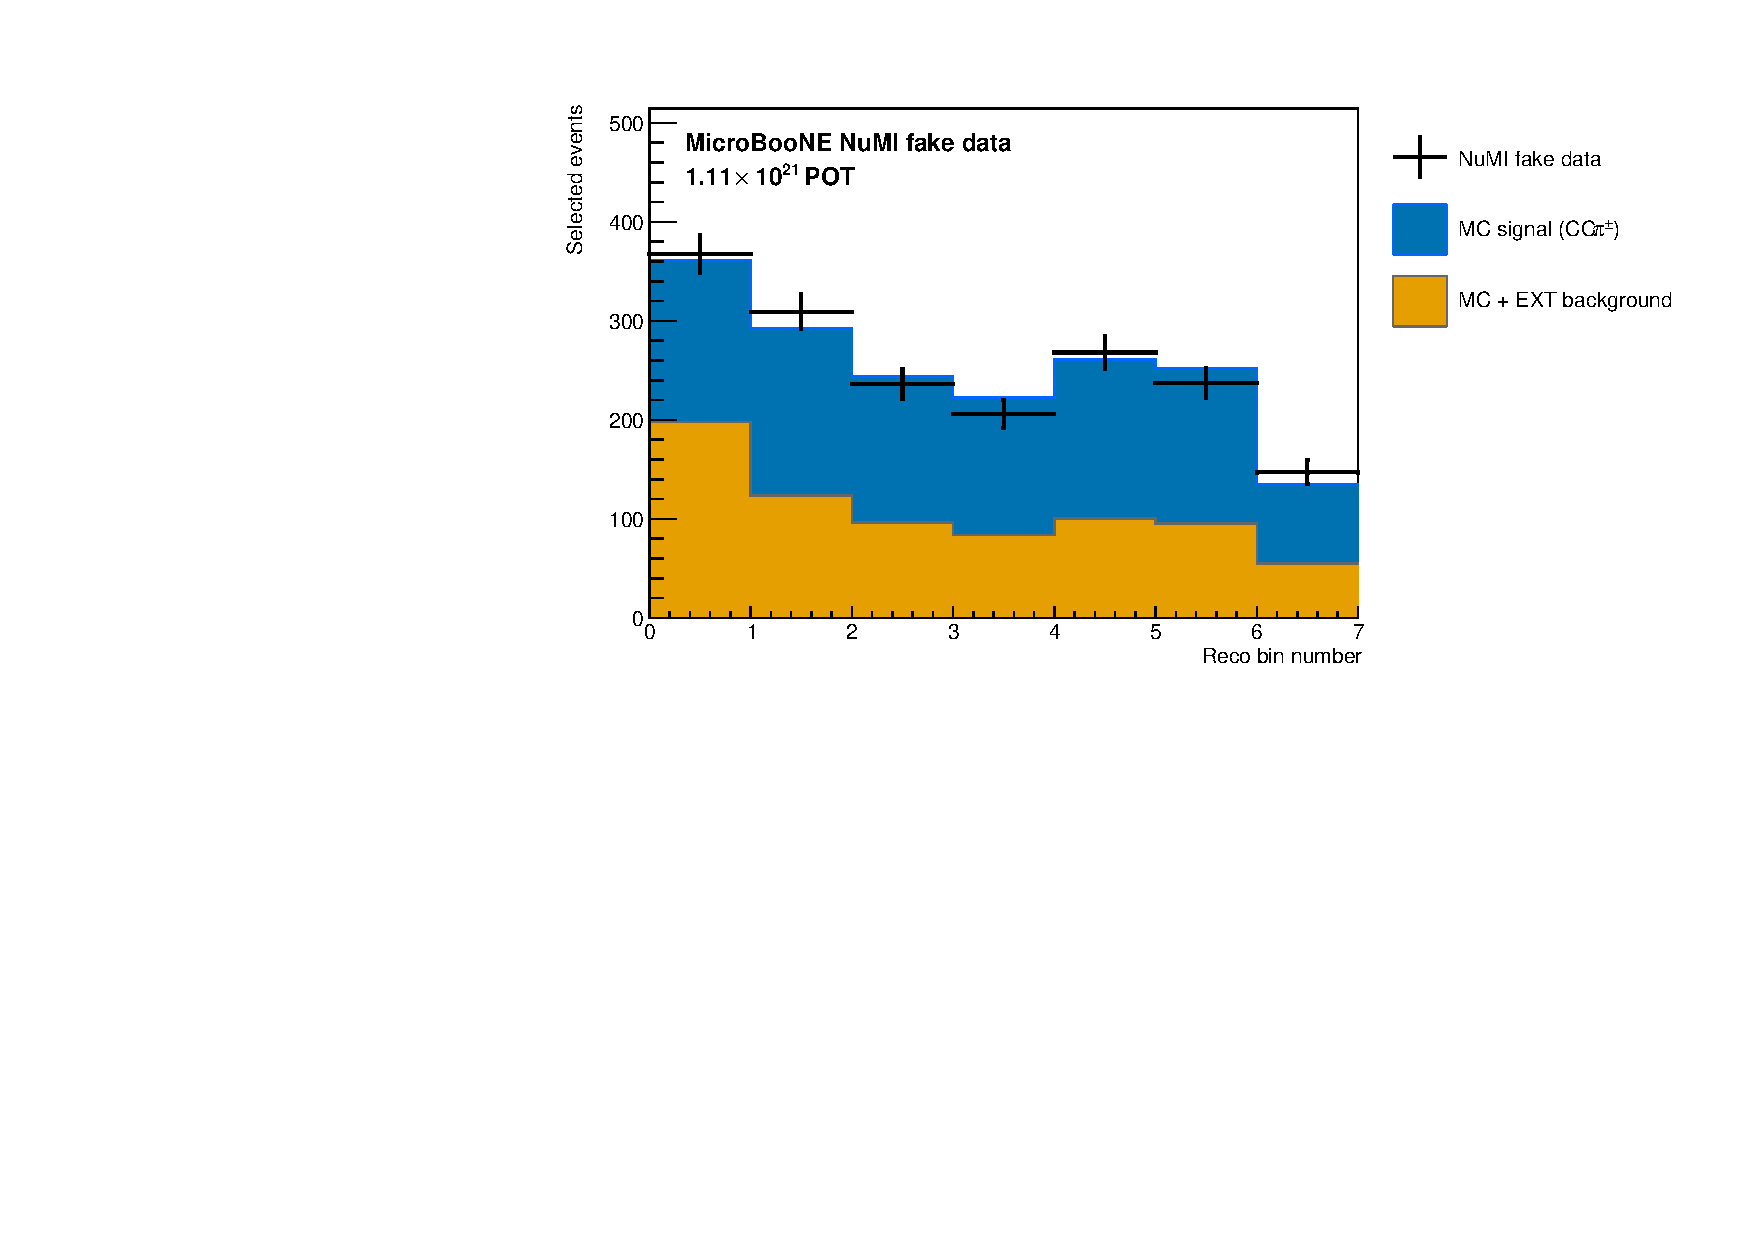
\includegraphics[width=\textwidth]{step1_reco_pmu_RHCFULL}\caption{$p_\mu$}\end{subfigure}\hfill
  \begin{subfigure}[b]{0.32\textwidth}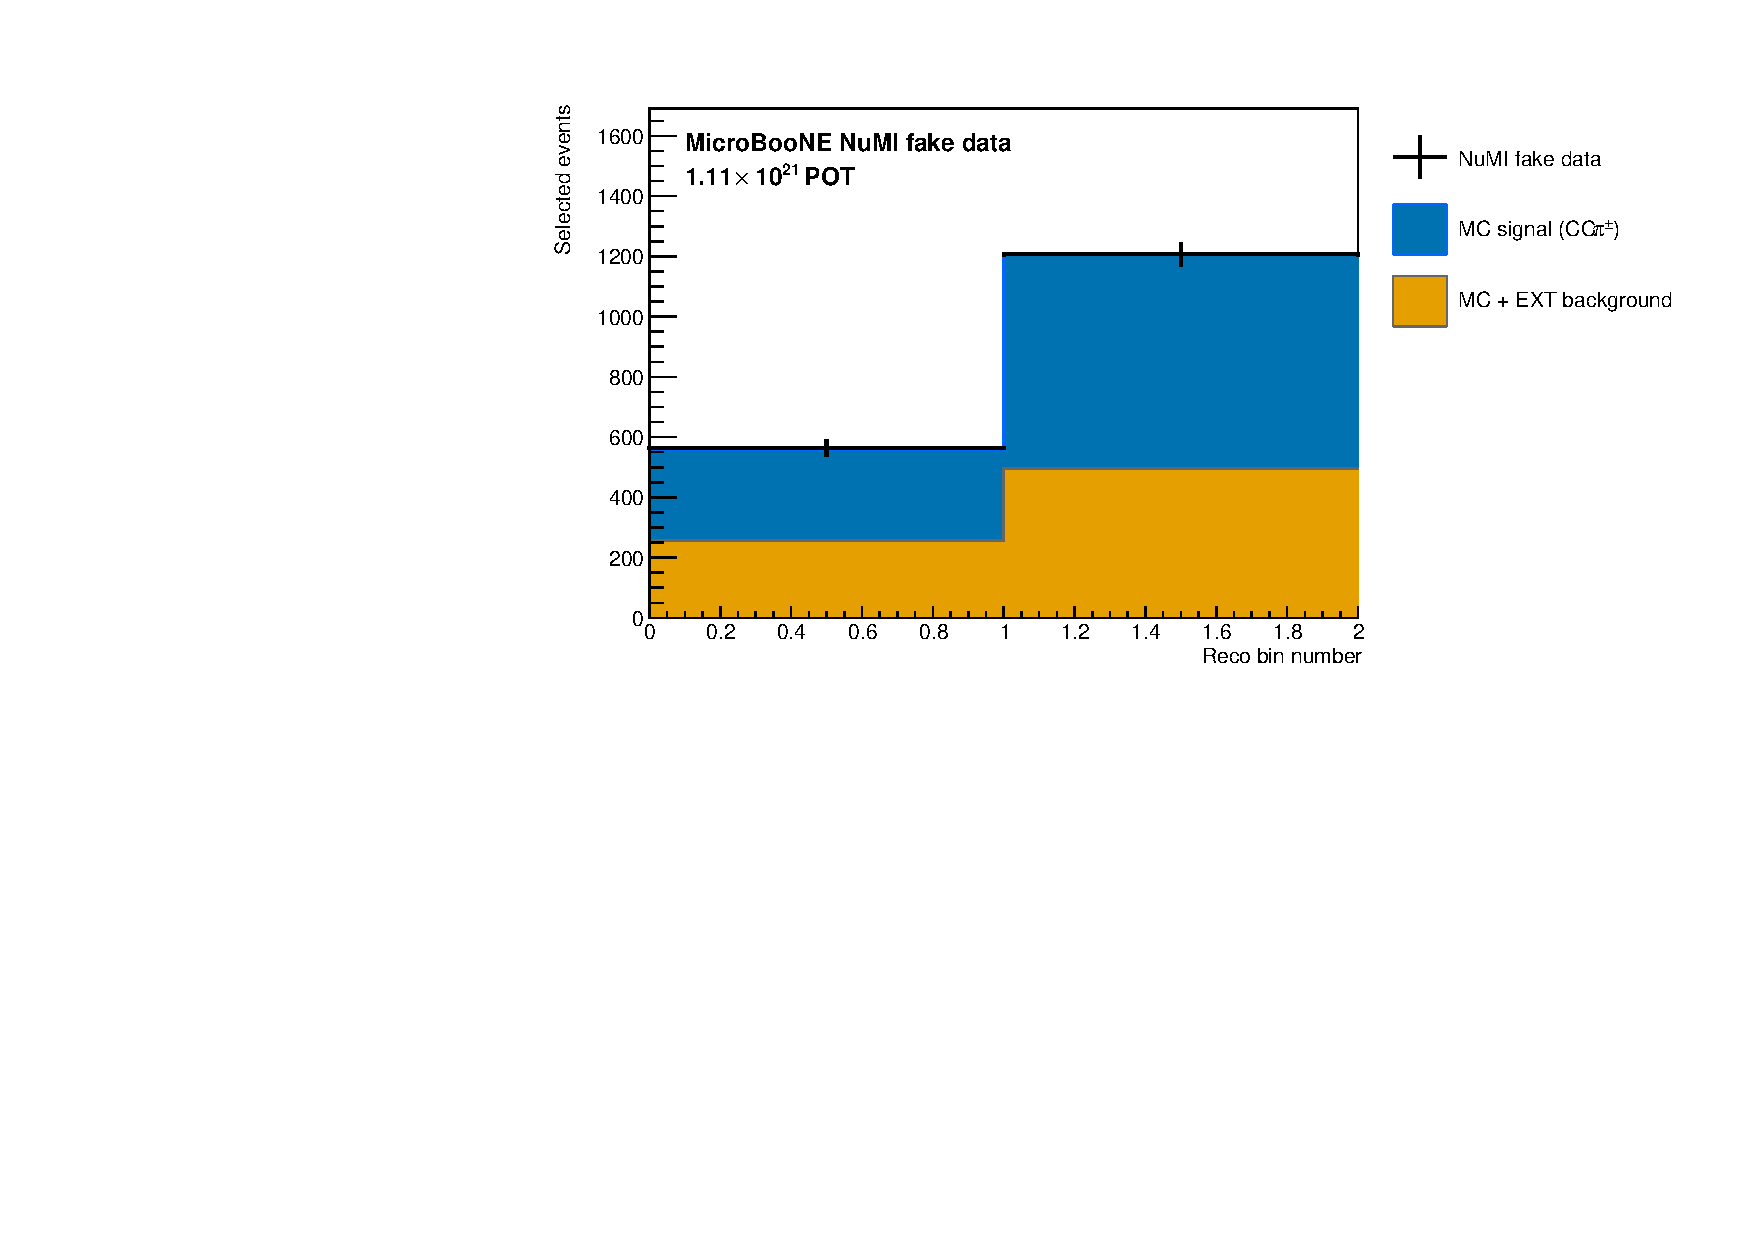
\includegraphics[width=\textwidth]{step1_reco_ppi_RHCFULL}\caption{$p_\pi$}\end{subfigure}\hfill
  \begin{subfigure}[b]{0.32\textwidth}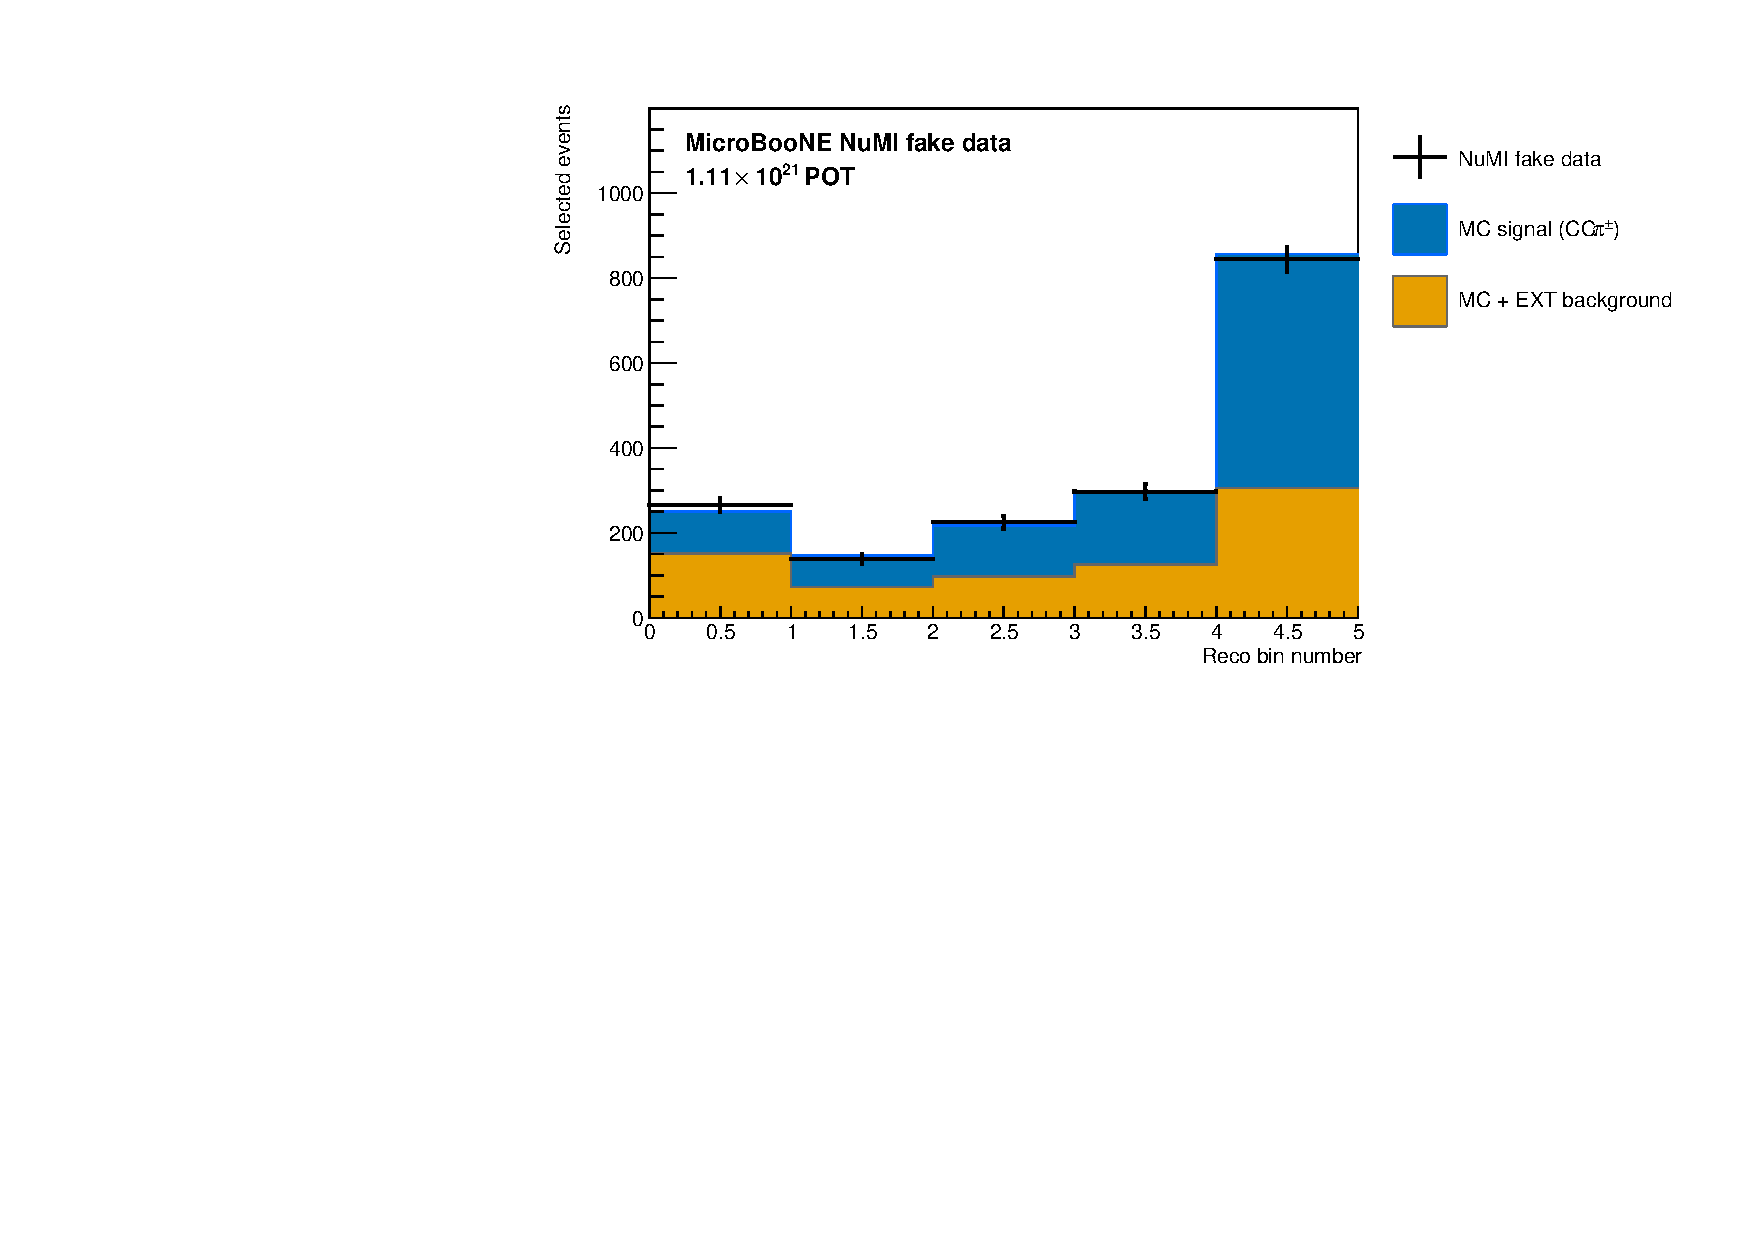
\includegraphics[width=\textwidth]{step1_reco_costhmu_RHCFULL}\caption{$\cos\theta_\mu$}\end{subfigure}

  \vspace{3mm}
  \begin{subfigure}[b]{0.32\textwidth}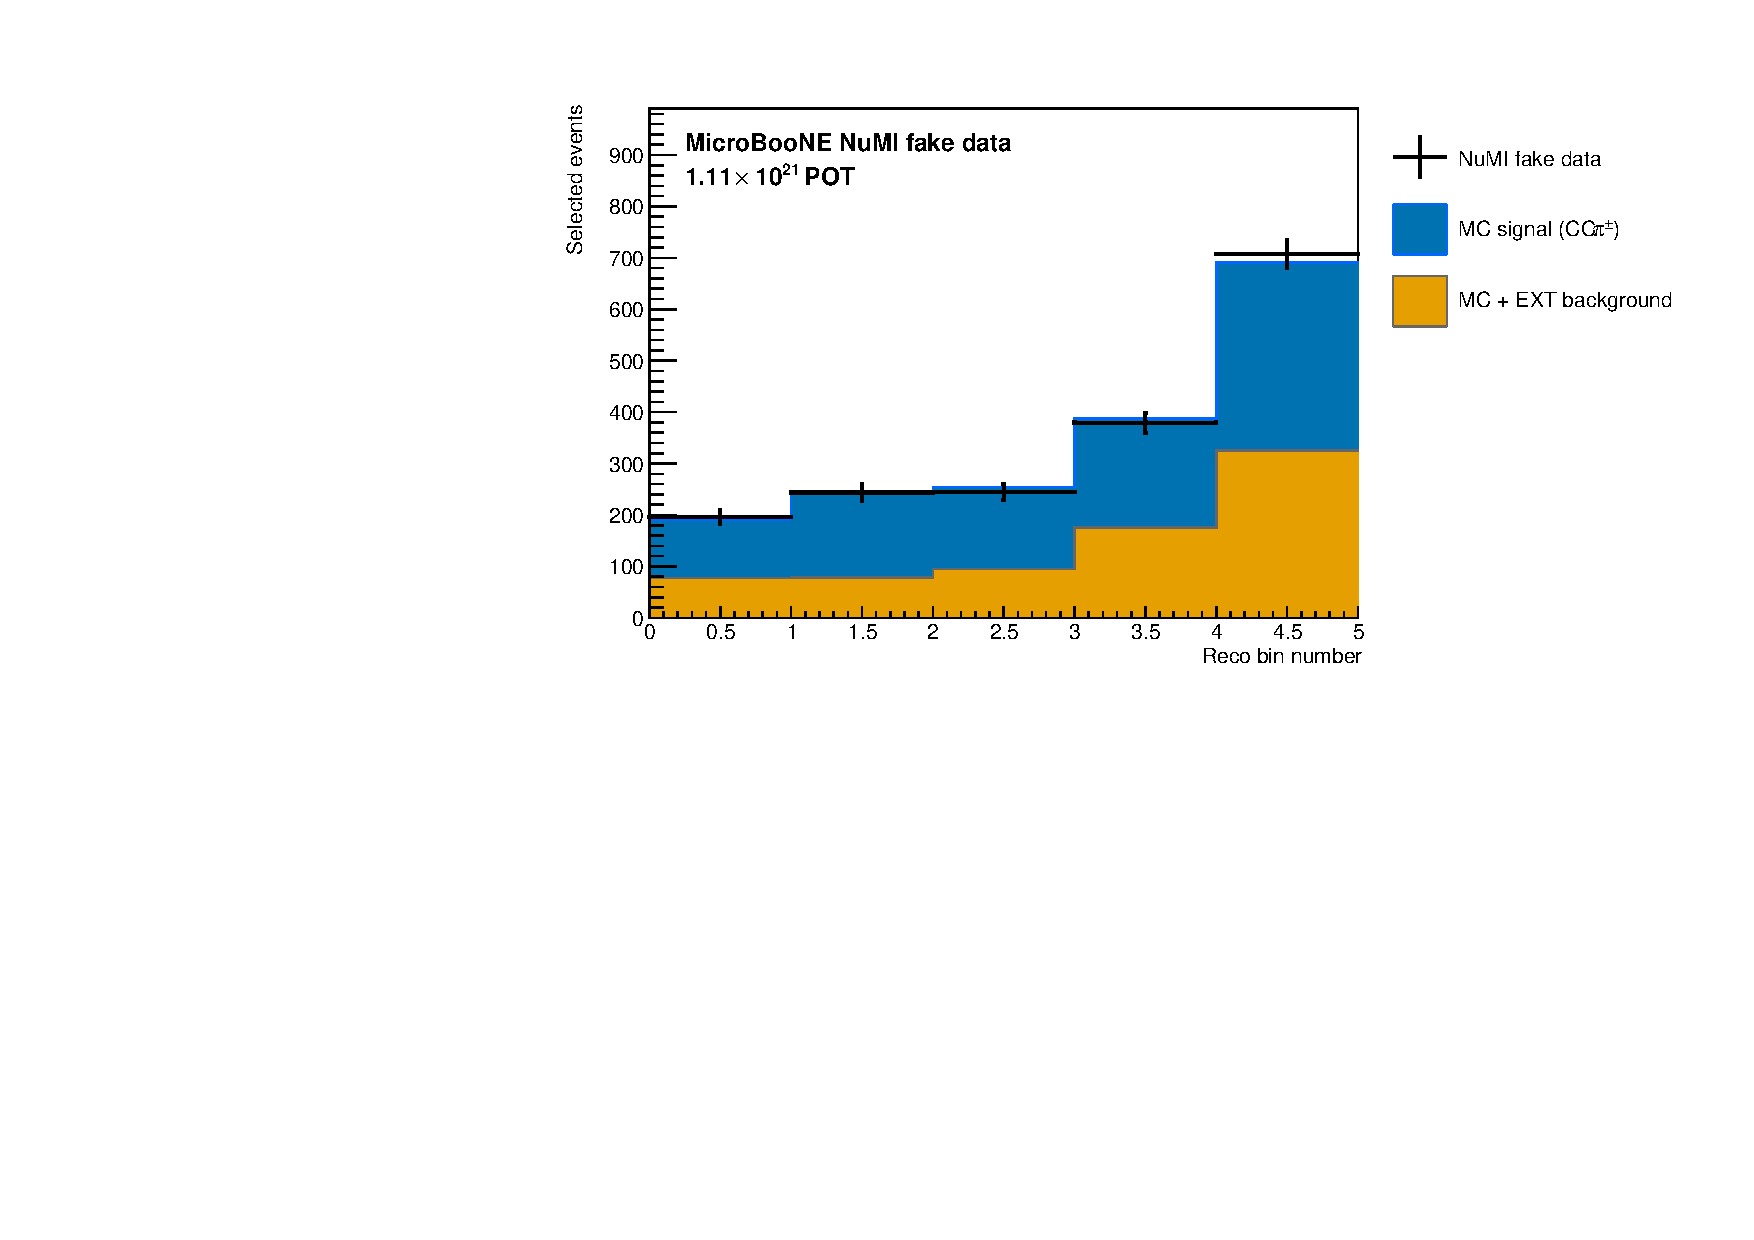
\includegraphics[width=\textwidth]{step1_reco_costhpi_RHCFULL}\caption{$\cos\theta_\pi$}\end{subfigure}\hfill
  \begin{subfigure}[b]{0.32\textwidth}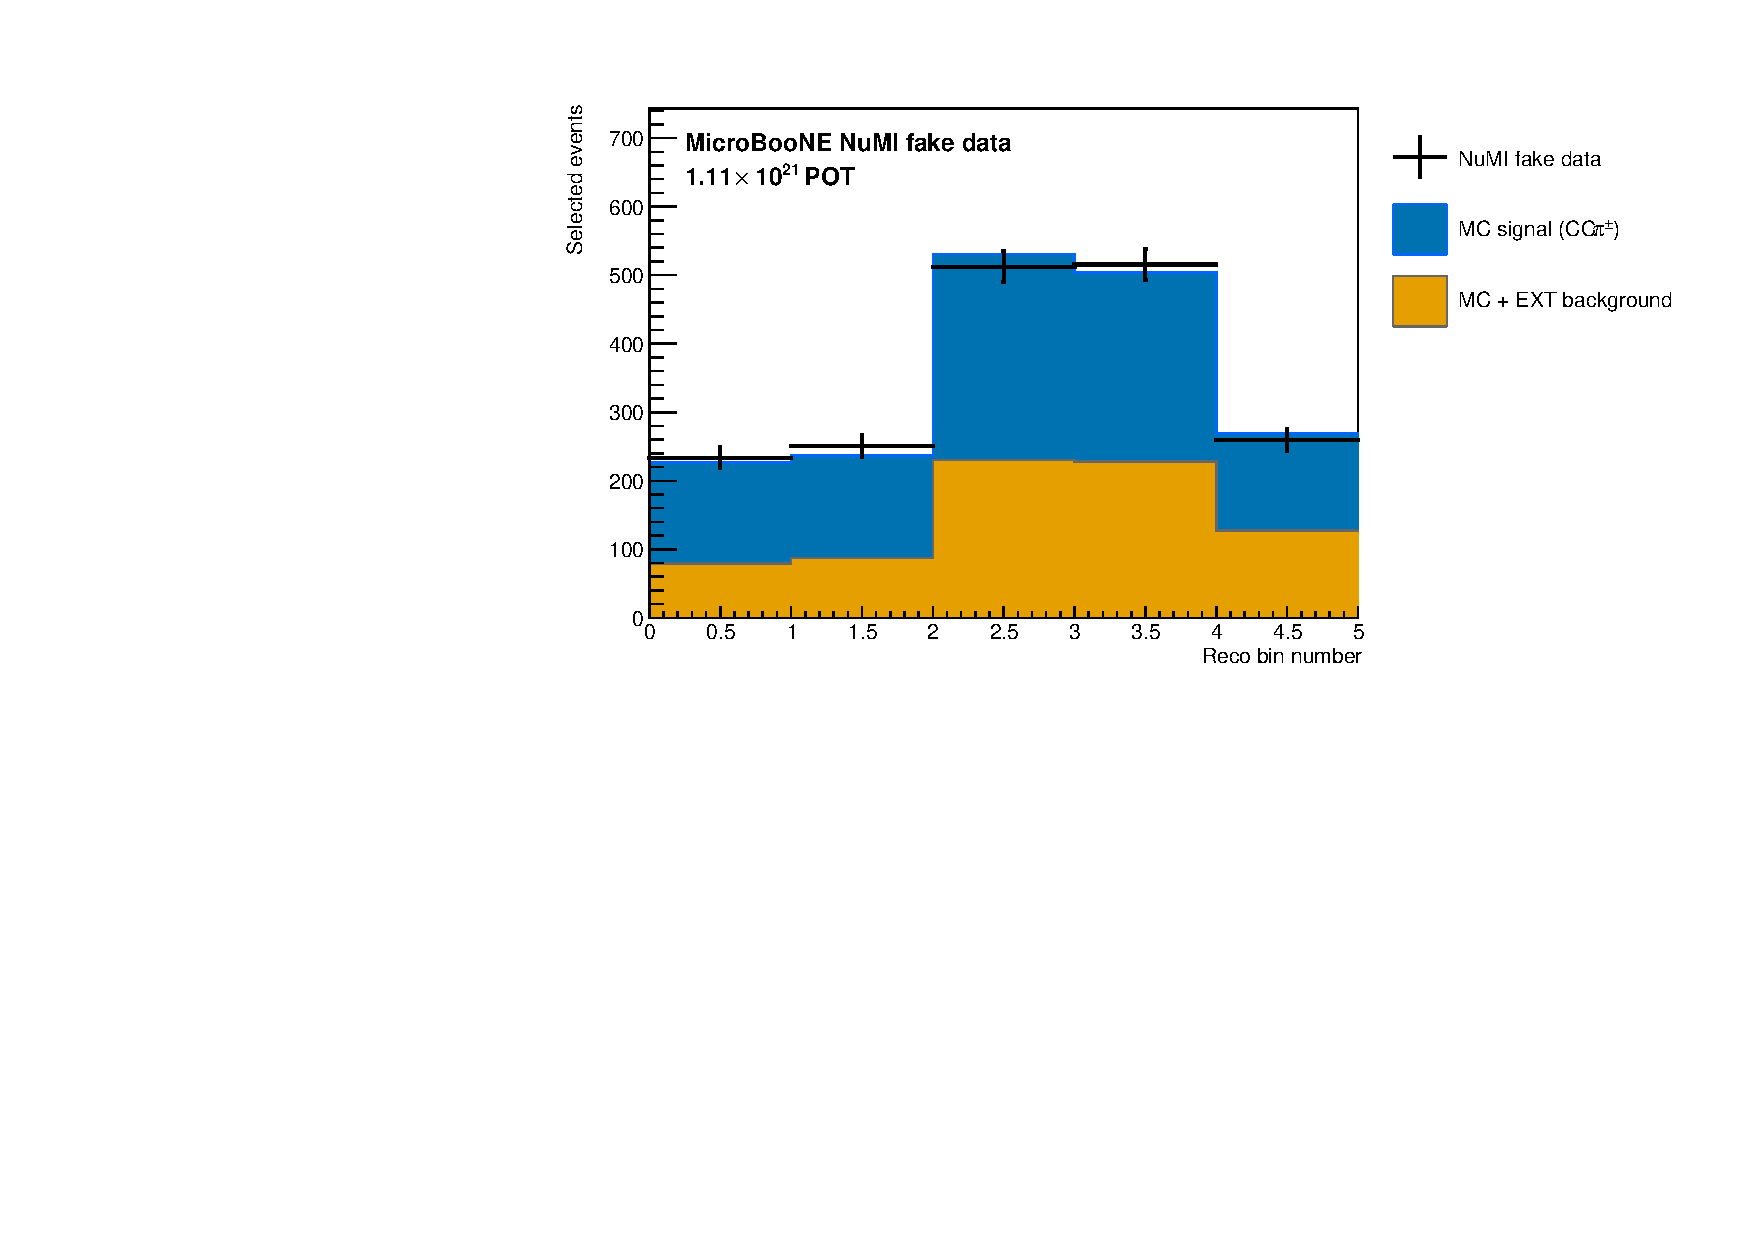
\includegraphics[width=\textwidth]{step1_reco_thmupi_RHCFULL}\caption{$\theta_{\mu\pi}$}\end{subfigure}\hfill
  \begin{subfigure}[b]{0.32\textwidth}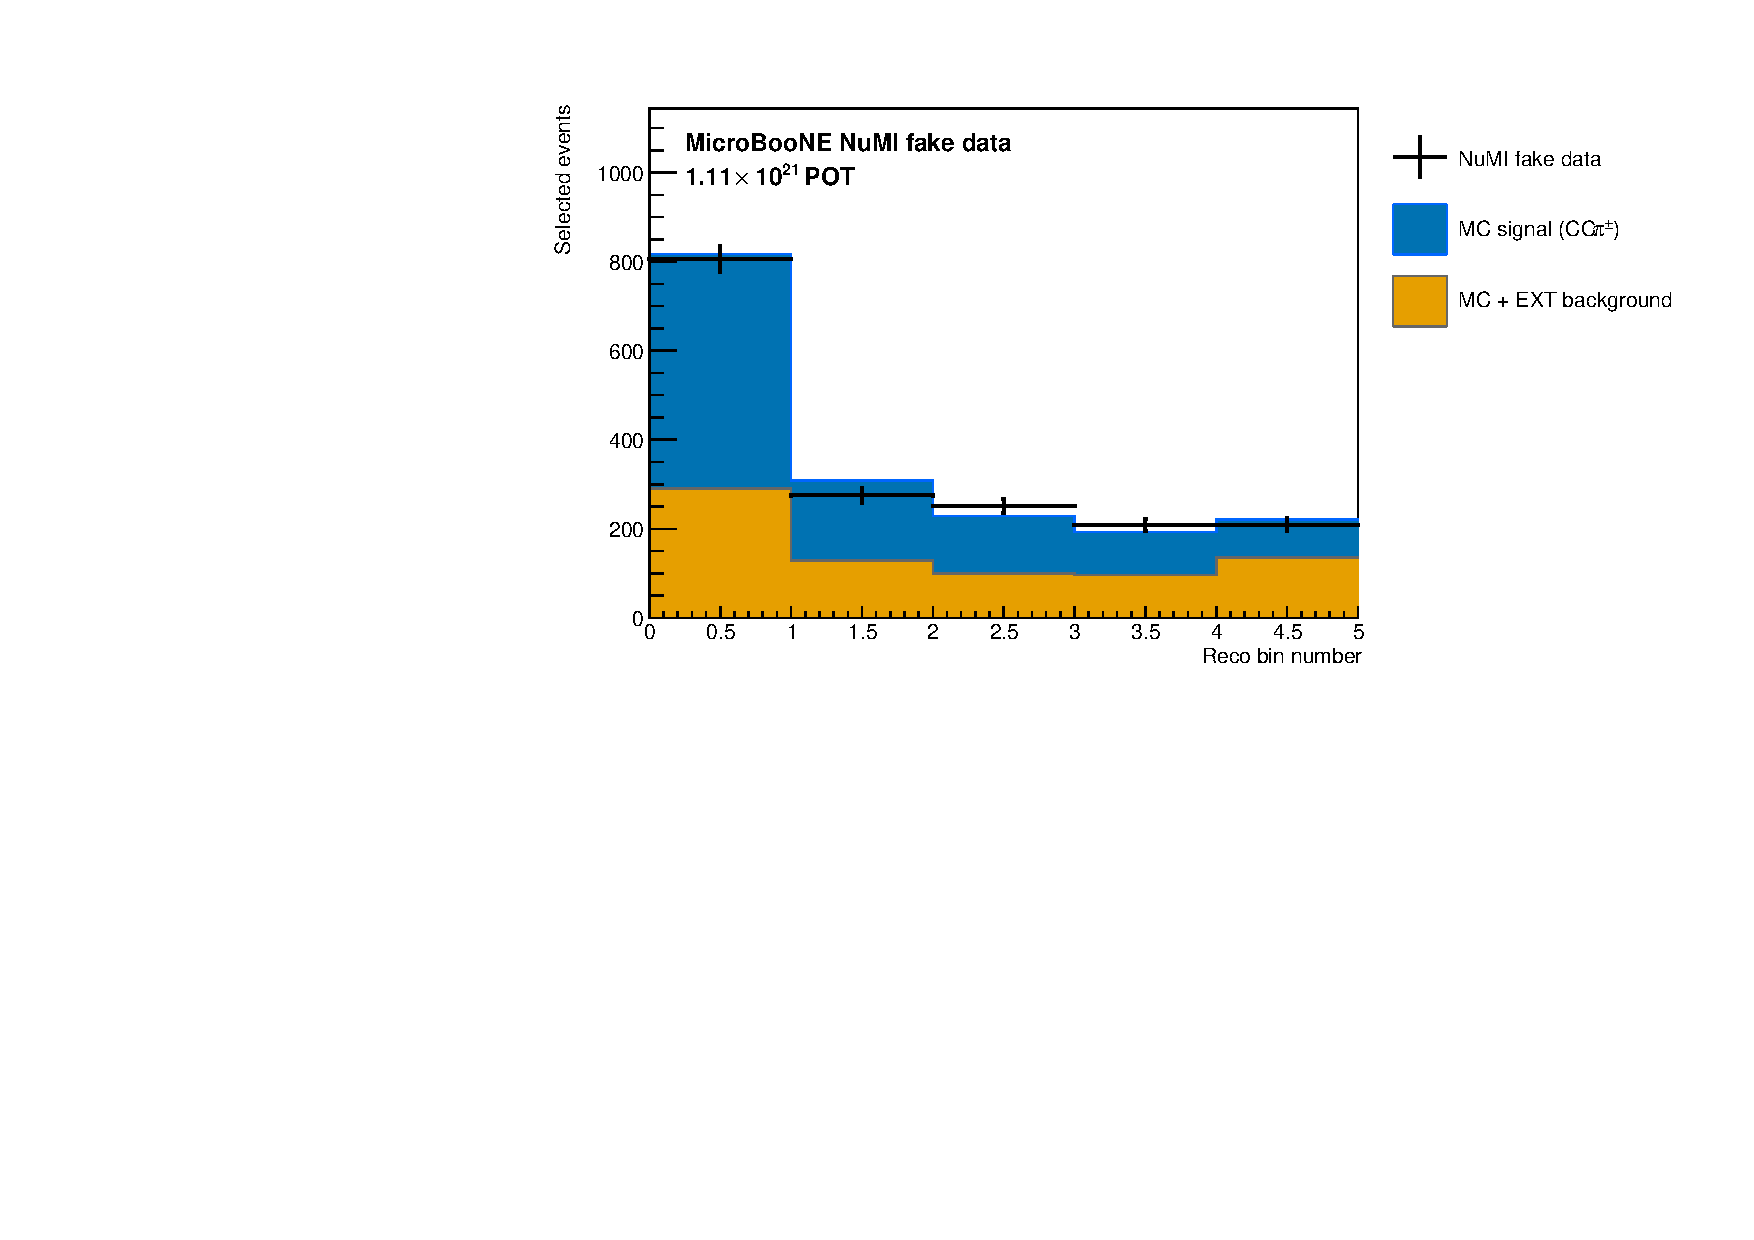
\includegraphics[width=\textwidth]{step1_reco_thetamu_RHCFULL}\caption{$\theta_\mu$}\end{subfigure}
  \caption{Stage 1, RHC: selected reconstructed spectra scaled to the full RHC exposure, MC split into signal and background.}
  \label{fig:chain_reco_rhc}
\end{figure}

\begin{figure}[H]
  \centering
  \begin{subfigure}[b]{0.32\textwidth}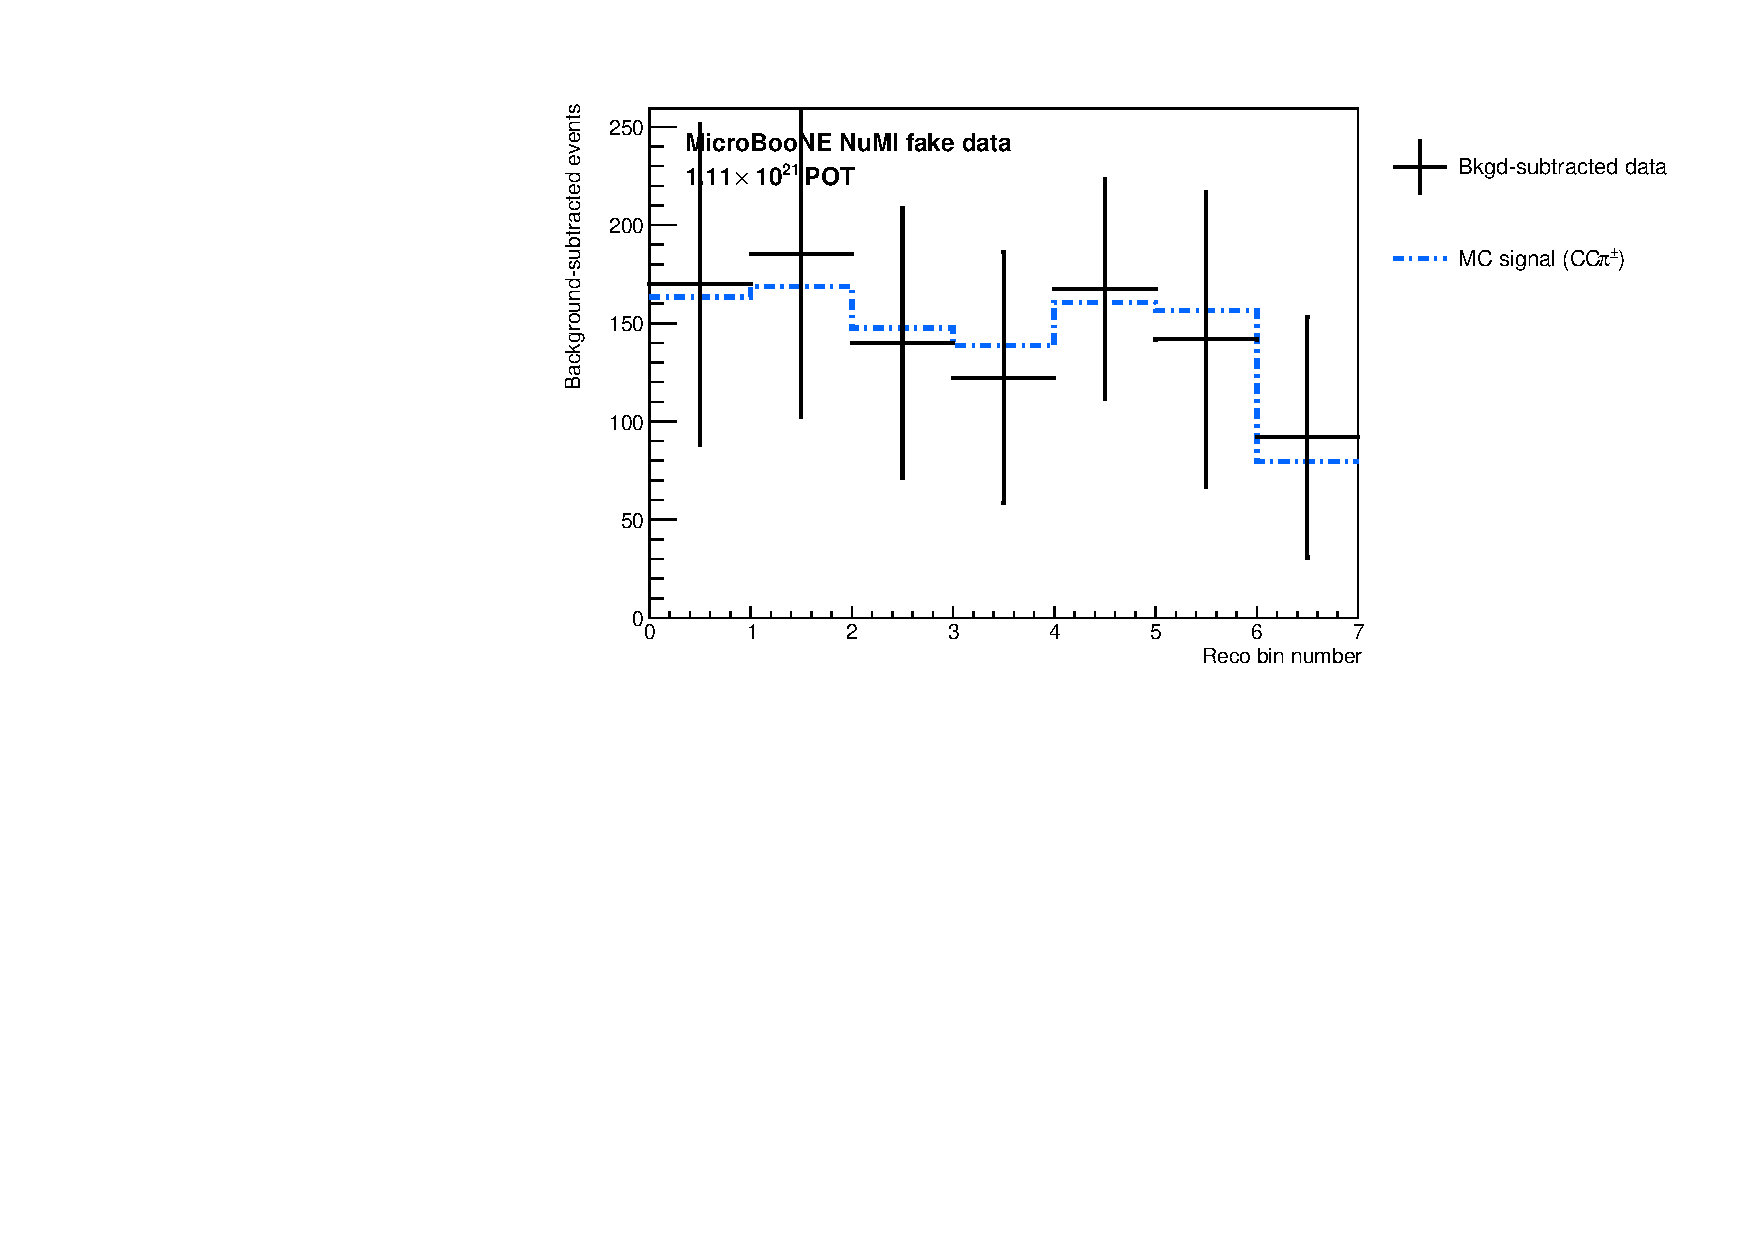
\includegraphics[width=\textwidth]{step2_bsub_pmu_RHCFULL}\caption{$p_\mu$}\end{subfigure}\hfill
  \begin{subfigure}[b]{0.32\textwidth}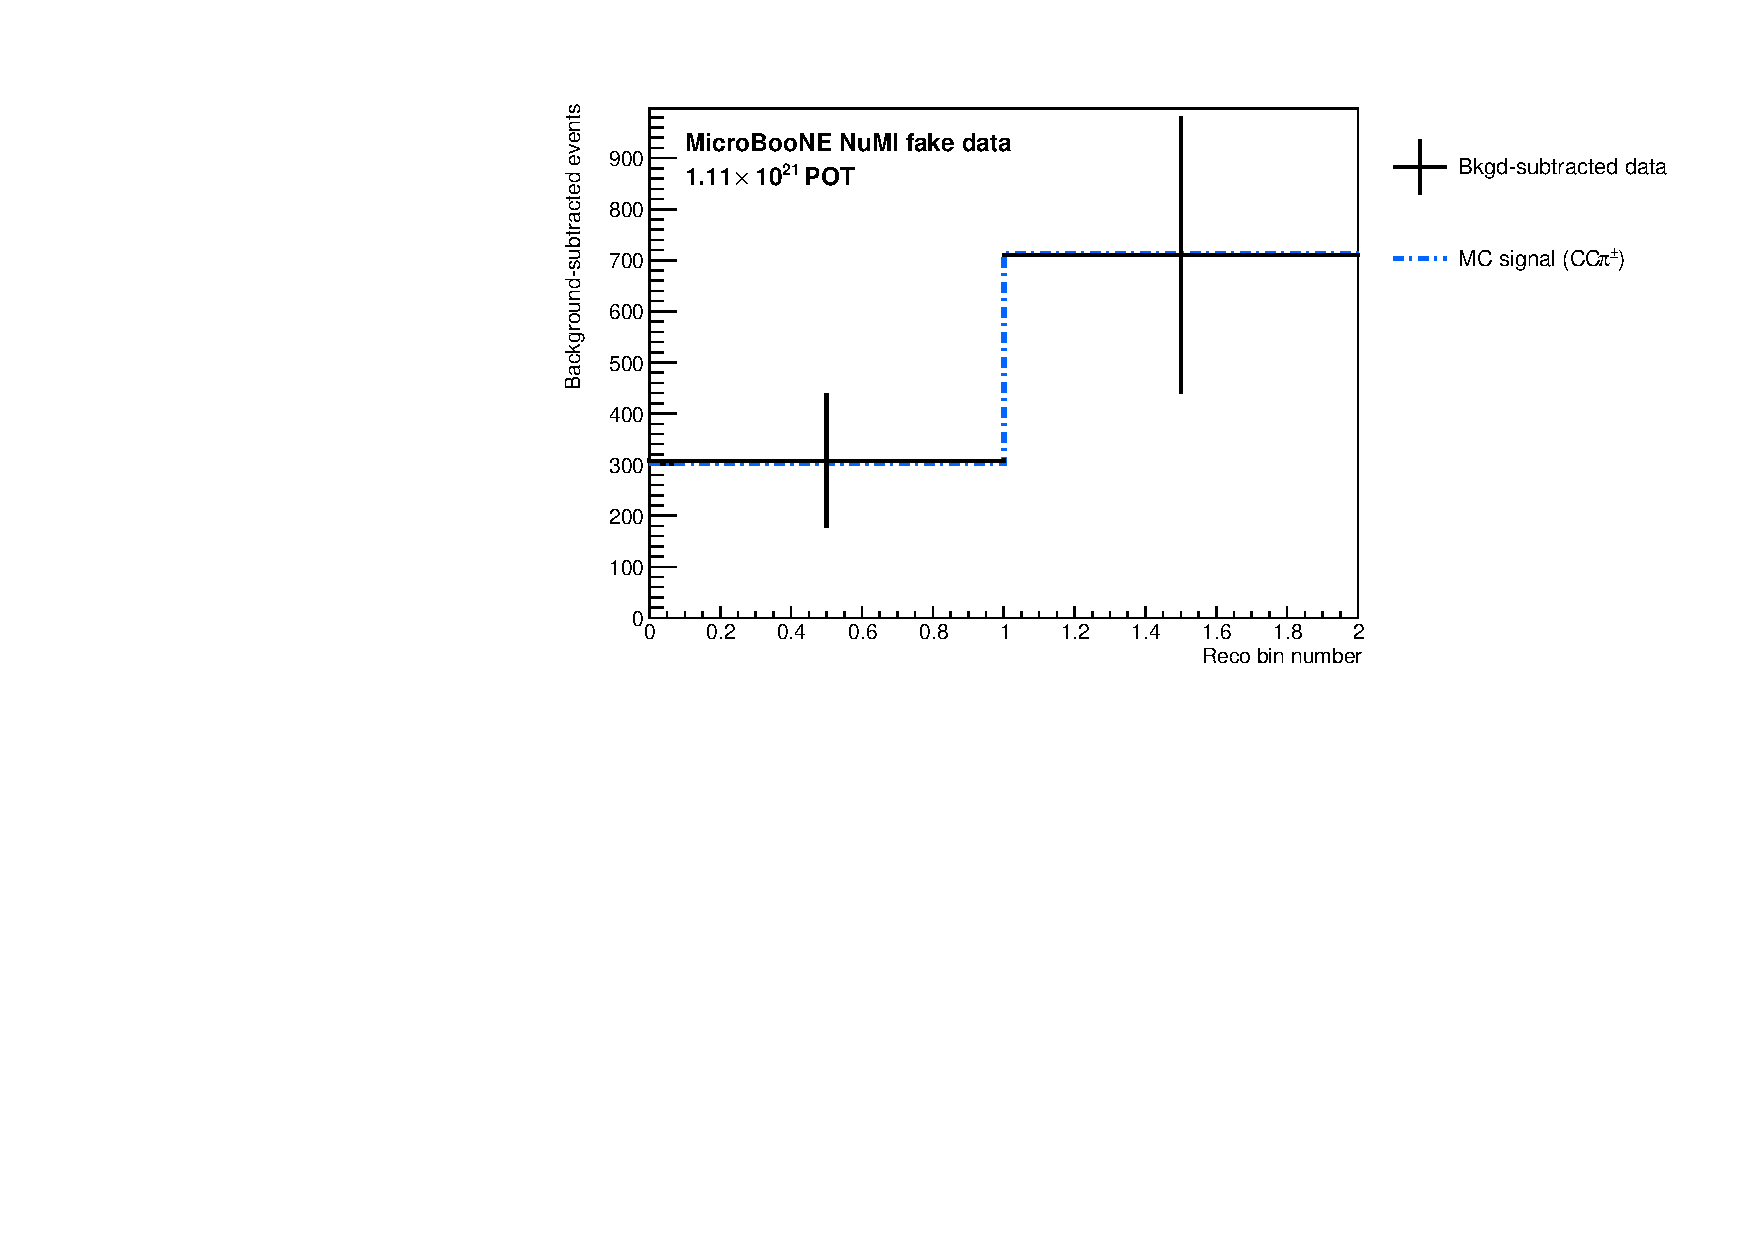
\includegraphics[width=\textwidth]{step2_bsub_ppi_RHCFULL}\caption{$p_\pi$}\end{subfigure}\hfill
  \begin{subfigure}[b]{0.32\textwidth}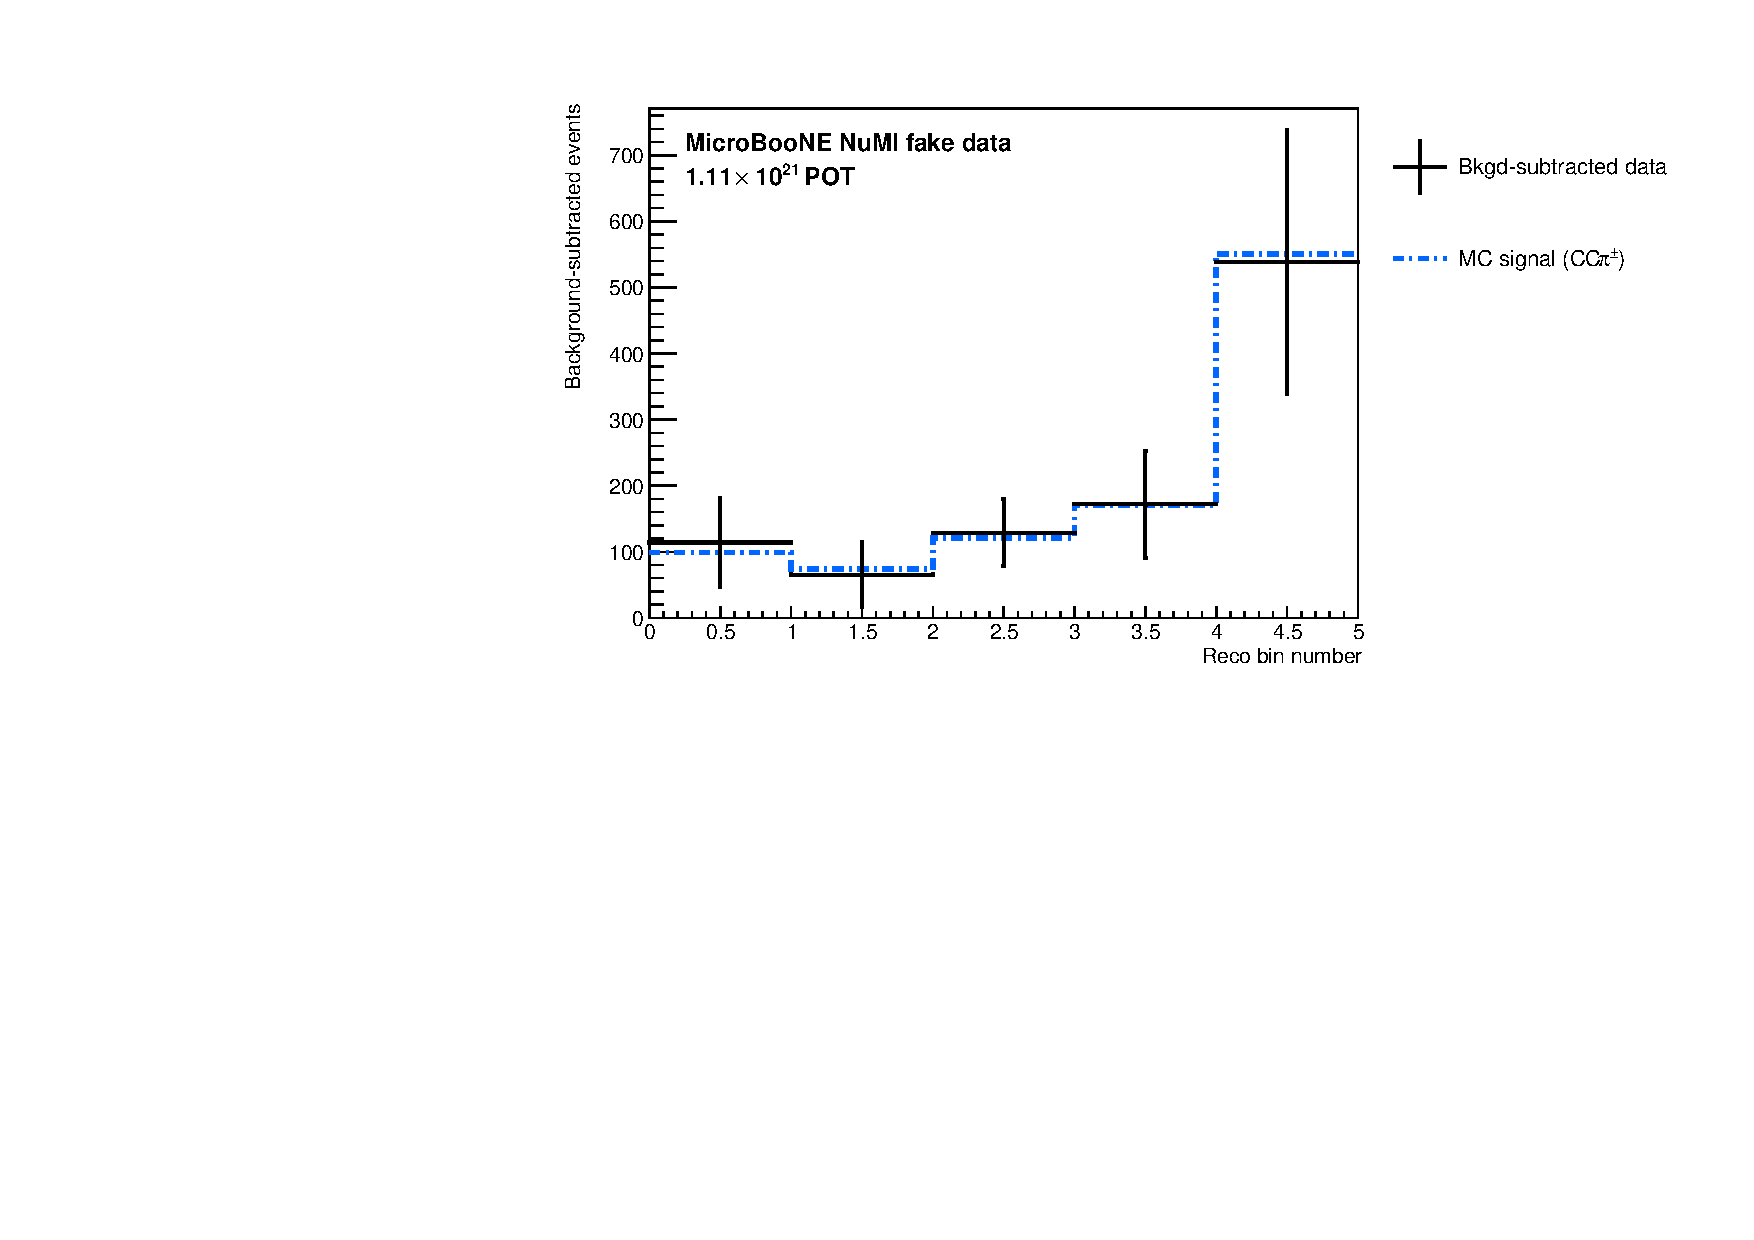
\includegraphics[width=\textwidth]{step2_bsub_costhmu_RHCFULL}\caption{$\cos\theta_\mu$}\end{subfigure}

  \vspace{3mm}
  \begin{subfigure}[b]{0.32\textwidth}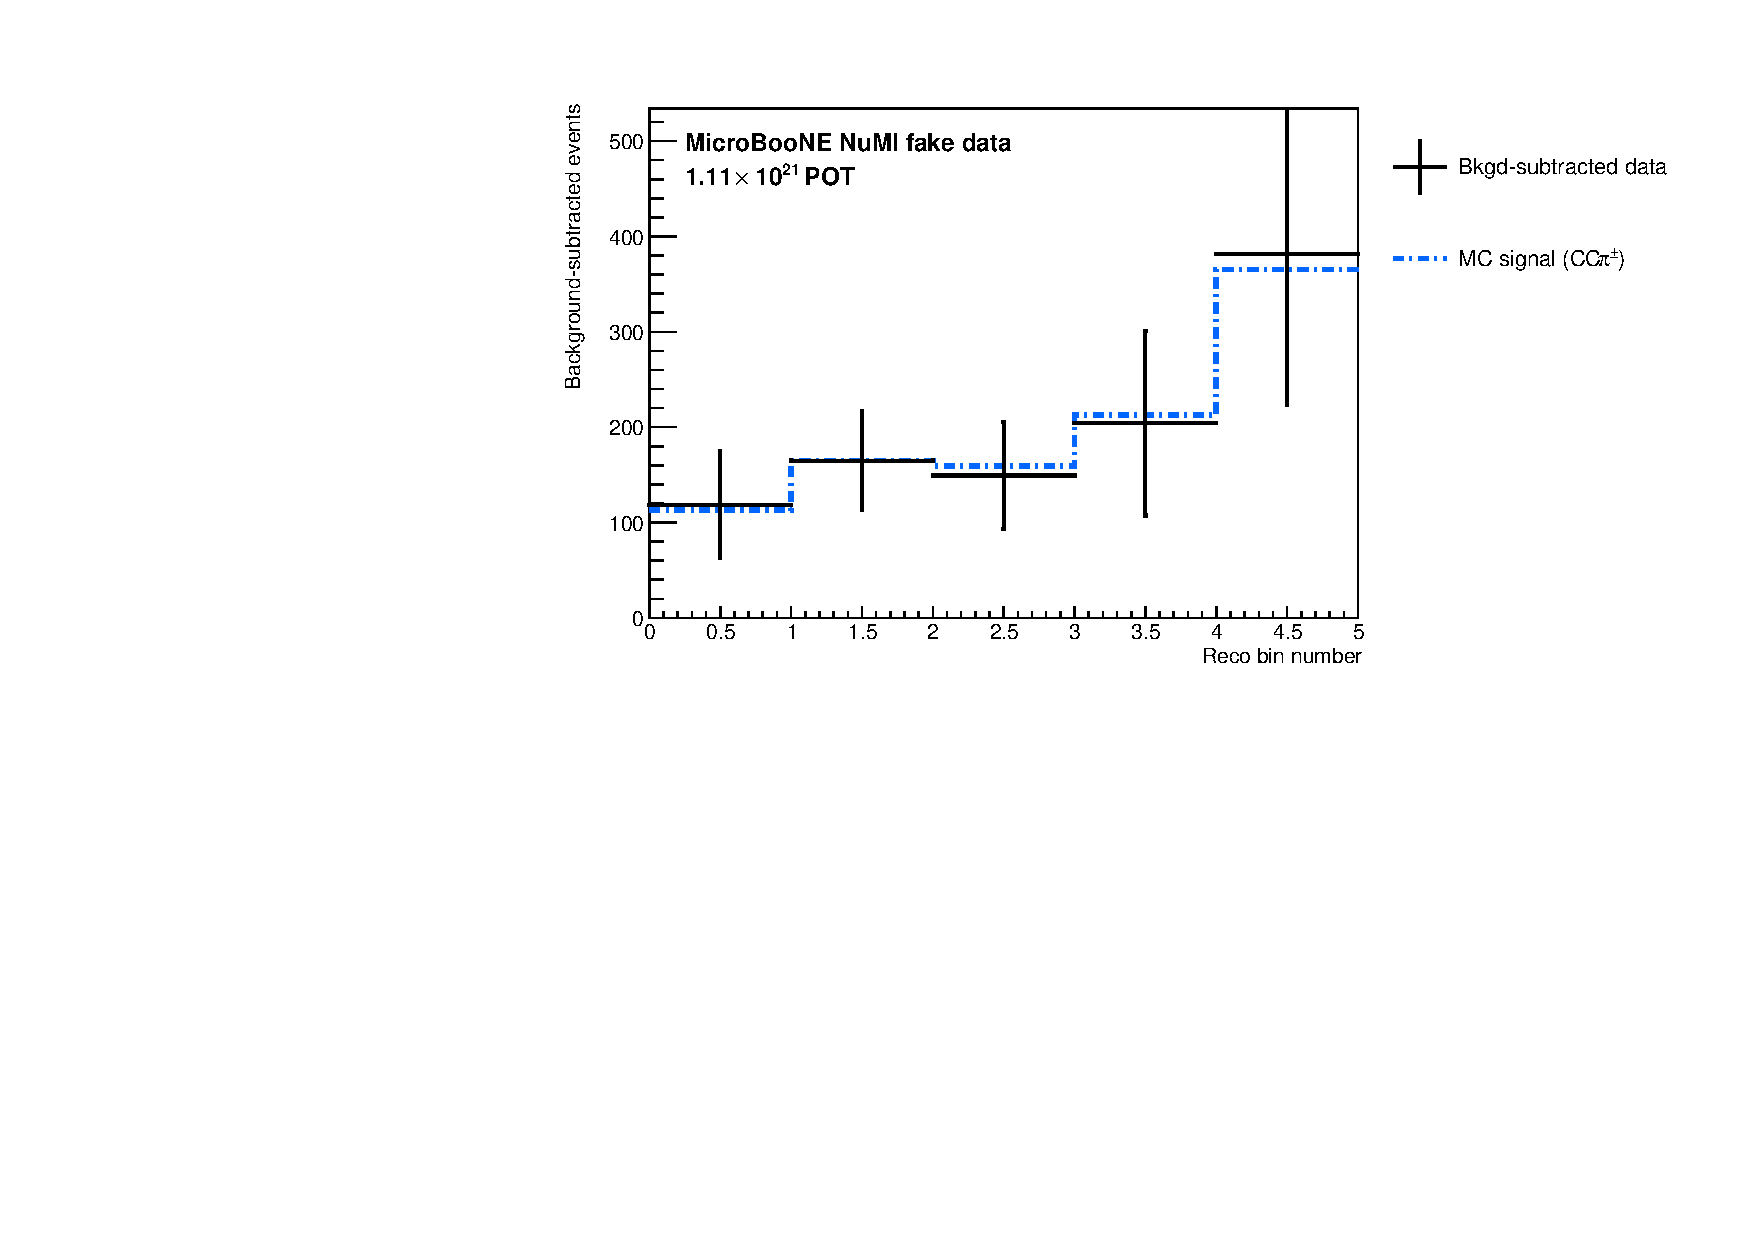
\includegraphics[width=\textwidth]{step2_bsub_costhpi_RHCFULL}\caption{$\cos\theta_\pi$}\end{subfigure}\hfill
  \begin{subfigure}[b]{0.32\textwidth}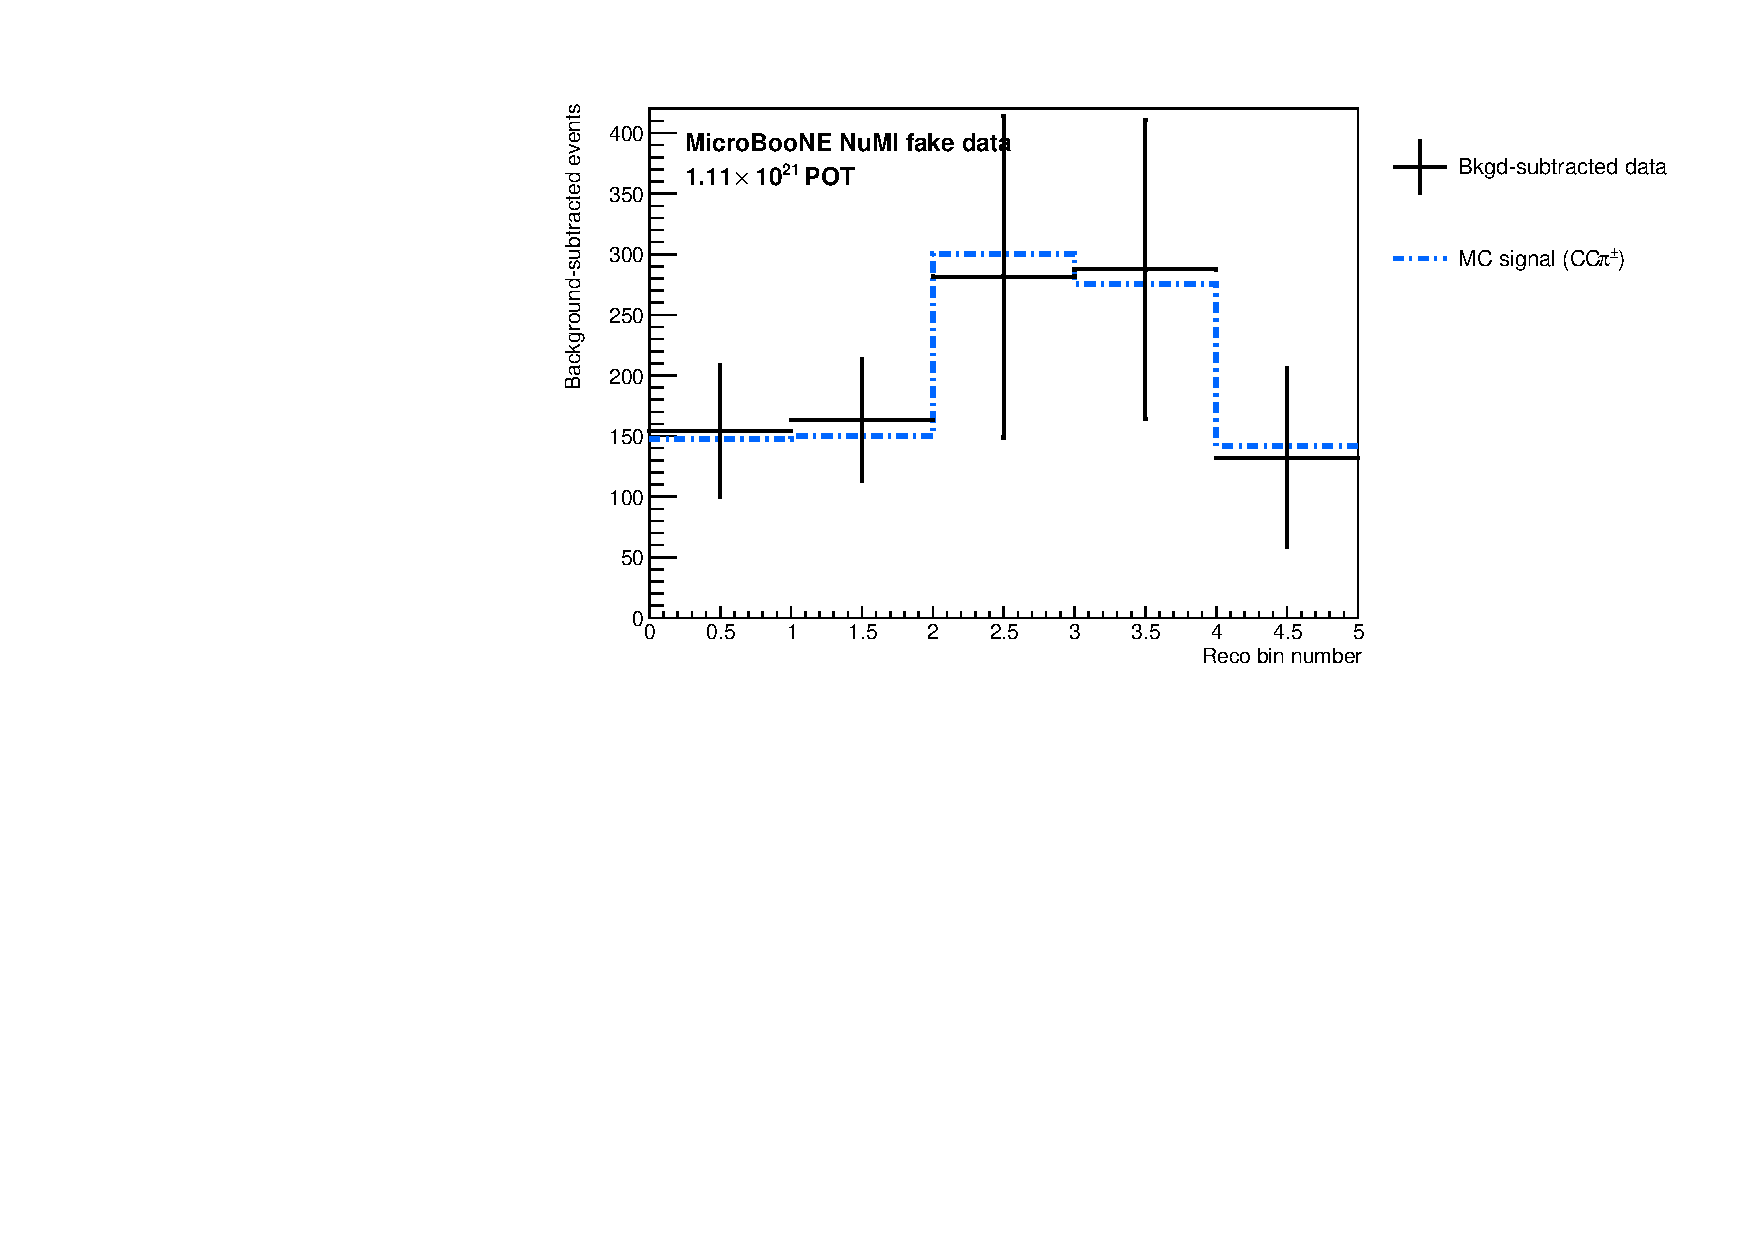
\includegraphics[width=\textwidth]{step2_bsub_thmupi_RHCFULL}\caption{$\theta_{\mu\pi}$}\end{subfigure}\hfill
  \begin{subfigure}[b]{0.32\textwidth}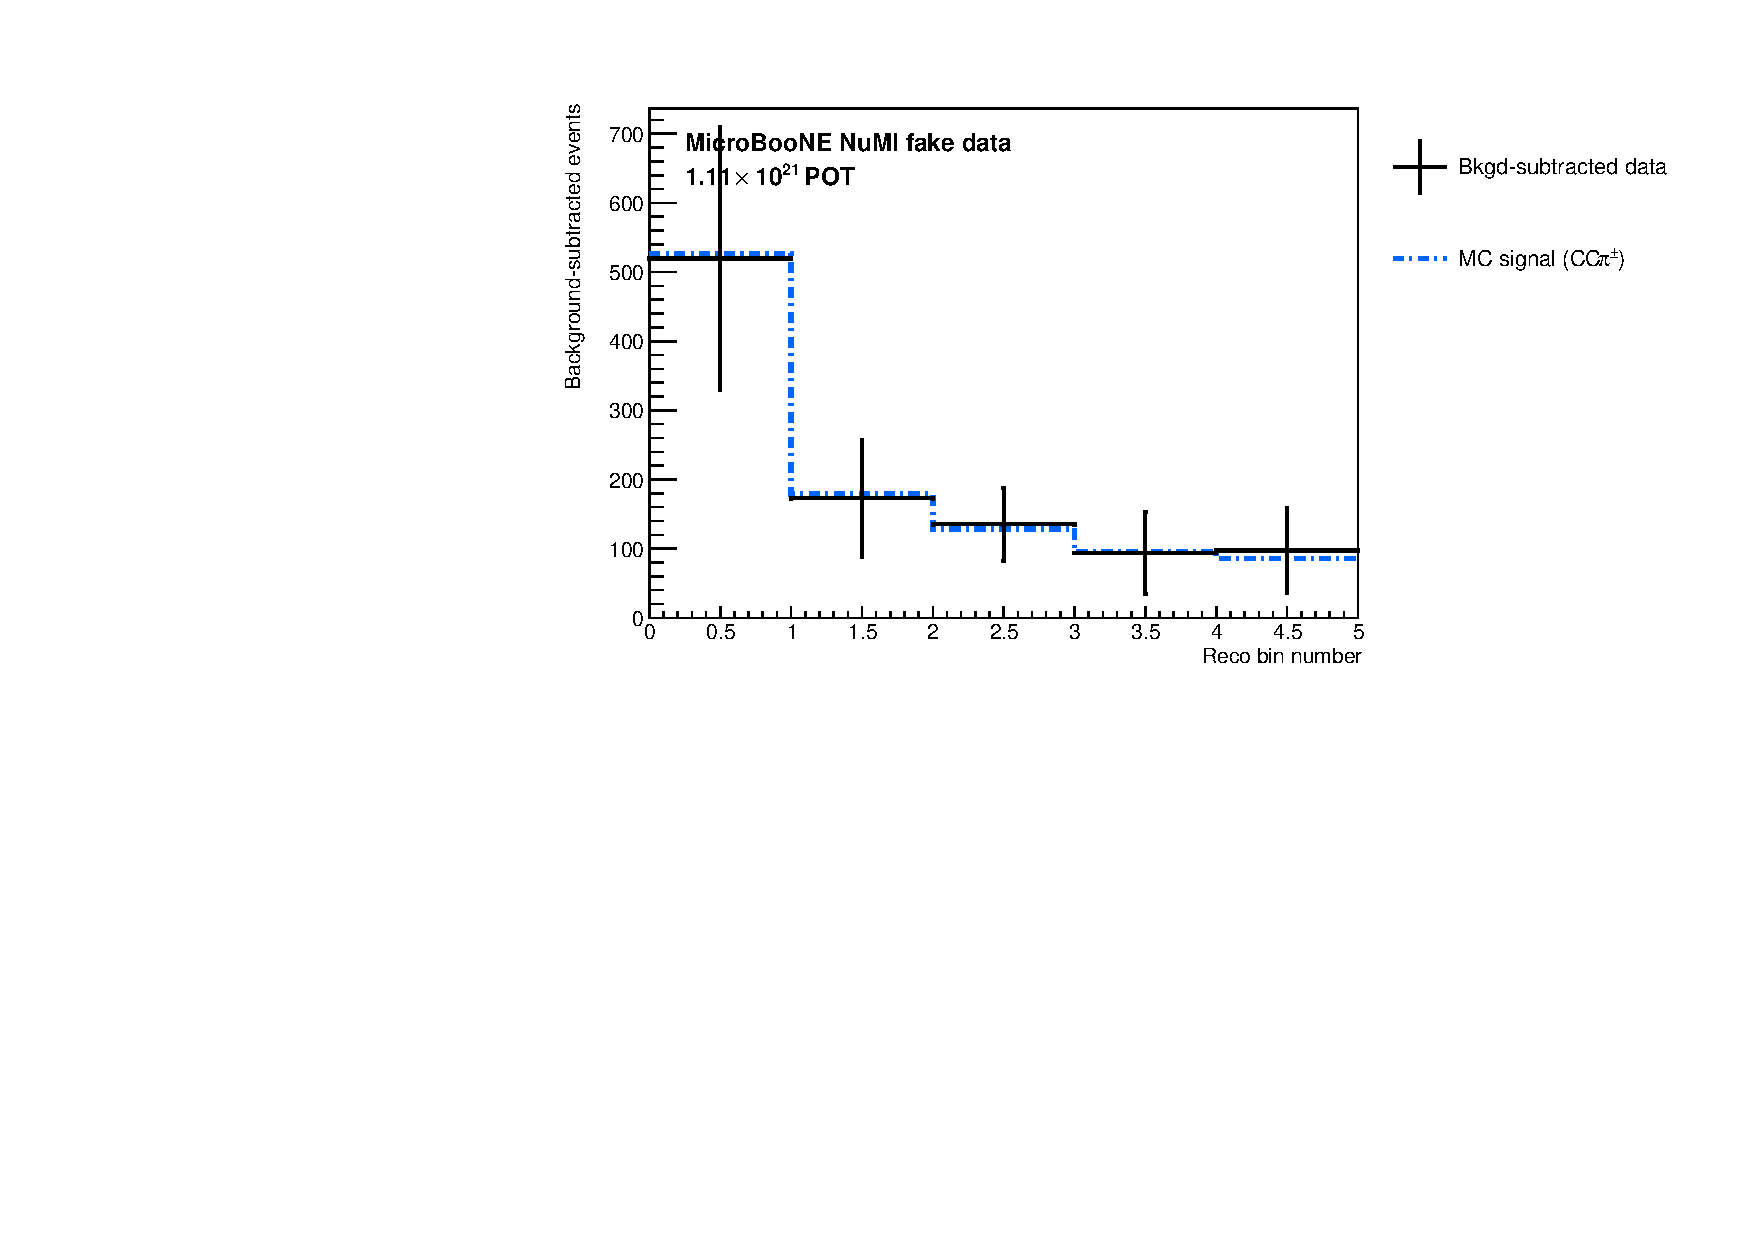
\includegraphics[width=\textwidth]{step2_bsub_thetamu_RHCFULL}\caption{$\theta_\mu$}\end{subfigure}
  \caption{Stage 2, RHC: background-subtracted data compared with the central-value MC signal.}
  \label{fig:chain_bsub_rhc}
\end{figure}



\subsection{Signal extraction}

After the event selection, the background-subtracted reco-space signal spectrum
for observable $x$ is:
\begin{equation}
  d_i^{\,\mathrm{sig}} = d_i^{\,\mathrm{data}} - b_i^{\,\nu\text{-bkg}}
                          - b_i^{\,\mathrm{EXT}} - b_i^{\,\mathrm{dirt}},
\end{equation}
where $i$ runs over reconstructed bins.

\subsection{Response matrix}
\label{sec:unfolding_resp}

Two distinct matrices are in play and it is worth separating them, since they differ
by exactly the efficiency. The \emph{migration} matrix
\begin{equation}
  M_{ij} = P(\text{reco in bin } i \,|\, \text{true in bin } j,\ \text{selected}),
  \qquad \textstyle\sum_i M_{ij} = 1,
\end{equation}
describes only where selected events move between bins. The \emph{smearceptance}
matrix additionally carries the probability of being selected at all,
\begin{equation}
  S_{ij} = \varepsilon_j\, M_{ij},
  \qquad \textstyle\sum_i S_{ij} = \varepsilon_j,
  \label{eq:smearcept}
\end{equation}
where $\varepsilon_j$ is the ratio of selected to generated signal events in true bin $j$.

It is $S$, not $M$, that enters the unfolding: the unfolder receives the smearceptance
matrix, and the efficiency of
Fig.~\ref{fig:efficiency} is recovered as its column sums. $S$ is built from selected
signal MC using the same binning on both axes. The folding relation the unfolder inverts
is therefore
\begin{equation}
  n_i^{\mathrm{reco}} = \sum_j S_{ij}\,N_j^{\mathrm{true}} + b_i,
  \qquad S_{ij}=\varepsilon_j M_{ij},
  \label{eq:folding}
\end{equation}
and the unfolded $\hat N_j^{\mathrm{true}}$ is already efficiency-corrected: no
separate division by $\varepsilon_j$ is applied afterwards (\S\ref{eq:xsec_def}).
Figure~\ref{fig:response} plots $S$ itself, exactly the matrix passed to the unfolder
(colour scale $P(\mathrm{reco}\,|\,\mathrm{true})\times\varepsilon$, so each column sums
to the efficiency of that true bin rather than to unity). The migration diagonals quoted
in this note, for example $91\%$ and $76\%$ for the two $p_\pi$ bins, are elements of the
column-normalised $M$, obtained from $S$ by dividing each column by its sum; they are
not read off the
colour scale of Fig.~\ref{fig:response}.

\subsection{Regularised unfolding: the bias--variance trade-off}
\label{sec:unfmethods}

Unfolding inverts the folding relation $\vec{m} = A\,\vec{s} + \vec{b}$ to estimate the
true signal spectrum $\vec{s}$ from the measured $\vec{m}$. The naive inverse
$A^{-1}(\vec{m}-\vec{b})$ is unbiased but useless: bin migration makes $A$ nearly
singular, so its inverse amplifies statistical fluctuations into large, anticorrelated
bin-to-bin oscillations. Every practical method therefore \emph{regularises}, trading
a small, controlled bias for a large reduction in variance. This analysis uses two
complementary methods.

\paragraph{Wiener-SVD (primary).} Diagonalising the response with an SVD, each mode $k$
is weighted by the Wiener filter $W_k=\sigma_k^2/(\sigma_k^2+N_k)$; the
minimum-mean-squared-error weighting, $\simeq 1$ for well-measured modes and $\to 0$ for
noise-dominated ones, so no regularisation strength is tuned by hand. The price is a
\emph{known} linear bias: the unfolded data estimates not $\vec{s}$ but the smeared
spectrum $A_C\vec{s}$, where the additional-smearing matrix $A_C$ is published so that
every theory prediction is smeared by the same $A_C$ before comparison.

\paragraph{D'Agostini iterative Bayesian~\cite{dagostini} (cross-check).} Bayes' theorem inverts the
migration, $P(C_j|E_i)=R_{ij}\pi_j/\sum_l R_{il}\pi_l$, and the unfolded estimate is
$\hat{s}_j=\varepsilon_j^{-1}\sum_i P(C_j|E_i)(m_i-b_i)$. The MC prior $\pi_j$ is updated
with the result and iterated; the \emph{number of iterations} is the regularisation knob
(few $\Rightarrow$ prior-biased, many $\Rightarrow$ noisy). It carries no $A_C$, so its
integral is essentially unbiased and theory is compared raw.

\begin{table}[H]\centering\small
\caption{Trade-offs of the two unfolding methods. Neither is ``more correct''; they make
  complementary choices about how to trade bias for variance and how to expose the
  residual bias.}
\label{tab:unfcompare}
\begin{tabular}{lll}
\toprule
 & \textbf{Wiener-SVD} & \textbf{D'Agostini (iter.\ Bayes)} \\
\midrule
Regularisation    & Wiener filter (automatic, from S/N) & Iteration count $n$ (chosen) \\
Residual bias     & Explicit $A_C$, published           & Implicit; set by early stopping \\
Result integral   & Suppressed, observable-dependent    & Essentially unbiased (physical) \\
Theory comparison & Smear theory by $A_C$               & Raw theory \\
Positivity        & Not guaranteed                      & Guaranteed for positive input \\
Uncertainties     & Closed-form, linear                 & Correlated across iters.; needs care \\
\bottomrule
\end{tabular}
\end{table}

Wiener-SVD is the primary result, for its objective regularisation and its explicit,
reportable bias $A_C$; D'Agostini serves as the quantitative cross-check
(\suppref{Sec.}{sec:crosschecks}), where its flat,
iteration-stable integral, $23$--$31\%$ above Wiener-SVD (config-dependent), is
consistent with the observable-to-observable spread of the Wiener-SVD integrated cross
sections (Table~\ref{tab:sigint_all}) being the $A_C$ smearing rather than a physical or
acceptance effect; the row sums of \S\ref{sec:ac_rowsums} establish that directly. That is all it can establish here: with
central-value pseudo-data and the same central value as its prior, D'Agostini returns its
prior, so its flatness and iteration stability are guaranteed and say nothing about its
bias on a different truth. The alternative-generator fake-data pass of
\S\ref{sec:limitations} would make it a real test.

\subsection{Wiener-SVD unfolding}

The primary method is Wiener-SVD~\cite{wienervsd}. Every released result is produced
by the Wiener-SVD unfolder of the XSecAnalyzer framework~\cite{xsec_analyzer,uboone_tki}:
Cholesky whitening of the data covariance, regularisation inside the SVD of
$R\,C^{-1}$, and the Wiener filter of Eq.~3.24 of Ref.~\cite{wienervsd}, whose
strength is set by the data covariance rather than by hand. The regularisation matrix
$C$ is the second-derivative operator on the \emph{density}, corrected for the
non-uniform bin widths, with one-sided first-derivative rows at the ends. The
width correction matters: on these binnings, whose widths vary by up to a factor of $14$ ($\cos\theta_\mu$; $10$ for
$\theta_\mu$, $6$ for $p_\mu$), a uniform-grid stencil penalises the density's curvature by the wrong weights
and drives $A_C$ towards rank one, so that every model is smeared onto one shape and
the measurement carries no shape information (\suppref{Sec.}{sec:thetavar}). A
standalone replica of the unfolder exists for cross-pipeline checks; it imports the framework's
covariance because it throws no universes, and with a statistics-only covariance it
under-regularises and over-corrects the integral by $\sim26\%$, which is why it is not
used for any released number.

The differential cross section is:
\begin{equation}
  \left.\frac{d\sigma}{dx}\right|_j
  = \frac{\hat{N}_j^{\,\mathrm{true}}}
         {\Delta x_j \cdot \Phi_{\mathrm{total}} \cdot N_{\mathrm{Ar}}},
  \label{eq:xsec_def}
\end{equation}
where $\hat{N}_j^{\,\mathrm{true}}$ is the Wiener-SVD estimate of the true signal count
in true bin $j$ obtained by inverting Eq.~\eqref{eq:folding},
$\Phi_{\mathrm{total}} = \Phi_{\mathrm{per\,POT}} \times T_{\mathrm{POT}}$
is the total integrated flux, and $N_{\mathrm{Ar}}$ is the number of argon
target nuclei in the FV. Because the response supplied to the unfolder is the
smearceptance matrix $S=\varepsilon M$, the efficiency correction is part of the
inversion and \emph{no explicit} $1/\varepsilon_j$ appears here (one would apply the
correction twice). The implementation forms each bin as
$\hat N_j^{\,\mathrm{true}}/(\mathrm{conv}\cdot\Delta x_j)$ with the
events-to-cross-section conversion $\mathrm{conv} = N_{\mathrm{Ar}}\,\Phi_{\mathrm{total}}/10^{-38}$
and applies no further efficiency factor. The per-configuration inputs at the final
exposures are:

\begin{center}\small
\begin{tabular}{lccc}
\toprule
Quantity & FHC & RHC & Combined \\
\midrule
$N_{\mathrm{Ar}}$ (FV, dead-region excluded) & \multicolumn{3}{c}{$8.710\times10^{29}$} \\
Flux constant $\phi$ ($E_\nu>60$~MeV; $10^{-10}$~cm$^{-2}$/POT) & $6.81159$ & $6.44646$ & $6.60865$ \\
Data POT ($10^{20}$)                         & $8.857$ & $11.082$ & $19.939$ \\
Integrated flux $\Phi_{\mathrm{total}} = \phi\times$POT ($10^{11}$~cm$^{-2}$) & $6.033$ & $7.144$ & $13.177$ \\
$\mathrm{conv} = N_{\mathrm{Ar}}\,\Phi_{\mathrm{total}}/10^{-38}$ (events per $10^{-38}$~cm$^2$/Ar) & $5255$ & $6223$ & $11478$ \\
\bottomrule
\end{tabular}
\end{center}

\noindent An integrated cross section is computed as the width-weighted sum,
\begin{equation}
  \sigma_{\mathrm{int}} = \sum_j \left.\frac{d\sigma}{dx}\right|_j \Delta x_j .
\end{equation}
It is \emph{not} required to agree between observables: the Wiener-SVD result estimates
$A_C\,x_{\mathrm{true}}$ and $A_C$ is not norm preserving, so $\sigma_{\mathrm{int}}$ is
observable-dependent (\S\ref{sec:ac_rowsums}). The observable-independent total is the
one-bin total of \S\ref{sec:total_xsec}.

\subsection{Reconstructed spectra and response matrices}

Figure~\ref{fig:reco_spectra} shows the background-subtracted reco-space signal
spectra for all six observables, overlaid with the MC signal prediction and the
individual background components.

\begin{figure}[H]
  \centering
  \begin{subfigure}[b]{0.32\textwidth}
    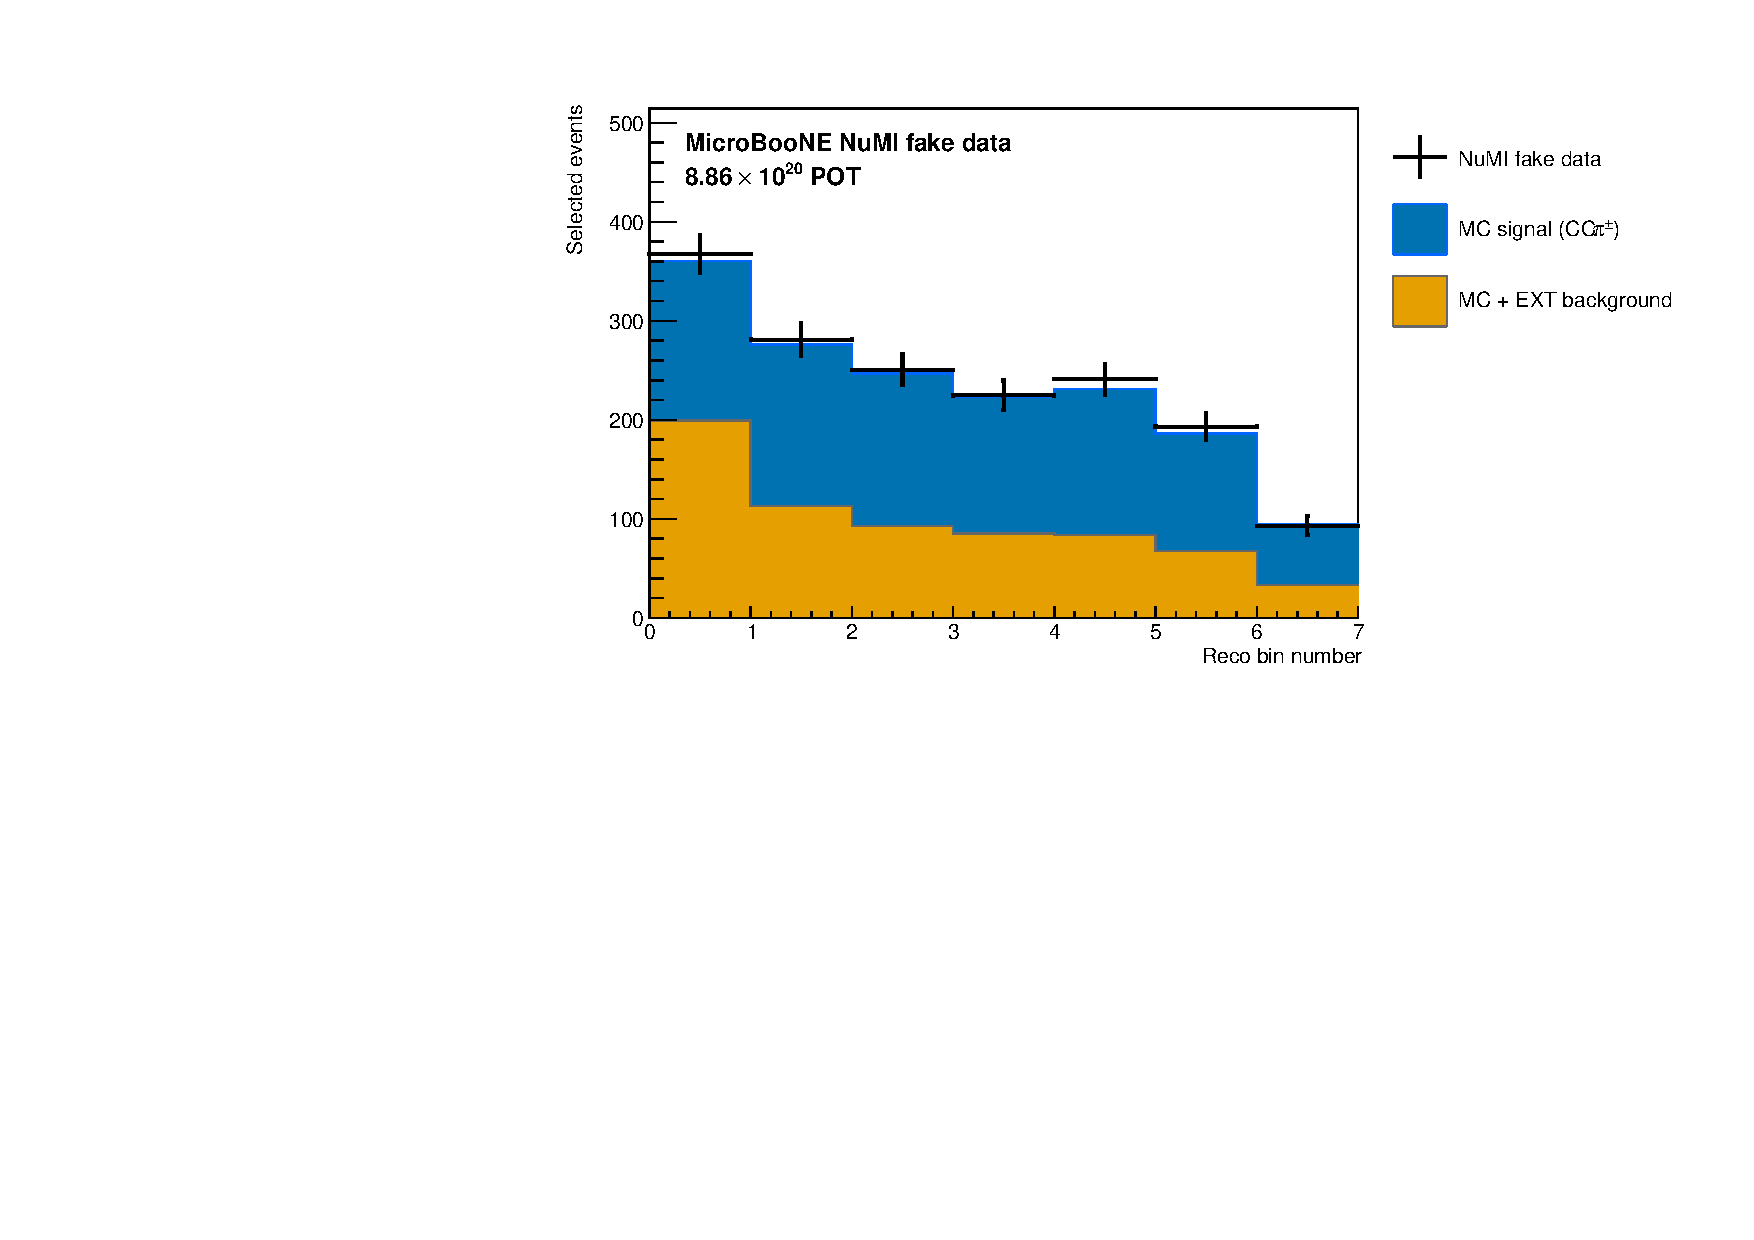
\includegraphics[width=\textwidth]{fw_reco_pmu}
    \caption{$p_\mu$}
  \end{subfigure}
  \hfill
  \begin{subfigure}[b]{0.32\textwidth}
    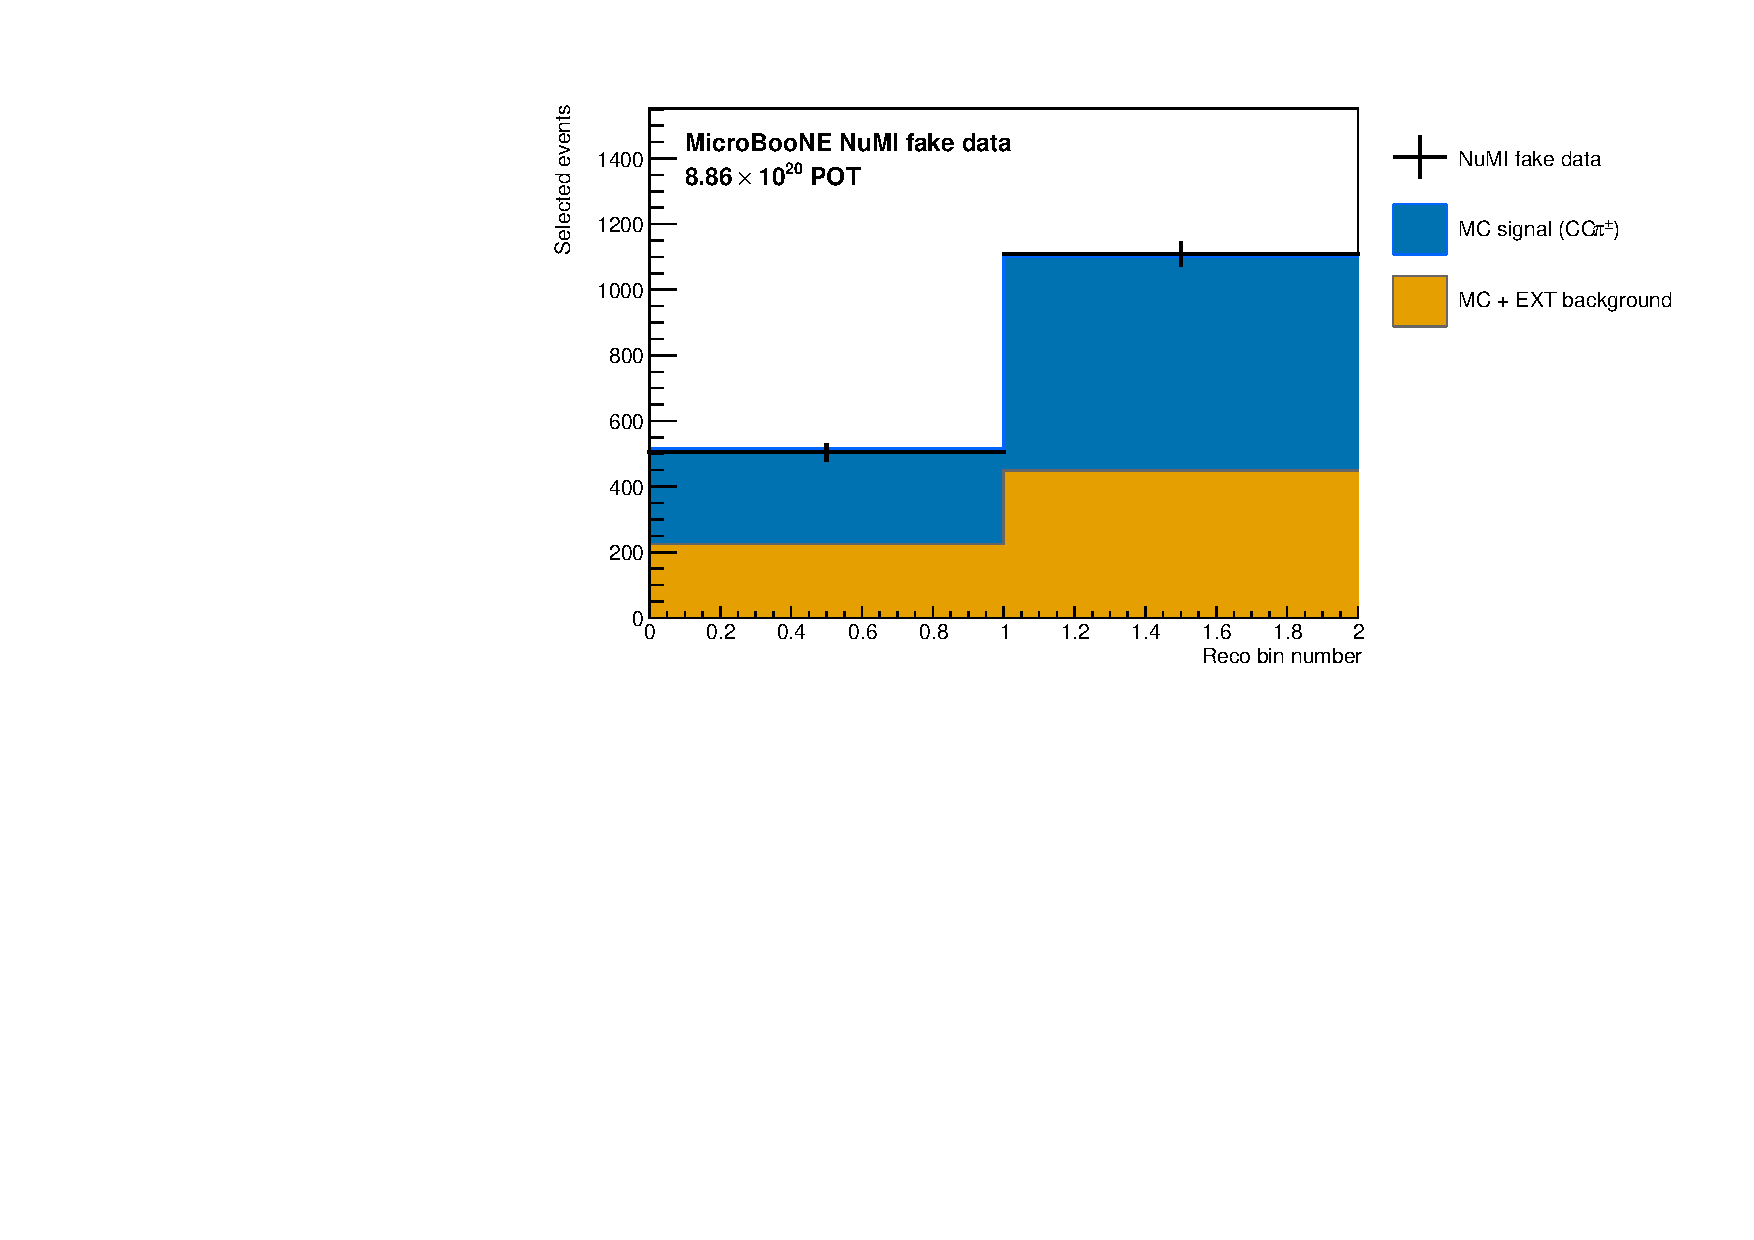
\includegraphics[width=\textwidth]{fw_reco_ppi}
    \caption{$p_\pi$}
  \end{subfigure}
  \hfill
  \begin{subfigure}[b]{0.32\textwidth}
    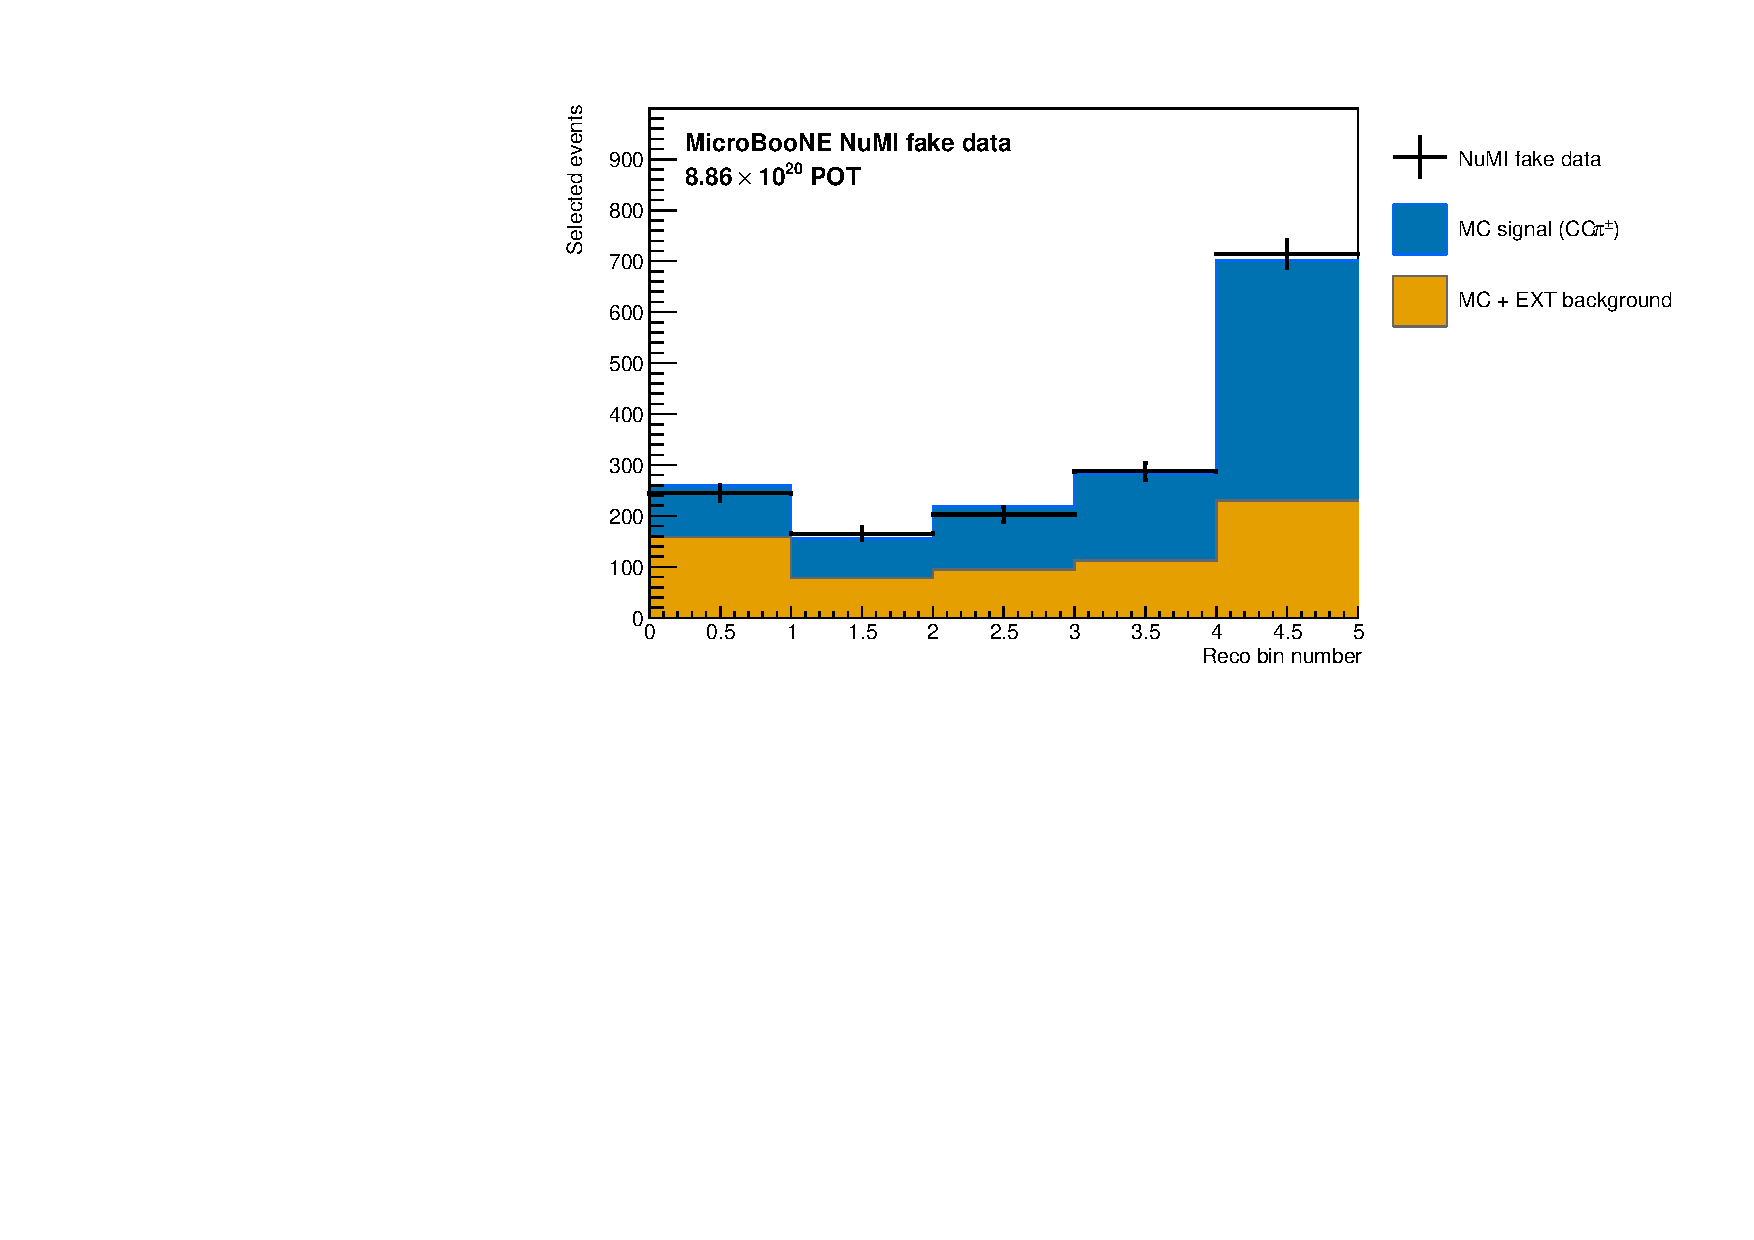
\includegraphics[width=\textwidth]{fw_reco_costhmu}
    \caption{$\cos\theta_\mu$}
  \end{subfigure}\\[6pt]
  \begin{subfigure}[b]{0.32\textwidth}
    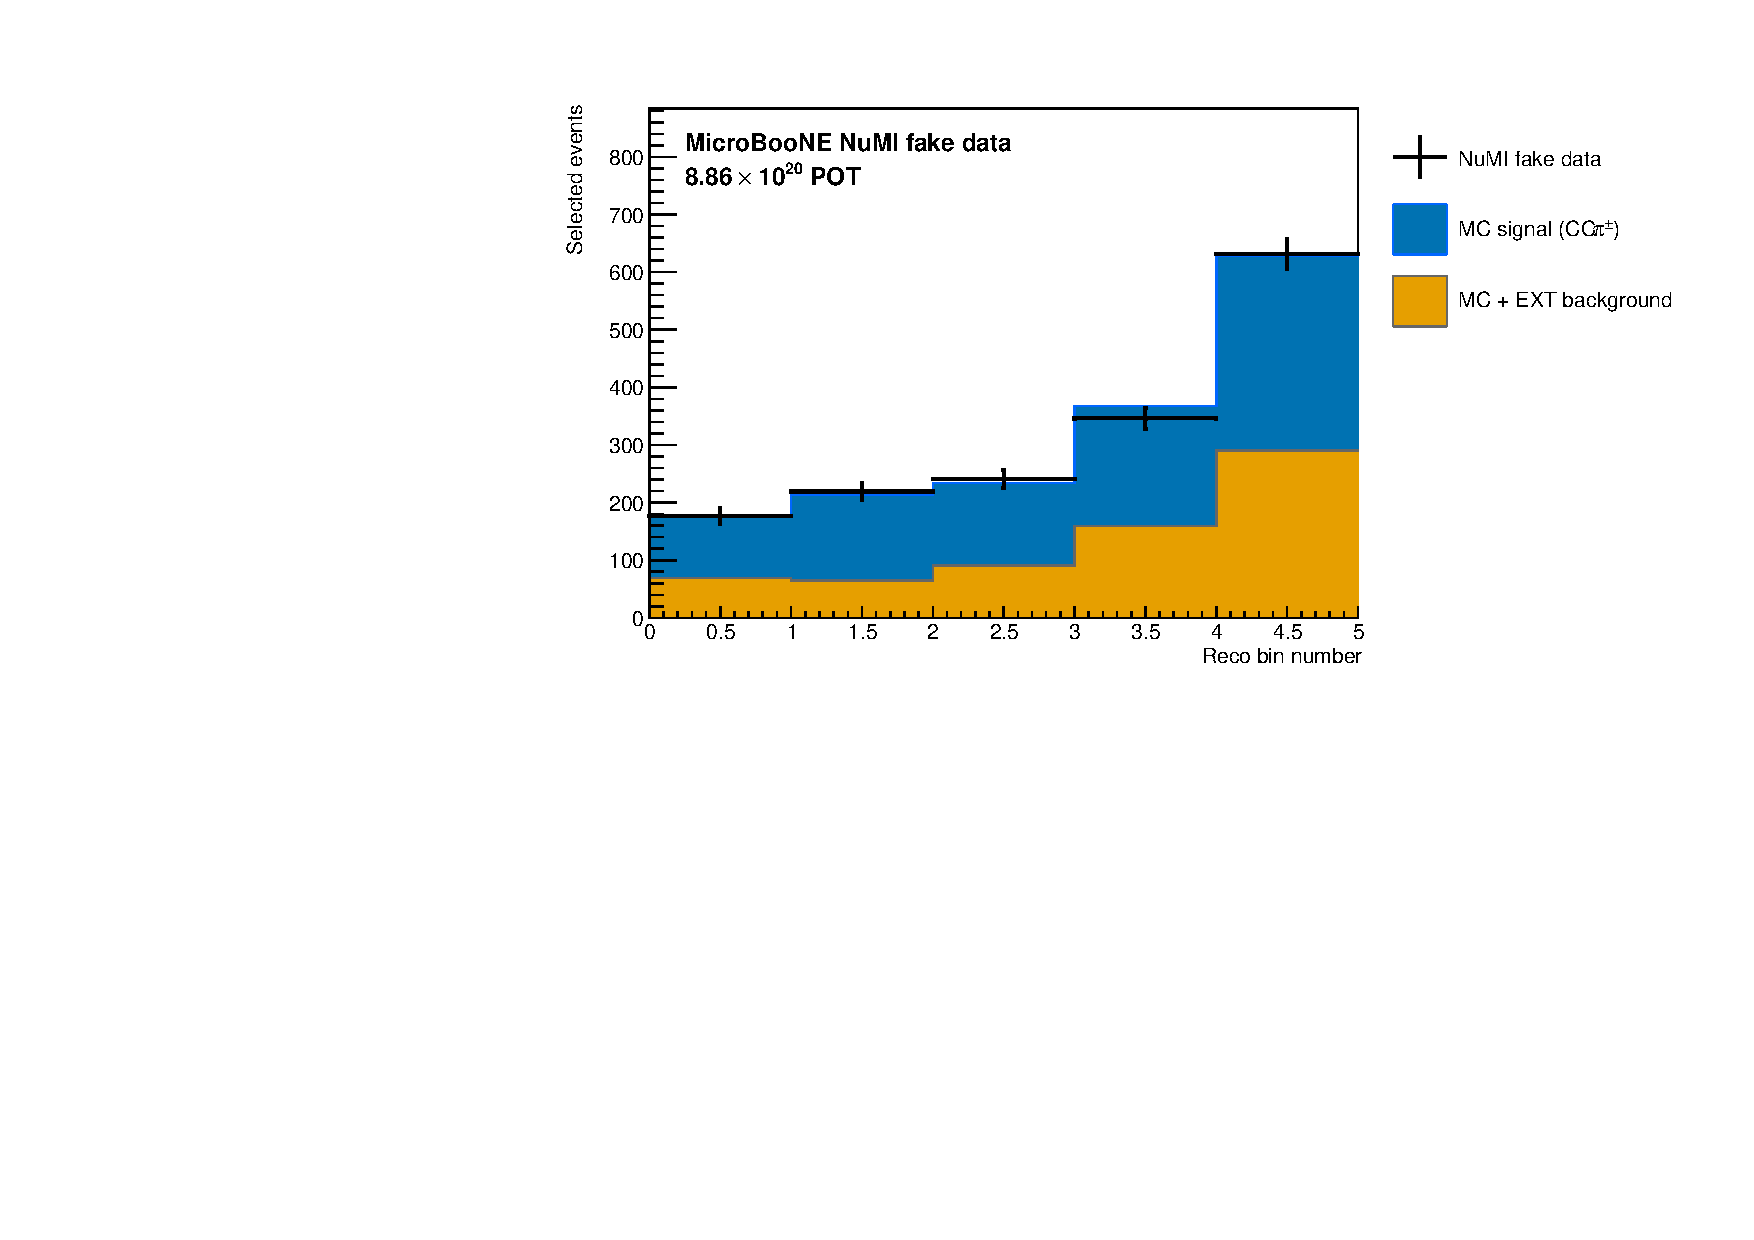
\includegraphics[width=\textwidth]{fw_reco_costhpi}
    \caption{$\cos\theta_\pi$}
  \end{subfigure}
  \hfill
  \begin{subfigure}[b]{0.32\textwidth}
    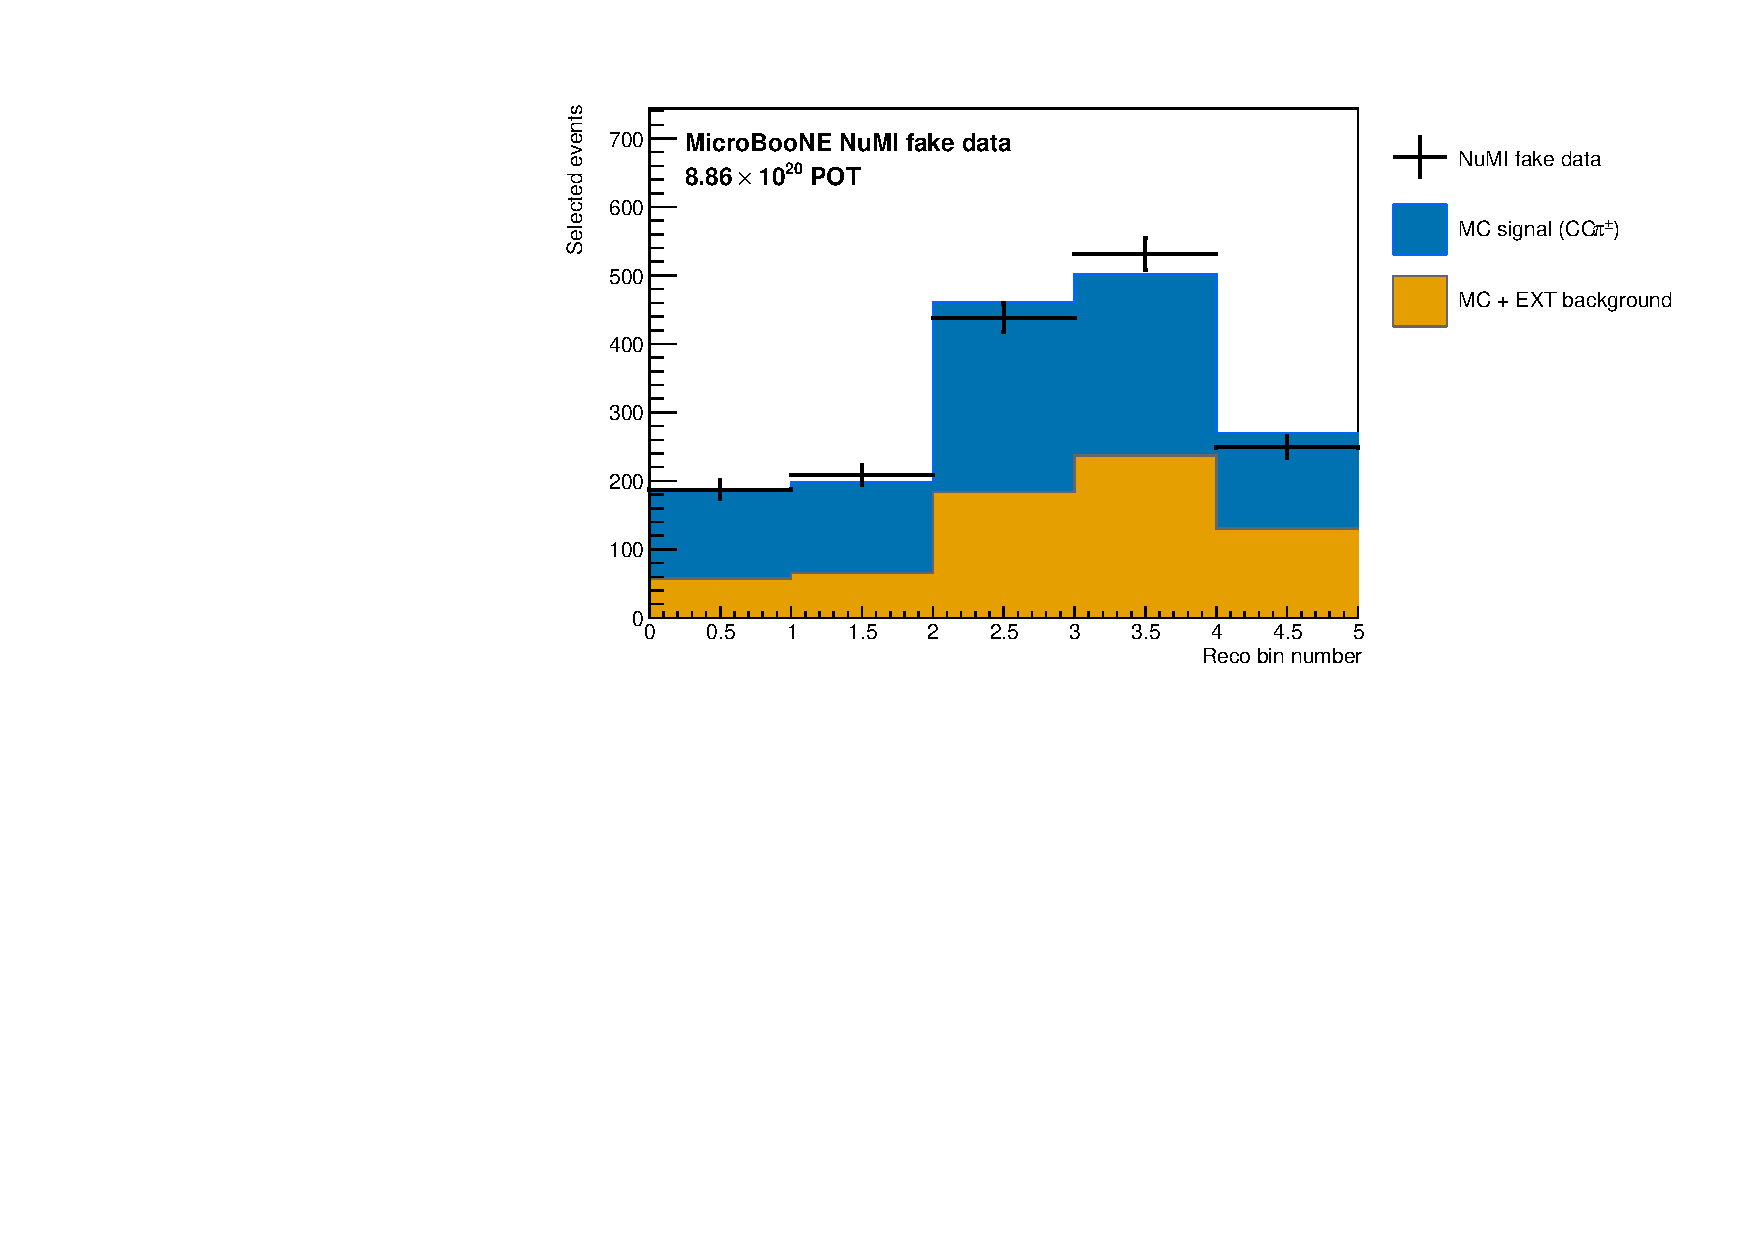
\includegraphics[width=\textwidth]{fw_reco_thmupi}
    \caption{$\theta_{\mu\pi}$}
  \end{subfigure}
  \hfill
  \begin{subfigure}[b]{0.32\textwidth}
    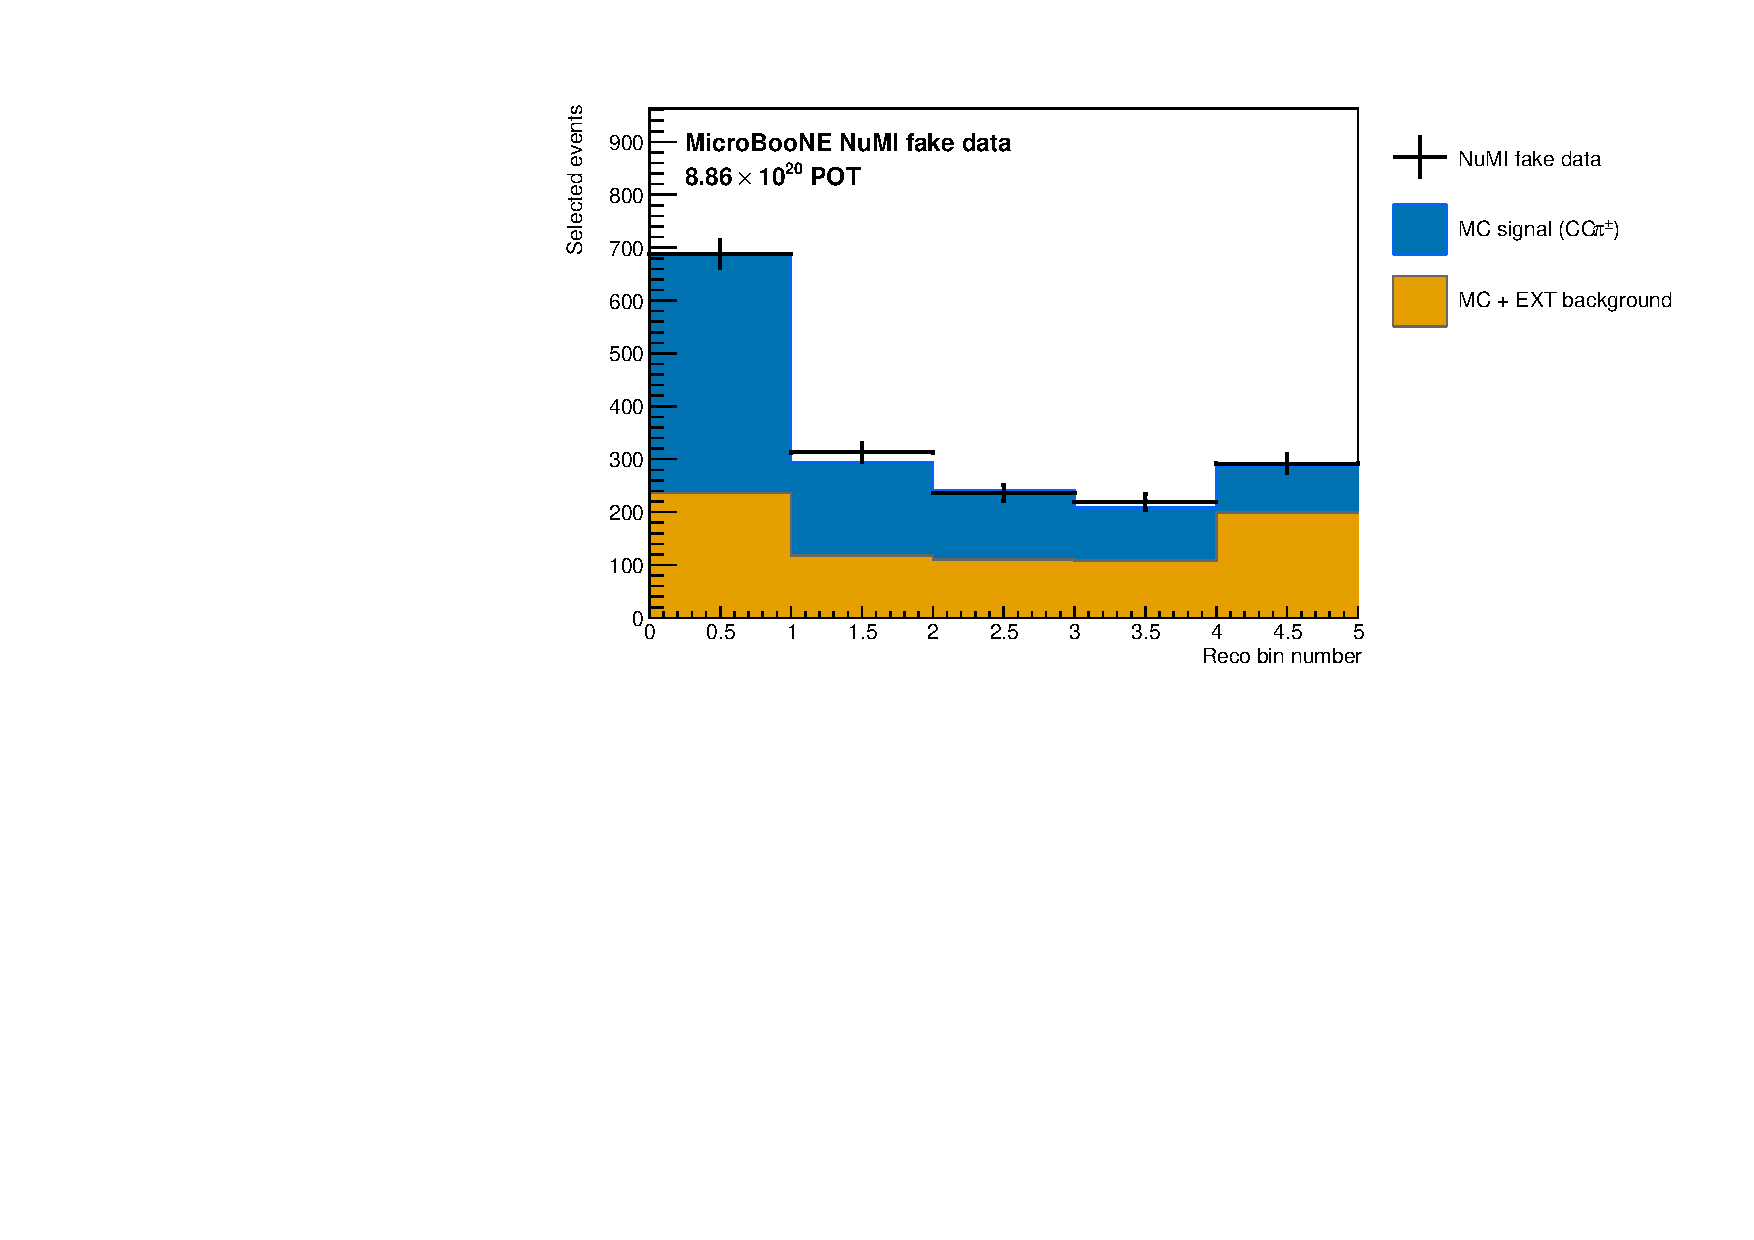
\includegraphics[width=\textwidth]{fw_reco_thetamu}
    \caption{$\theta_\mu$}
  \end{subfigure}
  \caption{Reconstructed-space spectra at the final cut for all six observables,
    FHC full exposure (Runs~1$+$2$+$4$+$5): Poisson-thrown central-value fake data
    (black points), stacked signal (blue), beam background (orange), dirt (green),
    and EXT (grey).  The fake data is drawn from the central-value Monte Carlo and so
    agrees with the stacked prediction by construction (a reco-level self-closure);
    the differential results and their closure against the $A_C$-smeared truth are
    shown in Fig.~\ref{fig:dsigma_current}.}
  \label{fig:reco_spectra}
\end{figure}

\begin{figure}[H]
  \centering
  \begin{subfigure}[b]{0.32\textwidth}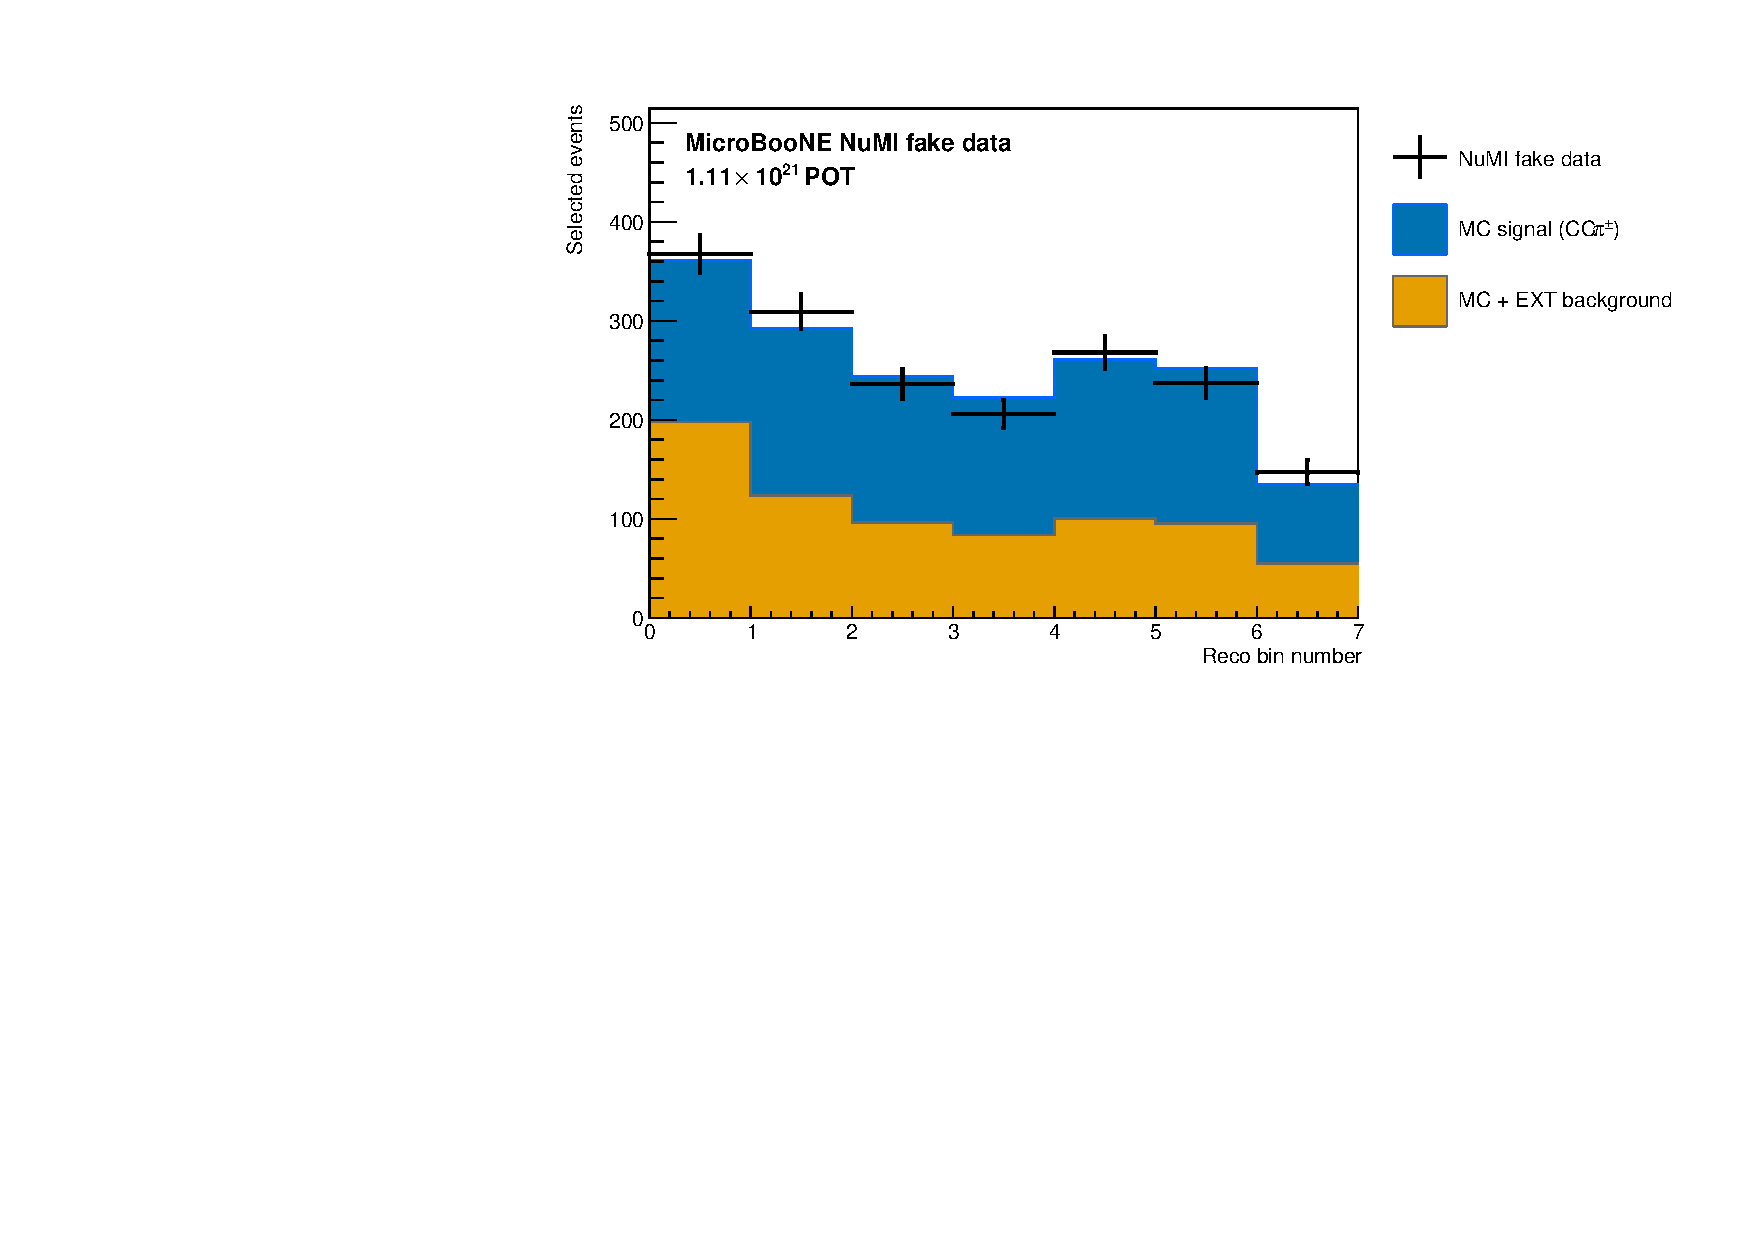
\includegraphics[width=\textwidth]{fw_reco_rhc_pmu}\caption{$p_\mu$}\end{subfigure}\hfill
  \begin{subfigure}[b]{0.32\textwidth}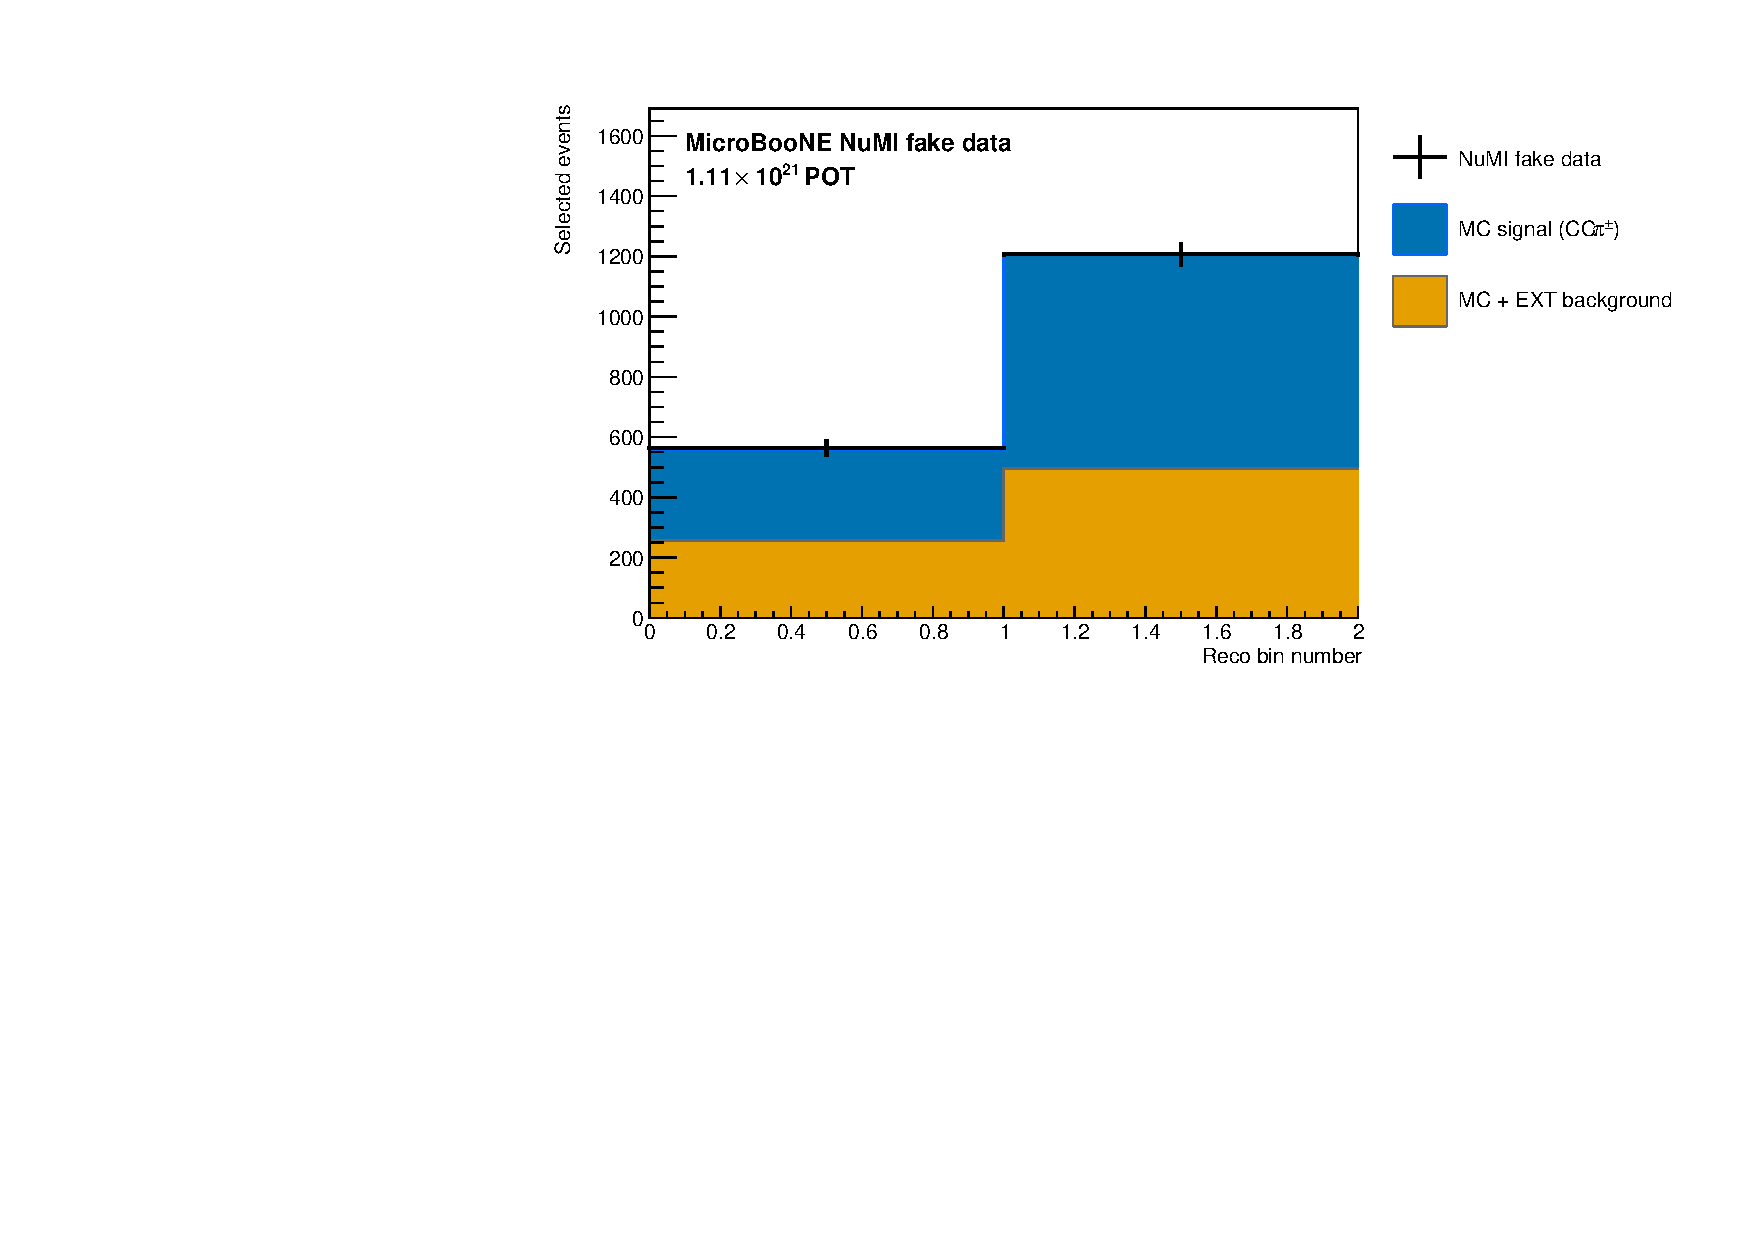
\includegraphics[width=\textwidth]{fw_reco_rhc_ppi}\caption{$p_\pi$}\end{subfigure}\hfill
  \begin{subfigure}[b]{0.32\textwidth}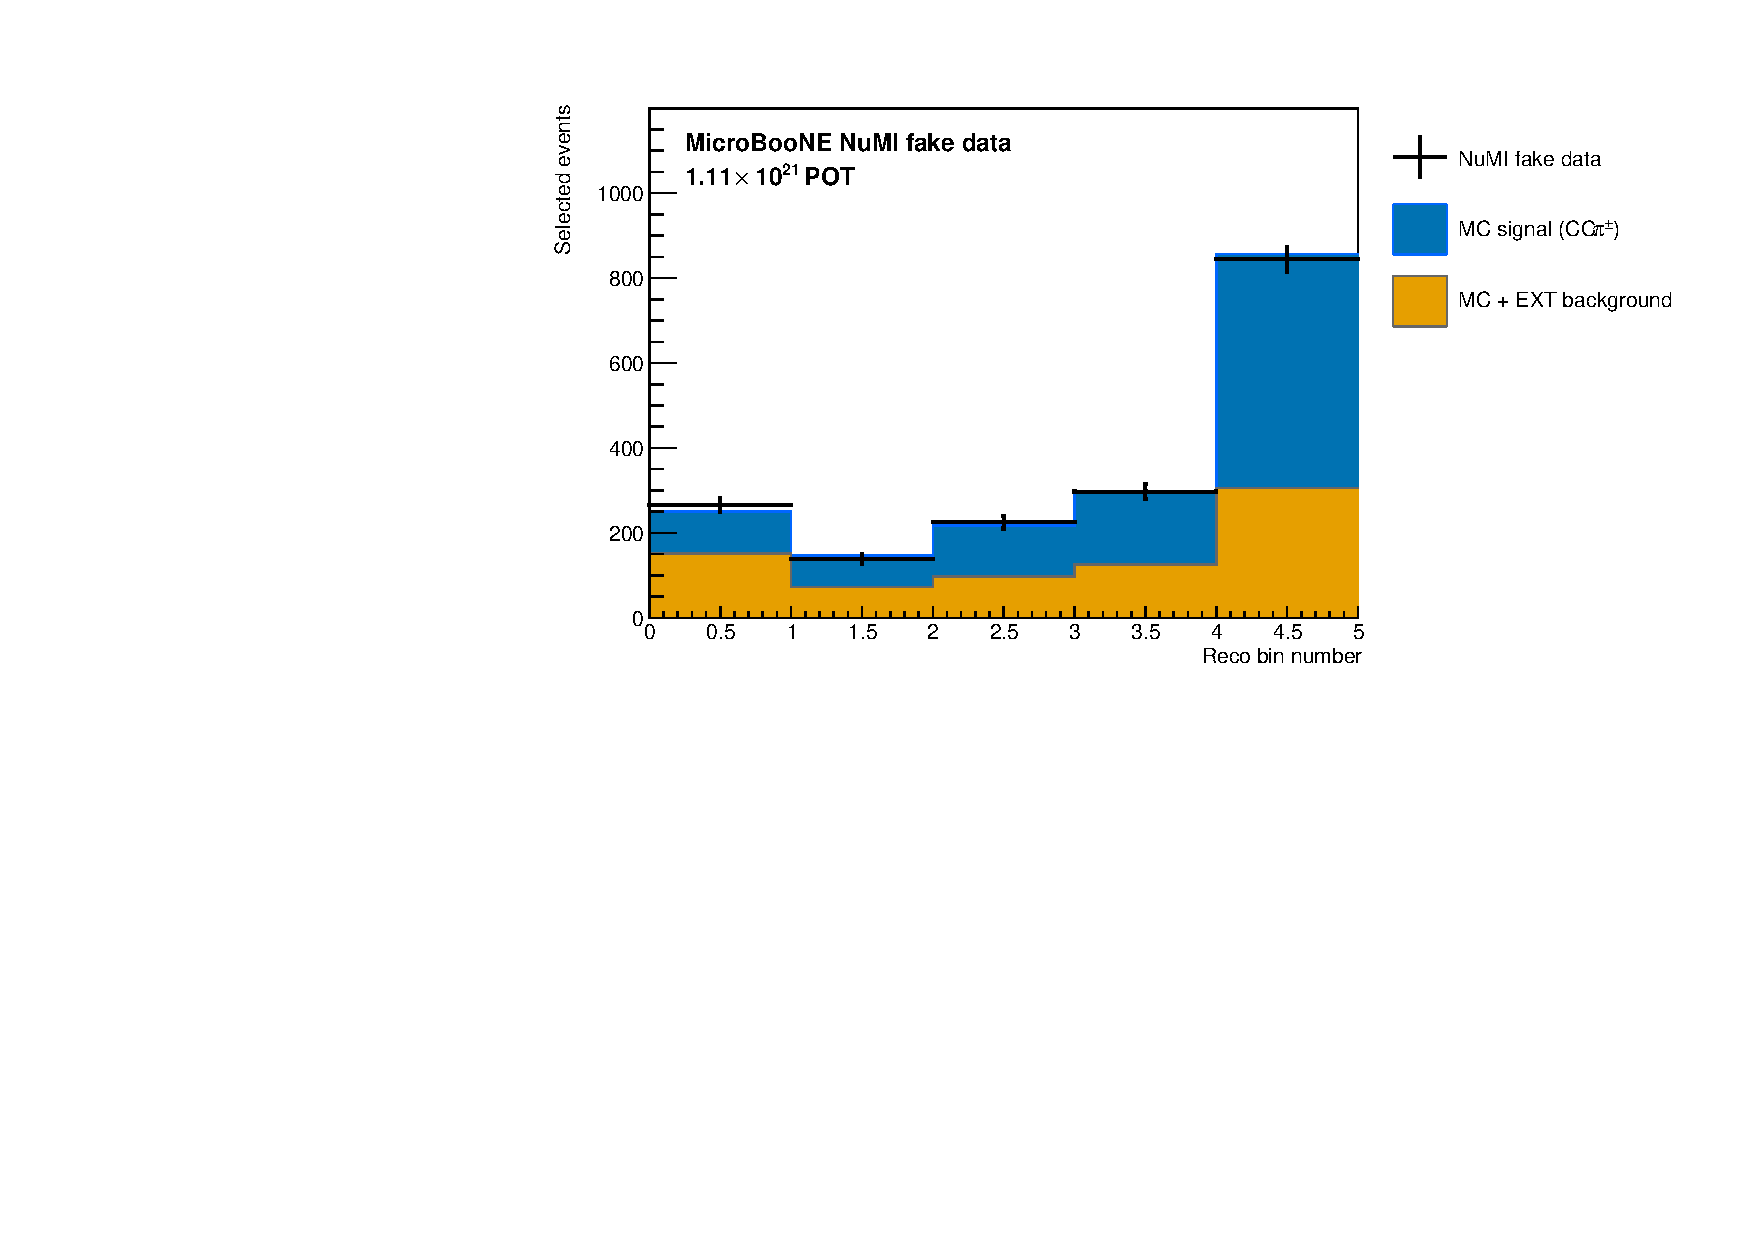
\includegraphics[width=\textwidth]{fw_reco_rhc_costhmu}\caption{$\cos\theta_\mu$}\end{subfigure}\\[6pt]
  \begin{subfigure}[b]{0.32\textwidth}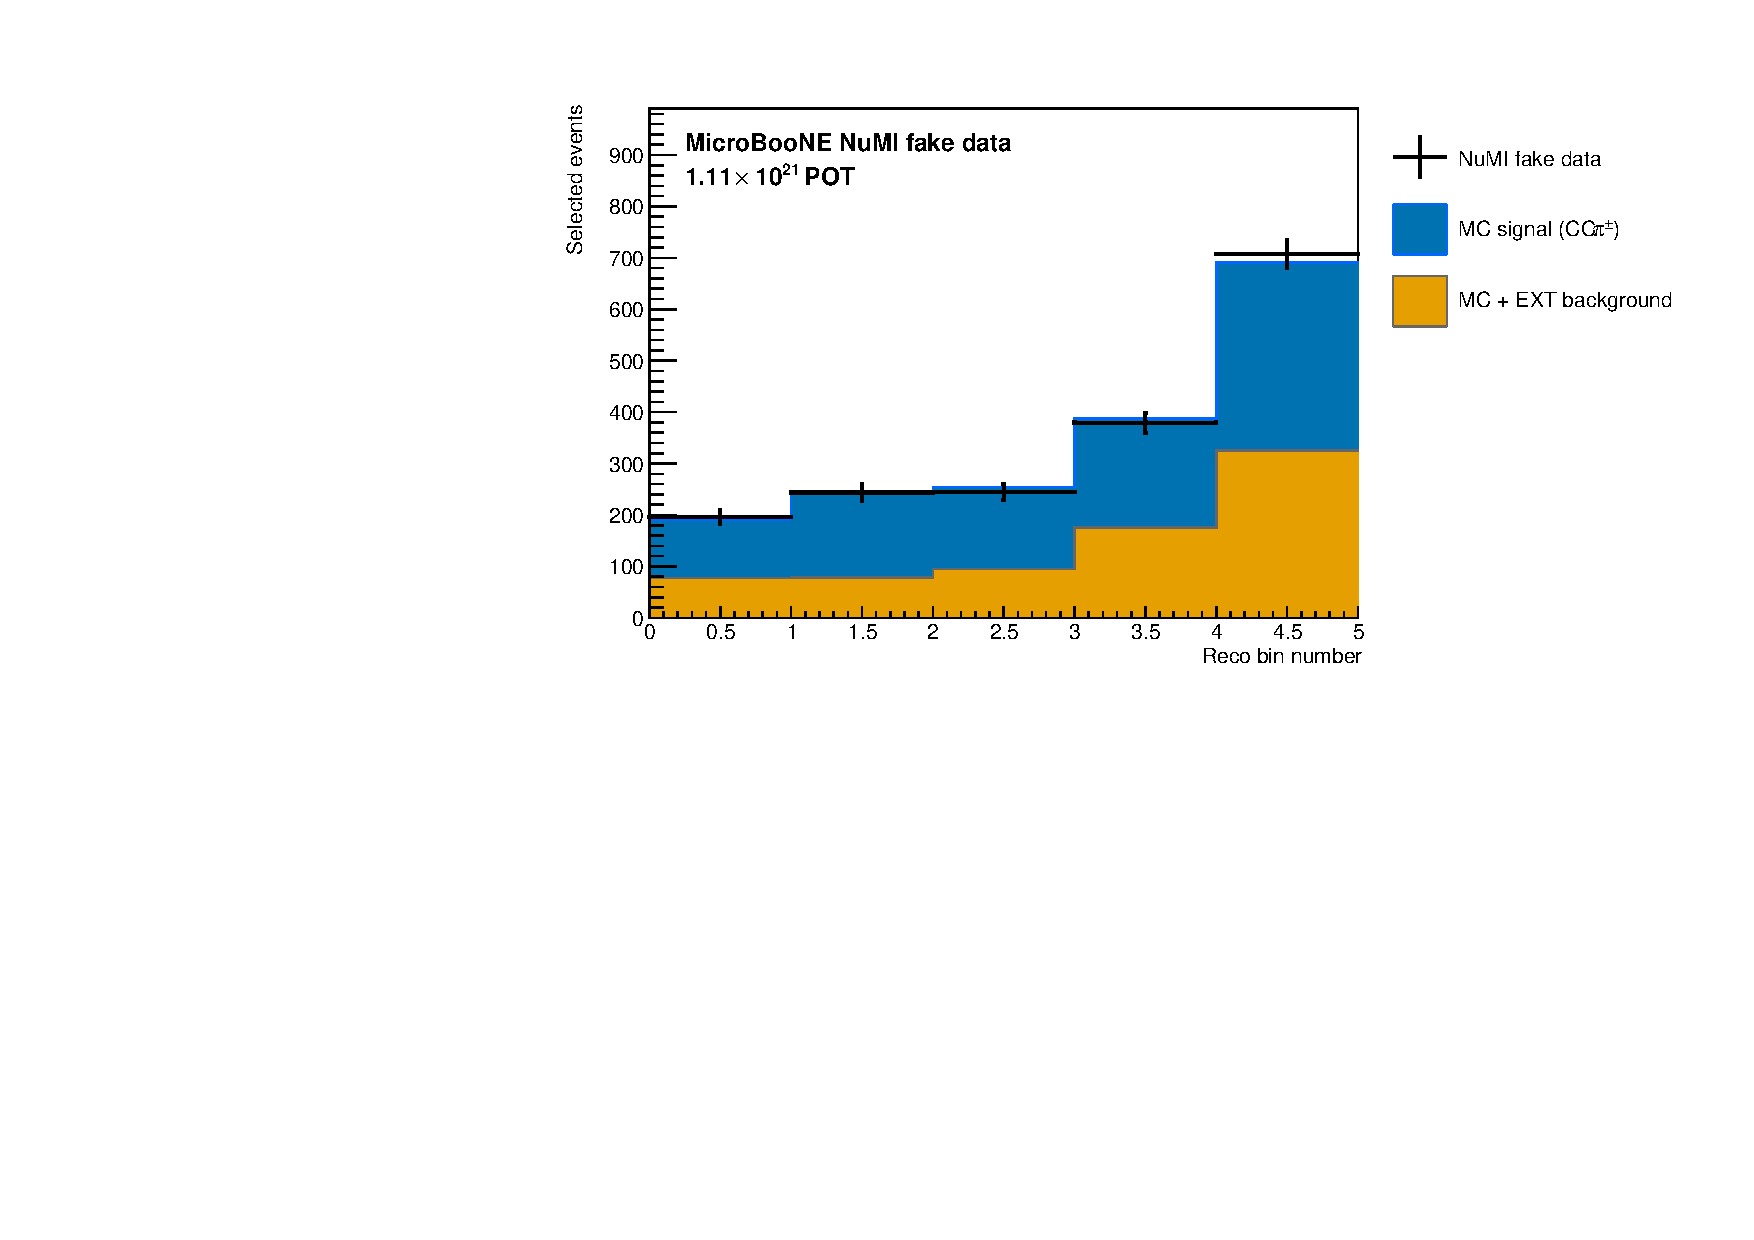
\includegraphics[width=\textwidth]{fw_reco_rhc_costhpi}\caption{$\cos\theta_\pi$}\end{subfigure}\hfill
  \begin{subfigure}[b]{0.32\textwidth}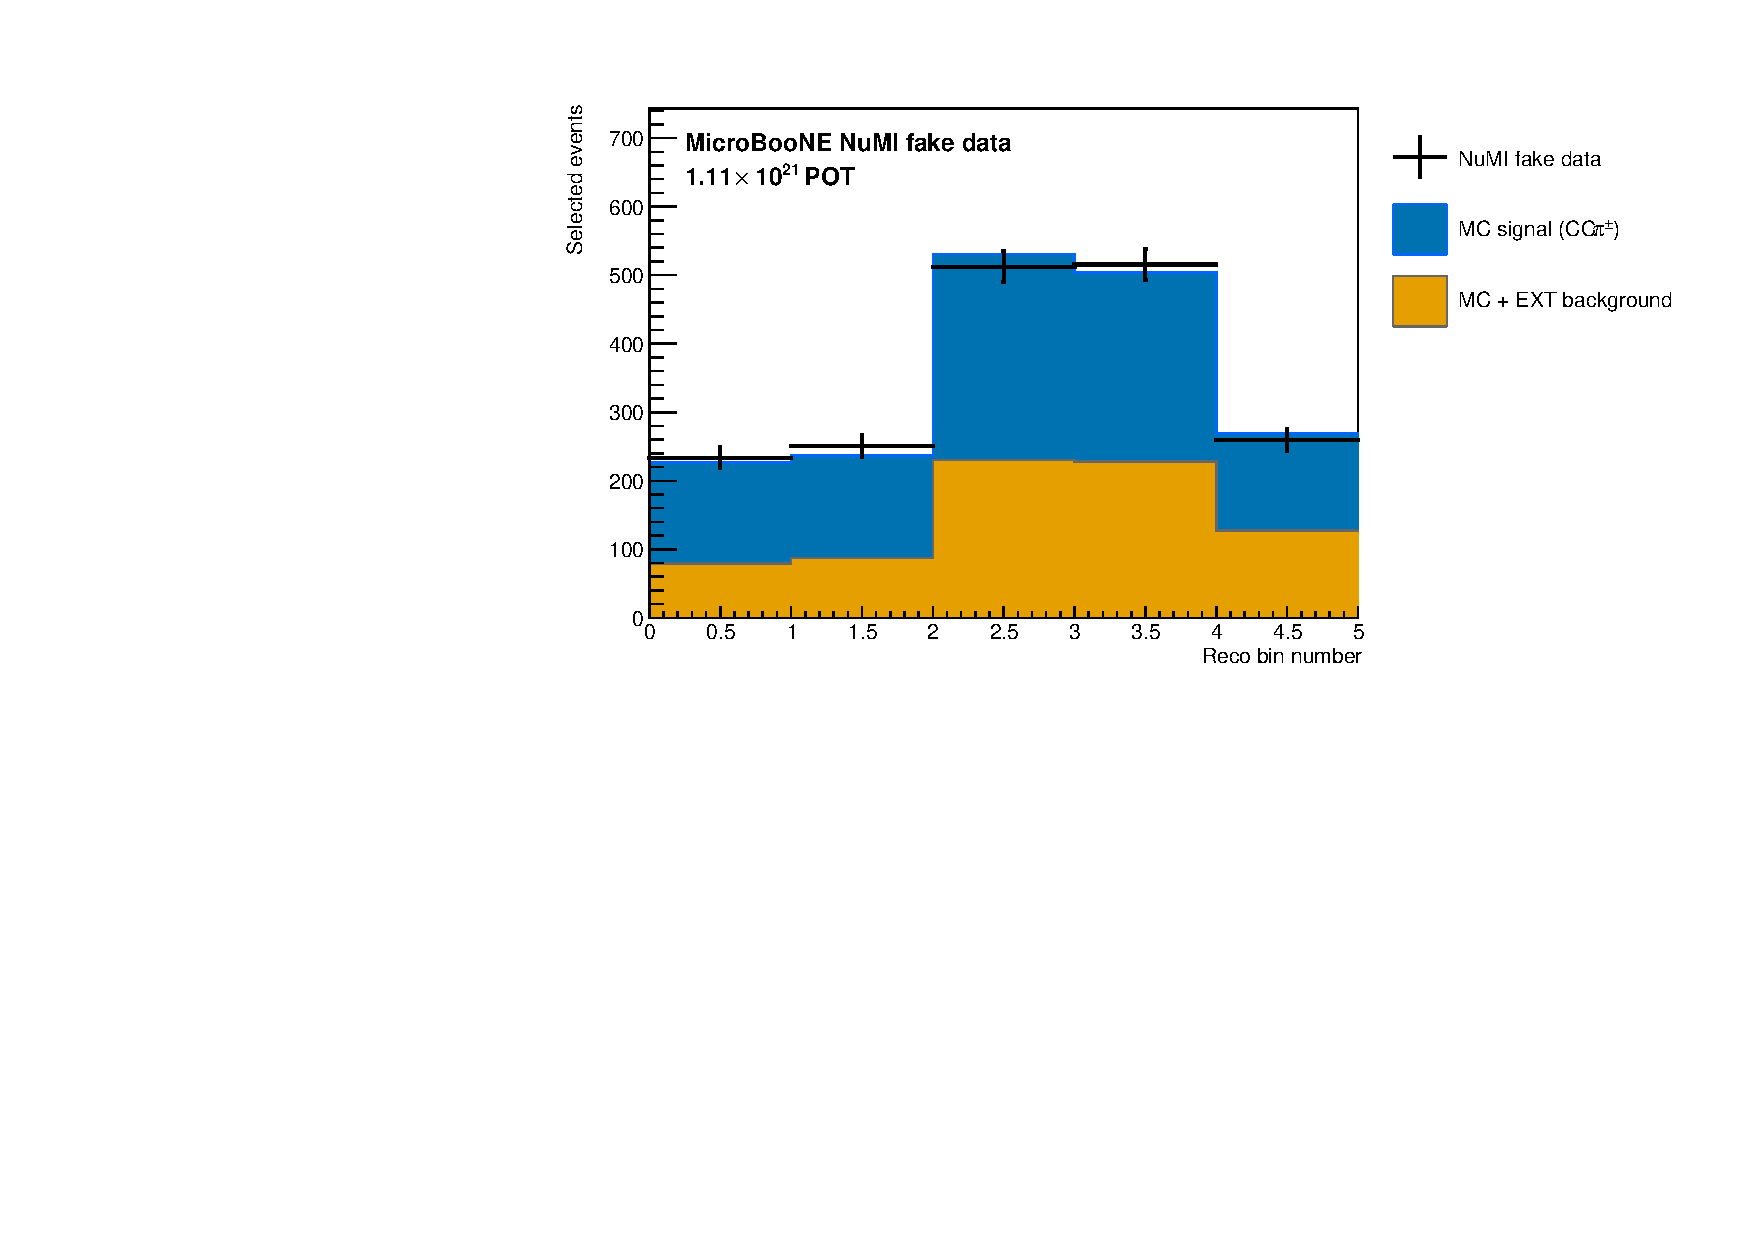
\includegraphics[width=\textwidth]{fw_reco_rhc_thmupi}\caption{$\theta_{\mu\pi}$}\end{subfigure}\hfill
  \begin{subfigure}[b]{0.32\textwidth}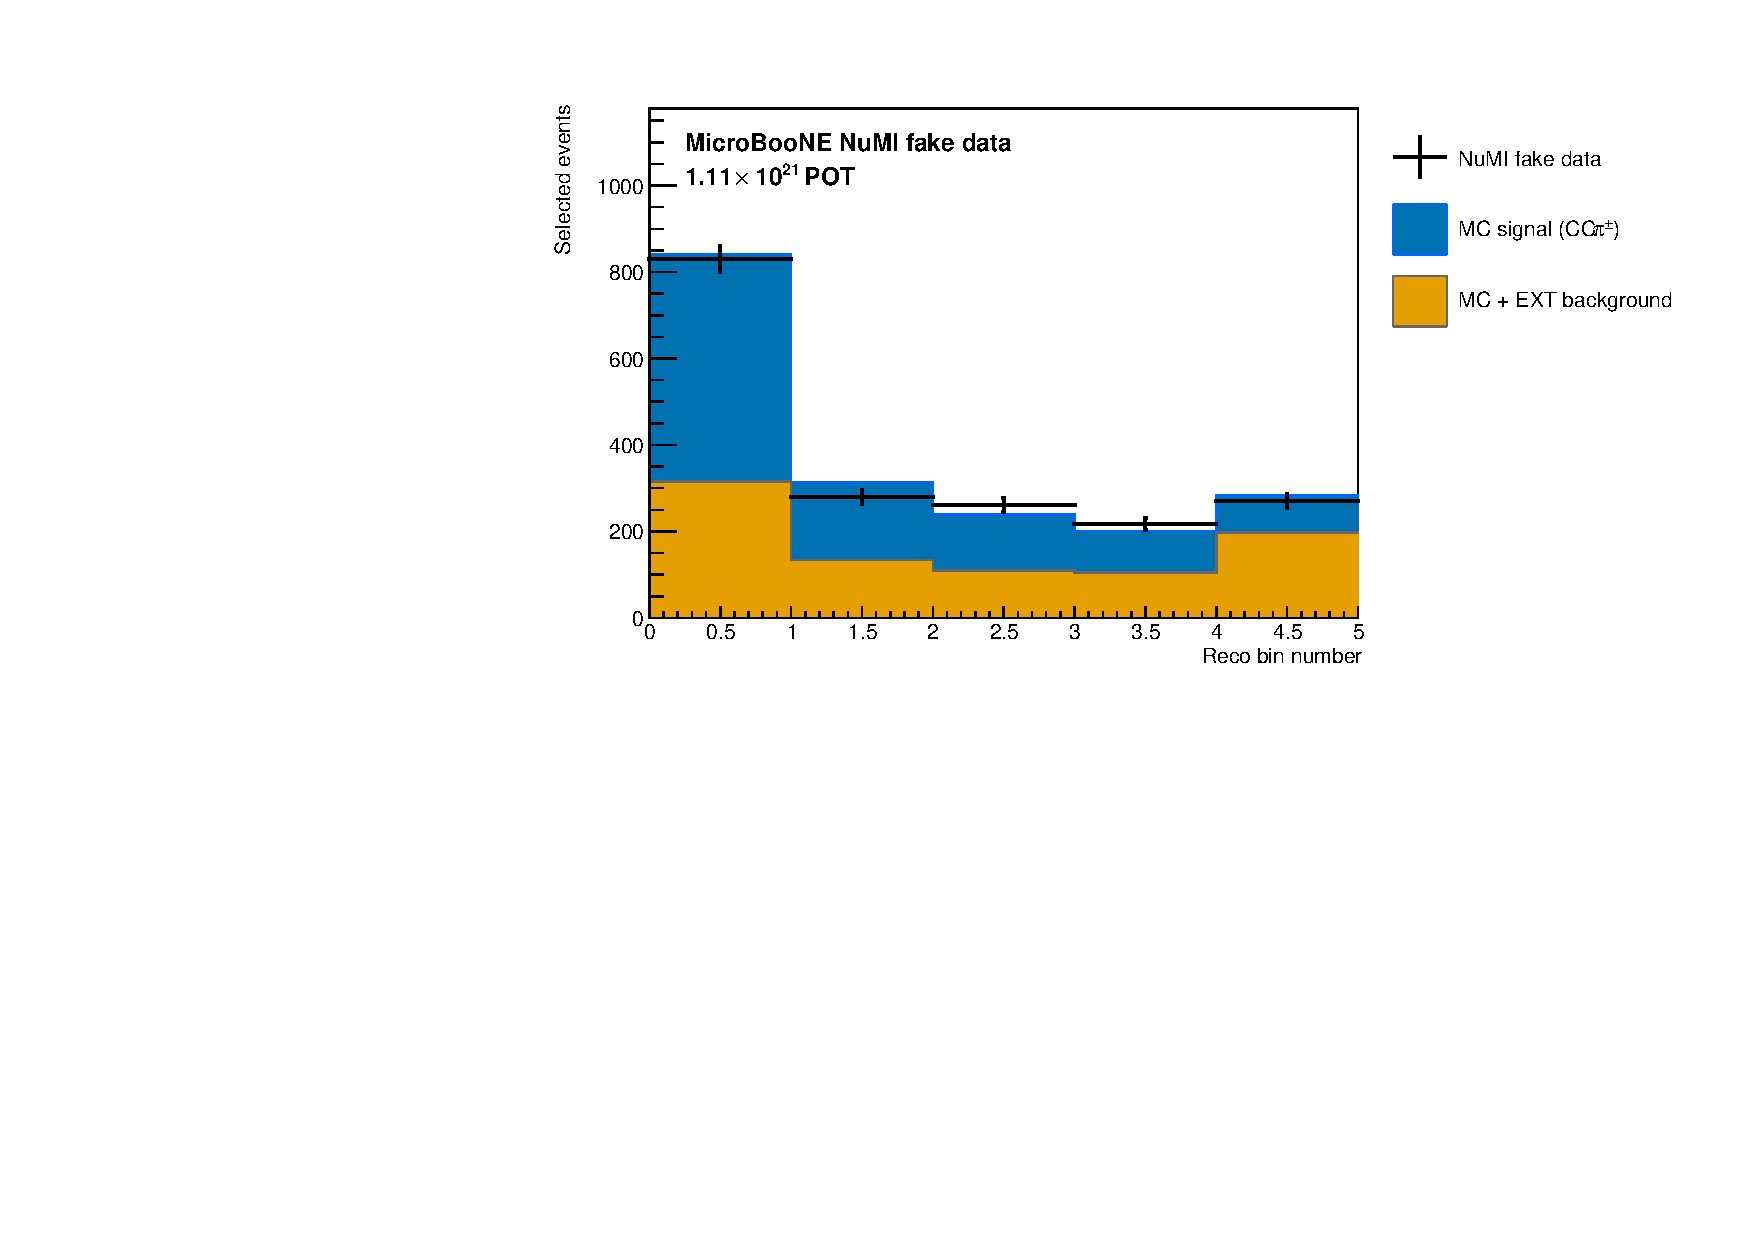
\includegraphics[width=\textwidth]{fw_reco_rhc_thetamu}\caption{$\theta_\mu$}\end{subfigure}
  \caption{Reconstructed-space spectra, RHC full exposure (Runs~1$+$2$+$3$+$4a$+$4b$+$4c);
    same components as Fig.~\ref{fig:reco_spectra}.}
  \label{fig:reco_spectra_rhc}
\end{figure}

\begin{figure}[H]
  \centering
  \begin{subfigure}[b]{0.32\textwidth}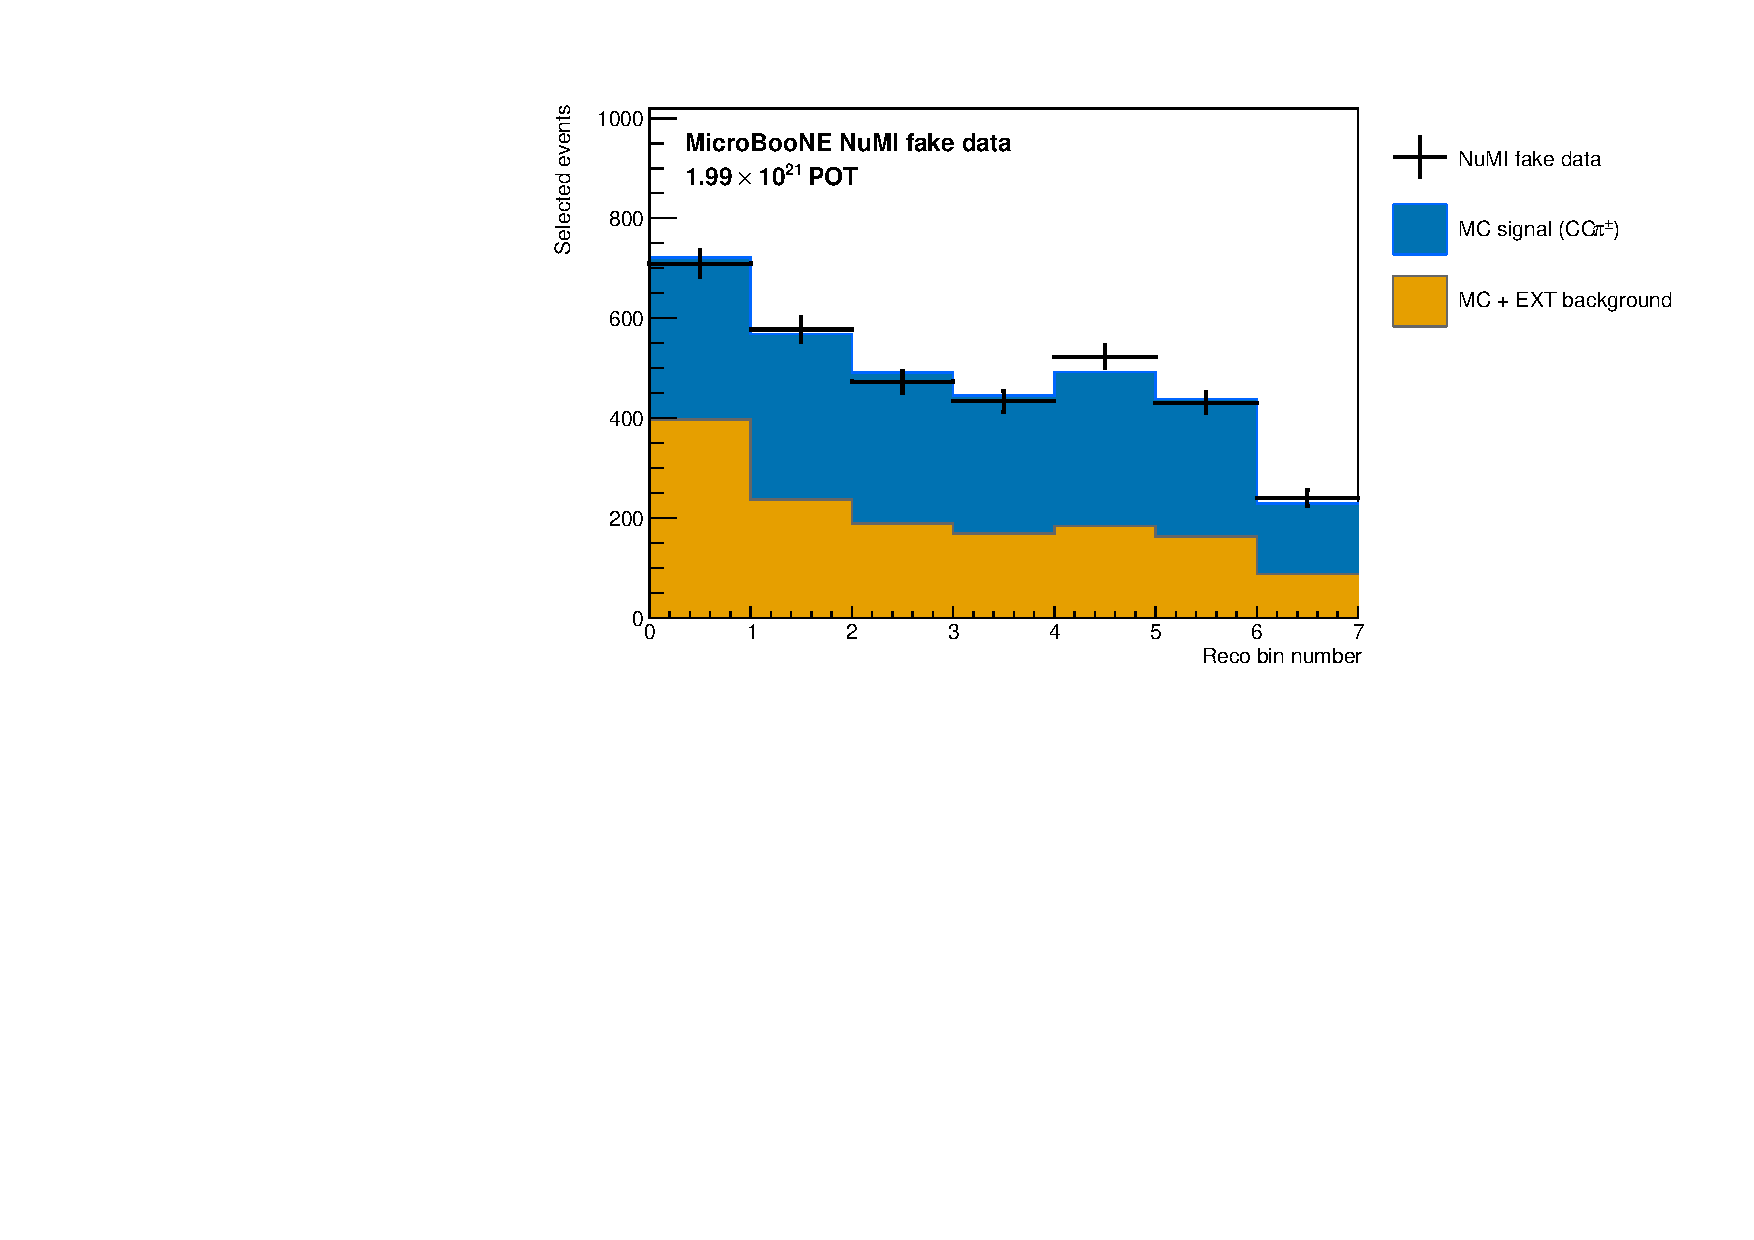
\includegraphics[width=\textwidth]{fw_reco_comb_pmu}\caption{$p_\mu$}\end{subfigure}\hfill
  \begin{subfigure}[b]{0.32\textwidth}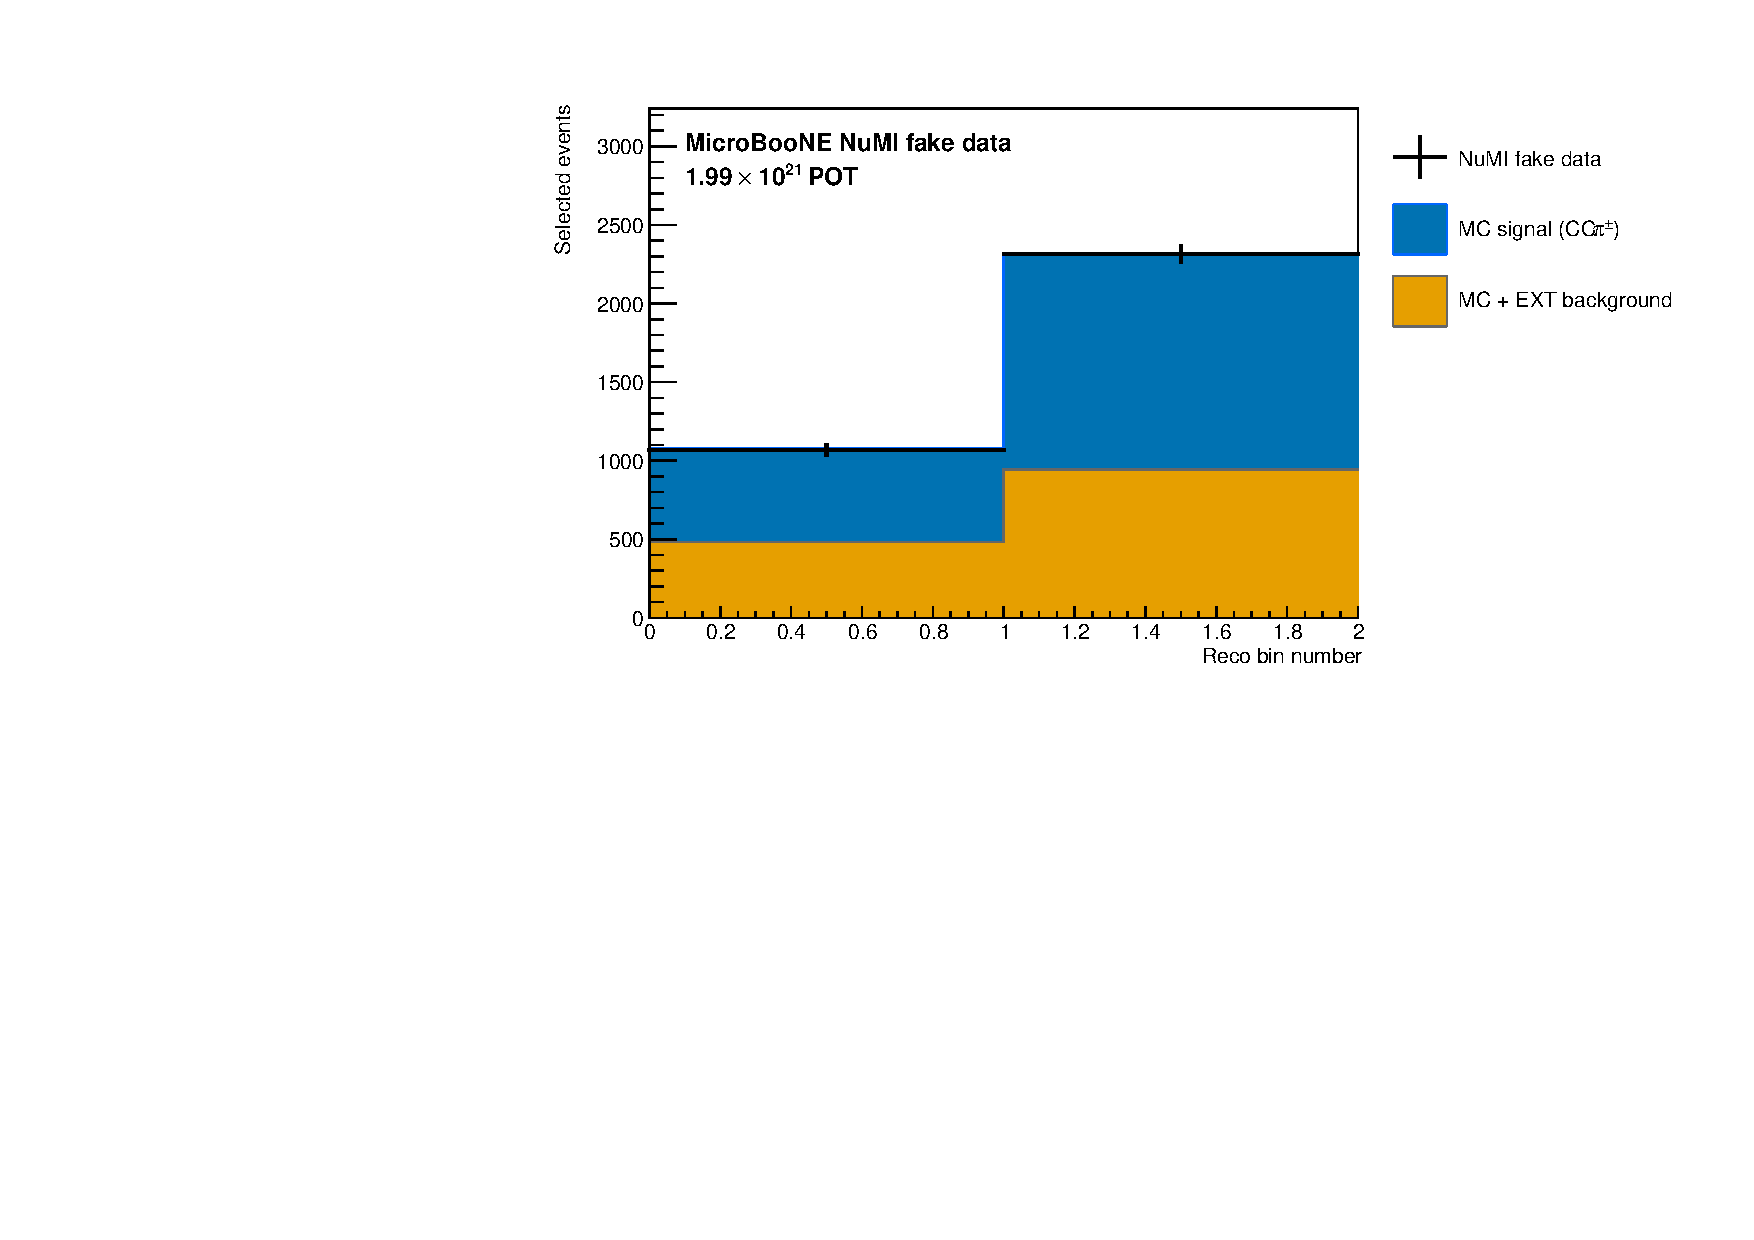
\includegraphics[width=\textwidth]{fw_reco_comb_ppi}\caption{$p_\pi$}\end{subfigure}\hfill
  \begin{subfigure}[b]{0.32\textwidth}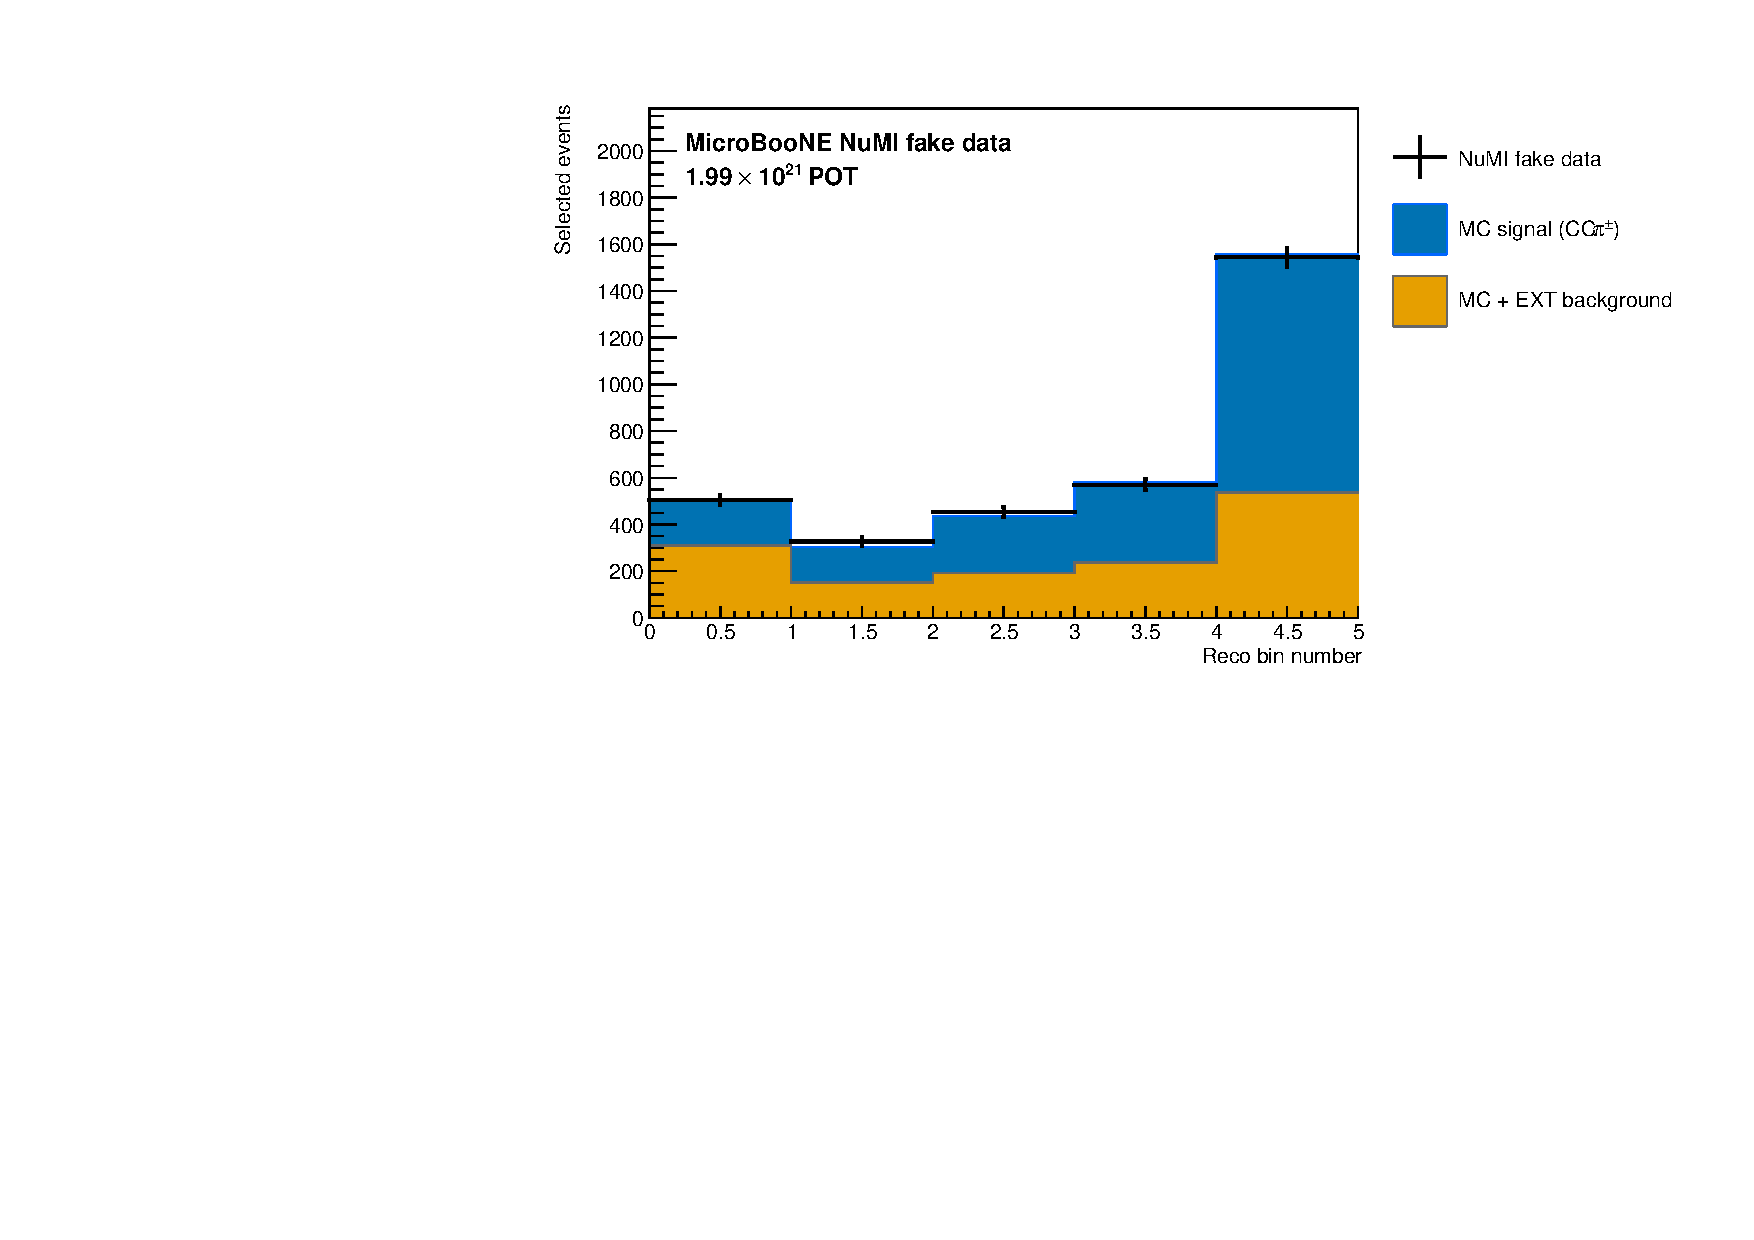
\includegraphics[width=\textwidth]{fw_reco_comb_costhmu}\caption{$\cos\theta_\mu$}\end{subfigure}\\[6pt]
  \begin{subfigure}[b]{0.32\textwidth}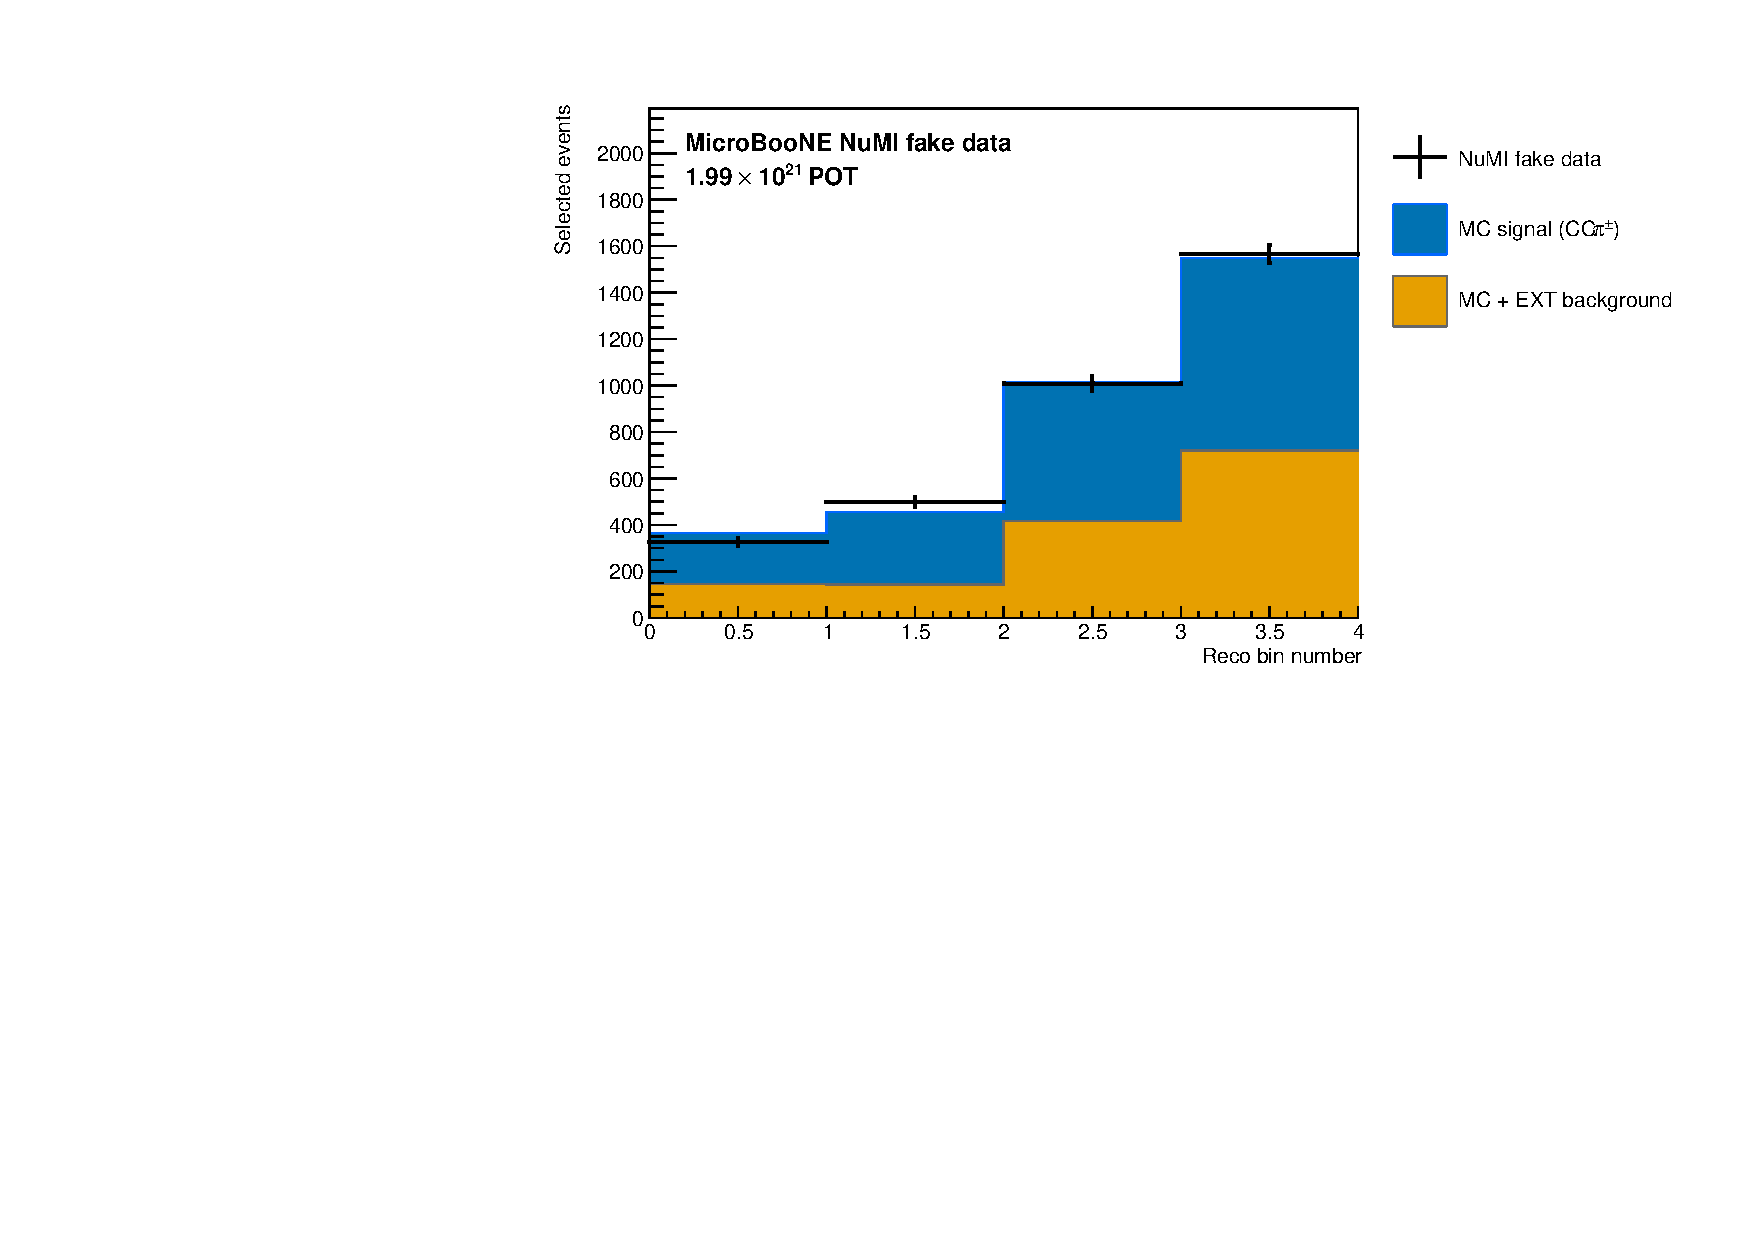
\includegraphics[width=\textwidth]{fw_reco_comb_costhpi}\caption{$\cos\theta_\pi$}\end{subfigure}\hfill
  \begin{subfigure}[b]{0.32\textwidth}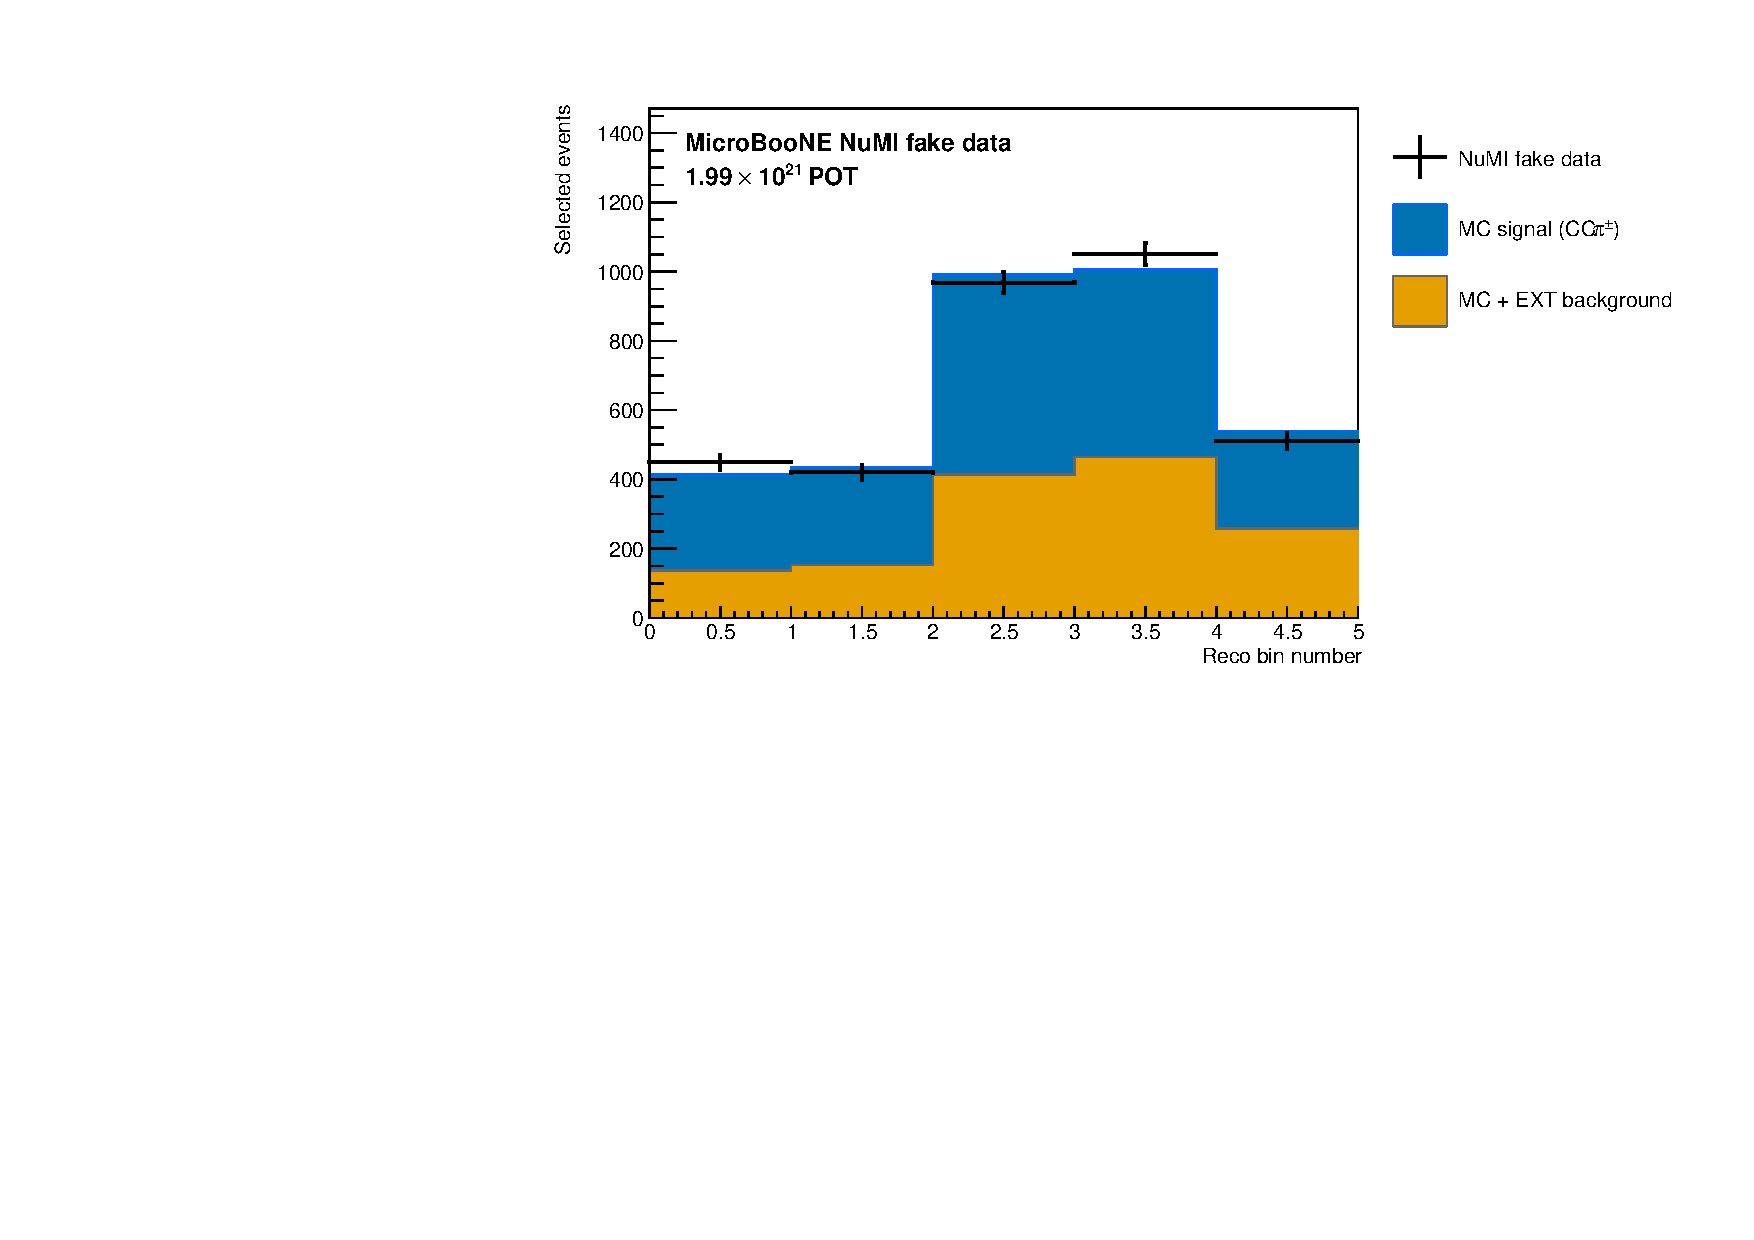
\includegraphics[width=\textwidth]{fw_reco_comb_thmupi}\caption{$\theta_{\mu\pi}$}\end{subfigure}\hfill
  \begin{subfigure}[b]{0.32\textwidth}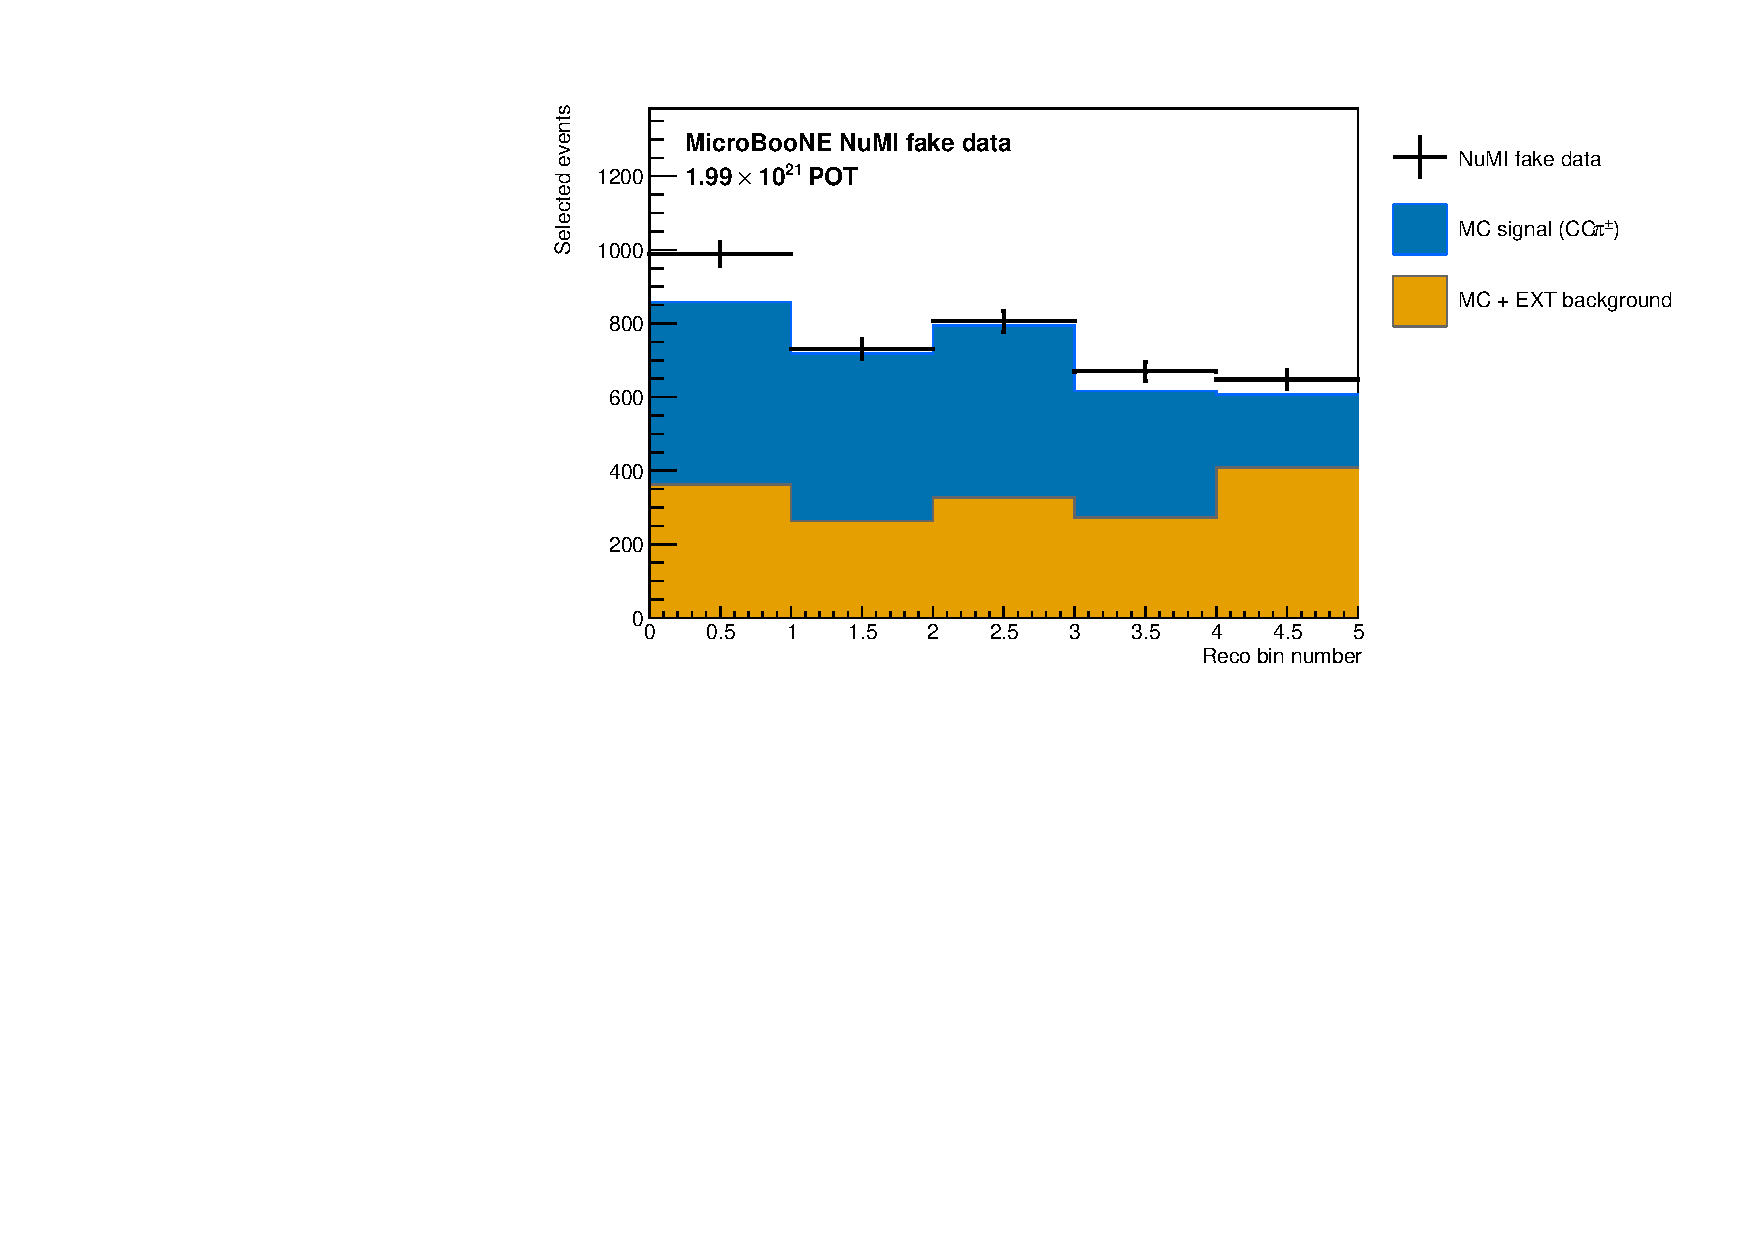
\includegraphics[width=\textwidth]{fw_reco_comb_thetamu}\caption{$\theta_\mu$}\end{subfigure}
  \caption{Reconstructed-space spectra, combined FHC$+$RHC (per-mode normalised);
    same components as Fig.~\ref{fig:reco_spectra}.}
  \label{fig:reco_spectra_comb}
\end{figure}

Figure~\ref{fig:response} shows the smearceptance matrices $S$ (\S\ref{sec:unfolding_resp};
colour scale includes the efficiency, so the columns sum to $\varepsilon_j$, not to unity)
for the six observables at the released binning. The column-normalised diagonals of the
released FHC responses are
$0.86$--$0.95$ for the best-resolved bin of each angular observable (the forward bin of
$\cos\theta_\mu$, the first bin of the others), $0.67$--$0.88$ elsewhere in
$\cos\theta_\mu$, $\theta_\mu$, $\cos\theta_\pi$ and $\theta_{\mu\pi}$, and
$0.81$, $0.65$, $0.57$, $0.50$, $0.45$, $0.38$, $0.33$ for the seven $p_\mu$ bins: $p_\mu$
is \emph{not} near-diagonal, because its bins ($0.2$--$0.5$~GeV/$c$ wide) are narrower
than the $30\%$ resolution of the MCS estimator, which reconstructs $63\%$ of the
selected sample and is intrinsically less precise than range. The $0.68$ diagonal
criterion quoted for $p_\pi$ below is therefore not a criterion this analysis applies
uniformly: for $p_\mu$ the Wiener-SVD regularisation absorbs the migration (the released
$A_C$ row sums stay at $0.66$--$0.91$, \S\ref{sec:ac_rowsums}) and the closure and
ensemble tests pass, whereas for $p_\pi$ the migration is accompanied by a physical
saturation of the estimator, which no regularisation recovers. A finer $p_\mu$ binning is
excluded by the same resolution (\suppref{Sec.}{sec:binopt}).

\emph{$p_\pi$.} At any fine binning the $p_\pi$ response is strongly non-diagonal, because
the range estimator saturates near $0.34\GeVc$ once pions interact hadronically before
stopping; that is a physical limit rather than an algorithmic one, and the fine-bin study
is in the technical supplement (\suppref{Sec.}{sec:ppi_bias}). The adopted two-bin
response shown here is sufficiently diagonal, with column-normalised diagonals of $91\%$
and $76\%$, but it carries only threshold-versus-above-threshold information: the upper
bin is an inclusive region, not a resolved spectral point (\S\ref{sec:status_matrix}).

\begin{figure}[H]
  \centering
  \begin{subfigure}[b]{0.32\textwidth}
    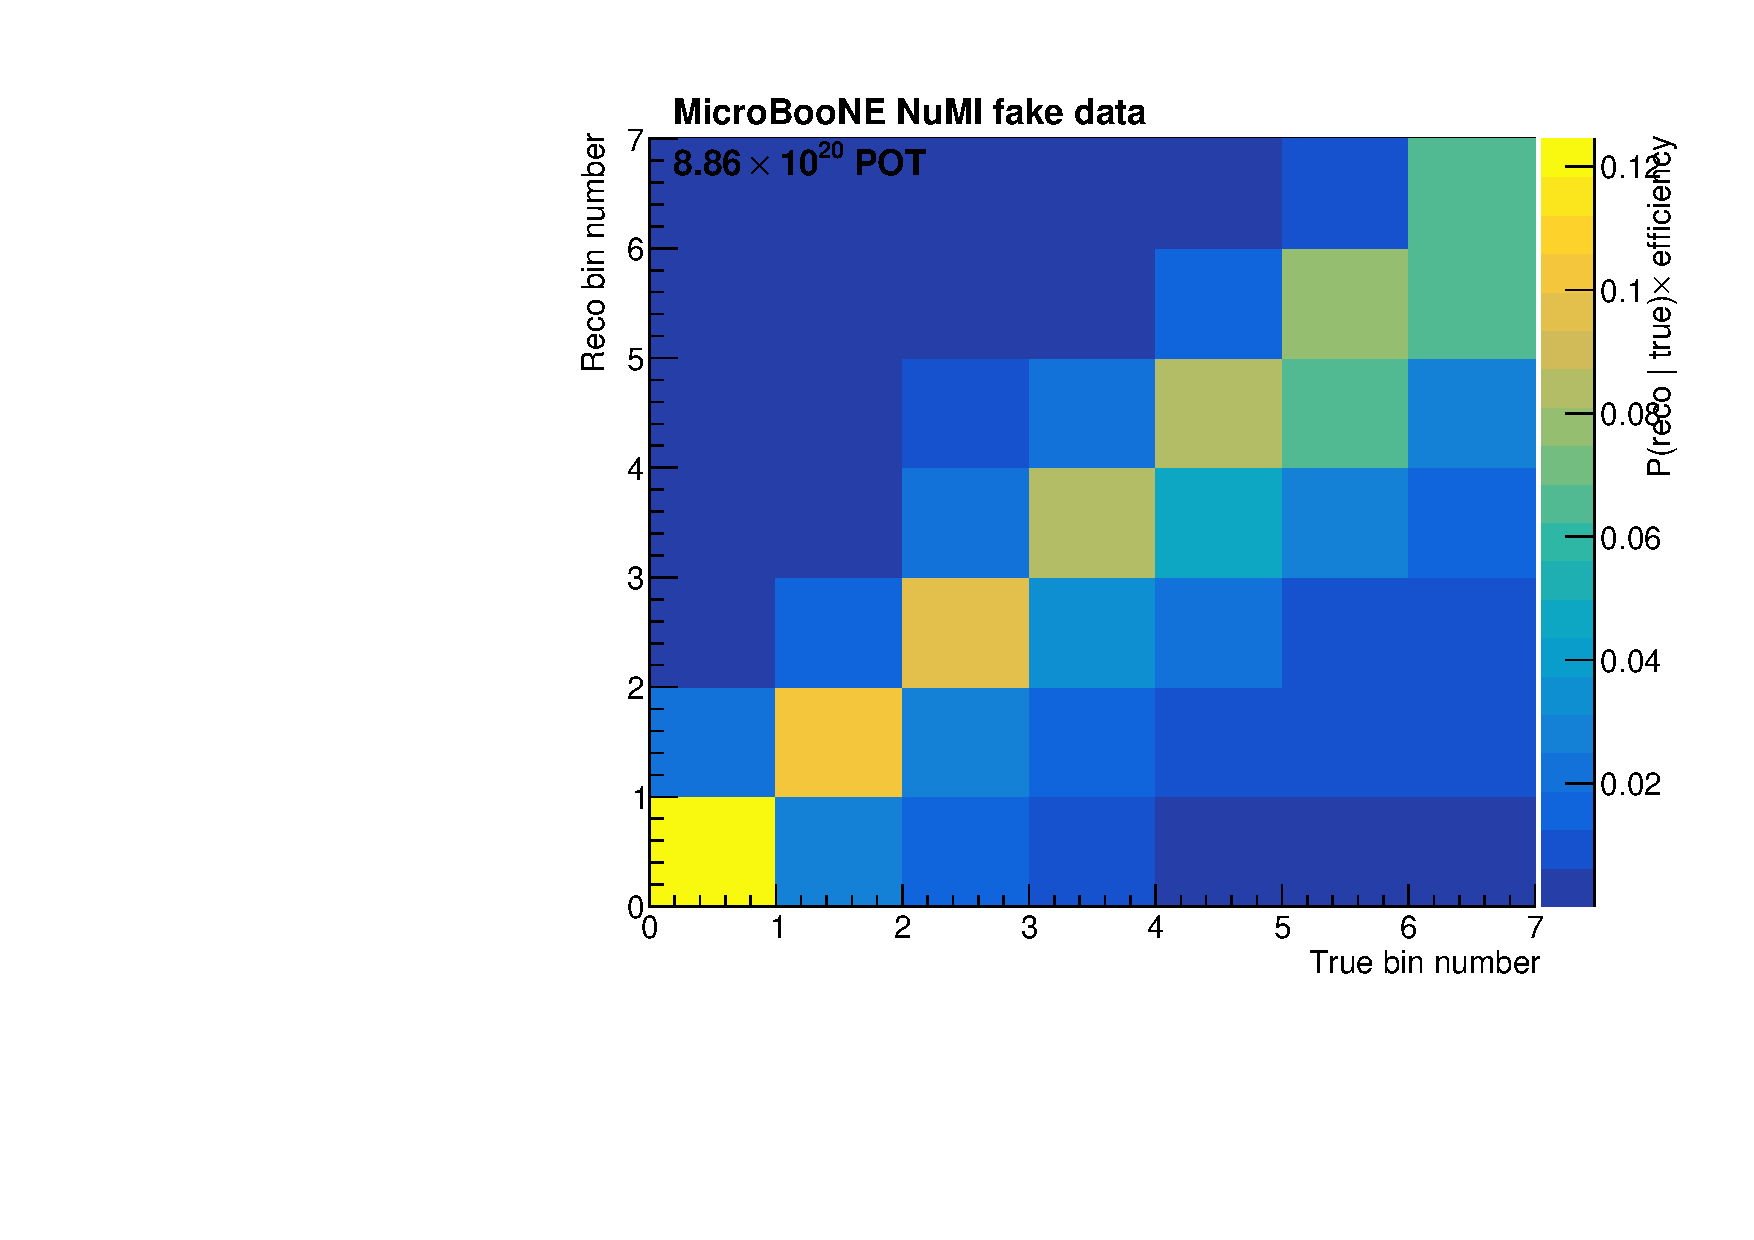
\includegraphics[width=\textwidth]{fw_resp_pmu}
    \caption{$p_\mu$}
  \end{subfigure}
  \hfill
  \begin{subfigure}[b]{0.32\textwidth}
    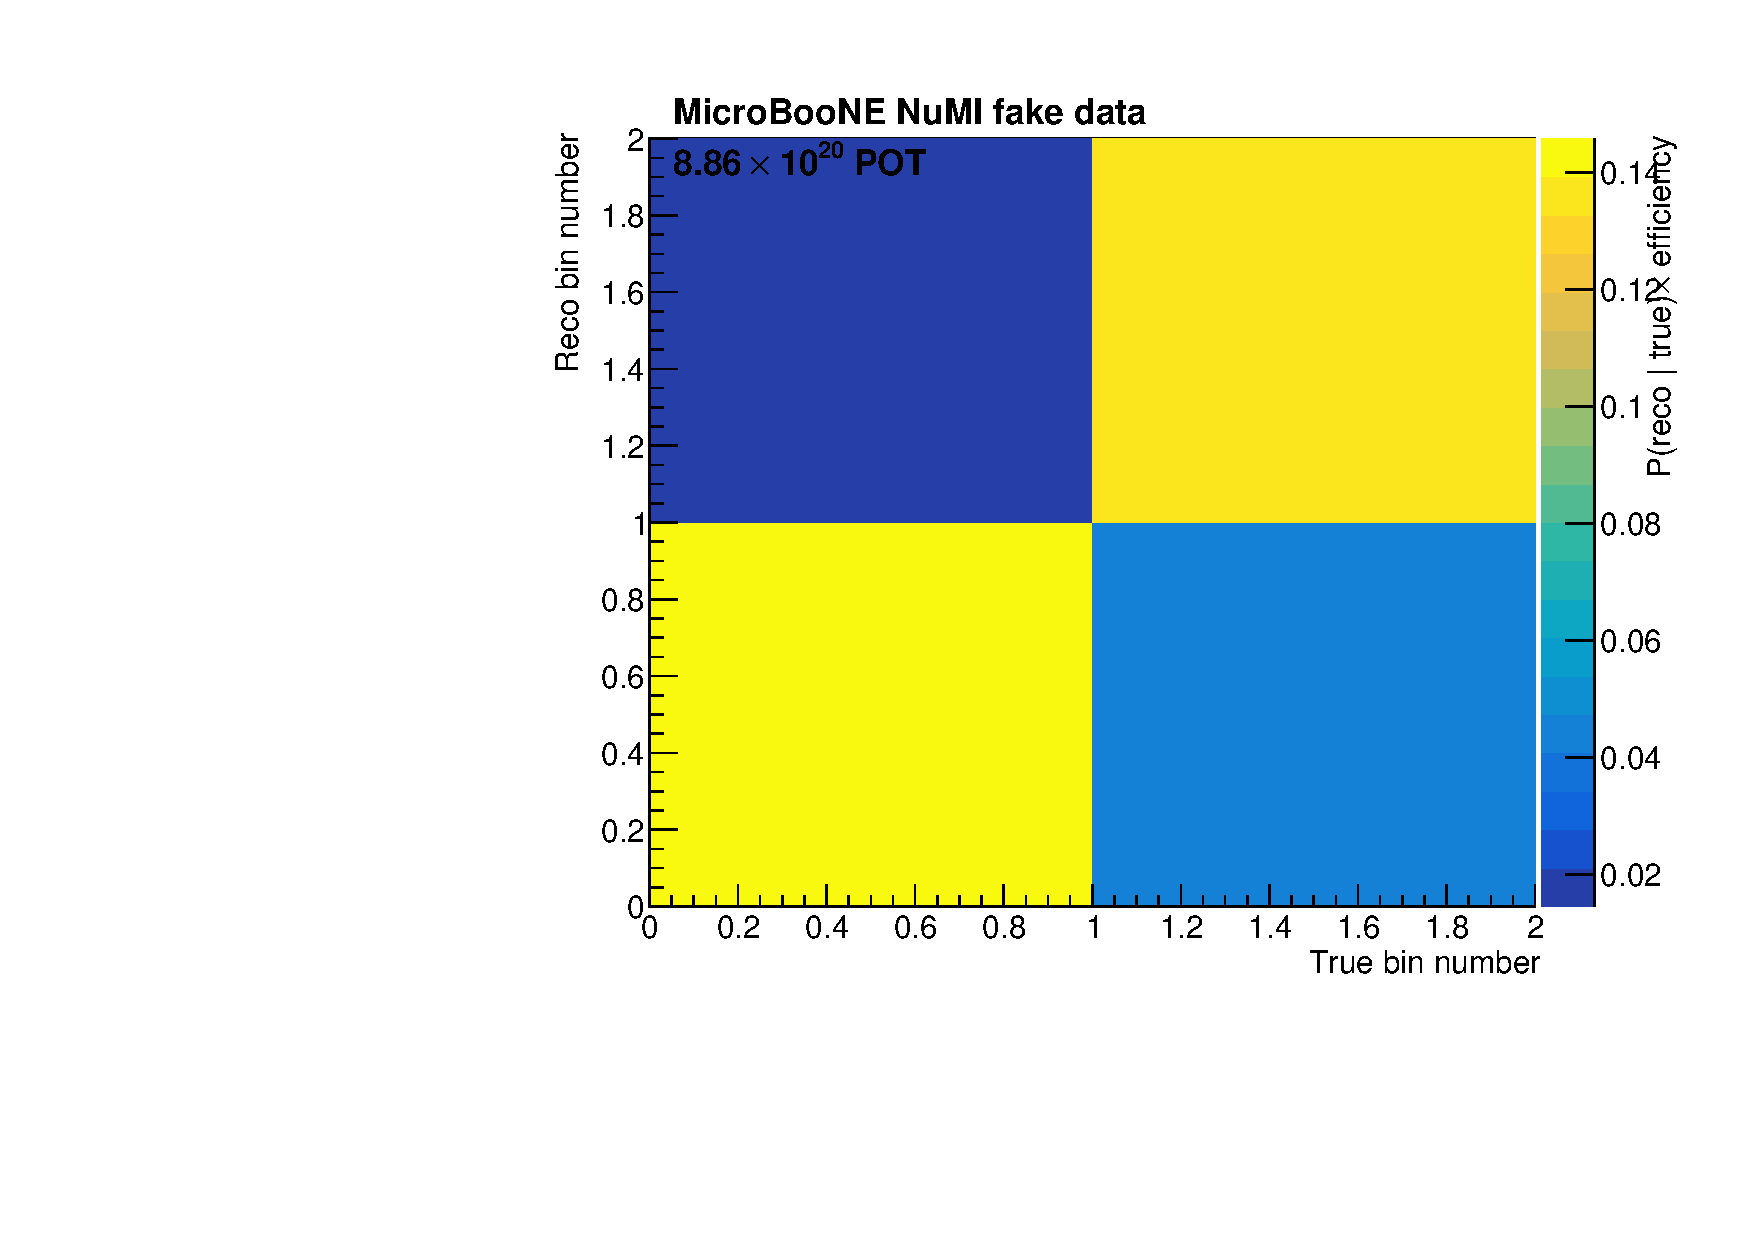
\includegraphics[width=\textwidth]{fw_resp_ppi2bin}
    \caption{$p_\pi$}
  \end{subfigure}
  \hfill
  \begin{subfigure}[b]{0.32\textwidth}
    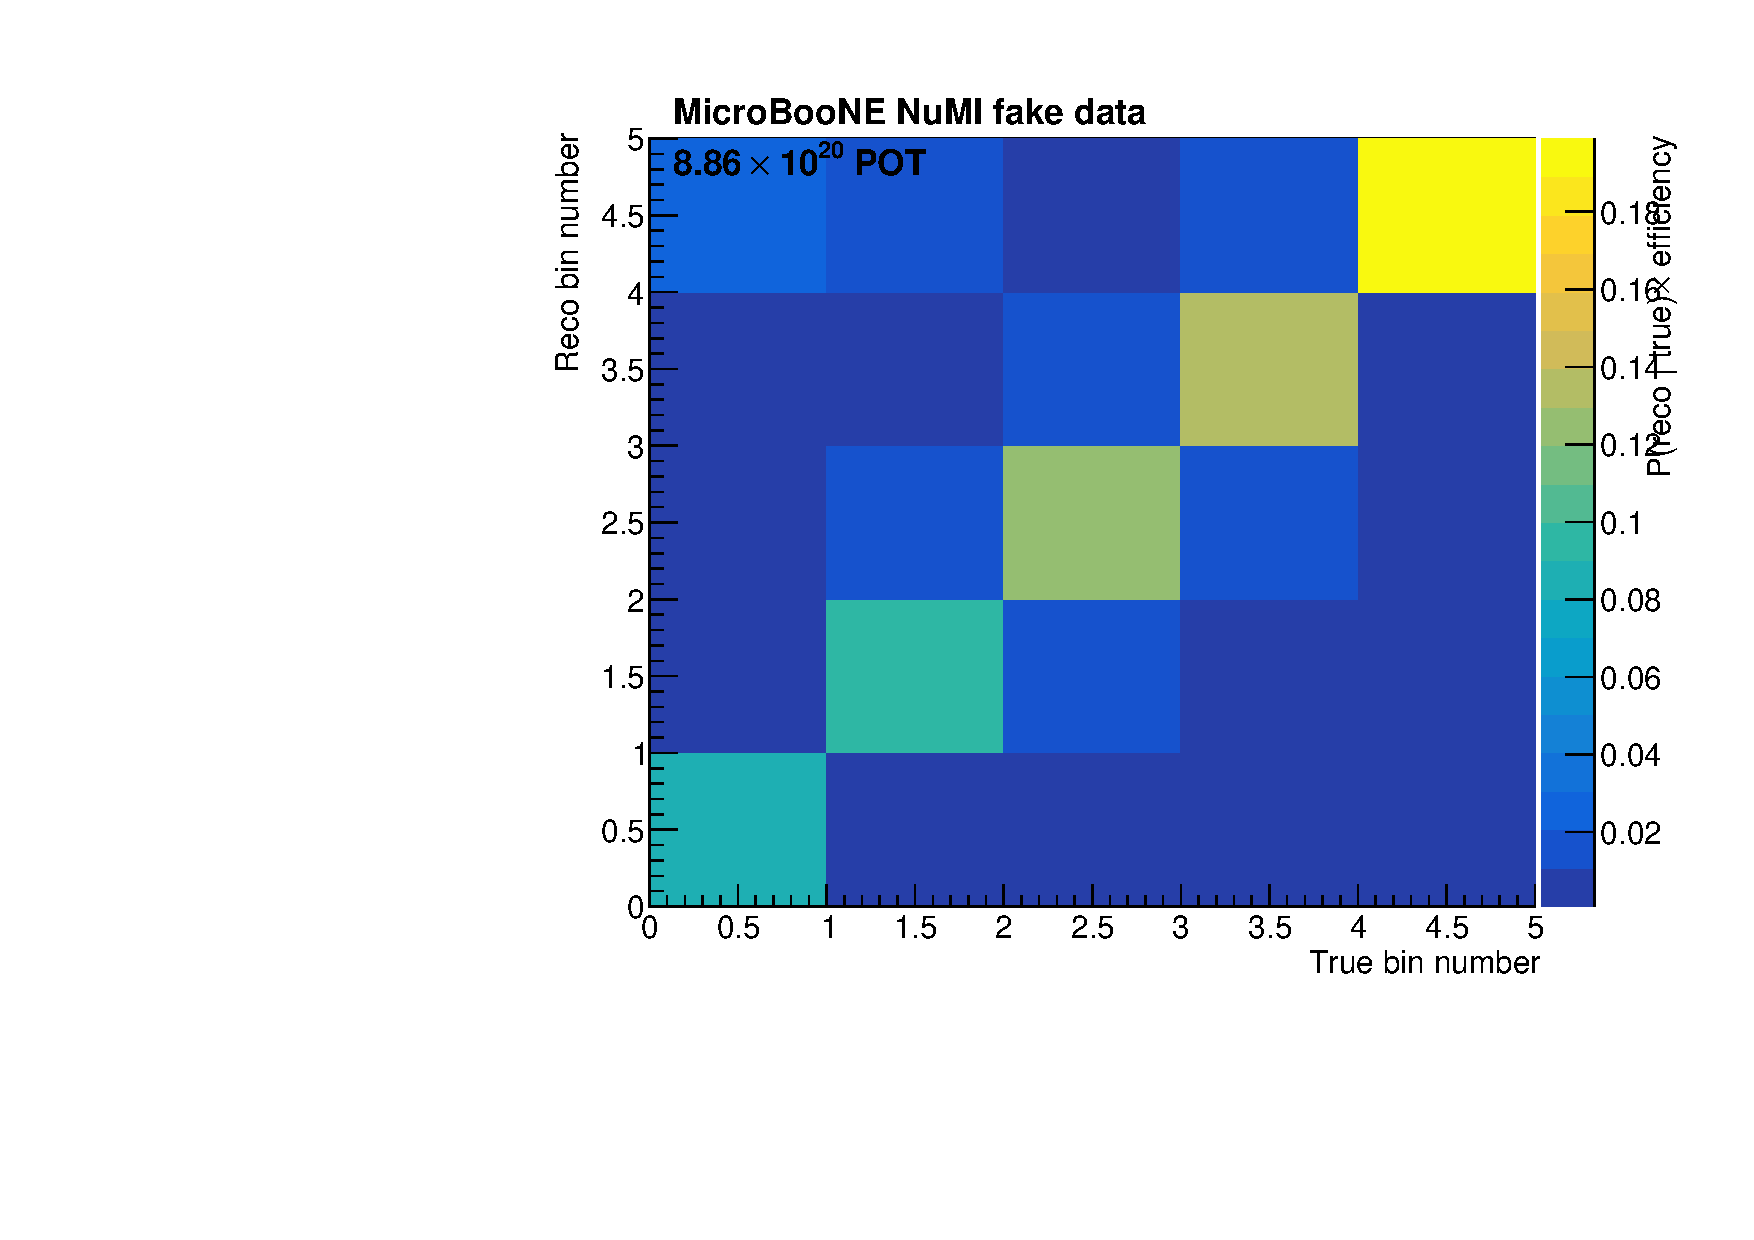
\includegraphics[width=\textwidth]{fw_resp_costhmu}
    \caption{$\cos\theta_\mu$}
  \end{subfigure}\\[6pt]
  \begin{subfigure}[b]{0.32\textwidth}
    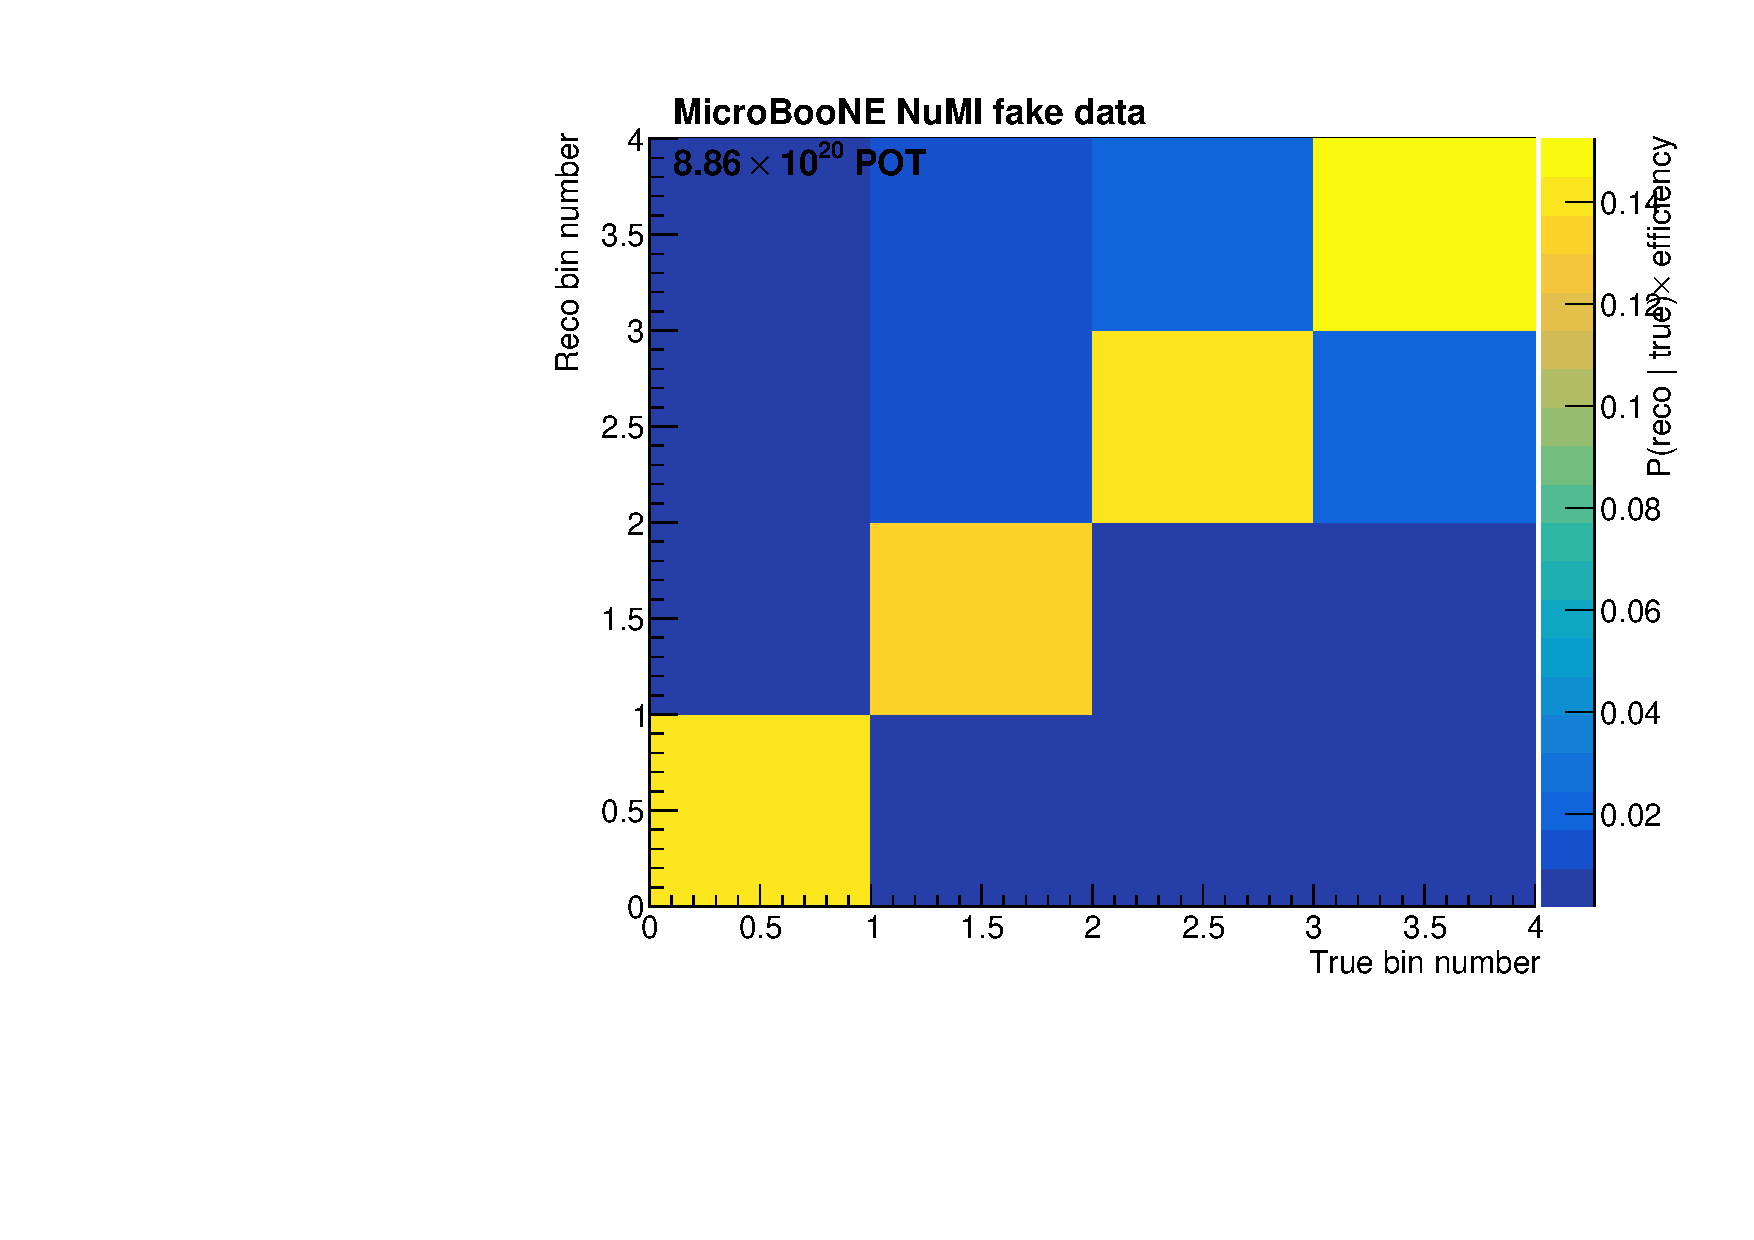
\includegraphics[width=\textwidth]{fw_resp_costhpi}
    \caption{$\cos\theta_\pi$}
  \end{subfigure}
  \hfill
  \begin{subfigure}[b]{0.32\textwidth}
    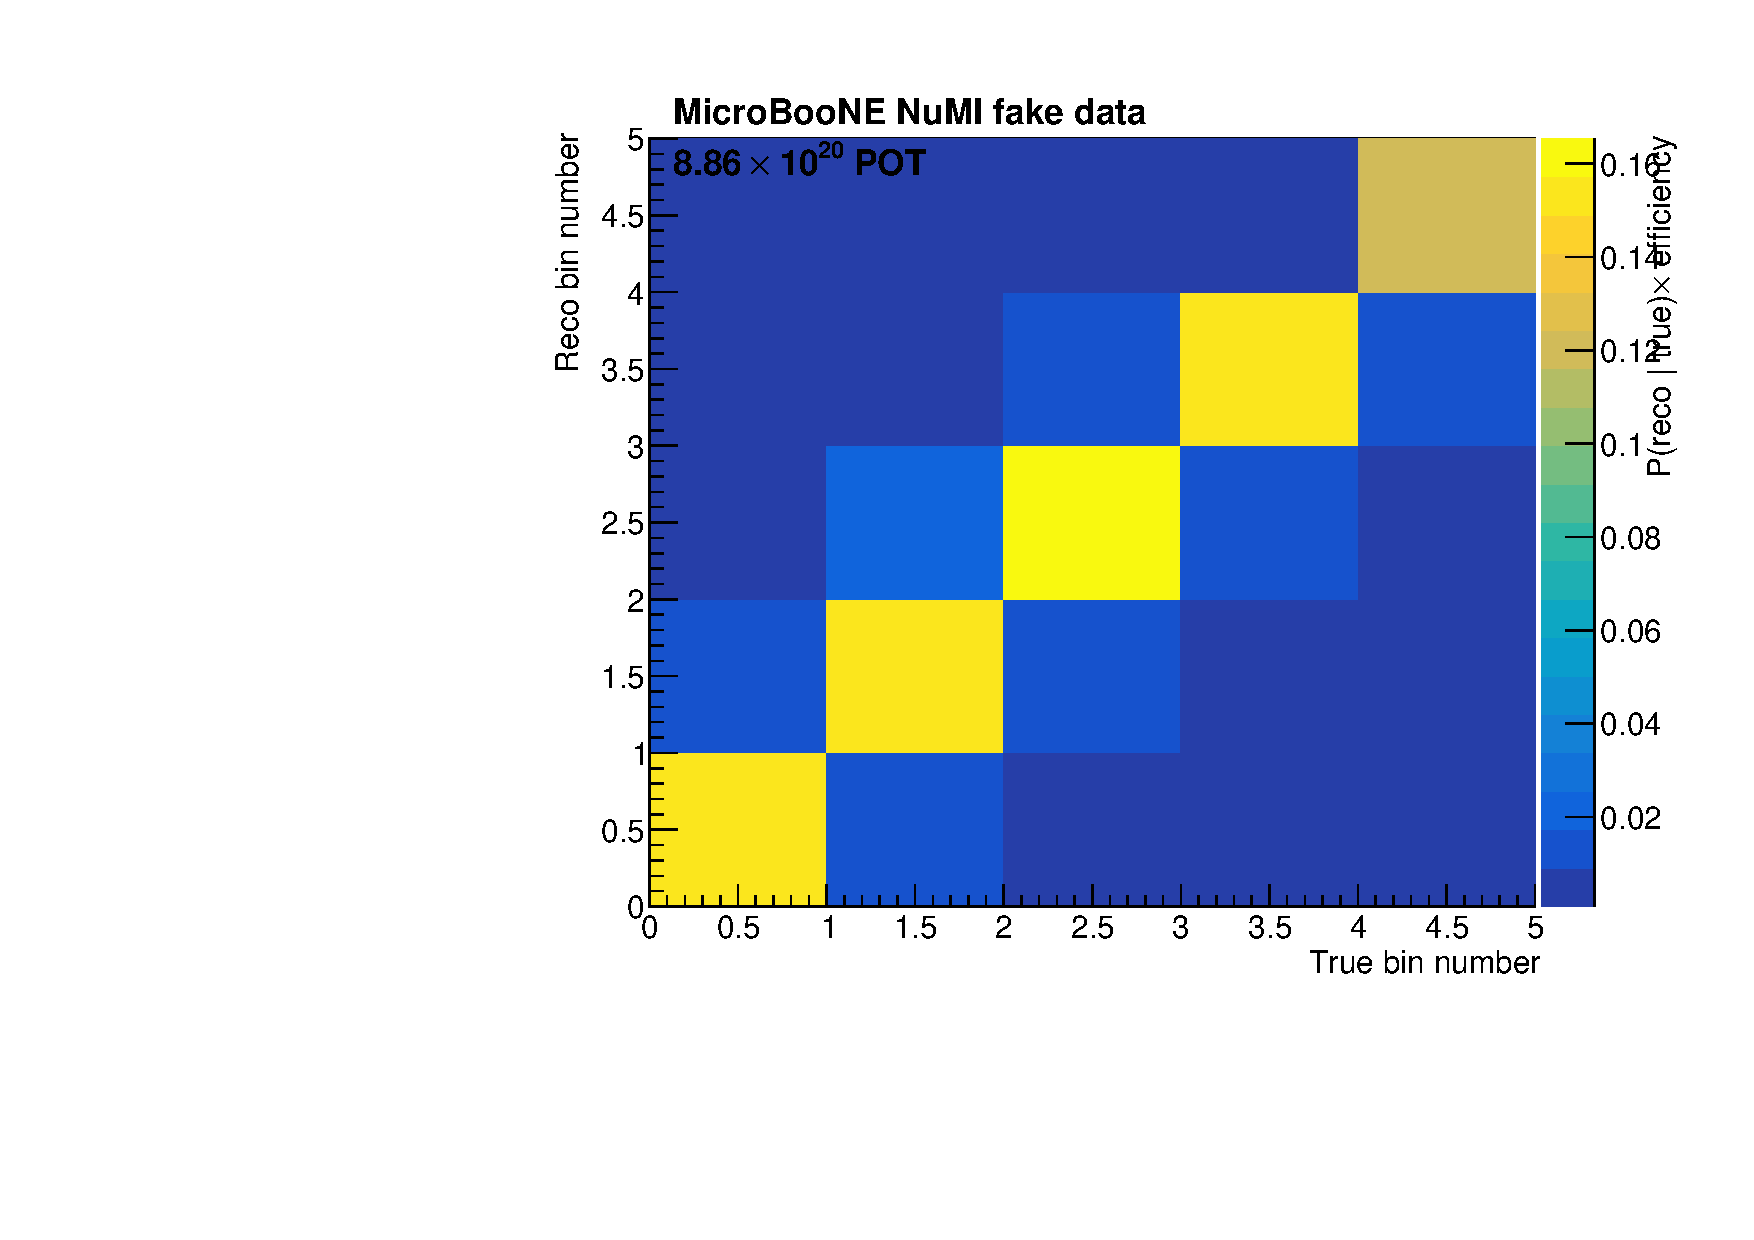
\includegraphics[width=\textwidth]{fw_resp_thmupi}
    \caption{$\theta_{\mu\pi}$}
  \end{subfigure}
  \hfill
  \begin{subfigure}[b]{0.32\textwidth}
    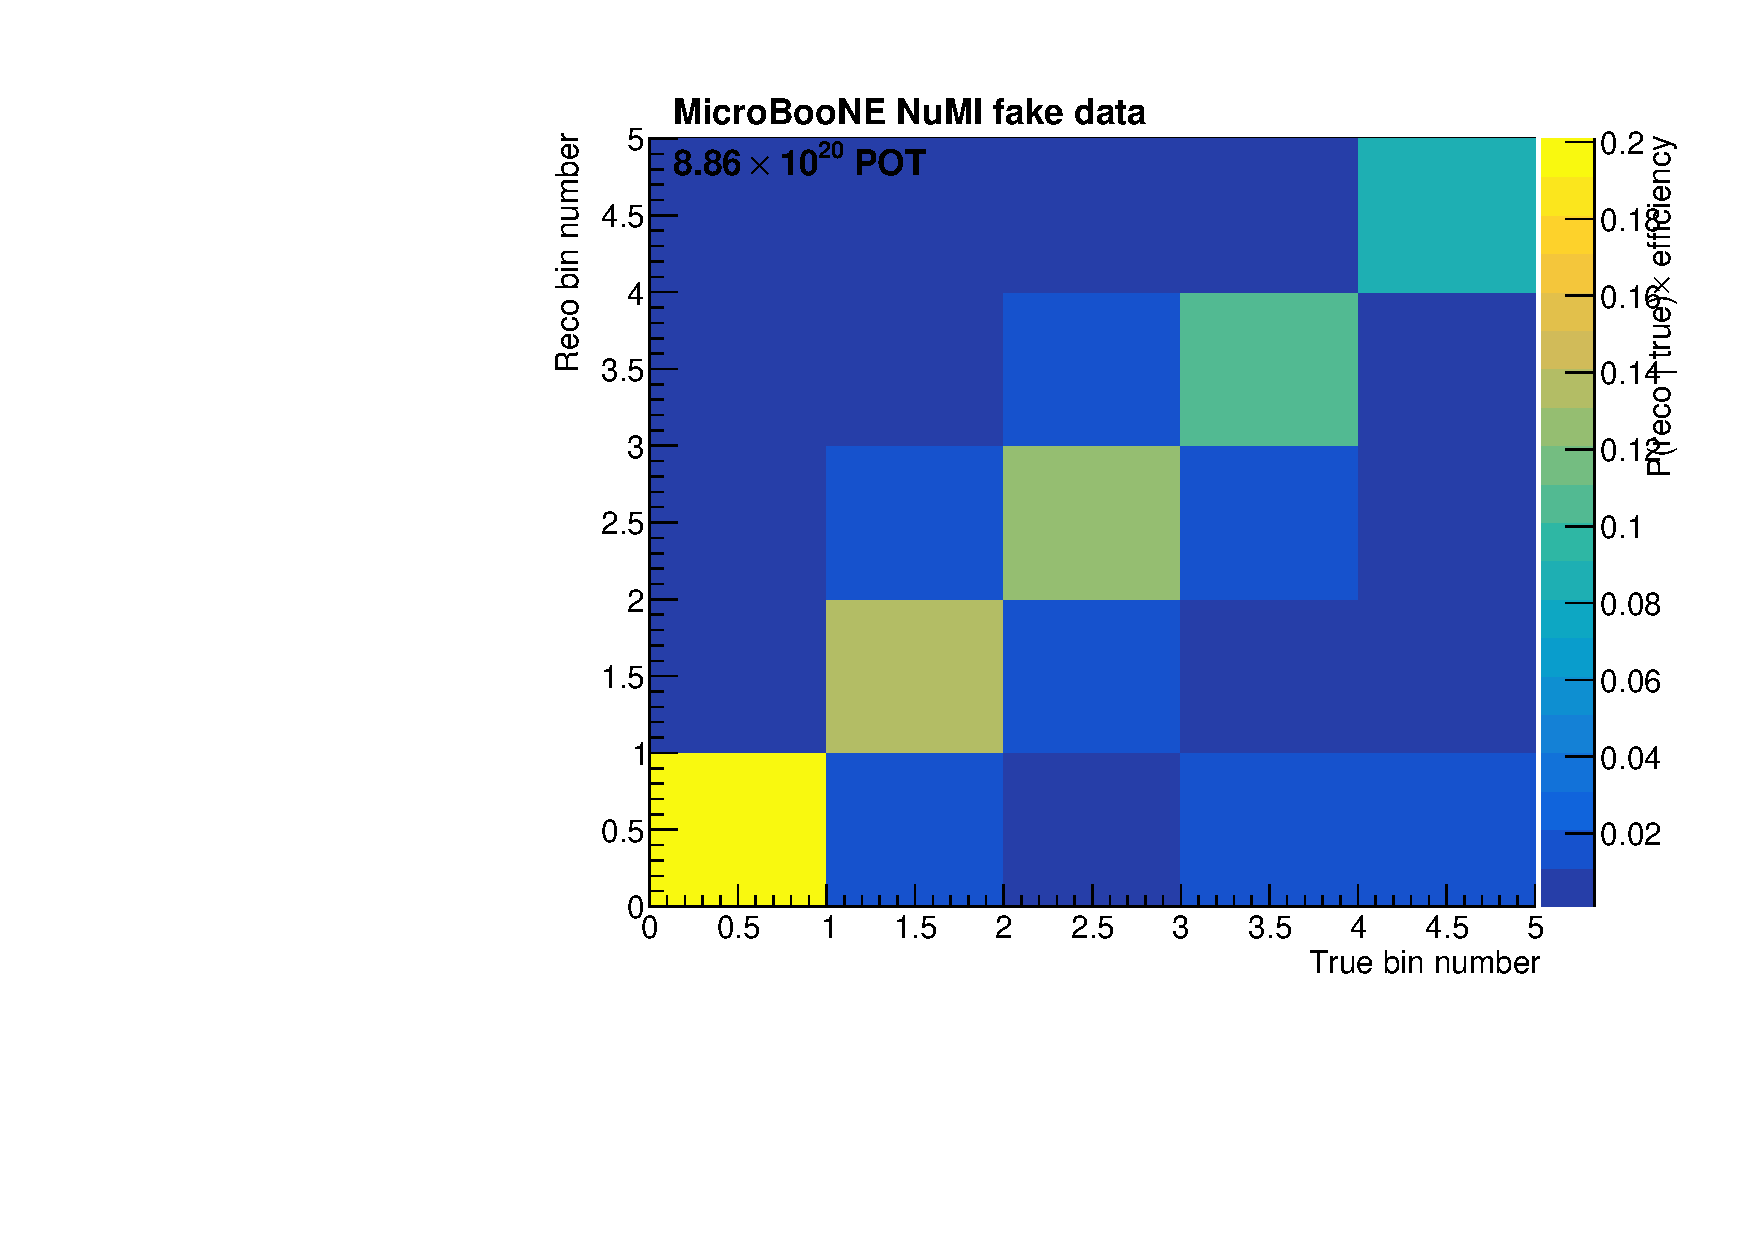
\includegraphics[width=\textwidth]{fw_resp_thetamu}
    \caption{$\theta_\mu$}
  \end{subfigure}
  \caption{Smearceptance matrices $S_{ij}=\varepsilon_j M_{ij}$, FHC, exactly as passed to
    the unfolder. Five panels are at the released
    binning, including the released two-bin $p_\pi$ response ($91\%$ and $76\%$ column-normalised
    diagonals); the rejected five-bin $p_\pi$ response, which shows the reconstructed events
    piling into the lowest bin from every true bin, is \suppref{Fig.}{fig:resp_ppi5}.}
  \label{fig:response}
\end{figure}

Figure~\ref{fig:efficiency} shows the selection efficiency per true bin for
all six observables, computed as the ratio of selected to generated signal MC.

\begin{figure}[H]
  \centering
  \begin{subfigure}[b]{0.32\textwidth}
    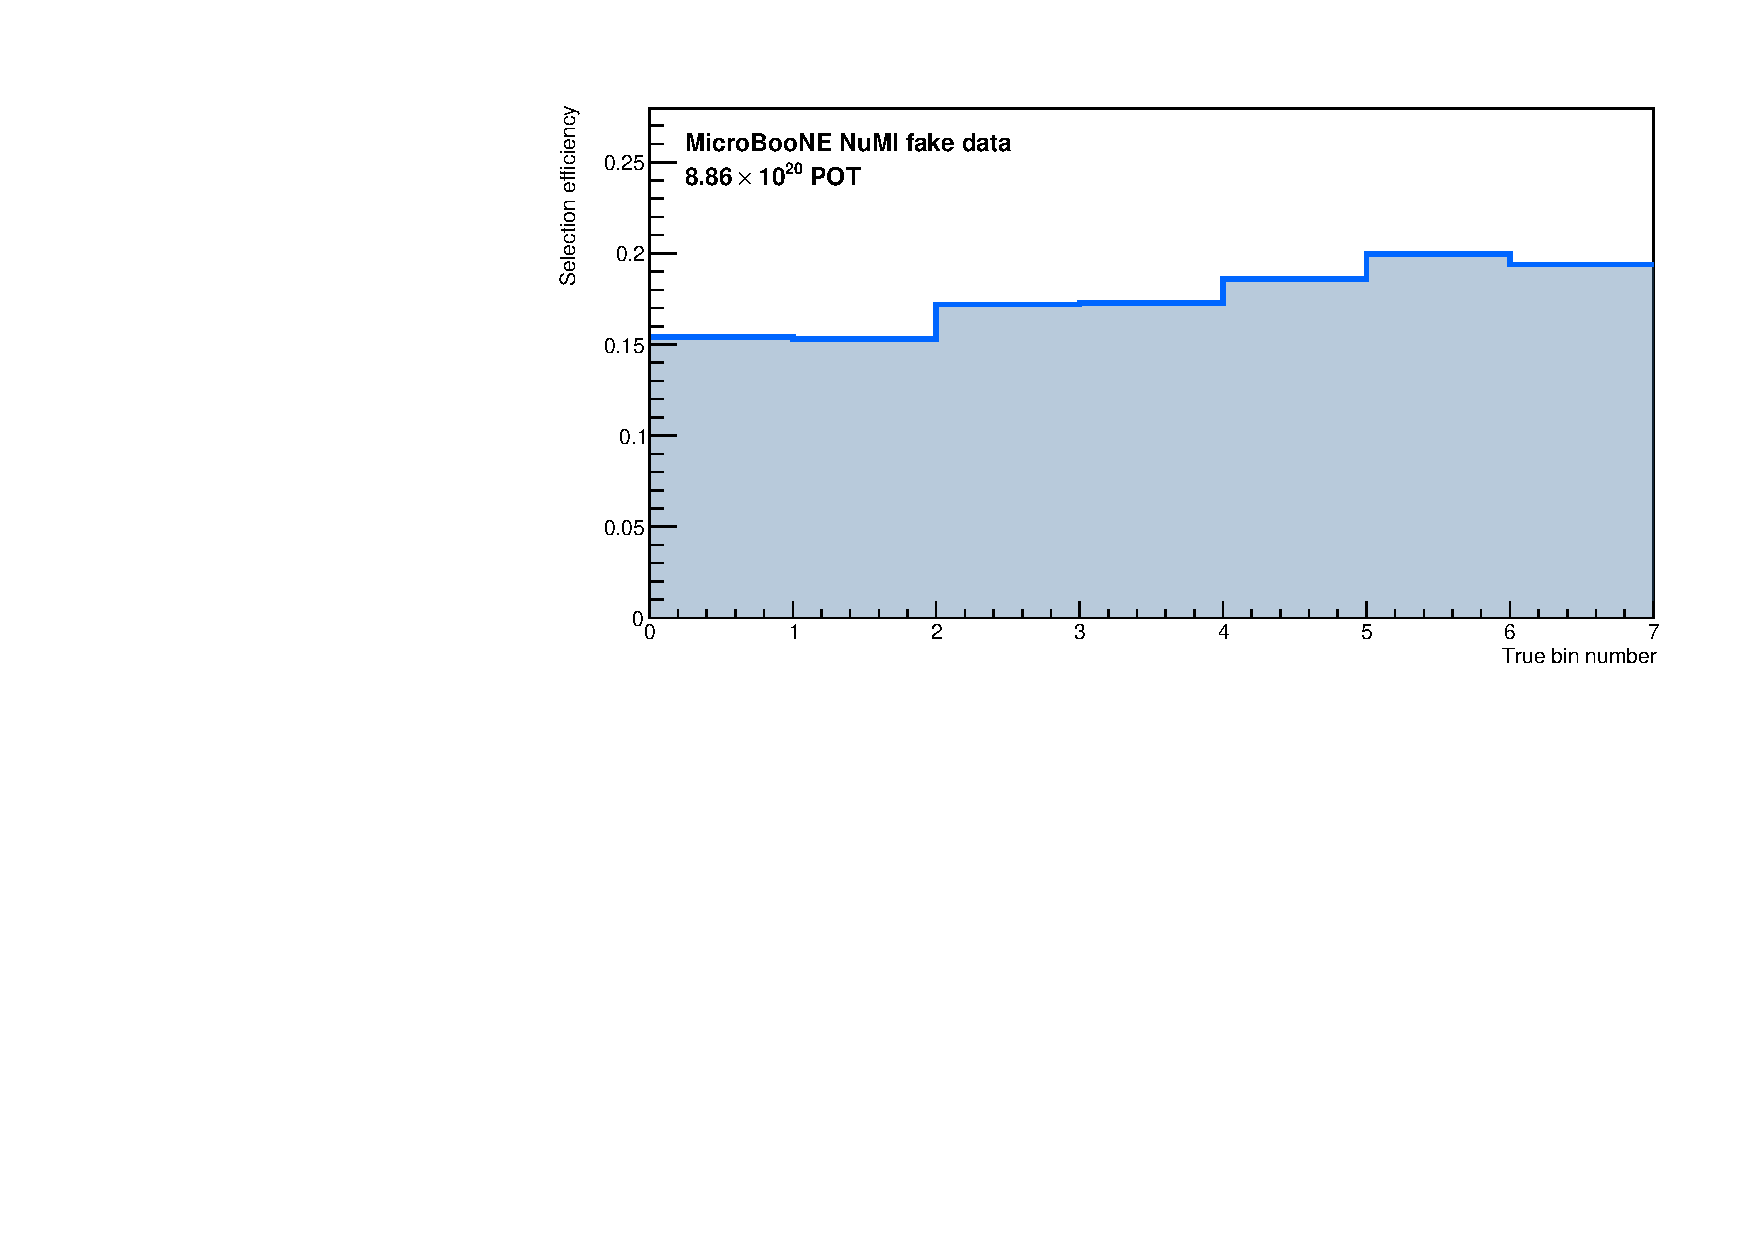
\includegraphics[width=\textwidth]{fw_eff_pmu}
    \caption{$p_\mu$}
  \end{subfigure}
  \hfill
  \begin{subfigure}[b]{0.32\textwidth}
    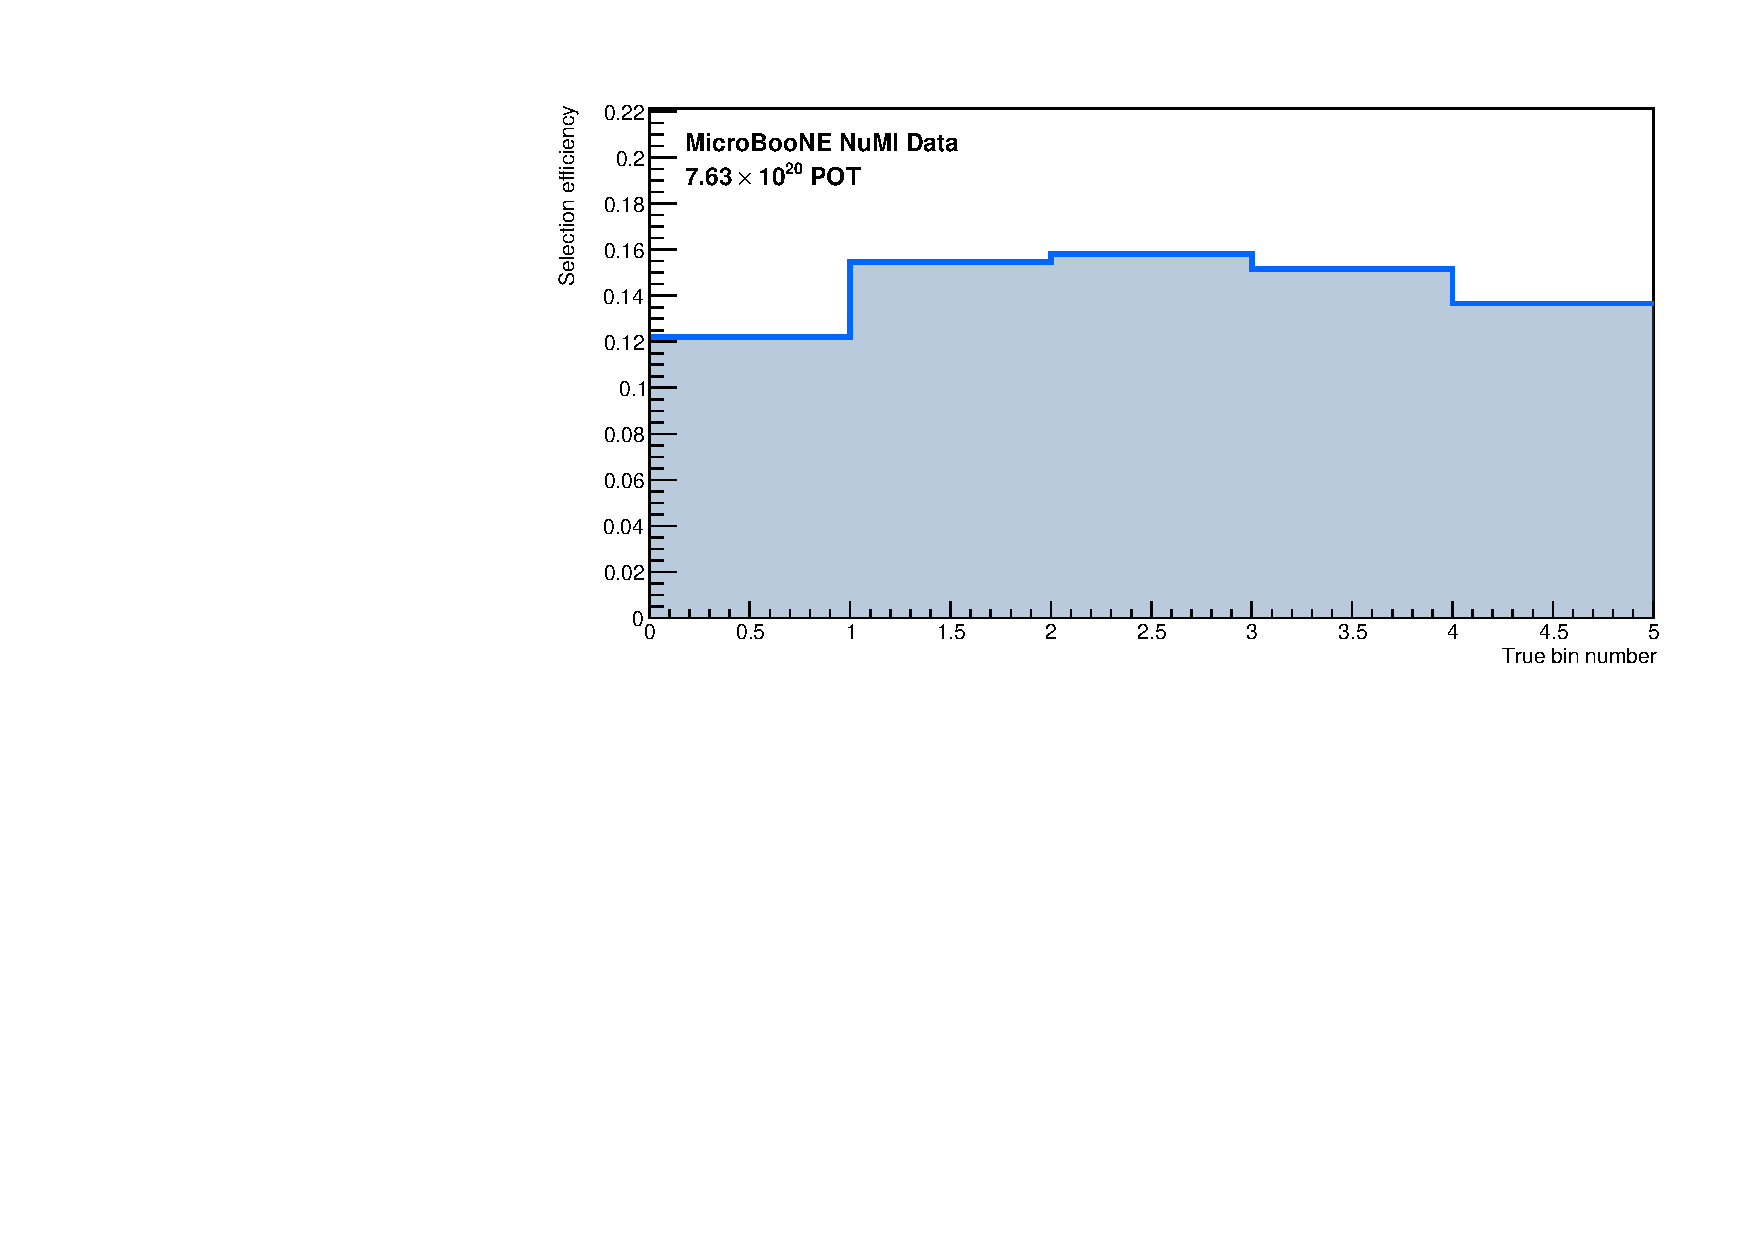
\includegraphics[width=\textwidth]{fw_eff_ppi}
    \caption{$p_\pi$}
  \end{subfigure}
  \hfill
  \begin{subfigure}[b]{0.32\textwidth}
    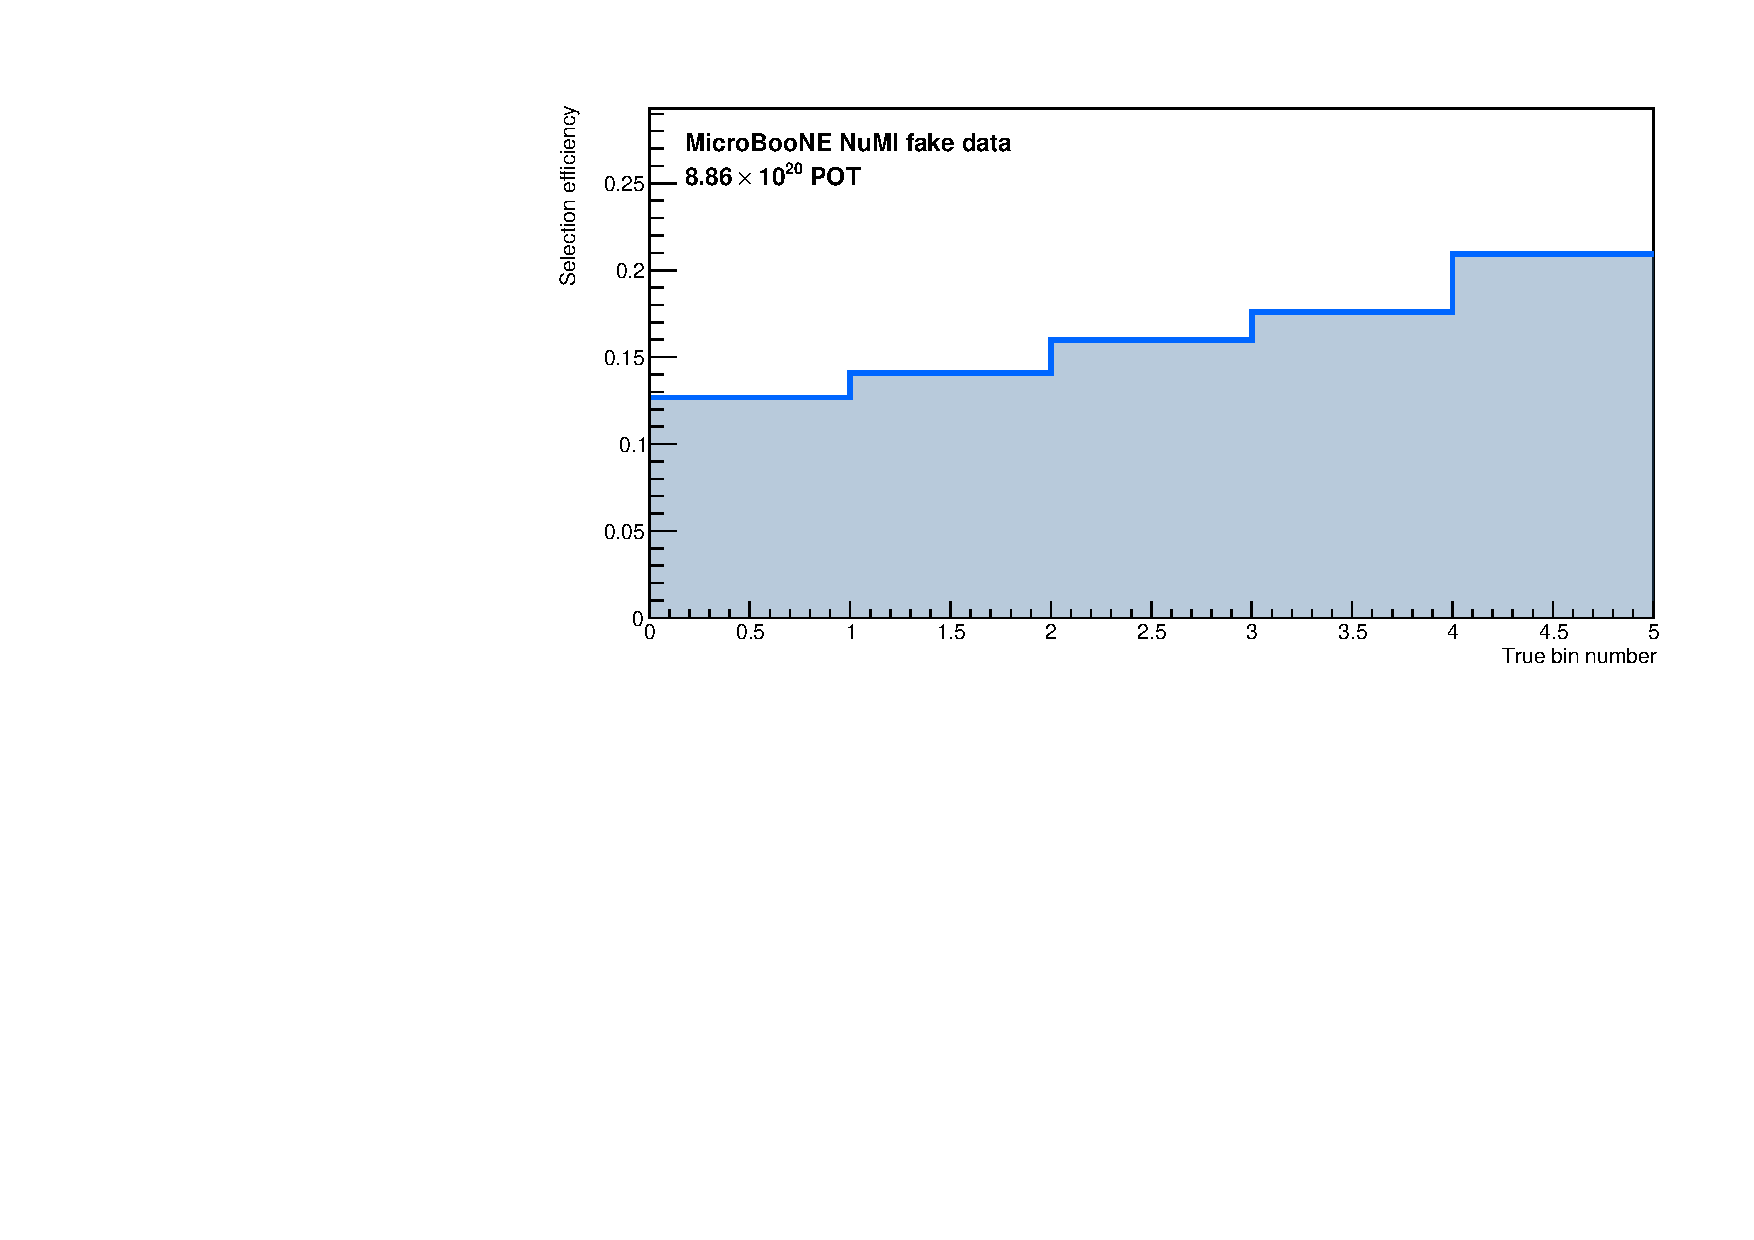
\includegraphics[width=\textwidth]{fw_eff_costhmu}
    \caption{$\cos\theta_\mu$}
  \end{subfigure}\\[6pt]
  \begin{subfigure}[b]{0.32\textwidth}
    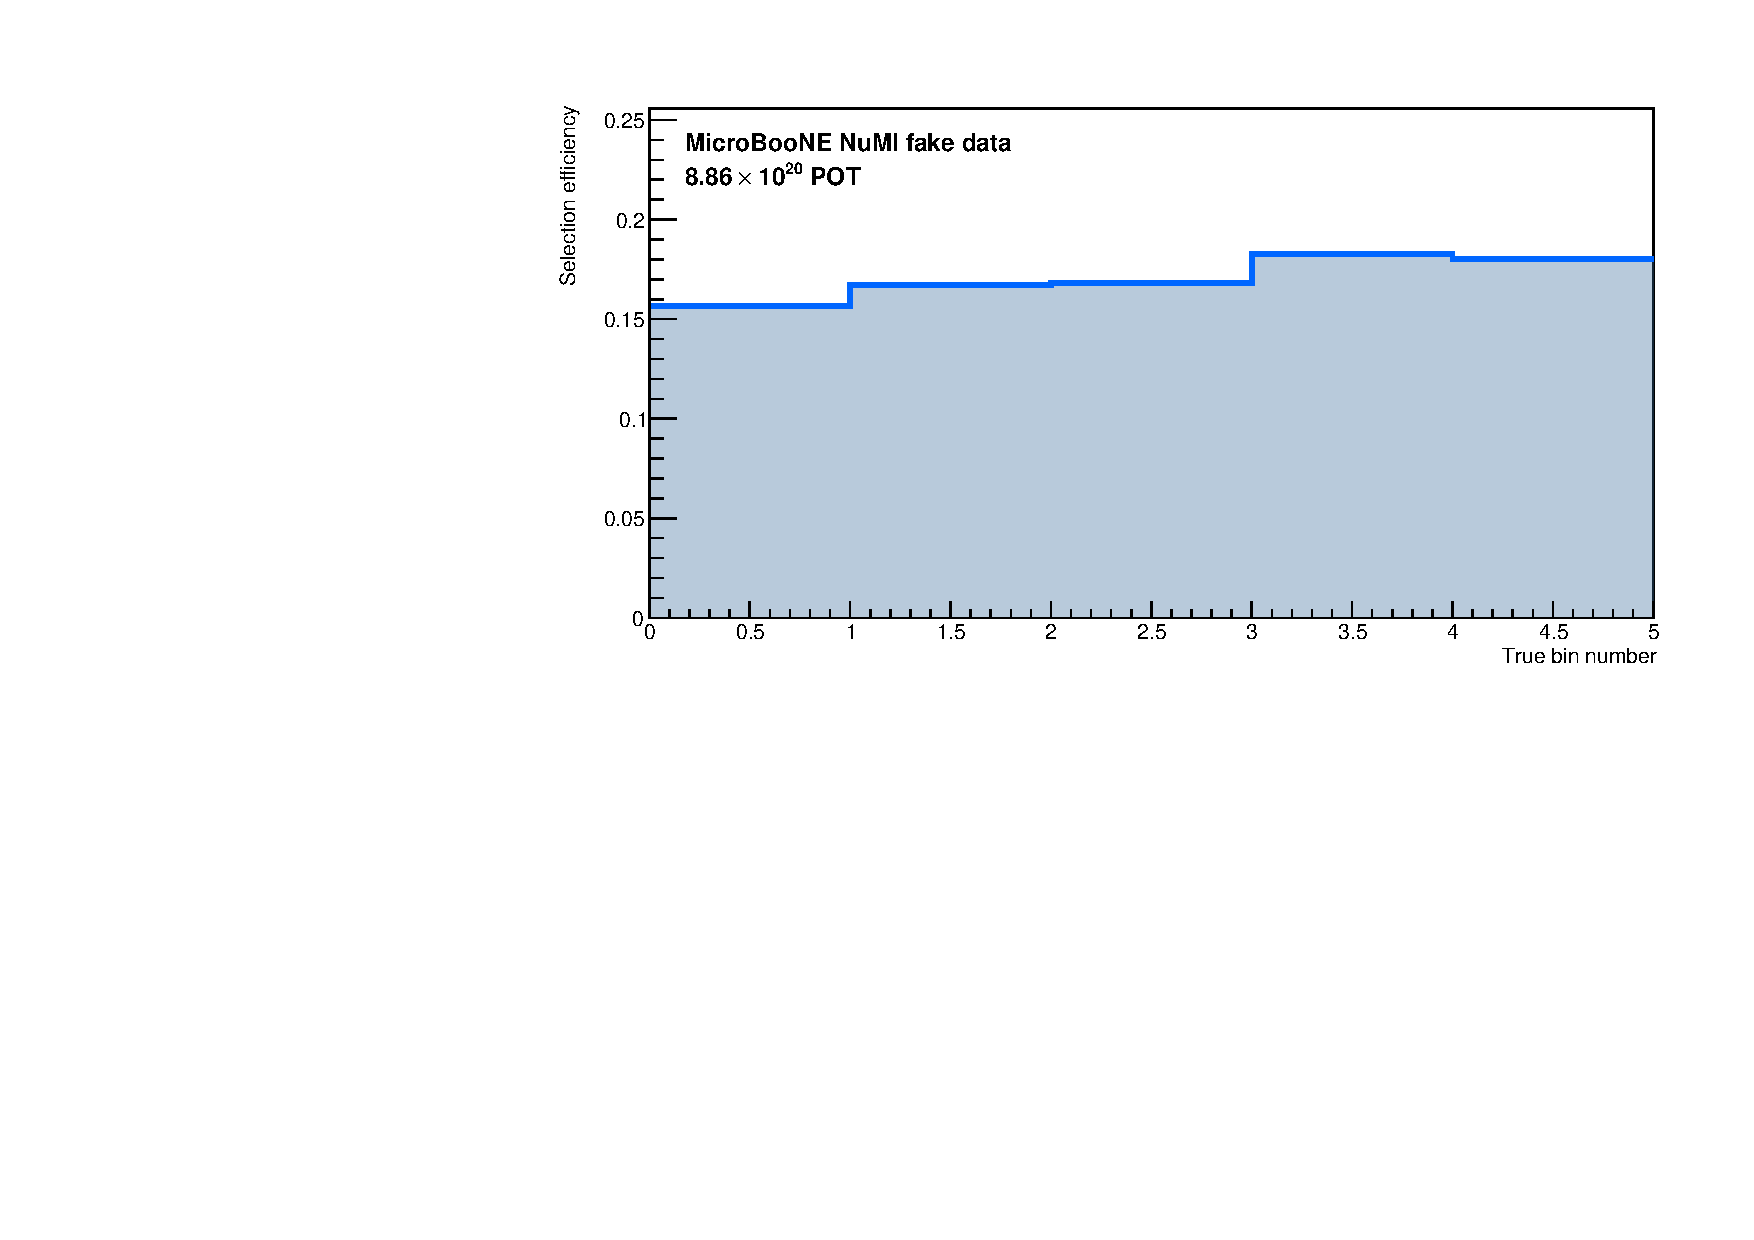
\includegraphics[width=\textwidth]{fw_eff_costhpi}
    \caption{$\cos\theta_\pi$}
  \end{subfigure}
  \hfill
  \begin{subfigure}[b]{0.32\textwidth}
    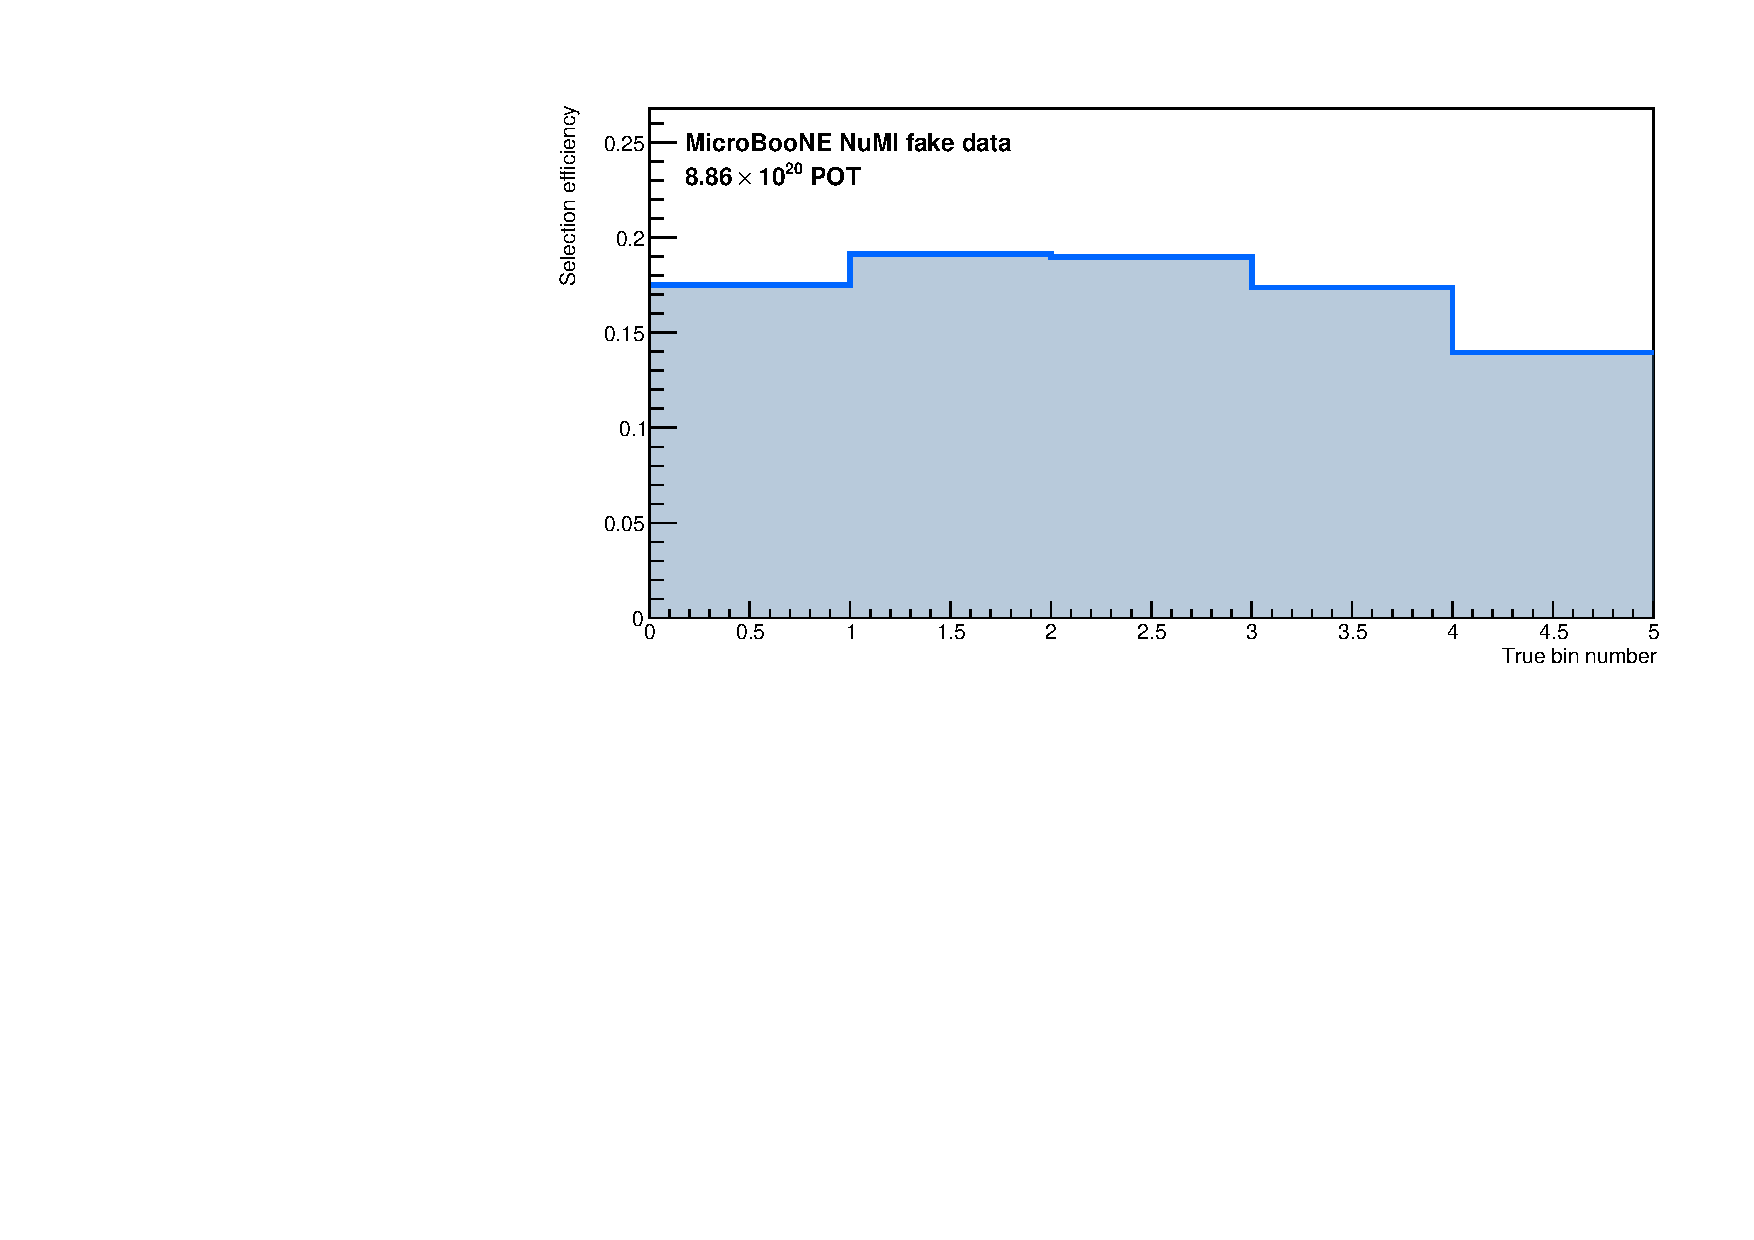
\includegraphics[width=\textwidth]{fw_eff_thmupi}
    \caption{$\theta_{\mu\pi}$}
  \end{subfigure}
  \hfill
  \begin{subfigure}[b]{0.32\textwidth}
    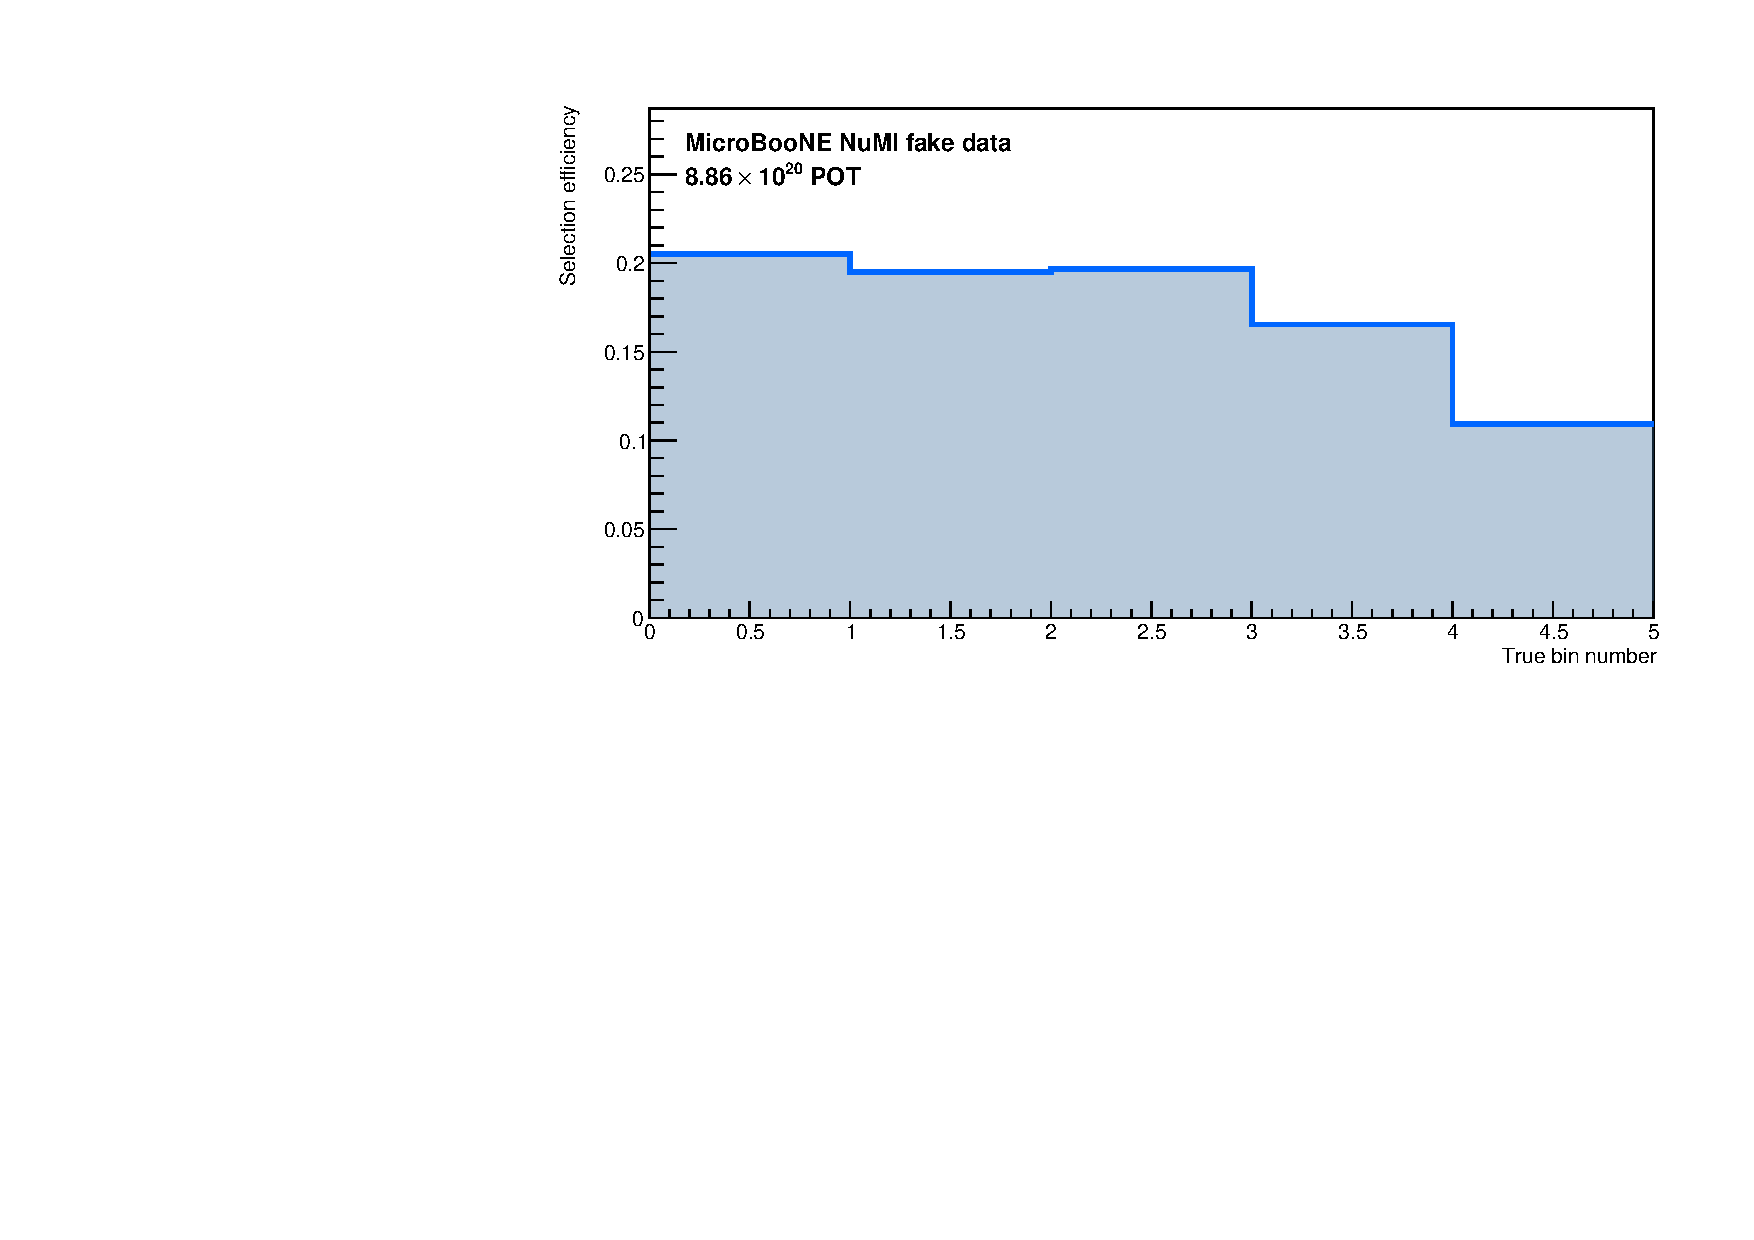
\includegraphics[width=\textwidth]{fw_eff_thetamu}
    \caption{$\theta_\mu$}
  \end{subfigure}
  \caption{Selection efficiency as a function of true observable value, in the
    measured phase space ($p_\mu>0.15$, $p_\pi>0.175\GeVc$,
    $\theta_{\mu\pi}<2.6$~rad).  Efficiency is the ratio of selected to generated
    signal MC ($\varepsilon_i = \sum_j A_{ij}$, integrated over reco bins).  With
    the momentum thresholds and the $2.6$~rad opening-angle cut the efficiency is
    flat at $\sim$13--20\% across all observables; the former $\sim$5\% low-momentum
    turn-on bins and the cosmic-dominated large-angle region are removed.  The
    lowest point is the smallest opening-angle bin ($\sim$9\% efficiency); it is
    retained because it is high-purity ($\sim$58\%), not low-purity.}
  \label{fig:efficiency}
\end{figure}

\subsection{Reconstruction resolution}

Figure~\ref{fig:resolution} shows the reconstruction resolution of each measured
observable, evaluated on selected signal events (GENIE $\nu_\mu$ overlay, measured
phase space).  For the momenta the relative resolution $(\text{reco}-\text{true})/
\text{true}$ is shown; for the angular observables the absolute residual
$(\text{reco}-\text{true})$ is used, since the relative metric diverges as
$\cos\theta\to0$ / $\theta_{\mu\pi}\to0$.  The red points are the mean residual per
true bin; the quoted numbers are the overall mean (bias) and RMS (resolution).

\begin{figure}[H]
  \centering
  \begin{subfigure}[b]{0.32\textwidth}
    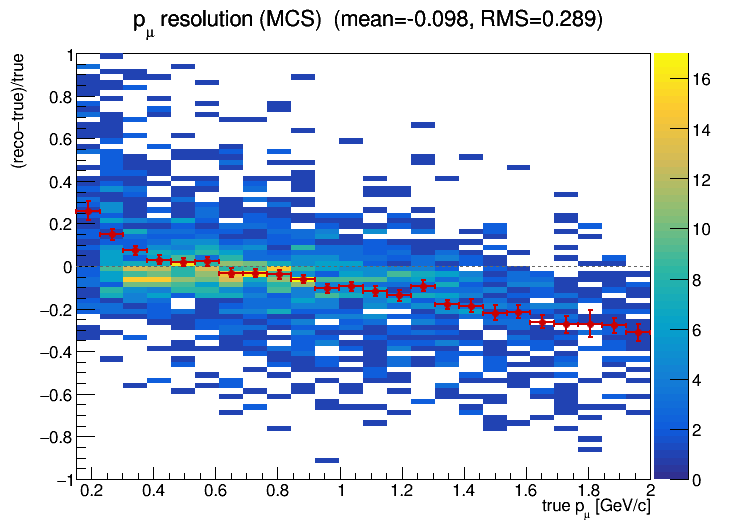
\includegraphics[width=\textwidth]{resolution_pmu_mcs}
    \caption{$p_\mu$ (MCS): bias $-9.8\%$, RMS $30\%$.}
  \end{subfigure}
  \hfill
  \begin{subfigure}[b]{0.32\textwidth}
    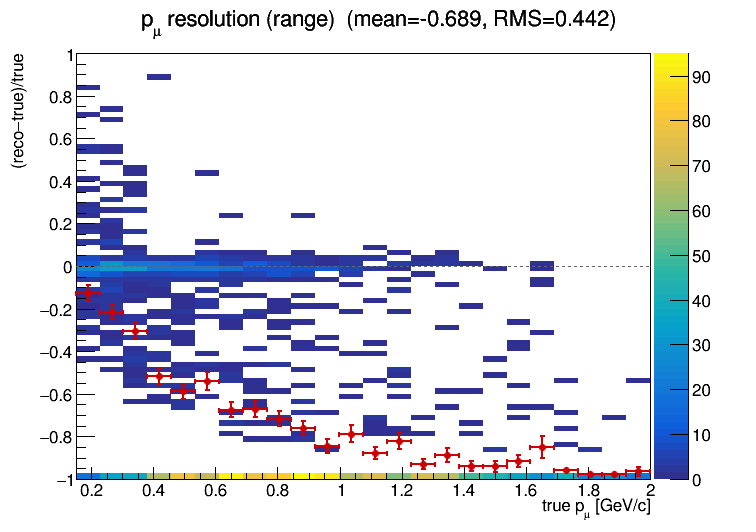
\includegraphics[width=\textwidth]{resolution_pmu_range}
    \caption{$p_\mu$ (range): valid only for contained muons.}
  \end{subfigure}
  \hfill
  \begin{subfigure}[b]{0.32\textwidth}
    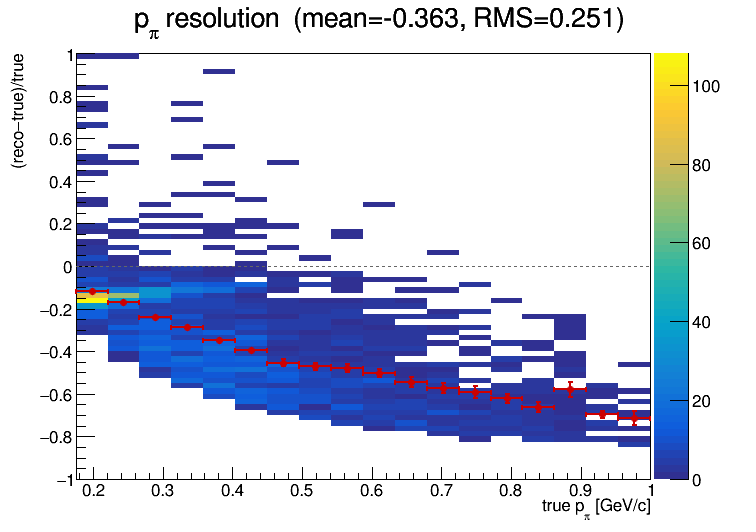
\includegraphics[width=\textwidth]{resolution_ppi}
    \caption{$p_\pi$: bias $-31\%$, RMS $27\%$ (analysis estimator).}
  \end{subfigure}\\[6pt]
  \begin{subfigure}[b]{0.32\textwidth}
    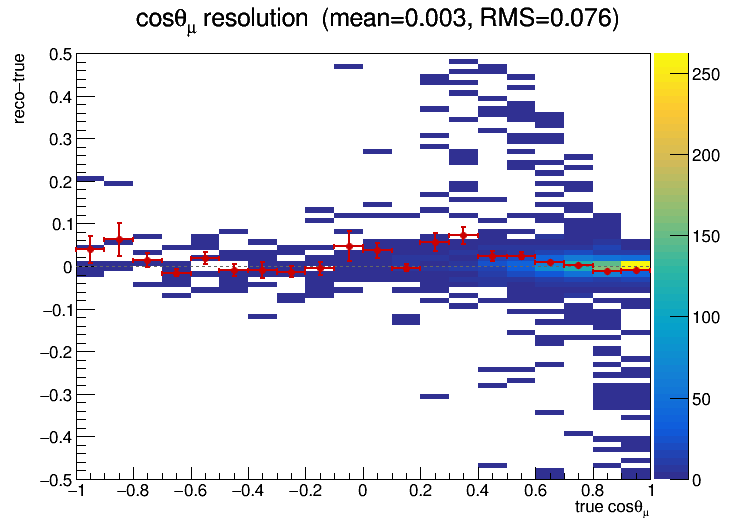
\includegraphics[width=\textwidth]{resolution_costhmu}
    \caption{$\cos\theta_\mu$: RMS $0.076$.}
  \end{subfigure}
  \hfill
  \begin{subfigure}[b]{0.32\textwidth}
    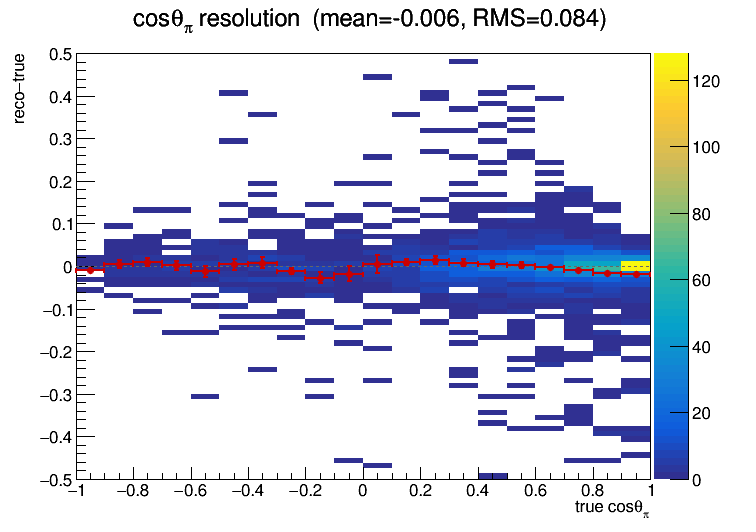
\includegraphics[width=\textwidth]{resolution_costhpi}
    \caption{$\cos\theta_\pi$: RMS $0.095$.}
  \end{subfigure}
  \hfill
  \begin{subfigure}[b]{0.32\textwidth}
    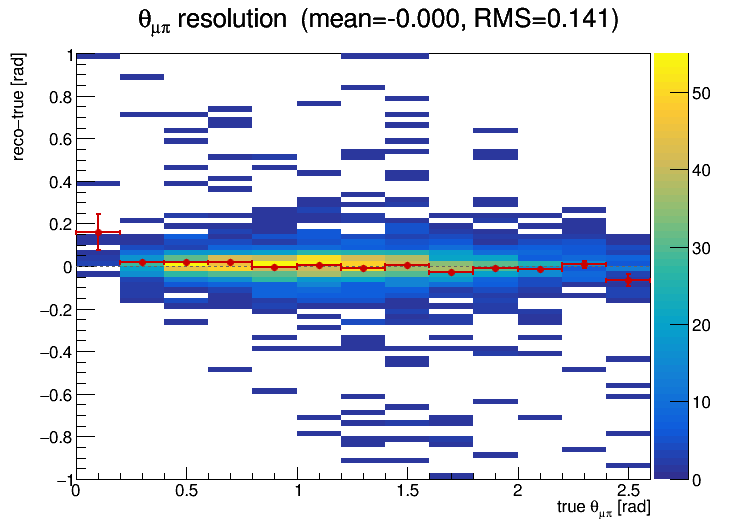
\includegraphics[width=\textwidth]{resolution_thmupi}
    \caption{$\theta_{\mu\pi}$: RMS $0.135$~rad.}
  \end{subfigure}\\[6pt]
  \begin{subfigure}[b]{0.32\textwidth}
    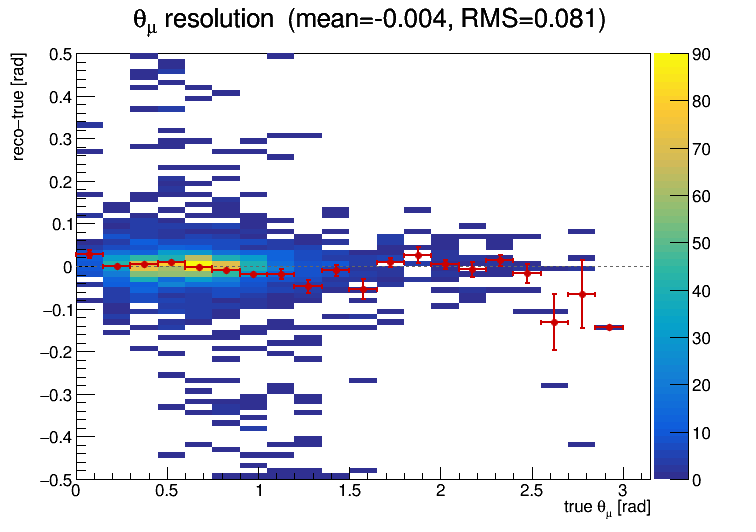
\includegraphics[width=\textwidth]{resolution_thetamu}
    \caption{$\theta_\mu$: RMS $0.081$~rad.}
  \end{subfigure}
  \caption{Reconstruction resolution vs.\ true value, selected signal.  Momenta:
    relative $(\text{reco}-\text{true})/\text{true}$; angles: absolute
    $(\text{reco}-\text{true})$.  Red points: mean residual per true bin.
    $\theta_\mu$ is derived as $\arccos(\cos\theta_\mu)$, exactly as the bin config
    does it, so the panel shows the quantity the analysis bins on; it is unbiased
    ($-0.004$~rad) with RMS $0.081$~rad, the drift below zero above $\sim2.5$~rad being
    a handful of backward-going muons.
    The muon MCS momentum slightly over-estimates at low $p_\mu$ and increasingly
    under-estimates above $\sim$1~GeV/$c$; the range estimator is badly biased for
    \emph{exiting} muons (range $=$ distance to wall), which is why the analysis
    uses range only for contained muons (range-or-MCS).  The pion panel shows the estimator the
    analysis actually bins on, not the raw muon-hypothesis range momentum
    (\suppref{Sec.}{sec:ppi_bias}): mean bias $-31\%$, RMS $27\%$. That average is dominated by
    high momenta; the bias is only $-2\%$ in the first true bin and reaches $-65\%$
    above $0.8$~GeV/$c$; because the reconstructed value saturates near
    $0.34$~GeV/$c$ once pions interact hadronically before stopping. The
    angular variables are essentially unbiased with narrow resolution.}
  \label{fig:resolution}
\end{figure}

\subsection{Model comparison: $\chi^2$ against truth, tune and generators}
\label{sec:chi2}

Table~\ref{tab:chi2_incl} collects the bin-by-bin $\chi^2$ of the unfolded fake data
against each prediction, for every observable and every beam configuration. All
predictions are $A_C$-smeared, so the comparison is made in the measurement space, and the
the nominal configured covariance is used. The \emph{truth} column is the closure test: it is small
throughout (with the caveat on its $p$-values in \S\ref{sec:status_matrix}).

\paragraph{One application of $A_C$.} Every prediction in these tables is smeared by
$A_C$ exactly once, by the extractor; the plotting path reads the smeared curves and does
not smear again. That is verified externally: the released prescription
$\frac{1}{w_i}\sum_j (A_C)_{ij}\,p_j$ applied to the released truth-level predictions
reproduces the released curves to a worst per-bin difference of $1.2\times10^{-10}$
(\suppref{Sec.}{sec:pipeline}). The point matters because a second application would over-smooth
the sharply peaked generators and manufacture an order-of-magnitude $\chi^2$ separation
in the muon-angle observables that is not there: NEUT and NuWro in FHC $\theta_\mu$ give
$8.46/5$ and $9.10/5$, and in $\cos\theta_\mu$ $3.88/5$ and $4.04/5$
(Table~\ref{tab:chi2_incl}), in line with the other observables.

\begin{table}[H]
  \centering
  \caption{$\chi^2$/ndf of the unfolded fake data against each $A_C$-smeared prediction,
    for the inclusive selection. ``truth'' is the fake-data truth (the closure test).}
  \label{tab:chi2_incl}
  \small
  \begin{tabular}{llcccccc}
\toprule
Beam & Observable & truth & uB tune & GENIE & GiBUU & NEUT & NuWro \\
\midrule
    FHC  & $p_\mu$                & $1.45/7$ & $1.54/7$ & $2.51/7$ & $1.69/7$ & $3.08/7$ & $1.42/7$ \\
         & $p_\pi$                & $0.11/2$ & $0.10/2$ & $0.37/2$ & $1.25/2$ & $0.74/2$ & $0.57/2$ \\
         & $\cos\theta_\mu$       & $0.67/5$ & $1.09/5$ & $1.67/5$ & $1.27/5$ & $3.88/5$ & $4.04/5$ \\
         & $\cos\theta_\pi$       & $0.68/5$ & $0.69/5$ & $1.68/5$ & $1.91/5$ & $1.26/5$ & $1.42/5$ \\
         & $\theta_{\mu\pi}$      & $0.30/5$ & $0.86/5$ & $1.20/5$ & $1.44/5$ & $3.87/5$ & $3.82/5$ \\
         & $\theta_\mu$           & $1.52/5$ & $2.14/5$ & $5.55/5$ & $6.07/5$ & $8.46/5$ & $9.10/5$ \\
    \midrule
    RHC  & $p_\mu$                & $0.64/7$ & $2.51/7$ & $3.44/7$ & $2.81/7$ & $3.19/7$ & $3.31/7$ \\
         & $p_\pi$                & $0.02/2$ & $0.01/2$ & $0.56/2$ & $0.30/2$ & $0.25/2$ & $0.11/2$ \\
         & $\cos\theta_\mu$       & $0.35/5$ & $0.37/5$ & $1.11/5$ & $0.24/5$ & $2.71/5$ & $2.67/5$ \\
         & $\cos\theta_\pi$       & $0.49/5$ & $0.43/5$ & $1.27/5$ & $2.86/5$ & $1.79/5$ & $1.08/5$ \\
         & $\theta_{\mu\pi}$      & $0.19/5$ & $0.34/5$ & $2.52/5$ & $3.54/5$ & $0.46/5$ & $1.08/5$ \\
         & $\theta_\mu$           & $0.12/5$ & $0.21/5$ & $0.78/5$ & $0.34/5$ & $5.60/5$ & $5.76/5$ \\
    \midrule
    comb & $p_\mu$                & $0.41/7$ & $0.74/7$ & $2.08/7$ & $0.86/7$ & $1.46/7$ & $0.98/7$ \\
         & $p_\pi$                & $0.01/2$ & $0.01/2$ & $0.45/2$ & $0.92/2$ & $0.47/2$ & $0.30/2$ \\
         & $\cos\theta_\mu$       & $0.05/5$ & $0.09/5$ & $0.84/5$ & $0.47/5$ & $3.27/5$ & $2.92/5$ \\
         & $\cos\theta_\pi$       & $0.73/5$ & $0.54/5$ & $1.84/5$ & $2.72/5$ & $1.43/5$ & $1.23/5$ \\
         & $\theta_{\mu\pi}$      & $0.06/5$ & $0.54/5$ & $1.76/5$ & $2.64/5$ & $2.41/5$ & $2.89/5$ \\
         & $\theta_\mu$           & $0.56/5$ & $0.83/5$ & $3.16/5$ & $4.71/5$ & $8.20/5$ & $7.87/5$ \\
\bottomrule
\end{tabular}
\end{table}

\begin{table}[H]
  \centering
  \caption{The same comparison for the muon angle in both parameterisations. The two
    binnings span the same full range but are different partitions of it: the $\theta_\mu$
    edges ($0.43$, $0.62$, $0.84$, $1.17$~rad) are not the $\arccos$ images of the
    $\cos\theta_\mu$ edges ($0.45$, $0.64$, $0.86$, $1.10$~rad). The $\theta_\mu$
    $\chi^2$ are systematically the larger for every column including the truth, a
    consequence of the different partition and of $A_C$. Model statements in this note
    are made on $\cos\theta_\mu$; $\theta_\mu$ is released as the second
    parameterisation.}
\label{tab:chi2_theta}
  \small
  \begin{tabular}{llcccccc}
\toprule
Beam & Variable & truth & uB tune & GENIE & GiBUU & NEUT & NuWro \\
\midrule
FHC & $\cos\theta_\mu$   & $0.67/5$ & $1.09/5$ & $1.67/5$ & $1.27/5$ & $3.88/5$ & $4.04/5$ \\
FHC & $\theta_\mu$       & $1.52/5$ & $2.14/5$ & $5.55/5$ & $6.07/5$ & $8.46/5$ & $9.10/5$ \\
\midrule
RHC & $\cos\theta_\mu$   & $0.35/5$ & $0.37/5$ & $1.11/5$ & $0.24/5$ & $2.71/5$ & $2.67/5$ \\
RHC & $\theta_\mu$       & $0.12/5$ & $0.21/5$ & $0.78/5$ & $0.34/5$ & $5.60/5$ & $5.76/5$ \\
\midrule
Comb & $\cos\theta_\mu$   & $0.05/5$ & $0.09/5$ & $0.84/5$ & $0.47/5$ & $3.27/5$ & $2.92/5$ \\
Comb & $\theta_\mu$       & $0.56/5$ & $0.83/5$ & $3.16/5$ & $4.71/5$ & $8.20/5$ & $7.87/5$ \\
\bottomrule
\end{tabular}
\end{table}

\section{Full-exposure results: FHC, RHC, and combined}
\label{sec:results}
\label{sec:rhc}

\subsection{Scope and status of each result}
\label{sec:status_matrix}

Table~\ref{tab:inventory} is the inventory of everything this analysis has extracted, generated
from the release index so that it cannot drift from what was produced. The fifty-one differential
extractions in the release --- six inclusive and eleven proton-tagged observables, each in three
configurations --- carry the systematic covariance of the nominal configured uncertainty model,
detector variations included. ``Nominal configured'' is meant strictly: the identified terms that
are \emph{not} in it are listed in \S\ref{sec:limitations}, and the phrase should not be read as a
complete accounting of every uncertainty this measurement has.

% generated by report/tools/inventory.py -- do not edit
\begin{table}[H]
  \centering
  \caption{Every extraction this analysis has produced, generated from the release index (\texttt{report/tools/inventory.py}). The extraction count is one per observable and configuration. The withdrawn products are present in the release directory and must not be quoted (Appendix~\ref{app:withdrawn}).}
  \label{tab:inventory}
  \small
  \begin{tabular}{lccl}
    \toprule
    Family & Observables & Extractions & Status \\
    \midrule
    Inclusive differential & 6 & 18 & primary \\
    Inclusive one-bin total & 1 & 3 & primary \\
    Proton-tagged differential & 11 & 33 & secondary \\
    Proton-tagged one-bin total & 1 & 3 & secondary \\
    Proton-tagged angular ($\theta_p$, $\theta_{\pi p}$) & 2 & 6 & proposed secondary$^{1}$ \\
    Two-dimensional pairs & 8 & 24 & two proposed, combined only$^{1}$ \\
    \midrule
    \multicolumn{4}{l}{\emph{Of the above, withdrawn --- do not quote}} \\
    Differential $W_{\pi p}$ & 1 & 3 & withdrawn \\
    Five-bin $d\sigma/dp_\pi$ & 1 & --- & withdrawn, not in the release \\
    \bottomrule
  \end{tabular}
  \par\smallskip\noindent{\footnotesize $^{1}$ Produced after the release directory was written, so not indexed there.}
\end{table}

 The proton-tagged
detector terms run from $10.5\%$ to $108.5\%$ with a median of $33.0\%$, against
$15.6\%$--$35.0\%$ for the inclusive results; the wide range is the sparse six-bin
samples, where the unfolding amplifies them.

The proton-tagged results are secondary scope because the exposure does not support
the differential $W_{\pi p}$ shape at any binning, the proton-mistag background lacks a
dedicated inverted-proton-PID control region (\suppref{Sec.}{sec:cr_1p_scope}), and ensemble
coverage has not been demonstrated for this sparser family (\S\ref{sec:limitations}).

The status of every product --- primary, secondary, proposed, validation-only or withdrawn ---
is given once, in the status box of \S\ref{sec:status}, and the inventory above is generated from
the release index. The two are the controlled vocabulary of this note; where a table or caption
below says ``validation product'', it means a secondary-scope extraction that is complete but not
proposed for approval in this review, and ``diagnostic'' means a distribution shown only to
explain why a result is withdrawn.


\paragraph{What the reader should know before the tables.}
Three points condition how the numbers below are read, and are established in
\suppref{Sec.}{sec:supp_caveats}. \emph{First}, $d\sigma/dp_\pi$ is released in two bins only:
charged pions interact before ranging out, so the reconstructed momentum saturates near
$0.34$~GeV/$c$ and no finer binning survives the migration criterion; the upper bin is open-ended
and its released density represents a bin integral. \emph{Second}, the closure $\chi^2$ quoted with
each extraction uses the nominal configured covariance, so its $p$-values are not a sensitive test
of the extraction --- they confirm consistency and nothing more. \emph{Third}, an ensemble of
independent Poisson realisations carried through the whole chain gives per-bin pull widths of
$0.97$--$1.08$, so the quoted statistical uncertainties are correctly sized; the study covers three
extractions in one configuration, and RHC and the proton-tagged family have not been tested.


This is the primary result of the analysis: the CC$1\mu1\pi^\pm$ cross section
extracted over the full available exposure in forward horn current (FHC), reverse
horn current (RHC), and their combination, all on Poisson-thrown central-value fake
data. The FHC measurement uses Runs~1, 2, 4 and 5 (data POT
$8.857\times10^{20}$); RHC uses Runs~1, 2, 3, 4a, 4b, 4c ($1.108\times10^{21}$); the
combined measurement uses all fourteen overlay files at the joint POT
$1.994\times10^{21}$. All three close cleanly against the $A_C$-smeared truth for
every observable (Tables~\ref{tab:fhc}--\ref{tab:comb}); the differential results are
shown in Figs.~\ref{fig:dsigma_current}--\ref{fig:dsigma_comb}.

\begin{center}\small
\captionof{table}{FHC (Runs 1, 2, 4, 5; data POT $8.857\times10^{20}$): integrated cross section, the two largest systematic terms, the total, and the fake-data closure against $A_C$-smeared truth. All values are read from the released covariance and results table; the anatomy of the flux term is in \S\ref{sec:fluxanatomy}.}
    \label{tab:fhc}
\begin{tabular}{lccccc}
\toprule
Observable & $\sigma_\mathrm{int}$ & Flux & Detector & Total & Closure $\chi^2/\mathrm{ndf}$ \\
\midrule
      $p_\mu$            & $0.838$ & $28.0\%$ & $24.7\%$ & $40.7\%$ & $1.45/7$ ($p=0.98$) \\
      $p_\pi$            & $0.822$ & $32.5\%$ & $30.3\%$ & $50.2\%$ & $0.11/2$ ($p=0.95$) \\
      $\cos\theta_\mu$   & $0.754$ & $28.0\%$ & $28.3\%$ & $42.0\%$ & $0.67/5$ ($p=0.98$) \\
      $\cos\theta_\pi$   & $0.674$ & $27.0\%$ & $22.9\%$ & $38.8\%$ & $0.68/5$ ($p=0.98$) \\
      $\theta_{\mu\pi}$  & $0.819$ & $28.3\%$ & $19.6\%$ & $36.5\%$ & $0.30/5$ ($p=1.00$) \\
      $\theta_\mu$       & $0.960$ & $24.7\%$ & $15.6\%$ & $31.0\%$ & $1.52/5$ ($p=0.91$) \\
\bottomrule
\end{tabular}
\end{center}

We extend the measurement to the reverse-horn-current beam as both a
standalone measurement and a combined $\nu_\mu+\bar\nu_\mu$ result.
The RHC \emph{flux} is $\bar\nu_\mu$-dominant ($54.6\%$ $\bar\nu_\mu$, versus FHC's
$35\%$), with  $>\!60$~MeV integrals
$\Phi_{\nu_\mu}^\mathrm{RHC}=2.923\times10^{-10}$,
$\Phi_{\bar\nu_\mu}^\mathrm{RHC}=3.523\times10^{-10}$, total
$6.446\times10^{-10}~\mathrm{cm}^{-2}\mathrm{POT}^{-1}$ (the FHC-convention
computation reproduces the authoritative FHC values exactly). The \emph{measured
event rate}, however, remains $\nu_\mu$-dominant ($76\%$ $\nu_\mu$, $20\%$
$\bar\nu_\mu$) because the $\nu_\mu$ cross section is $\sim\!2$--$3\times$ larger
than the $\bar\nu_\mu$ one. The RHC overlays (Runs~1, 2, 3, 4a, 4b, 4c) are all
verified as genuine $\nu_\mu$ overlays (flavour composition $100\%$ $\nu_\mu+\bar\nu_\mu$ at truth level, events per POT uniform across files) and processed, $4.05\times10^{6}$ events,
combined MC POT $1.546\times10^{22}$, mutually consistent
($2.62\times10^{-16}$ events/POT) with the PPFX weights, covering the full RHC
exposure (Run~3 is the largest period, $5.52\times10^{21}$~MC~POT and $1.44\times10^{6}$
events). Native Run-4 RHC detector-variation samples (the standard eight-knob set:
light-yield down/Rayleigh, recombination, space charge, and the four wire-modification
variations) provide the RHC detector systematic, verified as genuine $\nu_\mu$ overlays
with a uniform $3.80\times10^{-16}$ events/POT across all knobs. The RHC dirt prediction
uses the FHC dirt overlay, scaled to the RHC exposure, as no RHC dirt sample exists. The standalone result below uses Poisson-thrown central-value
fake data at the RHC data POT $1.108\times10^{21}$. The generator
predictions are re-averaged to the RHC flux composition; the combined FHC$+$RHC
predictions are the fluence-weighted combination of the two horn modes
($0.458$~FHC $/\,0.542$~RHC, each mode weighted by $\Phi_\mathrm{tot}\times$POT).

The combined FHC$+$RHC measurement uses the summed $14$-file response over the full
exposure ($5.6\times10^{6}$ events, combined data POT
$D_\mathrm{comb}=1.994\times10^{21}=D_\mathrm{FHC}+D_\mathrm{RHC}$), with each horn
mode normalised to its \emph{own} data exposure. Each mode's simulation and detector-variation samples are scaled to that mode's own data exposure, so the combined prediction weights the modes by data exposure ($0.80{:}1$) rather than by simulated exposure ($0.62{:}1$), and the fake data is thrown at the matching rate.

The joint \emph{flux systematic} needs no hand-built cross-horn correlation. All
fourteen numuMC files carry the \emph{same} $600$ PPFX multisim universes --- a universe being one alternative prediction with a systematic parameter varied, a multisim a set of hundreds of them drawn from the parameter uncertainties --- which the universe maker accumulates index-matched across both horn
modes in a single chain, so universe $u$ is the same hadron-production draw in FHC
and RHC. Per-universe summing therefore propagates one parameter draw through both
beam configurations and lets each mode's flux response set the result, capturing the
physical (not unit) cross-horn correlation automatically. The detector
variations are carried per mode, the Run-4 FHC and Run-4 RHC samples of each knob
accumulated under one label, so the combined detector term is exposure-weighted like the
central value. The combined closure passes for every observable (Table~\ref{tab:comb}), with an unfolded flux systematic of
$24$--$30\%$ of the same size as the standalone FHC ($25$--$33\%$) and RHC ($25$--$28\%$)
values (Tables~\ref{tab:fhc}--\ref{tab:comb}), as expected for a common flux model
propagated through three similarly conditioned responses.

The standalone RHC extraction (native Run-4 RHC detector variations) closes cleanly
for every observable (Table~\ref{tab:rhc}): the realised $A_C$-smeared truth is recovered
with $\chi^2\le0.7$ on two to seven degrees of freedom and $p\ge0.98$ throughout. The
reconstructed-level flux uncertainty is $\sim\!15\%$, below the FHC $\sim\!17\%$, because
the $\bar\nu_\mu$-dominant flux carries a smaller PPFX hadron-production uncertainty; the
unfolded flux term ($25$--$28\%$, Table~\ref{tab:rhc}) is nevertheless comparable to the
FHC one, since the background subtraction multiplies both by the same $1+B/S$
(\S\ref{sec:fluxanatomy}).

\begin{center}\small
\captionof{table}{RHC (Runs 1, 2, 3, 4; data POT $1.1082\times10^{21}$): integrated cross section, the two largest systematic terms, the total, and the fake-data closure against $A_C$-smeared truth. All values are read from the released covariance and results table; the anatomy of the flux term is in \S\ref{sec:fluxanatomy}.}
    \label{tab:rhc}
\begin{tabular}{lccccc}
\toprule
Observable & $\sigma_\mathrm{int}$ & Flux & Detector & Total & Closure $\chi^2/\mathrm{ndf}$ \\
\midrule
      $p_\mu$            & $0.690$ & $27.6\%$ & $21.5\%$ & $37.7\%$ & $0.64/7$ ($p=1.00$) \\
      $p_\pi$            & $0.748$ & $28.4\%$ & $34.7\%$ & $48.6\%$ & $0.01/2$ ($p=0.99$) \\
      $\cos\theta_\mu$   & $0.733$ & $25.8\%$ & $35.0\%$ & $46.3\%$ & $0.35/5$ ($p=1.00$) \\
      $\cos\theta_\pi$   & $0.615$ & $25.2\%$ & $25.5\%$ & $38.5\%$ & $0.49/5$ ($p=0.99$) \\
      $\theta_{\mu\pi}$  & $0.831$ & $25.2\%$ & $16.6\%$ & $32.6\%$ & $0.18/5$ ($p=1.00$) \\
      $\theta_\mu$       & $0.805$ & $25.6\%$ & $22.4\%$ & $36.1\%$ & $0.12/5$ ($p=1.00$) \\
\bottomrule
\end{tabular}
\end{center}

\begin{center}\small
\captionof{table}{Combined (data POT $1.9939\times10^{21}$): integrated cross section, the two largest systematic terms, the total, and the fake-data closure against $A_C$-smeared truth. All values are read from the released covariance and results table; the anatomy of the flux term is in \S\ref{sec:fluxanatomy}.}
    \label{tab:comb}
\begin{tabular}{lccccc}
\toprule
Observable & $\sigma_\mathrm{int}$ & Flux & Detector & Total & Closure $\chi^2/\mathrm{ndf}$ \\
\midrule
      $p_\mu$            & $0.827$ & $24.2\%$ & $21.4\%$ & $34.9\%$ & $0.41/7$ ($p=1.00$) \\
      $p_\pi$            & $0.775$ & $30.2\%$ & $30.8\%$ & $47.9\%$ & $0.01/2$ ($p=1.00$) \\
      $\cos\theta_\mu$   & $0.812$ & $25.7\%$ & $23.8\%$ & $37.3\%$ & $0.04/5$ ($p=1.00$) \\
      $\cos\theta_\pi$   & $0.658$ & $25.6\%$ & $22.5\%$ & $37.1\%$ & $0.73/5$ ($p=0.98$) \\
      $\theta_{\mu\pi}$  & $0.879$ & $25.7\%$ & $17.7\%$ & $33.2\%$ & $0.06/5$ ($p=1.00$) \\
      $\theta_\mu$       & $0.851$ & $25.2\%$ & $20.6\%$ & $34.4\%$ & $0.56/5$ ($p=0.99$) \\
\bottomrule
\end{tabular}
\end{center}

\begin{figure}[H]\centering
  \blindfig[0.98\textwidth]{dsigma_FHC5}
  \caption{Differential cross sections $d\sigma/dx$ for the six released distributions on the
    current Poisson-thrown central-value fake data, FHC full exposure: unfolded fake
    data (black points), $A_C$-smeared fake-data truth (grey dashed), the MicroBooNE
    tune (black solid), and the four generator predictions (GENIE, GiBUU, NEUT,
    NuWro). The unfolded points recover the injected truth for every observable, the
    same closure summarised in Table~\ref{tab:fhc}.}
  \label{fig:dsigma_current}
\end{figure}

\begin{figure}[H]\centering
  \blindfig[0.98\textwidth]{dsigma_RHCFULL}
  \caption{Standalone RHC ($\bar\nu_\mu$-dominant) differential cross sections on the
    current Poisson-thrown fake data, with the RHC-flux-averaged generator
    predictions. Same layout as Fig.~\ref{fig:dsigma_current}.}
  \label{fig:dsigma_rhc}
\end{figure}

\begin{figure}[H]\centering
  \blindfig[0.98\textwidth]{dsigma_COMB}
  \caption{Combined FHC$+$RHC ($\nu_\mu+\bar\nu_\mu$) differential cross sections on
    the current per-mode-normalised fake data, with the fluence-weighted combined
    generator predictions.}
  \label{fig:dsigma_comb}
\end{figure}

\begin{center}\small
\captionof{table}{Integrated (unfolded) cross section $\sigma_\mathrm{int}$ over the
  measured phase space, for each observable and configuration (current fake data,
  five-bin forward-split $\cos\theta_\pi$ and coarsened $\theta_{\mu\pi}$ binning, per-configuration flux;
  $10^{-38}$~cm$^2$/Ar). The value differs between observables because the Wiener-SVD
  additional-smearing $A_C$ is not norm-preserving; the D'Agostini cross-check
  (\suppref{Sec.}{sec:crosschecks}) recovers a flat, $23$--$31\%$ higher total, consistent
  with the spread being a smearing effect (the $A_C$ row sums of \S\ref{sec:ac_rowsums}
  establish it directly). The MC normalisation is evaluated run by run from each run's exposure. The final row gives the alternative
  muon-angle parameterisation $\theta_\mu$ (\suppref{Sec.}{sec:thetavar}), complete for
  all three configurations; no $\theta_\pi$ parameterisation is extracted. (Values are fake-data closures; the signal is
  $\nu_\mu+\bar\nu_\mu$, so the RHC flux-average is not expected to lie far below FHC.) }
\label{tab:sigint_all}
\begin{tabular}{lccc}
\toprule
Observable & FHC & RHC & Combined \\
\midrule
$p_\mu$           & $0.838$ & $0.690$ & $0.827$ \\
$p_\pi$           & $0.822$ & $0.748$ & $0.775$ \\
$\cos\theta_\mu$  & $0.754$ & $0.733$ & $0.812$ \\
$\cos\theta_\pi$  & $0.674$ & $0.615$ & $0.658$ \\
$\theta_{\mu\pi}$ & $0.819$ & $0.831$ & $0.879$ \\
\midrule
$\theta_\mu$      & $0.960$ & $0.805$ & $0.851$ \\
\bottomrule
\end{tabular}
\end{center}

\paragraph{Uncertainties shown.}
Every differential cross section and every integrated value quoted in this note carries
\emph{both} statistical and systematic uncertainties. The error bars on the unfolded points
are the square root of the diagonal of the \emph{total} covariance matrix, propagated
through the unfolding: flux (PPFX multisims), cross-section (GENIE multisims and unisims, a unisim being a single $\pm1\sigma$ variation of one parameter),
detector variations~\cite{uboone_detvar}, hadron re-interaction~\cite{geant4reweight}, POT counting and target number, together with
the data, MC and EXT statistical terms. For $p_\mu$ in FHC the bin-averaged total is
$40.7\%$ (Table~\ref{tab:systbreak}), dominated by flux ($28.0\%$) and detector
($24.7\%$), with data statistics $14.3\%$ and cross-section $10.7\%$. The one-bin total
cross section of \S\ref{sec:total_xsec} carries its own breakdown from the same universes,
written there as systematic $\oplus$ data-statistical (FHC: $38.5\%\oplus4.3\%$); without
regularisation its flux and detector terms are not amplified.


\subsection{The two-region \texorpdfstring{$p_\pi$}{p pi} measurement}
\label{sec:ppi_two_region}

Because the upper pion-momentum bin is open-ended, the $p_\pi$ result is reported as two
bin-integrated cross sections rather than as a spectrum. These are the quantities to compare a
prediction with; the differential form exists only so that the result can be drawn next to the
others, and it carries the reporting width described in Appendix~\ref{app:binning}.

\begin{table}[H]
  \centering
  \caption{The $p_\pi$ result as bin integrals, $10^{-38}$~cm$^2$/Ar, on fake data. The upper region
    is open-ended; no width is assigned to it here and none is needed. Uncertainties are the total
    of the nominal configured covariance.}
  \label{tab:ppi_partial_main}
  \small
  \begin{tabular}{lccc}
    \toprule
    Region & FHC & RHC & Combined \\
    \midrule
    $\sigma(0.175<p_\pi<0.205$~GeV/$c)$ & $0.059\pm0.041$ & $0.054\pm0.034$ & $0.062\pm0.038$ \\
    $\sigma(p_\pi>0.205$~GeV/$c)$ & $0.764\pm0.293$ & $0.694\pm0.268$ & $0.713\pm0.270$ \\
    \bottomrule
  \end{tabular}
\end{table}

\subsection{How far \texorpdfstring{$A_C$}{A C} is from preserving normalisation}
\label{sec:ac_rowsums}

Because the Wiener-SVD result estimates $A_C x_{\rm true}$ rather than $x_{\rm true}$,
and $A_C$ is not norm preserving, summing the differential result over its bins does not
give the physical total cross section. This subsection quantifies the effect.

The row sums of $A_C$ are the diagnostic used here: they give the response to a flat
bin-integrated truth, for which a row summing to unity passes the normalisation of that
bin through unchanged and a row summing to $0.2$ passes one fifth of it. For a non-flat
prediction the output of bin $i$ is $\sum_j (A_C)_{ij}\,t_j$, which depends on the
individual elements and on the shape of $t$; the row sums describe the dominant behaviour,
and the model-specific integral factors of \S\ref{sec:chain} ($0.76$--$0.79$ for the four
generators in FHC $p_\mu$) show how far it carries over.

\begin{center}
\small
\begin{tabular}{lccc}
\toprule
Observable & FHC & RHC & combined \\
\midrule
$p_\mu$ & $0.66$--$0.91$ & $0.58$--$0.99$ & $0.68$--$1.01$ \\
$p_\pi$ (2-bin) & $0.35$--$0.54$ & $0.40$--$0.51$ & $0.29$--$0.54$ \\
$\cos\theta_\mu$ & $0.17$--$0.39$ & $0.05$--$0.45$ & $0.09$--$0.43$ \\
$\cos\theta_\pi$ & $0.68$--$0.77$ & $0.70$--$0.84$ & $0.71$--$0.83$ \\
$\theta_{\mu\pi}$ & $0.52$--$1.03$ & $0.58$--$1.15$ & $0.63$--$1.21$ \\
$\theta_\mu$ & $0.58$--$0.78$ & $0.22$--$1.16$ & $0.53$--$0.67$ \\
\bottomrule
\end{tabular}
\end{center}

\noindent The suppression is large (inclusive $\cos\theta_\mu$ has a row sum as low as
$0.05$ in RHC) and differs strongly between observables, which is why the integrated
cross section obtained by summing a differential result varies from observable to
observable while the physical total cannot; the D'Agostini cross-check, whose integral
is flat across observables, confirms that the spread is the smearing
(\suppref{Sec.}{sec:crosschecks}). The proton-tagged row sums, and the two matrices whose
least-determined row sums to a small negative value (RHC $W_{\pi p}$ and the first
$\cos\theta_\mu$ bin of the proton-tagged RHC sample), are tabulated and discussed in
\suppref{Sec.}{sec:supp_ac}; a negative row is not forbidden for a regularisation
operator, but those two rows should be read with corresponding caution.

\paragraph{Numerical data release.}
All fifty-one differential extractions are released in \texttt{report/data\_release/},
indexed by \texttt{index\_extractions.tsv}: the additional-smearing matrix, the full
per-component covariance in cross-section units, and \texttt{curves\_*.tsv} holding the
unfolded data together with every model curve shown here. The six one-bin totals, with
their uncertainty breakdown and realised truth, are in \texttt{total\_xsec.tsv}.

A prediction supplied as a per-bin cross section is compared with these results by
\[
  \left(\frac{d\sigma}{dx}\right)^{\rm smeared}_i
  \;=\; \frac{1}{w_i}\sum_j \left(A_C\right)_{ij}\, p_j ,
\]
with $p_j$ the predicted cross section in true bin $j$ and $w_i$ the width of bin $i$.
This reproduces the published generator curves exactly --- the worst per-bin deviation
over the released matrices is $1.2\times10^{-10}$ --- so an external user can verify their
implementation against any \texttt{curves\_*.tsv} column before applying it to a new model.

The check is part of the release procedure because it is sensitive to the one error an
internal closure cannot see, a prediction smeared twice, which would miss it by up to $55\%$.

The practical consequence is stated in the results section and repeated here because it
is easy to get wrong: quote the physical total from the one-bin extraction, which
is not subject to $A_C$, and treat the sum of a Wiener-SVD differential result as a
quantity in smeared space rather than as a cross section.

\subsection{Total flux-averaged cross section (one-bin extraction)}
\label{sec:total_xsec}
The total flux-averaged cross section in the measured phase space is extracted with the
same machinery as the differential results, as a \emph{one-bin distribution}: a single
true bin containing every signal event, defined on $\cos\theta_\mu$ over its full range
$[-1,1]$ so that no overflow bin exists, and a single reconstructed bin over the same
range (the proton-tagged version uses the same construction on the proton-tagged
selection). With one bin the response
$S=\varepsilon M$ reduces to the efficiency, there is nothing to regularise, and the
Wiener filter is switched off, so the ``unfolding'' is the plain inversion
\begin{equation}
  \sigma = \frac{N_\mathrm{sel} - N_\mathrm{bkg}}{\epsilon \, \Phi \, N_\mathrm{Ar}},
  \label{eq:countxsec}
\end{equation}
with $A_C\equiv1$ exactly (released with the result in
\texttt{data\_release/total\_xsec.tsv}). Here $N_\mathrm{sel}$ is the selected count,
$N_\mathrm{bkg}$ the predicted background ($\nu$-background $+$ EXT $+$ dirt),
$\epsilon = N^{\mathrm{sig}}_\mathrm{sel}/N^{\mathrm{sig}}_\mathrm{gen}$ the selection
efficiency in the measured phase space ($\simeq 17.5\%$ for all configurations), $\Phi$
the integrated flux ($\Phi = \text{POT}\times\Phi_\mathrm{POT}$, Table~\ref{tab:flux})
and $N_\mathrm{Ar} = 8.71\times10^{29}$ the number of argon nuclei in the fiducial volume
(the dead $z$ region removed), the same normalisation $N_\mathrm{Ar}\,\Phi/10^{-38}$ used
for the differential result. Every term of Eq.~\eqref{eq:countxsec} is evaluated universe
by universe, so the covariance contains the flux, cross-section, re-interaction and
detector variations, the POT and target-count terms and the MC, EXT and data statistical
terms, propagated exactly as for the differential results. Its flux term, $28$--$30\%$
inclusive and $34$--$35\%$ proton-tagged, is the flux normalisation times $(1+B/S)$ with
$B$ the neutrino background (\S\ref{sec:fluxanatomy}); the detector term is $20$--$22\%$
($12$--$27\%$ proton-tagged) and the data-statistical term $3$--$4\%$ ($5$--$7\%$). The
differential results carry the same terms bin by bin (flux $24$--$33\%$, detector
$16$--$35\%$, statistics $6$--$18\%$ bin-averaged); the regularisation redistributes them
between bins rather than amplifying their sum. Because no additional smearing is applied the total is the physical
one: it lies above the $A_C$-suppressed $\sigma_\mathrm{int}$ of
Table~\ref{tab:sigint_all}, most visibly for RHC, and agrees with the D'Agostini
cross-check (\suppref{Sec.}{sec:crosschecks}).

The closed-form cut-and-count evaluation of Eq.~\eqref{eq:countxsec} on the
central-value prediction is retained as the check of the normalisation
chain: it reproduces the one-bin extraction of the central-value prediction to four digits
($1.0309$, $0.9285$, $0.9753$ inclusive; $0.6270$, $0.5506$, $0.5856$ proton-tagged) and
supplies the $N_\mathrm{sel}$, $N_\mathrm{bkg}$ and $\epsilon$ columns of
Table~\ref{tab:cutcount}. The MC counts carry the framework's full central-value weight,
tune $\times$ PPFX $\times$ normalisation (\S\ref{sec:mc}); the PPFX central-value weight
averages $0.944$ on selected signal, so a count that omitted it would sit $3$--$6\%$
above the prediction the unfolding actually uses.

Table~\ref{tab:cutcount} is the headline total-cross-section table, for the inclusive
selection and for the proton-tagged subsample. The $\sigma$ column is the one-bin
extraction on the Poisson-thrown fake data, so it fluctuates about the injected tune by
the throw; the realised truth of the throw is listed alongside, and the closure ratio is
$0.975$--$0.998$ with $\chi^2/1\ll1$ in all six cases. The uncertainty column is what the
measurement will carry at unblinding; it is the one-bin extraction's own, not a proxy
borrowed from a differential extraction, which would carry that extraction's
regularisation and depend on the throw through its unfolding operator. The RHC/FHC ratio of
the injected tune is $0.901$ (proton-tagged $0.878$), the number to be compared with
data once unblinded; on this throw the extracted ratio is $0.908$ ($0.860$). Because the
extraction is observable-independent, this is also the only proton-tagged total that
should be quoted: the integrals of Tables~\ref{tab:wtki_fhc}--\ref{tab:wtki_comb} are
$A_C$-suppressed and observable-dependent.

\begin{table}[H]
  \centering
  \caption{Headline total flux-averaged cross sections ($10^{-38}$~cm$^2$/Ar) in the
    measured phase space, from the one-bin extraction (\S\ref{sec:total_xsec}) on the
    Poisson-thrown central-value fake data. $N_\mathrm{sel}$ and $N_\mathrm{bkg}$ are the
    predicted selected count and background ($\nu$-background $+$ EXT $+$ dirt) of the
    central-value prediction and $\varepsilon$ the selection efficiency, from the
    cut-and-count check; $\sigma$ is the one-bin extraction with its full
    universe-propagated uncertainty, ``stat'' its data-statistical term, ``syst'' the
    prediction total (flux, cross section, re-interaction, detector, POT, targets, MC and
    EXT statistics) and ``total'' their quadrature sum; ``truth'' is the realised truth of
    the throw and $\chi^2/1$ the closure against it. MC counts carry the framework's
    central-value weight (tune $\times$ PPFX $\times$ normalisation), the same as
    Table~\ref{tab:cutflow}; the two differ by $\lesssim1\%$ because the yield comparison uses the
    Run-1 dirt overlay with per-mode scale factors rather than the per-run dirt files.
   }
  \label{tab:cutcount}
  \footnotesize
  \begin{tabular}{lrrcccccccc}
\toprule
Config & $N_\mathrm{sel}$ & $N_\mathrm{bkg}$ & $\varepsilon$ [\%] & $\sigma$ & stat [\%] & syst [\%] & total [\%] & truth & $\sigma$/truth & $\chi^2/1$ \\
\midrule
    \multicolumn{11}{l}{\emph{Inclusive $\mathrm{CC}\,1\mu1\pi Xp$}} \\
    FHC      & $1\,612$ & $668$ & $17.4$ & $1.026\pm0.397$ & $4.3$ & $38.5$ & $38.7$ & $1.048$ & $0.979$ & $0.003$ \\
    RHC      & $1\,759$ & $744$ & $17.6$ & $0.932\pm0.350$ & $4.1$ & $37.4$ & $37.6$ & $0.941$ & $0.990$ & $0.001$ \\
    Combined & $3\,371$ & $1\,412$ & $17.5$ & $0.975\pm0.368$ & $3.0$ & $37.7$ & $37.8$ & $0.990$ & $0.985$ & $0.002$ \\
    \midrule
    \multicolumn{11}{l}{\emph{Proton-tagged $\mathrm{CC}\,1\mu1\pi1p$ ($p_p>0.3$~GeV/$c$)}} \\
    FHC      & $723$ & $347$ & $11.4$ & $0.618\pm0.255$ & $7.2$ & $40.7$ & $41.3$ & $0.633$ & $0.975$ & $0.004$ \\
    RHC      & $786$ & $395$ & $11.4$ & $0.531\pm0.251$ & $7.4$ & $46.6$ & $47.2$ & $0.532$ & $0.998$ & $0.000$ \\
    Combined & $1\,509$ & $742$ & $11.4$ & $0.571\pm0.240$ & $5.2$ & $41.8$ & $42.1$ & $0.579$ & $0.986$ & $0.001$ \\
\bottomrule
\end{tabular}
\end{table}

Against the standalone flux-averaged generator totals in the inclusive phase space
(GENIE $0.82$, GiBUU $1.13$, NEUT $1.32$, NuWro $1.25$ for FHC; \suppref{Table}{tab:total_xsec}
for all three configurations) the one-bin total sits $0.5$--$0.8\sigma$ above GENIE and
within $0.8\sigma$ of the other three; the generator spread itself, a factor $1.6$, is
larger than any of these differences. For the proton-tagged phase space the FHC generator
totals are GENIE $0.50$, NuWro $0.65$, GiBUU $0.74$ and NEUT $0.78$, bracketing the
injected $0.63$.

\begin{figure}[H]
  \centering
  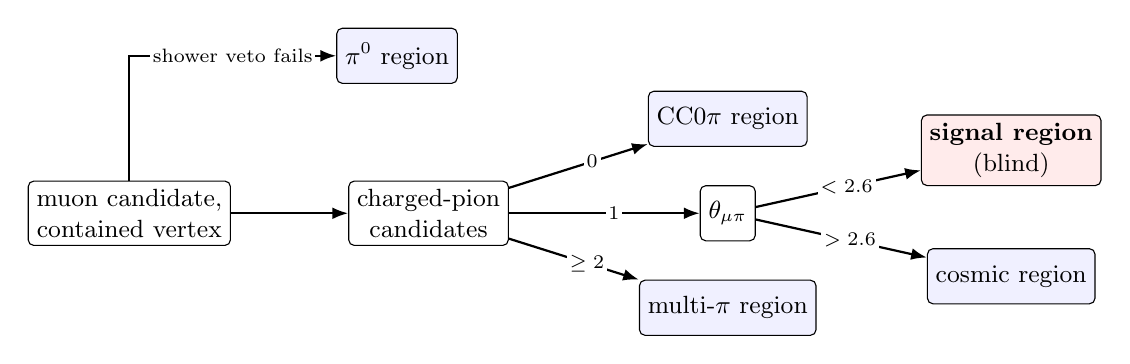
\begin{tikzpicture}[
      font=\small, x=1mm, y=1mm,
      box/.style={draw, rounded corners=2pt, align=center, inner sep=3pt, minimum height=7mm},
      sig/.style={box, fill=red!8},
      cr/.style={box, fill=blue!6},
      ar/.style={-{Latex[length=2mm]}, thick},
      lbl/.style={font=\scriptsize, fill=white, inner sep=1pt}]
    \node[box]  (pre)   at (0,0)    {muon candidate,\\contained vertex};
    \node[cr]   (pi0)   at (34,20)  {$\pi^0$ region};
    \node[box]  (np)    at (38,0)   {charged-pion\\candidates};
    \node[cr]   (cc0)   at (76,12)  {CC$0\pi$ region};
    \node[cr]   (multi) at (76,-12) {multi-$\pi$ region};
    \node[box]  (oa)    at (76,0)   {$\theta_{\mu\pi}$};
    \node[sig]  (sr)    at (112,8)  {\textbf{signal region}\\(blind)};
    \node[cr]   (cos)   at (112,-8) {cosmic region};
    \draw[ar] (pre) -- (np);
    \draw[ar] (pre.north) |- node[lbl, pos=0.75]{shower veto fails} (pi0.west);
    \draw[ar] (np) -- node[lbl, pos=0.6]{$0$} (cc0);
    \draw[ar] (np) -- node[lbl, pos=0.6]{$\geq2$} (multi);
    \draw[ar] (np) -- node[lbl, pos=0.55]{$1$} (oa);
    \draw[ar] (oa) -- node[lbl, pos=0.55]{$<2.6$} (sr);
    \draw[ar] (oa) -- node[lbl, pos=0.55]{$>2.6$} (cos);
  \end{tikzpicture}
  \caption{How the four control regions relate to the signal region. Each is one inverted
    requirement of the signal selection, so no event can be in both: the regions are disjoint from
    the signal region by construction, which is what allows them to be inspected on beam-on data
    while the signal region stays blind.}
  \label{fig:regions}
\end{figure}

\subsection{What the control regions show}
\label{sec:cr_outcome}

The four regions have been opened on beam-on data. They test the background model at reconstruction
level, with the signal region untouched, and the procedure they follow --- the frozen definitions,
the pre-agreed test statistic and the conditions under which a correction may be applied --- is
given in \suppref{Sec.}{sec:request}. Three things come out of them.

\begin{itemize}\itemsep3pt
  \item \textbf{The background model needs no correction.} A joint FHC$+$RHC fit of the background
    class normalisations returns the dominant CC$0\pi$ class at $0.984\pm0.191$, unity within a
    fifth of its own uncertainty (\crref{Sec.}{sec:jointfit}). The measurement keeps its nominal
    background prediction.
  \item \textbf{One run's exposure is wrong, and the cause is identified.} The global test passes
    in every period except FHC Run~1, where every region sits at $0.60$--$0.72$ and a free exposure
    factor fits $0.520\pm0.020$. Two sets of bookkeeping numbers exist for that run --- $2.192\times
    10^{20}$~POT with $5\,748\,692$ triggers without the open trigger, and $3.283\times10^{20}$ with
    $9\,846\,635$ with it --- and every configuration in this analysis assumes the second. The data
    say it is the first. The assumption enters the prediction three ways that all scale with it (the
    neutrino MC through the POT, the beam-off through the gate count, the dirt through the POT), so
    the four combinations can be told apart: assuming the open-trigger pair gives region ratios of
    $0.637$, $0.715$, $0.911$ and $0.595$, while assuming the non-open pair gives $0.970$, $1.090$,
    $1.380$ (on $40$ events) and $0.948$. The two mixed hypotheses leave the beam-off-dominated
    cosmic region at $0.72$--$0.75$, so both numbers are wrong together rather than one of them.

    This does not stay in the control regions. FHC Run~1 is $37\%$ of the assumed FHC exposure, so
    the correction takes FHC from $8.857$ to $7.766\times10^{20}$~POT and would raise the FHC cross
    section by $14.0\%$ and the combined one by $5.8\%$; RHC is untouched, and fake-data closure is
    unaffected because the throws use the same assumed exposure. \textbf{No configuration has been
    changed}: the exposure must be confirmed against the beam bookkeeping before a released
    normalisation moves. This is an unblinding prerequisite (\S\ref{sec:limitations}).
  \item \textbf{The remaining deficit is not signal contamination.} The regions sit $8$--$16\%$
    below prediction. Tightening each region so that it holds less signal --- the CC$0\pi$ region
    goes from $8.7\%$ to $2.1\%$ signal while keeping $58\%$ of its events --- leaves the
    data-to-prediction ratio where it was, $0.84\to0.85$ (\crref{Sec.}{sec:farsb}). Whatever causes
    the deficit does not scale with the signal content of the region.
\end{itemize}

\subsection{Pre-opening validation of the control-region machinery (pseudo-data)}
\label{sec:sidebands}
% =============================================================================

\begin{quote}
\textbf{This subsection is the test that was run before the control regions were opened, and it
is not a test of the background model.} The pseudo-data used here contain only the central-value
neutrino-MC component, so what these ratios validate is the implementation --- the region
definitions, the per-run exposure scaling and the central-value weighting --- on a sample where the
right answer is known by construction. The full-stack variant of
\suppref{Sec.}{sec:cr_fullstack} additionally exercises the bookkeeping path. \textbf{The beam-on
results are in \S\ref{sec:cr_outcome}}, where the regions are compared with the complete
neutrino-MC $+$ beam-off $+$ dirt prediction under the frozen procedure of
\suppref{Sec.}{sec:cr_protocol}.
\end{quote}

Because the analysis is blind, the background model cannot yet be confronted with
beam-on data in the signal region. To exercise it before unblinding, four
signal-depleted control regions (``sidebands'') are defined, each anchored by the
inversion of one nominal signal requirement, with the requirements that the inversion
leaves undefined dropped explicitly (branch-level definitions in
\suppref{Table}{tab:cr_defs}):
\begin{itemize}
  \item \textbf{CC$0\pi$}: the muon selection with no reconstructed charged pion
    (charged-current quasi-elastic / $2p2h$-enriched);
  \item \textbf{multi-$\pi$}: two or more charged pions (deep-inelastic / resonant
    multi-pion);
  \item \textbf{$\pi^0$}: a reconstructed shower present but the $\pi^0$ shower veto
    failed (CC$\,\pi^0$ / NC$\,\pi^0$);
  \item \textbf{cosmic}: the full signal selection with the muon--pion opening angle
    inverted ($\theta_{\mu\pi}>2.6$), enriched in out-of-time cosmic activity.
\end{itemize}
Each region is evaluated with the same per-run POT scaling and CV event weighting
(\S\ref{sec:mc}) used for the measurement. Because the current ``data'' is a Poisson
throw of the neutrino Monte Carlo central value only (it contains no EXT or dirt
component), the meaningful closure quantity here is the ratio of the pseudo-data to the
CV-weighted \emph{neutrino} MC, $N_\mathrm{data}/N_{\nu\mathrm{MC}}$; the EXT and dirt
yields are shown for scale but enter the background-model test only once real beam-on
data are available. Table~\ref{tab:sidebands} summarises the four regions for the three
beam configurations.

\begin{table}[H]
  \centering
  \caption{Background-control sidebands. ``Signal fraction'' is the signal
    contamination of the (CV-weighted neutrino) MC in the region; all four are strongly
    signal-depleted. $N_\mathrm{data}/N_{\nu\mathrm{MC}}$ is the pseudo-data to
    neutrino-MC ratio: the high-statistics regions (CC$0\pi$, $\pi^0$) close to unity
    across FHC/RHC/combined, validating the per-run weighting and POT-scaling machinery;
    the low-statistics regions (multi-$\pi$, cosmic) scatter within Poisson expectation
    ($\sqrt{N}\!\approx\!6$--$10\%$). The background-model test against the full stack
    (with EXT and dirt) is performed at control-region unblinding with beam-on data.}
  \label{tab:sidebands}
  \begin{tabular}{llccc}
    \toprule
    & Signal frac.\ & \multicolumn{3}{c}{$N_\mathrm{data}/N_{\nu\mathrm{MC}}$} \\
    \cmidrule(lr){3-5}
    Sideband & (of $\nu$MC) & FHC & RHC & Combined \\
    \midrule
    CC$0\pi$      & $\sim10\%$ & $1.00$ & $0.99$ & $1.00$ \\
    multi-$\pi$   & $\sim23\%$ & $1.01$ & $1.10$ & $1.06$ \\
    $\pi^0$       & $\sim10\%$ & $1.00$ & $1.01$ & $1.00$ \\
    cosmic        & $\sim8\%$ & $1.09$ & $0.99$ & $1.04$ \\
    \bottomrule
  \end{tabular}
\end{table}

\paragraph{Yields and composition.}
Table~\ref{tab:sideband_yields} gives the full breakdown for the three configurations. The
regions differ enormously in size and in what they are sensitive to, which is what makes
them complementary rather than redundant:

\begin{itemize}
  \item \textbf{CC$0\pi$} is by far the largest ($\sim\!12$k pseudo-data events per beam,
    $\sim\!24$k combined). Its neutrino component is dominated by the quasi-elastic and
    $2p2h$ modes that feed the signal region only through pion \emph{absorption} in the
    final state. It is therefore the natural handle on the FSI model that converts
    CC$\,1\pi^{\pm}$ into CC$0\pi$ and vice versa; the largest single migration path
    into and out of the signal definition (\S\ref{sec:signal}).
  \item \textbf{$\pi^0$} is the second largest ($6.6$--$14.8$k). It is enriched in
    CC/NC$\,\pi^0$ events, whose showers are precisely what the shower veto (Cut~8) is
    designed to remove; it therefore tests the veto efficiency and the $\pi^0$ production
    normalisation together. These are the events that leak into the signal region when a
    photon is missed.
  \item \textbf{multi-$\pi$} is small ($125$--$300$ events) but has the highest signal
    contamination of the four ($\sim\!23\%$), because a true multi-pion event with one
    pion lost is exactly the wrong-topology background the selection fights. Its size is
    what limits its constraining power at present.
  \item \textbf{cosmic} is the region with by far the largest beam-off (EXT) share of
    the prediction: $53$ EXT against $75$ neutrino-MC events for FHC, a ratio of $0.7$,
    against $0.1$ in CC$0\pi$ (with the per-run beam-off treatment of \S\ref{sec:mc}). It
    is the region that tests the beam-off normalisation and shape,
    and the one whose interpretation changes most at unblinding, since the current
    pseudo-data contain no EXT component at all. Its beam-off purity is only $41\%$
    (FHC; $34\%$ RHC), so under the target-purity requirement of \suppref{Sec.}{sec:cr_protocol}
    it is diagnostic: it cannot by itself produce a fitted EXT normalisation correction,
    only an additional uncertainty.
\end{itemize}

\paragraph{What the present numbers do and do not show.}
With Poisson-thrown neutrino-MC pseudo-data, the ratios of Table~\ref{tab:sidebands}
test the \emph{machinery}, per-run POT scaling, CV weighting, the selection logic in
each inverted region, and not the background model. That test passes: the two
high-statistics regions sit at $N_\mathrm{data}/N_{\nu\mathrm{MC}}=0.99$--$1.01$ in all
three configurations, which checks that the per-run scaling is applied identically on
the throw and the prediction paths, not the normalisation itself. The apparent deviations in the
small regions are statistical: with $82$ cosmic-sideband events for FHC, a $\sqrt{N}$
fluctuation is $11\%$, so the observed $1.09$, and the RHC multi-$\pi$ $1.10$ (on $175$
events, $8\%$), are within about one standard deviation.

\paragraph{What the regions could deliver.}
These yields set the statistical precision that was available when the regions were opened, and
the estimates were made beforehand; what they actually showed is \S\ref{sec:cr_outcome}. The
combined CC$0\pi$ and $\pi^0$ samples have $0.6\%$ and $0.8\%$ \emph{raw data
statistical} precision. Their effective constraint on the signal-region background is
weaker and depends on the correlated transfer uncertainty
(\suppref{Sec.}{sec:cr_transfer}): the transfer factors are small ($0.03$ and $0.02$) but the
transfer from a CC$0\pi$ event to a selected CC$1\pi$ topology is itself model
dependent, so the achievable constraint is set by the cross-section and detector terms
of that transfer rather than by the sample size. The cosmic region
would constrain the EXT normalisation only to $\sim\!50\%$ ($94$ EXT events among
$\sim\!250$ combined: $\sqrt{257}=16$ events of data statistics against the $32\%$
prediction systematic on the $145$ neutrino-MC events in the region, $\pm46$; $\sim\!17\%$
from data statistics alone);
with the beam-off at $1.9\%$ of the signal-region sample that is adequate. No
uncertainty is currently assigned to the gate ratios themselves or to the Run-1 sample
standing in for Run~2 ($14\%$ of the FHC and $23\%$ of the RHC exposure); both are
listed in \S\ref{sec:limitations}. The multi-$\pi$ region, at $\sim\!300$
combined events, gives $\sim\!6\%$, useful as a cross-check but not competitive with
the others. The procedure followed was to open the control regions first, use them to test --- and where
item~4 of \suppref{Sec.}{sec:cr_protocol} permits, to correct --- the normalisation of the dominant
background classes, and only then to open the signal region. The signal region remains blinded.

\begin{table}[H]
  \centering
  \caption{Sideband yields at full exposure. ``Signal'' is the signal contamination of the
    neutrino MC (events satisfying the inclusive signal definition of \S\ref{sec:signal};
    all yields and the pseudo-data throw apply the safe-weight rule of
    Eq.~\eqref{eq:safeweight}), ``$\nu$ bkg'' the remaining neutrino MC, EXT the per-run beam-off
    (cosmic) samples scaled by the run gate ratios (\S\ref{sec:mc}), and dirt the
    out-of-cryostat overlay. The pseudo-data
    column is a Poisson throw of the neutrino MC only, so it should be compared with
    Signal $+$ $\nu$ bkg; EXT and dirt are listed for scale and enter the comparison only
    with real beam-on data.}
  \label{tab:sideband_yields}
  \small
  \begin{tabular}{llrrrrrc}
    \toprule
    Beam & Sideband & Pseudo-data & Signal & $\nu$ bkg & EXT & Dirt & Sig.\ frac. \\
    \midrule
    FHC & CC$0\pi$ & $12\,181$ & $1\,124$ & $11\,068$ & $1\,358$ & $56$ & $9.2\%$ \\
    FHC & multi-$\pi$ & $125$ & $30$ & $94$ & $7.2$ & $0.1$ & $24.0\%$ \\
    FHC & $\pi^0$ & $6\,628$ & $662$ & $5\,985$ & $778$ & $12$ & $10.0\%$ \\
    FHC & cosmic & $82$ & $6.0$ & $69$ & $53$ & $2.2$ & $7.9\%$ \\
    \midrule
    RHC & CC$0\pi$ & $12\,590$ & $1\,206$ & $11\,452$ & $1\,214$ & $43$ & $9.5\%$ \\
    RHC & multi-$\pi$ & $175$ & $35$ & $124$ & $5.9$ & $0.1$ & $22.0\%$ \\
    RHC & $\pi^0$ & $8\,176$ & $780$ & $7\,300$ & $678$ & $9.1$ & $9.6\%$ \\
    RHC & cosmic & $81$ & $6.4$ & $75$ & $42$ & $1.7$ & $7.9\%$ \\
    \midrule
    Comb & CC$0\pi$ & $24\,771$ & $2\,329$ & $22\,520$ & $2\,572$ & $99$ & $9.4\%$ \\
    Comb & multi-$\pi$ & $300$ & $65$ & $218$ & $13$ & $0.2$ & $22.9\%$ \\
    Comb & $\pi^0$ & $14\,804$ & $1\,441$ & $13\,285$ & $1\,455$ & $21$ & $9.8\%$ \\
    Comb & cosmic & $163$ & $12$ & $145$ & $94$ & $3.9$ & $7.9\%$ \\
    \bottomrule
  \end{tabular}
\end{table}

% =============================================================================

\section{Secondary scope: proton-tagged subsample (hadronic invariant mass and
  transverse kinematic imbalance)}
\label{sec:wtki}

\begin{quote}
\textbf{Scope note.}  This section is secondary scope. Its extractions carry the complete
configured covariance, detector variations included, with detector terms of $10.5\%$ to
$108.5\%$ (median $33.0\%$) against $15.6\%$--$35.0\%$ for the inclusive results: the
same order, as expected for the same detector, except for the six-bin observables on the
sparsest samples, where the unfolding amplifies them. The additional-smearing and
covariance matrices are released with the rest (Sec.~\ref{sec:ac_rowsums}). What makes
the scope secondary is a binning limitation that no systematic treatment addresses: the
differential $W_{\pi p}$ shape is withdrawn, because at this exposure no binning
satisfies both the migration and the statistics requirement, so the proton-tagged sample
supports an integrated cross section, not a resonance-shape measurement; and the
proton-mistag background has no dedicated control region yet
(\suppref{Sec.}{sec:cr_1p_scope}). See Sec.~\ref{sec:status_matrix}.
\end{quote}

\begin{quote}
\textbf{On the six-bin $W_{\pi p}$ material below.}  Any six-bin $W_{\pi p}$ distribution in this
section is \emph{diagnostic}: it shows why the shape is not measurable and is not a result. The
differential $W_{\pi p}$ shape is withdrawn (Appendix~\ref{app:withdrawn}); the proton-tagged
deliverable is the integrated cross section.
\end{quote}
% =============================================================================

Requiring an identified proton in the final state, in addition to the muon and charged
pion, reconstructs the full visible hadronic system and opens two classes of observable
inaccessible to the inclusive $\mathrm{CC}\,1\mu1\pi Xp$ measurement: the \emph{hadronic
invariant mass}, which probes the $\Delta(1232)$ and higher resonances directly, and the
\emph{transverse kinematic imbalance} (TKI) between the muon and the hadronic system,
which is sensitive to Fermi motion and final-state interactions. The proton-tagged
selection, its signal definition and its performance are given in
\S\ref{sec:selection_1p}; in brief, it adds a leading-proton identification to the
inclusive selection, at an efficiency of $11.4\%$ and a purity of $50$--$52\%$, and
trades signal statistics for a fully reconstructed hadronic final state.

\subsection{Extracted cross sections}

Eleven observables are extracted in the proton-tagged subsample; ten are carried as
\emph{secondary validation products}, with their covariances but not proposed for
approval in this review (the binning validation of $W_\mathrm{had}$ and the dedicated
control region are incomplete, \S\ref{sec:limitations}); the eleventh, the
differential $W_{\pi p}$ shape, is withdrawn (its files are in the release for
completeness, flagged as such in \texttt{index\_extractions.tsv}), and the robust
proton-tagged deliverable proposed as a headline is the one-bin total cross section
(Table~\ref{tab:cutcount}). Two further observables, the proton angles $\theta_p$ and
$\theta_{\pi p}$ (\S\ref{sec:wtki_ang}), were added afterwards and are proposed as secondary scope;
this is the arithmetic behind the twelve rows of Tables~\ref{tab:wtki_fhc}--\ref{tab:wtki_comb},
which are the ten validation products plus those two, the withdrawn $W_{\pi p}$ shape appearing
only in the technical supplement. The ten are: the five hadronic-mass and
transverse-kinematic-imbalance (W/TKI) variables specific to this selection
($W_\mathrm{had}$ and the four TKI observables), plus the five muon/pion kinematic observables of the inclusive analysis
($p_\mu$, $p_\pi$, $\cos\theta_\mu$, $\cos\theta_\pi$, $\theta_{\mu\pi}$) re-measured on
the proton-tagged phase space so that the two selections share a common set of
kinematic distributions. The two hadronic-mass variables are the
\emph{directly measured} $\pi p$ invariant mass,
$W_{\pi p}=\big[(E_\pi+E_p)^2-(\vec p_\pi+\vec p_p)^2\big]^{1/2}$, which makes no
assumption on the neutrino direction, and the \emph{calorimetric} hadronic mass
$W_\mathrm{had}=\big[m_p^2+2m_p(E_\mathrm{cal}-E_\mu)-Q^2\big]^{1/2}$ built from the
reconstructed calorimetric energy. The four TKI observables; the transverse-momentum
imbalance $\delta p_T$, its two angles $\delta\alpha_T$ and $\delta\phi_T$~\cite{lu_tki}, and the
STV-inferred nucleon-momentum proxy $p_n$~\cite{furmanski_pn} (an approximation, see below), are computed
from the muon versus the summed $(\pi+p)$ hadronic system using the framework STV tool.
Proton momenta are obtained from
the proton-hypothesis range-based kinetic energy. $W_\mathrm{had}$ is measured
in six equal-population bins ($W_{\pi p}$ was binned the same way for the diagnostic
study in the supplement); the four TKI variables use the coarsened two-bin scheme
adopted after the finer binning was found to sit inside the resolution
(\suppref{Sec.}{sec:w_binning}); the reverse-horn-current sample uses the same binning
as FHC. The five inherited kinematic observables use the inclusive-analysis binning (two to seven bins; the proton-tagged
$\cos\theta_\pi$ keeps the former four-bin inclusive edges). All bin edges are set
from the validated true-signal distributions (\suppref{Table}{tab:wtki_binning}).

\paragraph{Reconstruction.} Every observable is built from the three candidate tracks --- muon,
charged pion, proton --- using reconstructed quantities only: range or multiple-scattering
momentum for the muon, range momentum for the pion, calorimetric kinetic energy for the proton,
and the track directions, all in the beam frame. The formulae and the conventions of the
transverse-imbalance tool are given in \suppref{Sec.}{sec:wtki_reco}.

The pipeline is validated end-to-end on FHC with a fake-data closure: the Poisson-thrown
central-value pseudo-data are unfolded with the same Wiener-SVD procedure
(\S\ref{sec:unfolding}) and compared to the $A_C$-smeared truth. Table~\ref{tab:wtki_fhc}
shows the result. The bin-by-bin $\chi^2/\mathrm{ndf}$ is well below unity for every
observable, confirming the unfolded pseudo-data are statistically consistent with truth
and that the response, background subtraction and normalisation are self-consistent. The
integrated-cross-section ratios ($0.96$--$1.08$) are ratios to the $A_C$-smeared truth,
so they measure the statistical scatter of this throw (and any bias), not the $A_C$
suppression, which is common to numerator and denominator; the largest departures are
in $\cos\theta_\mu$ and $p_\mu$. The
systematic treatment here includes the flux, cross-section, reinteraction and
detector-variation terms.

The reverse-horn-current measurement is complete at the same binning
(Table~\ref{tab:wtki_rhc}). All ten proton-tagged validation products close positive in RHC, with
$\sigma_\mathrm{int}$ in $0.31$--$0.44\times10^{-38}$~cm$^2$/Ar against $0.39$--$0.50$
for FHC; these are $A_C$-suppressed integrals with different $A_C$ per configuration, so
their ratio is not the RHC/FHC ratio (that is $0.860$ from the one-bin totals,
Table~\ref{tab:cutcount}). The closure gives $\chi^2/\mathrm{ndf}\lesssim1$ for almost
every observable.

The two families of processed files store the simulated exposure under different conventions;
the run-by-run normalisation used here is correct under both (\suppref{Sec.}{sec:wtki_reco}).

The combined-sample measurement is complete on the same binning, is included in the
results tables and the data release, and covers all ten combined proton-tagged validation products.

\begin{table}[H]
  \centering
  \caption{FHC fake-data closure for the twelve proton-tagged observables.
    $\sigma_\mathrm{int}$ is the integrated (unfolded) cross section over the
    measured phase space ($10^{-38}$~cm$^2$/Ar); ``unf./truth'' is the ratio of integrals;
    $\chi^2$ is the bin-by-bin comparison of unfolded pseudo-data to $A_C$-smeared truth
    (ndf = number of bins). The upper block is the five released W/TKI observables;
    $W_\mathrm{had}$ is at six bins, while the four TKI variables use the coarsened two-bin
    scheme adopted after the finer binning was found to sit inside the resolution; the
    six-bin $W_{\pi p}$ closure rows are diagnostic only and are given in the technical
    supplement (\suppref{Sec.}{sec:w_binning});
    the lower block is the five kinematic observables inherited from the inclusive
    analysis. The small $\chi^2/\mathrm{ndf}$ validates the chain. The integral ratios compare
    the unfolded result with the $A_C$-smeared truth, so departures from unity reflect
    the statistical realisation of the throw and any residual extraction bias; they do
    not measure the suppression introduced by $A_C$. The third block ($^{\dagger}$) is the two angular observables proposed as secondary scope (\S\ref{sec:wtki_ang}).}
  \label{tab:wtki_fhc}
  \begin{tabular}{lccc}
\toprule
Observable & $\sigma_\mathrm{int}$ & unf./truth & $\chi^2/\mathrm{ndf}$ \\
\midrule
      $W_\mathrm{had}$   & $0.389$ & $1.00$ & $0.88/6$ \\
      $\delta p_T$       & $0.461$ & $0.98$ & $0.01/2$ \\
      $\delta\alpha_T$   & $0.485$ & $0.96$ & $0.02/2$ \\
      $\delta\phi_T$     & $0.474$ & $0.99$ & $0.11/2$ \\
      $p_n$              & $0.490$ & $0.98$ & $0.06/2$ \\
      \midrule
      $p_\mu$            & $0.496$ & $1.04$ & $1.89/7$ \\
      $p_\pi$            & $0.498$ & $0.98$ & $0.01/2$ \\
      $\cos\theta_\mu$   & $0.445$ & $1.08$ & $0.98/5$ \\
      $\cos\theta_\pi$   & $0.394$ & $0.99$ & $0.30/4$ \\
      $\theta_{\mu\pi}$  & $0.469$ & $1.02$ & $0.50/5$ \\
      \midrule
      $\theta_p$$^{\dagger}$         & $0.532$ & $0.98$ & $1.92/4$ \\
      $\theta_{\pi p}$$^{\dagger}$      & $0.456$ & $0.99$ & $0.16/3$ \\
\bottomrule
\end{tabular}
\end{table}


Figure~\ref{fig:dsigma_ccpi1p_fhc} shows the five released FHC W/TKI differential cross
sections ($W_\mathrm{had}$ and the four TKI observables), overlaid with all four generator
predictions; the withdrawn six-bin $W_{\pi p}$ distribution is deliberately not shown
here, and its diagnostic closure and generator curves are in the technical supplement
(\suppref{Sec.}{sec:w_binning}). The generator
W/TKI predictions were regenerated at this binning (GENIE and GiBUU natively, NuWro and
NEUT from their event vectors inside the SL7 container). All curves, data, tune and
generators, are $A_C$-smeared, so the comparison is made consistently in the
measurement space (\suppref{Sec.}{sec:acwtki}). The predictions are built at truth level from each
generator's event-level final state, GENIE gst events, GiBUU final-event records,
and the NuWro and NEUT event vectors reprocessed in their respective SL7-container
environments, by applying the inclusive signal plus a leading true proton above
$0.3$~GeV/$c$ and evaluating the six observables with the same formulas as the selection
(\suppref{Sec.}{sec:wtki_reco}), then combining the $\nu_\mu$ and $\bar\nu_\mu$ samples over the
FHC flux to a per-argon cross section. The four generators span a factor of $\sim1.6$ in
the integrated proton-tagged cross section, GENIE lowest ($0.50$), then NuWro
($0.65$), GiBUU ($0.74$) and NEUT highest ($0.78\times10^{-38}$~cm$^2$/Ar), bracketing
the injected tune (proton-tagged one-bin total, Table~\ref{tab:cutcount}). In
the released two-bin TKI scheme the differences between generators are almost entirely
normalisation: their shapes, and that of the tune, agree with the unfolded points within
the uncertainties in every panel, so the present exposure does not discriminate between
the generators' treatments of Fermi motion and final-state interactions. Data and
predictions are both computed about the beam axis (\S\ref{sec:beamdir}); a comparison in
which one side used the detector $z$ axis would show apparent shape disagreements of a
factor of several, which is why the frame is stated with every transverse quantity.

\begin{table}[H]
  \centering
  \caption{As Table~\ref{tab:wtki_fhc}, for RHC.}
  \label{tab:wtki_rhc}
  \begin{tabular}{lccc}
\toprule
Observable & $\sigma_\mathrm{int}$ & unf./truth & $\chi^2/\mathrm{ndf}$ \\
\midrule
      $W_\mathrm{had}$   & $0.314$ & $0.96$ & $0.69/6$ \\
      $\delta p_T$       & $0.418$ & $1.10$ & $0.52/2$ \\
      $\delta\alpha_T$   & $0.438$ & $1.08$ & $0.19/2$ \\
      $\delta\phi_T$     & $0.389$ & $1.02$ & $0.10/2$ \\
      $p_n$              & $0.391$ & $1.00$ & $1.06/2$ \\
      \midrule
      $p_\mu$            & $0.380$ & $1.09$ & $3.80/7$ \\
      $p_\pi$            & $0.429$ & $1.09$ & $1.21/2$ \\
      $\cos\theta_\mu$   & $0.392$ & $1.11$ & $0.84/5$ \\
      $\cos\theta_\pi$   & $0.365$ & $1.10$ & $6.01/4$ \\
      $\theta_{\mu\pi}$  & $0.367$ & $0.96$ & $0.14/5$ \\
      \midrule
      $\theta_p$$^{\dagger}$         & $0.391$ & $0.99$ & $0.04/4$ \\
      $\theta_{\pi p}$$^{\dagger}$      & $0.378$ & $1.02$ & $0.12/3$ \\
\bottomrule
\end{tabular}
\end{table}

\begin{table}[H]
  \centering
  \caption{As Table~\ref{tab:wtki_fhc}, for the combined configuration. The combined result is an independent extraction with its own response and $A_C$, not an average of FHC and RHC, so it need not lie between them.}
  \label{tab:wtki_comb}
  \begin{tabular}{lccc}
\toprule
Observable & $\sigma_\mathrm{int}$ & unf./truth & $\chi^2/\mathrm{ndf}$ \\
\midrule
      $W_\mathrm{had}$   & $0.345$ & $0.99$ & $0.85/6$ \\
      $\delta p_T$       & $0.540$ & $1.09$ & $0.17/2$ \\
      $\delta\alpha_T$   & $0.459$ & $1.01$ & $0.02/2$ \\
      $\delta\phi_T$     & $0.503$ & $1.09$ & $0.24/2$ \\
      $p_n$              & $0.449$ & $1.02$ & $0.85/2$ \\
      \midrule
      $p_\mu$            & $0.437$ & $1.03$ & $1.53/7$ \\
      $p_\pi$            & $0.462$ & $1.03$ & $0.40/2$ \\
      $\cos\theta_\mu$   & $0.410$ & $1.06$ & $1.52/5$ \\
      $\cos\theta_\pi$   & $0.382$ & $1.02$ & $3.40/4$ \\
      $\theta_{\mu\pi}$  & $0.445$ & $1.04$ & $0.26/5$ \\
      \midrule
      $\theta_p$$^{\dagger}$         & $0.485$ & $1.01$ & $0.67/4$ \\
      $\theta_{\pi p}$$^{\dagger}$      & $0.413$ & $1.01$ & $0.06/3$ \\
\bottomrule
\end{tabular}
\end{table}

\begin{figure}[H]
  \centering
  \blindfig[\textwidth]{dsigma_ccpi1p_noW_FHC5}
  \caption{Proton-tagged released differential cross sections for
    FHC: the calorimetric hadronic mass
    $W_\mathrm{had}$ and the four transverse-kinematic-imbalance observables
    $\delta p_T$, $\delta\alpha_T$, $\delta\phi_T$ and $p_n$ (the withdrawn $W_{\pi p}$
    shape is not shown; see the technical supplement). Unfolded fake data
    (black points) are compared to the $A_C$-smeared fake-data truth (grey dashed), the
    MicroBooNE tune (black), and the GENIE (blue), GiBUU (green), NEUT (purple) and
    NuWro (orange) predictions built for the same proton-tagged phase space.
    $\delta\alpha_T$ rises toward $180^\circ$, the
    signature of final-state interactions.}
  \label{fig:dsigma_ccpi1p_fhc}
\end{figure}

\begin{figure}[H]
  \centering
  \blindfig[\textwidth]{dsigma_ccpi1p_noW_RHCFULL}
  \caption{The same five proton-tagged observables for RHC. Curves and points as in
    Fig.~\ref{fig:dsigma_ccpi1p_fhc}.}
  \label{fig:dsigma_ccpi1p_rhc}
\end{figure}

\begin{figure}[H]
  \centering
  \blindfig[\textwidth]{dsigma_ccpi1p_noW_COMB}
  \caption{The same five proton-tagged observables for the combined configuration. Curves and
    points as in Fig.~\ref{fig:dsigma_ccpi1p_fhc}.}
  \label{fig:dsigma_ccpi1p_comb}
\end{figure}


With all three configurations in hand, the combined $\sigma_\mathrm{int}$ lies between the
FHC and RHC values for eight of the ten proton-tagged validation products; $\delta p_T$ ($0.540$
against $0.461$ and $0.418$) and $\delta\phi_T$ ($0.503$ against $0.474$ and $0.389$)
lie above both, by amounts well inside their $\sim\!30\%$ uncertainties.

That is not a defect: the combined measurement is \emph{not} required to lie between the two
single-mode ones.  It is an independent extraction with its own response matrix, its own
regularisation and its own $A_C$, not a fluence-weighted average, so excursions at the
few-per-cent level would have been unremarkable against a $\sim\!30\%$ systematic
uncertainty.

The spread across observables within a configuration, $0.35$ to $0.54$ for the combined
set, is likewise not a physics spread but the residual of the additional smearing
discussed in the next section: each observable's $A_C$ rescales the integral by a different
factor, so the ten numbers are not ten independent measurements of the same quantity.

\subsection{What the proton candidate is}
\label{sec:prmatch}

Every proton-tagged observable is built on the reconstructed proton candidate, while the truth-level
definitions use the leading true proton. On selected signal events the candidate is the leading true
proton $81.7\%$ of the time, some true proton $87.4\%$, and not a proton at all $12.6\%$
($10\,105$ events).

What that costs was measured for the two angular observables, and the answer depends on which
question is asked. A correct pick reconstructs the angle tightly (interquartile range $0.073$~rad in
$\theta_p$, $0.124$~rad in $\theta_{\pi p}$); a wrong pick does not smear the angle, it randomises it
($1.0$--$1.4$~rad, three quarters of those events beyond $0.3$~rad). Averaged over everything the
candidate widens the \emph{core} resolution by only a quarter to a third, which understates it badly,
because a binned measurement is not limited by its core. Residuals beyond $0.3$~rad occur in $18.9\%$
of $\theta_p$ events and \emph{$74\%$ of those are wrong picks} ($\theta_{\pi p}$: $25.9\%$ and
$51\%$). Candidate purity is therefore the dominant source of bin-to-bin migration in $\theta_p$,
which is why its migration diagonal sits at the criterion and its RHC response is rank-deficient.

The same $18\%$ wrong-pick rate applies to $W_{\pi p}$, $W_\mathrm{had}$ and the TKI observables,
which use the same candidate; the migration attribution above was measured for the angles only. The
control region that would constrain this is the multi-$\pi$ sideband, which is already open:
\texttt{pion\_number} is defined by the same PID cut that picks the proton, so an otherwise-signal
event whose proton fails it has two pion candidates and lands there. It constrains the
proton~$\to$~pion direction rather than the pion~$\to$~proton one that produces the $12.6\%$, and it
is the most signal-contaminated of the four regions, so a region inverting the proton PID at exactly
one pion candidate is what would separate them.

\subsection{Proton angular observables: \texorpdfstring{$\theta_p$}{theta p} and
  \texorpdfstring{$\theta_{\pi p}$}{theta pi p}}
\label{sec:wtki_ang}

Two angular observables of the proton-tagged sample are proposed as secondary scope. Like every
other number in this note they are fake data. Both use the leading proton candidate:
\[
  \theta_p=\arccos\!\big(\hat p_p\cdot\hat\nu\big), \qquad
  \theta_{\pi p}=\arccos\!\big(\hat p_\pi\cdot\hat p_p\big),
\]
with $\hat\nu$ the beam-frame neutrino direction of \S\ref{sec:beamdir} --- the same convention as
every other angle here --- while $\theta_{\pi p}$ is an angle between two reconstructed tracks and
so needs no beam direction at all, which makes it the one angular observable in this analysis that
is insensitive to the beam-frame convention. $\theta_p$ is available from the stored proton
direction; $\theta_{\pi p}$ required the proton-tagged tree to be reprocessed to write
\texttt{pi\_pr\_opening\_angle\_\{reco,true\}}, checked to leave every existing branch unchanged.

They measure something the released set does not. The five W/TKI observables are built from the
muon against the \emph{summed} hadronic system, so they are insensitive to how that system shares
its momentum between pion and proton; $\theta_{\pi p}$ is exactly that sharing. $\theta_p$ is the
proton direction alone, where the released set has only the derived quantities.

Both unfold well (Tables~\ref{tab:wtki_fhc}--\ref{tab:wtki_comb}). $\theta_{\pi p}$ is the
best-conditioned observable of the proton-tagged programme, $s_{\min}/s_1=0.30$--$0.48$ against
$0.27/0.24$ for the released $\cos\theta_\pi$, at the price of a last bin whose total uncertainty
reaches $93\%$ (FHC) and $187\%$ (RHC). $\theta_p$ conditions at $0.383$ (FHC) and $0.408$
(combined) but is rank-deficient in RHC ($0.001$), so it is proposed for FHC and the combined
configuration only; coarsening the RHC binning was tried and does not rescue it. Its edges are
derived on the RHC chain rather than the FHC one: at the same four bins they condition three times
better in both usable configurations. Both distributions are strongly forward peaked, and the
generators differ mainly in normalisation rather than shape, so these observables discriminate
through the integral. The study behind all of this --- binning, generator predictions, the
$0.50$-criterion screen and the two-dimensional programme --- is a separate note.

\begin{figure}[H]
  \centering
  \blindfig[\textwidth]{newobs_xsec}
  \caption{The two proton angular observables in all three configurations: $\theta_p$ (top row) and
    $\theta_{\pi p}$ (bottom row), for FHC, RHC and the combined exposure. Points are the unfolded
    fake data with the total uncertainty, the grey histogram is the $A_C$-smeared fake-data truth,
    and the four coloured histograms are the generator predictions; integrated cross sections are
    given in the legends. The RHC $\theta_p$ panel is shown for completeness only: its response is
    rank-deficient and its shape is not a measurement.}
  \label{fig:newobs_xsec}
\end{figure}

\subsection{Two-dimensional cross sections (proposed)}
\label{sec:2d}

Eight two-dimensional pairs were screened and extracted in all three configurations. The framework
needed no new unfolding machinery --- a two-dimensional binning is a flat list of analysis bins
ordered slice by slice --- and the integrated normalisation of the two-dimensional chain agrees with
the released one-bin total to a median of $0.7\%$ once each is compared with its own $A_C$-smeared
truth. Two pairs are worth proposing, both in the combined configuration only:
$\theta_p\times\delta p_T$ ($s_{\min}/s_1=0.617$) and $\cos\theta_\pi\times\cos\theta_\mu$
($0.563$). Combining the beam modes roughly doubles their conditioning ($0.46\to0.62$,
$0.25\to0.56$), which is the clearest benefit the joint exposure delivers anywhere in this analysis,
and it comes from statistics and the shared flux rather than from any $\nu/\bar\nu$ separation.
Everything built on $W_{\pi p}$ is unusable, as its $39\%$ leakage between outer bins predicted.

One pair is worth recording as a caution. $\theta_{\pi p}\times W_{\pi p}$ conditions at $0.560$,
as well as the two usable pairs, and its extraction is still worthless: a $58\%$ data-statistical
term, per-bin uncertainties to $545\%$ and a closure ratio of $-0.40$. Conditioning bounds how much
of the response can be inverted and says nothing about how much data survives in the inverted
directions; the two have to be read together, here and everywhere else in this note.

\begin{table}[H]
  \centering
  \caption{The eight two-dimensional pairs (inner $\times$ outer), ordered by the conditioning of
    $A_C$ in the combined configuration. The last three columns are the combined configuration
    only: the bin-averaged data-statistical term, the range of the per-bin total uncertainty and the
    range of the closure ratio against the $A_C$-smeared truth. Fake data.}
  \label{tab:2dextract}
  \small
  \begin{tabular}{lcccccc}
    \toprule
    & \multicolumn{3}{c}{$s_{\min}/s_1$} & \multicolumn{3}{c}{combined configuration} \\
    \cmidrule(lr){2-4}\cmidrule(lr){5-7}
    Pair & FHC & RHC & COMB & data stat. & unc.\ [\%] & closure \\
    \midrule
    $\theta_p\times\delta p_T$ & $0.455$ & $0.332$ & $\mathbf{0.617}$ & $13.7\%$ & $31$--$88$ & $0.82$--$1.25$ \\
    $\cos\theta_\pi\times\cos\theta_\mu$ & $0.245$ & $0.315$ & $\mathbf{0.563}$ & $14.8\%$ & $32$--$62$ & $0.93$--$1.17$ \\
    $\theta_{\pi p}\times W_{\pi p}$ & $0.403$ & $0.214$ & $0.560$ & $57.7\%$ & $43$--$545$ & $-0.40$--$1.10$ \\
    $\cos\theta_\pi\times\theta_{\mu\pi}$ & $0.027$ & $0.133$ & $0.169$ & $22.2\%$ & $28$--$94$ & $0.91$--$1.37$ \\
    $\cos\theta_\mu\times p_\mu$ & $0.002$ & $0.261$ & $0.110$ & $8.9\%$ & $33$--$57$ & $0.97$--$0.99$ \\
    $\theta_p\times W_{\pi p}$ & $0.008$ & $0.152$ & $0.105$ & $111.7\%$ & $36$--$291$ & $0.39$--$1.22$ \\
    $\cos\theta_\pi\times p_\pi$ & $0.023$ & $0.158$ & $0.052$ & $12.9\%$ & $32$--$58$ & $0.96$--$1.14$ \\
    $\theta_{\pi p}\times\delta p_T$ & $0.024$ & $0.035$ & $0.028$ & $10.7\%$ & $28$--$50$ & $0.93$--$1.08$ \\
    \bottomrule
  \end{tabular}
\end{table}

Two entries in that table are worth reading against each other. $\cos\theta_\mu\times p_\mu$
screened best of the eight on the migration diagonal ($0.70/0.68$) and is rank-deficient in FHC
($0.002$); $\theta_p\times\delta p_T$ screened worst of the proton-tagged pairs and conditions best
of all. The diagonal is a necessary condition, not a sufficient one, and the regularised response is
what decides --- the same lesson the one-dimensional binning study returns
(Appendix~\ref{app:altbinning}).

Figures~\ref{fig:2dslices} and~\ref{fig:2dmap} show the two usable pairs. The slice form is how a
double-differential result is normally published and how the generators are compared; the map is the
same numbers, and shows at a glance where the measurement has support. Each slice panel carries its
own vertical scale, because the outer bins differ by an order of magnitude, and the maps are drawn
on equal-size cells labelled by their ranges for the same reason.

\begin{figure}[H]
  \centering
  \blindfig[0.66\textwidth]{bkgfit/xsec2d_thetap_dpt_COMB_slices}\\[6pt]
  \blindfig[0.98\textwidth]{bkgfit/xsec2d_costhpi_costhmu_COMB_slices}
  \caption{The two proposed two-dimensional measurements as slices in the outer variable, combined
    configuration: $\theta_p\times\delta p_T$ (top) and $\cos\theta_\pi\times\cos\theta_\mu$
    (bottom). Points are the unfolded fake data with the total uncertainty, the grey histogram is
    the $A_C$-smeared fake-data truth and the four coloured histograms are the generator
    predictions.}
  \label{fig:2dslices}
\end{figure}

\begin{figure}[H]
  \centering
  \blindfig[0.82\textwidth]{bkgfit/xsec2d_thetap_dpt_COMB_map}\\[6pt]
  \blindfig[0.90\textwidth]{bkgfit/xsec2d_costhpi_costhmu_COMB_map}
  \caption{The same two measurements as maps: $\mathrm{d}^2\sigma/\mathrm{d}X\,\mathrm{d}Y$ per cell
    with its total uncertainty (left) and the ratio to the $A_C$-smeared truth (right), for
    $\theta_p\times\delta p_T$ (top) and $\cos\theta_\pi\times\cos\theta_\mu$ (bottom). Cells are
    equal-size and labelled by their ranges; the colour scale is the one used for the
    matrix figures elsewhere in this note. The closure panels are flat to within their
    uncertainties, which are the measurement uncertainty divided by the truth.}
  \label{fig:2dmap}
\end{figure}

The per-mode extractions of these two pairs are not shape measurements --- their responses cannot be
inverted --- and are not shown. Whether a combined-only result is acceptable, when every released
differential result is also quoted per beam mode, is the open question these two pairs raise.

% =============================================================================
\section{Validation}
\label{sec:validation}
% =============================================================================

Nothing in this section uses beam-on data. Every study here asks whether the machinery does what it
claims on simulation, where the right answer is known. The tests that do use beam-on data --- the
control-region comparison itself --- are in the control-sample note.

Validation of an unfolded measurement comes in three layers, and it is worth naming them, because
they are not interchangeable and this analysis has completed two of the three.

\begin{enumerate}\itemsep3pt
  \item \textbf{Implementation closure under the nominal model.} Unfold pseudo-data thrown from the
    same simulation that built the response, and require the truth back. This tests the
    implementation --- the matrices, the binning, the normalisation, the bookkeeping --- and nothing
    else, because the model is identical on both sides. \emph{Passed}, and reported with every
    extraction as the closure $\chi^2$.
  \item \textbf{Statistical coverage.} Carry many independent Poisson realisations through the whole
    chain and ask whether the spread of the results matches the uncertainty each one reports.
    \emph{Passed} for the extractions and configuration stated below; it has not been run for RHC or
    for the proton-tagged family.
  \item \textbf{Robustness to model mismatch.} Unfold pseudo-data whose truth differs materially
    from the model that built the response, and ask how much bias the regularisation and the nominal
    response then introduce. \emph{Passed with a caveat}, \S\ref{sec:altmodel}.
\end{enumerate}

The third is the one that bounds how much of the result is the data and how much is the model
assumed in unfolding it.

\subsection{Implementation closure under the nominal model}

The first test is the weakest and the most necessary: unfold a spectrum thrown from the same
simulation that built the response, and require the truth back. This catches an inverted matrix, a
misaligned binning or a normalisation applied twice, and it is reported with every extraction in
this note as the closure $\chi^2$ against the $A_C$-smeared truth. It cannot detect a wrong model,
because the model is the same on both sides, and it cannot detect a mis-sized uncertainty, because
one throw says nothing about a distribution of throws. Those are the next two subsections.

\subsection{Ensemble coverage: are the uncertainties the right size?}
\label{par:ensemble}
A single closure throw cannot say whether the quoted uncertainty is correctly sized, so
thirty-two statistically independent Poisson realisations of the FHC data were each put
through the whole chain, universes rebuilt from that throw, and the per-bin pull
$p_i=(\hat{x}_i-(A_C x_{\rm CV})_i)/\sigma_i$ formed against the fixed central-value
truth smeared by that member's own $A_C$, for three extractions chosen to bracket the
conditioning: $p_\mu$, $\cos\theta_\mu$ (whose $A_C$ row sums fall to $0.17$ in FHC) and
the one-bin total (no regularisation).

\begin{center}
\small
\begin{tabular}{lccc}
\toprule
Reference: statistical covariance & pull mean & pull width & 68\% / 95\% coverage \\
\midrule
$d\sigma/dp_\mu$        & $-0.05$ & $1.08$ & $62.1\%$ / $92.0\%$ \\
$d\sigma/d\cos\theta_\mu$ & $-0.18$ & $0.97$ & $71.2\%$ / $93.1\%$ \\
one-bin total           & $-0.25$ & $1.02$ & $62.5\%$ / $93.8\%$ \\
expected                & $0$     & $1$    & $68\%$ / $95\%$ \\
\bottomrule
\end{tabular}
\end{center}

The widths are consistent with unity, each determined to $\pm13\%$ with this many
members, and the coverage is correct within the same statistics: \textbf{the statistical
uncertainties are correctly sized, and the strongly suppressed observable behaves no
differently from the well-conditioned one.} Against the full covariance the pull widths
are $0.33$--$0.35$ (total: $0.11$) with essentially $100\%$ coverage, because the ensemble
varies only the data statistics while the quoted uncertainty carries the flux, detector
and cross-section terms that are identical in every member; that is the measured form of
the closure $p$-values clustered near unity. The ensemble means sit below the reference by
$0.5\%$ ($p_\mu$), $1.0\%$ (total) and $2.7\%$ ($\cos\theta_\mu$), at $0.4$, $1.3$ and
$1.9$ standard deviations of the mean, all from the same throws: one measurement of a
small negative offset, not three, not significant, and not corrected. The throw itself is
unbiased (mean selected count $0.999$ of the expectation). The study covers three
extractions in one configuration; RHC and the proton-tagged family have not been tested.
The reference construction and the full-covariance pulls are discussed in
\suppref{Sec.}{sec:supp_ensemble}.



\subsection{Robustness to a different interaction model}
\label{sec:altmodel}

The closure above cannot see a wrong model, because the model is the same on both sides of it. This
test breaks that: the pseudo-data are thrown from a \emph{reweighted} interaction model while the
response, the efficiency and the background prediction stay nominal, so whatever bias appears is
what the regularisation and a wrong response produce together. The framework's fake-data universe is
filled from the thrown files in truth and reco, so the truth it compares against is the alternative
model's own, and the reweighting is applied to signal and background alike, as a different model
would be.

Two variations were used, both FHC. The first is GENIE multisim universe~545, a coherent variation
of every interaction parameter at once, chosen because it changes \emph{shape} rather than rate: the
signal rate moves by $4\%$ while the true-level distributions move by up to $29\%$ in
$\cos\theta_\pi$ and $24\%$ in $p_\pi$. The second is the $\Delta\to N\pi$ decay angular unisim, a
targeted distortion of the pion angular distribution in resonance events. Both are far larger than
the agreement between the tune and the standalone generators, so they are a fair test rather than a
token one.

\begin{table}[H]
  \centering
  \caption{Unfolding pseudo-data from an alternative interaction model with the nominal response.
    ``Ratio'' is the mean of unfolded over the alternative model's own truth, ``max dev'' the largest
    per-bin departure from unity, and ``bias'' the largest per-bin departure expressed in units of
    the uncertainty that bin carries.}
  \label{tab:altmodel}
  \small
  \begin{tabular}{llccc}
    \toprule
    Observable & Alternative model & mean ratio & max dev. & largest bias \\
    \midrule
    $p_\mu$ & GENIE multisim u545 & $0.957$ & $26.5\%$ & $-0.44\sigma$ \\
            & $\Delta\to N\pi$ angular & $1.094$ & $47.5\%$ & $+0.78\sigma$ \\
    $\cos\theta_\mu$ & GENIE multisim u545 & $1.007$ & $11.8\%$ & $+0.24\sigma$ \\
                     & $\Delta\to N\pi$ angular & $1.018$ & $22.9\%$ & $-0.50\sigma$ \\
    $\cos\theta_\pi$ & GENIE multisim u545 & $1.010$ & $28.6\%$ & $+0.32\sigma$ \\
                     & $\Delta\to N\pi$ angular & $1.031$ & $10.6\%$ & $+0.24\sigma$ \\
    $p_\pi$ (two regions) & GENIE multisim u545 & $0.725$ & $58.5\%$ & $-0.81\sigma$ \\
                          & $\Delta\to N\pi$ angular & $0.961$ & $16.8\%$ & $-0.31\sigma$ \\
    \bottomrule
  \end{tabular}
\end{table}

\textbf{No bin anywhere exceeds one standard deviation of its own uncertainty}, so nothing in this
note is invalidated by the interaction model being wrong at the level tested. In the well-populated
bins the extraction is genuinely robust: ratios of $0.90$--$1.07$ and biases below $0.3\sigma$
against truth-level distortions of $10$--$29\%$.

Two bins are not robust, and both are at an edge of the measurement. The near-threshold
$p_\pi$ interval, $0.175$--$0.205$~GeV/$c$, comes back at $0.415$ of the alternative truth; the top
$p_\mu$ bin comes back at $1.475$. These are the bins the note already identifies as the weakest ---
the first because the range-based pion momentum saturates, the second because it is the sparse tail
--- and the test says that when the model is wrong, that is where the damage lands.

The honest reading of the $\sigma$ column is that the bias is sub-$\sigma$ \emph{partly because the
uncertainties are large}: those two bins carry $175\%$ and $41\%$ total uncertainty. At this exposure
model bias is a subleading effect, comfortably inside the error bars. It would not stay subleading if
the uncertainties shrank, so this test should be repeated, and extended to RHC and the proton-tagged
family, before any future exposure is interpreted.

\subsection{The background fit, validated on pseudo-data}

\begin{itemize}\itemsep2pt
  \item \textbf{Toys}: see \S\ref{sec:ensembles} for ensembles of up to $10^5$ toys per model; the 300-toy sets of
    Fig.~\ref{fig:validation} give pull means $0.02$--$0.07$, widths $0.89$--$1.03$ and coverage $67$--$75\%$.
  \item \textbf{Injections} (Asimov, two-parameter totals fit): class shifts are recovered exactly; a $30\%$ signal
    excess moves the normalisations by $0.13\sigma$; an unfitted class at $+30\%$ by $-0.07\sigma$; a detector knob
    by at most $0.14\sigma$; flux and GENIE universes by $-0.97$ to $+0.84\sigma$, i.e.\ within the uncertainty they
    are part of.
  \item \textbf{FHC versus RHC}: a likelihood-ratio test of shared against beam-specific normalisations inside the
    joint covariance (a parameter goodness-of-fit test is not valid here, the modes share universes). A $+15\%$ shift
    of the RHC neutrino Monte Carlo alone gives $\Delta\chi^2=12.9/2$ ($p=0.002$, totals) and $20.3/2$ ($p=4\times10^{-5}$,
    2D).
  \item \textbf{MCMC} (adaptive Metropolis, four chains, flat priors): posterior means within $0.02$ and widths within
    $2\%$ of MIGRAD/MINOS on the Asimov dataset and on a CC$0\pi$ $\times1.25$ injection, $\hat R\le1.004$. With a
    few parameters and a near-quadratic likelihood the profile likelihood is sufficient; the sampler is kept as a
    cross-check.
\end{itemize}

\begin{figure}[H]
  \centering
  \includegraphics[width=\textwidth]{bkgfit/validation}
  \caption{Validation of the background fit on simulation, for the totals-only fit (top) and the two-dimensional fit (bottom): pull distributions from toy ensembles, recovery of injected normalisation shifts, and the profile-likelihood interval against the Markov-chain posterior.}
  \label{fig:validation}
\end{figure}

\subsection{Pull-mean convergence of the background fit}
\label{sec:ensembles}

With 300 toys the error on a pull mean is $0.058$, so the $+0.07$ of the first validation could not be separated
from zero. Ensembles of $10^5$ toys per model (error $0.003$) with three diagnostic variants, each of
$5\times10^4$, settle it (Table~\ref{tab:ensembles}, Fig.~\ref{fig:ensembles}). With the combined Neyman--Pearson
data variance the mean does \emph{not} converge to zero in the 2D fits: a residual $+0.019$ (CC$0\pi$) and
$+0.034$, $+0.031$ (CC$0\pi$+$\pi^0$) remains at six to ten standard deviations of the ensemble. It persists
when the Poisson fluctuation is replaced by a Gaussian one ($+0.031$), so it is not Poisson counting in low bins;
it disappears when the data variance is the prediction at the nominal parameters ($+0.000$, $-0.004$, $-0.001$).
The CNP variance depends on the fluctuating data, which correlates the weight of a bin with its own fluctuation.
The bias is small --- $0.3$--$0.7\%$ on $\theta$ against a $16$--$21\%$ uncertainty --- but it is avoidable, so
the Pearson form is the default of the fit and every data result below uses it. Pull widths are $1.00$ and
coverage $68\%$ in every variant.

\begin{table}[H]
  \centering
  \caption{Pull means $\pm$ their ensemble error. ``standard'': systematic throw from the covariance, Poisson,
    CNP data variance ($10^5$ toys); ``Gaussian'': Gaussian instead of Poisson fluctuation; ``Pearson'': standard
    toys fitted with the prediction as data variance ($5\times10^4$ each).}
  \label{tab:ensembles}
  \small
  \begin{tabular}{llccc}
    \toprule
    Bins & Model (parameter) & standard, CNP & Gaussian, CNP & standard, Pearson \\
    \midrule
    totals & CC$0\pi$ & $+0.003\pm0.003$ & $+0.005\pm0.005$ & $-0.011\pm0.005$ \\
    totals & CC$0\pi$+$\pi^0$ (CC$0\pi$) & $+0.012\pm0.003$ & $+0.014\pm0.005$ & $+0.003\pm0.005$ \\
    totals & CC$0\pi$+$\pi^0$ ($\pi^0$) & $+0.016\pm0.003$ & $+0.014\pm0.005$ & $+0.008\pm0.005$ \\
    2D & CC$0\pi$ & $+0.019\pm0.003$ & $+0.031\pm0.005$ & $+0.000\pm0.005$ \\
    2D & CC$0\pi$+$\pi^0$ (CC$0\pi$) & $+0.034\pm0.003$ & $+0.031\pm0.005$ & $-0.004\pm0.005$ \\
    2D & CC$0\pi$+$\pi^0$ ($\pi^0$) & $+0.031\pm0.003$ & $+0.029\pm0.005$ & $-0.001\pm0.005$ \\
    \bottomrule
  \end{tabular}
\end{table}

\begin{figure}[H]
  \centering
  \includegraphics[width=\textwidth]{bkgfit/ensembles}
  \caption{Running pull mean against the ensemble size for each model and parameter; band: statistical error of the
    standard ensemble. The ensemble thrown with statistical fluctuations only, and no systematic variation, has narrower pulls as expected.}
  \label{fig:ensembles}
\end{figure}


\section{Systematic Uncertainties}
\label{sec:systematics}
% =============================================================================

The configured systematic covariance is propagated for all fifty-one extractions,
complete with respect to the configured model (the identified unpropagated terms, the
MCS momentum scale, the beamline geometry, the beam-off gate ratios and the Run-2
beam-off stand-in, are listed in \S\ref{sec:limitations}).
Every result carries flux, cross-section-model, hadron-reinteraction, detector-variation,
POT, target-count and statistical terms, propagated through the unfolding by the error
propagation matrix and released per component (Sec.~\ref{sec:ac_rowsums}).  Table~\ref{tab:systematics} lists the sources.

\begin{table}[H]
  \centering
    \caption{Systematic sources and their bin-averaged fractional contribution,
      computed from the released per-component covariance rather than estimated.
      Ranges span observables and configurations; the two families are given separately
      because the proton-tagged sample is both statistically sparser and more
      detector-sensitive.}
    \label{tab:systematics}
    \begin{tabular}{L{3.4cm} L{3.4cm} c c}
\toprule
Source & Method & Inclusive (\%) & Proton-tagged (\%) \\
\midrule
      Flux (PPFX multisims)   & PPFX multisim weights & $24.2$--$32.5$ & $18.3$--$74.6$ \\
      Detector response       & Dedicated samples     & $15.6$--$35.0$ & $10.5$--$108.5$ \\
      Cross-section model     & GENIE multisim and unisim weights & $8.5$--$16.9$ & $7.3$--$53.8$ \\
      Hadron re-interaction   & Geant4 reweight & $3.5$--$11.9$ & $3.6$--$24.9$ \\
      POT counting            & Beam toroids          & $2.7$--$3.8$ & $2.2$--$8.7$ \\
      Target count            & FV geometry           & $1.4$--$1.9$ & $1.1$--$4.4$ \\
      \midrule
      MC statistics           & universe spread       & $1.9$--$6.3$ & $2.3$--$20.0$ \\
      EXT statistics          & beam-off sample       & $0.6$--$3.1$ & $0.6$--$4.4$ \\
      Data statistics         & thrown fake data      & $6.3$--$18.3$ & $7.4$--$62.1$ \\
      \midrule
      \textbf{Prediction total}& quadrature sum        & $\mathbf{31.0}$--$\mathbf{50.2}$ & $\mathbf{23.2}$--$\mathbf{133.6}$ \\
      \textbf{Total}          & incl.\ data stats     & $\mathbf{32.4}$--$\mathbf{53.9}$ & $\mathbf{25.1}$--$\mathbf{147.7}$ \\
\bottomrule
\end{tabular}
  \end{table}

Flux and detector response are the two largest terms in both families; which of the two
leads depends on the observable and configuration (Table~\ref{tab:systbreak};
\suppref{Table}{tab:systbreak_rhc}--\suppref{Table}{tab:systbreak_comb}).  Every entry is propagated into the released covariance;
no source declared in the release systematics configuration is left unpropagated. That is
a statement about the configured model, not a completeness claim: the beamline-geometry
flux weights exist in the ntuples but are not in the release configuration, and the
other identified omissions (MCS momentum scale, beam-off gate ratio, the Run-2 beam-off
stand-in) are listed in \S\ref{sec:limitations}.

% =============================================================================
\subsection{Systematic breakdown by source}
The framework builds a covariance matrix for every systematic. The bin-averaged
fractional uncertainty from each source group for the released FHC extractions is given
below; the RHC and combined tables, generated from the same release dumps, are
\suppref{Table}{tab:systbreak_rhc} and \suppref{Table}{tab:systbreak_comb}; the numbers
are those of Table~\ref{tab:fhc}.

\begin{center}\small
\captionof{table}{FHC (Runs 1, 2, 4, 5): bin-averaged fractional uncertainty (\%) by
  source group for the six released extractions, read from the release systematics dumps
  ``Prediction total'' excludes the data
  statistics; the flux row is the PPFX multisim term. Every row is a bin average of the
  per-bin fractional uncertainties, so the rows do not combine in quadrature to the totals
  (the quadrature is taken per bin before averaging).}
\label{tab:systbreak}
\begin{tabular}{lcccccc}
\toprule
Source & $p_\mu$ & $p_\pi$ & $\cos\theta_\mu$ & $\cos\theta_\pi$ & $\theta_{\mu\pi}$ & $\theta_\mu$ \\
\midrule
\textbf{Prediction total} & \textbf{40.7} & \textbf{50.2} & \textbf{42.0} & \textbf{38.8} & \textbf{36.5} & \textbf{31.0} \\
Cross section (GENIE) & 10.7 & 16.9 & 10.3 & 11.3 & 10.5 & 8.5 \\
Flux (PPFX) & 28.0 & 32.5 & 28.0 & 27.0 & 28.3 & 24.7 \\
Detector & 24.7 & 30.3 & 28.3 & 22.9 & 19.6 & 15.6 \\
Reinteraction & 4.4 & 11.9 & 3.6 & 5.2 & 4.0 & 3.5 \\
MC stat & 4.9 & 6.3 & 5.3 & 4.3 & 2.7 & 2.9 \\
EXT stat & 0.9 & 3.1 & 2.3 & 1.5 & 1.2 & 1.4 \\
Data stat & 14.3 & 18.3 & 15.4 & 12.7 & 8.2 & 8.6 \\
POT $+$ targets & 3.4 & 4.2 & 3.6 & 3.4 & 3.5 & 3.0 \\
\textbf{Total (incl.\ data stat)} & \textbf{43.5} & \textbf{53.9} & \textbf{44.9} & \textbf{41.0} & \textbf{37.5} & \textbf{32.4} \\
\bottomrule
\end{tabular}
\end{center}

\noindent The NuMI flux uncertainty has two parts: the
PPFX hadron-production term (the dominant systematic) and a
beamline-geometry term. The latter is built from the 12 geometry-variation weights
(horn current, horn positions, beam spot size and position, horn water layers and target position)
injected into the numuMC overlay, summed in
quadrature as two-sided unisim variations. Evaluated in a dedicated pass it is $1.6$--$3.3\%$ across the observables
and sub-dominant; it is \emph{not} part of the released covariance, whose configuration omits the beamline block. Added in quadrature to the
$\sim\!28\%$ PPFX term it would raise the flux row by $\lesssim0.2\%$ absolute, so the
omission is immaterial to the budget, but the term is listed as absent rather than
propagated. The per-bin
breakdowns are shown in Fig.~\ref{fig:systbreak}.

\begin{figure}[H]\centering
  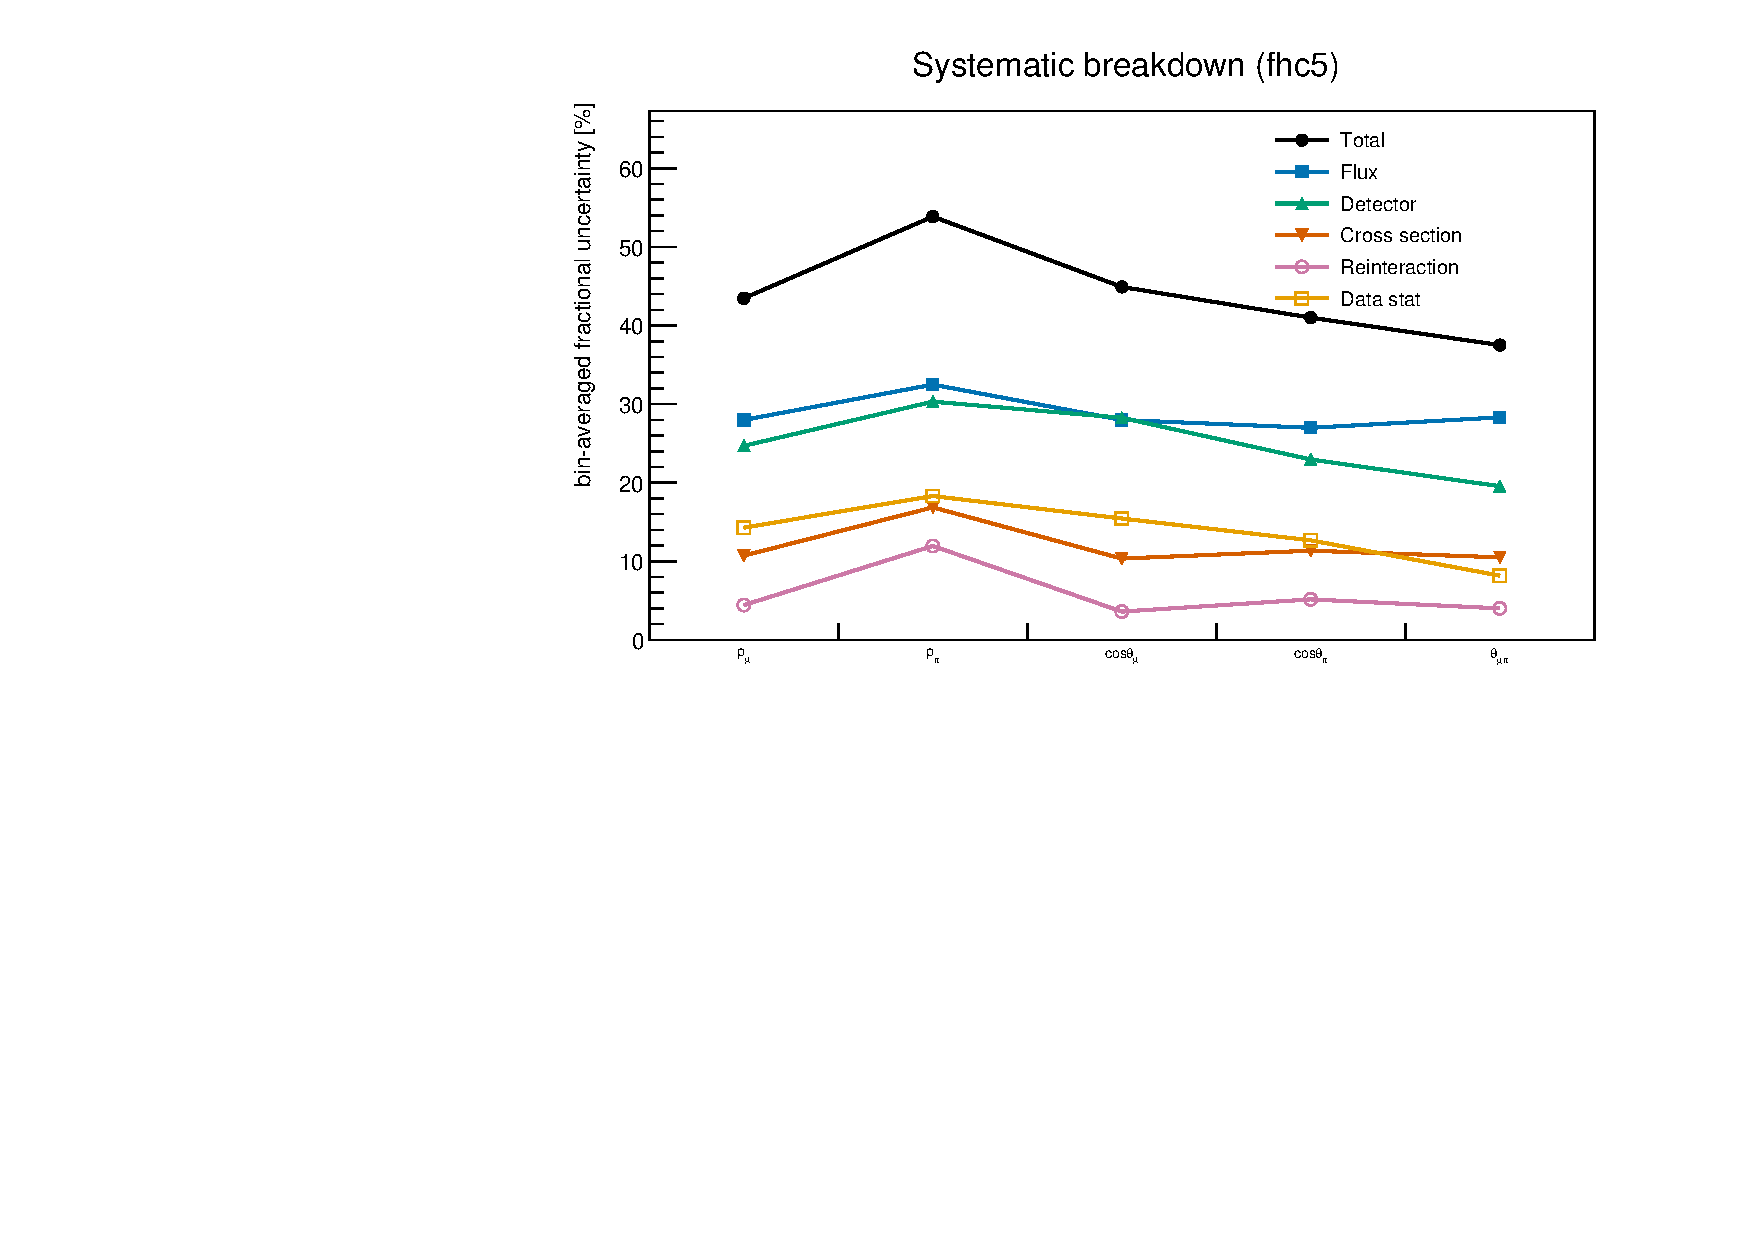
\includegraphics[width=0.32\textwidth]{fw_systbreak_fhc}\hfill
  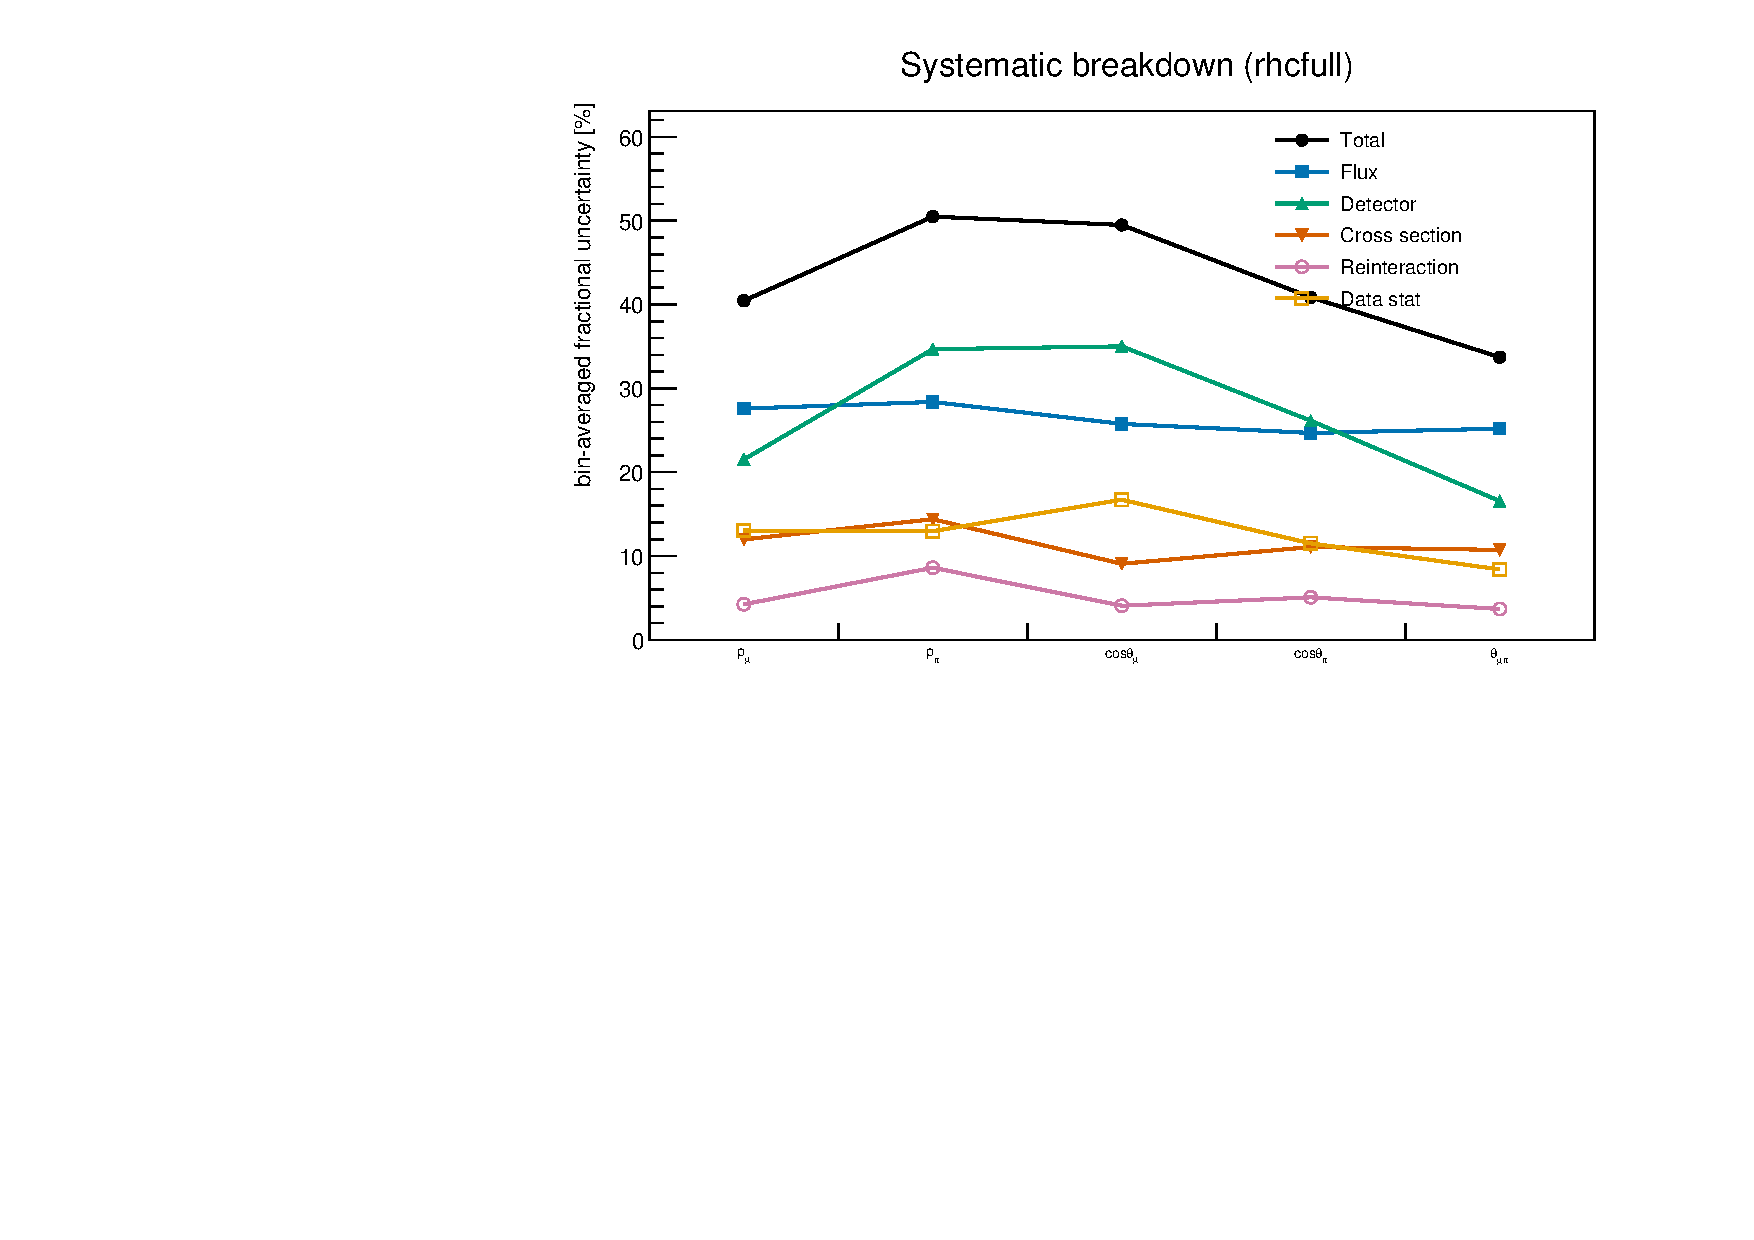
\includegraphics[width=0.32\textwidth]{fw_systbreak_rhc}\hfill
  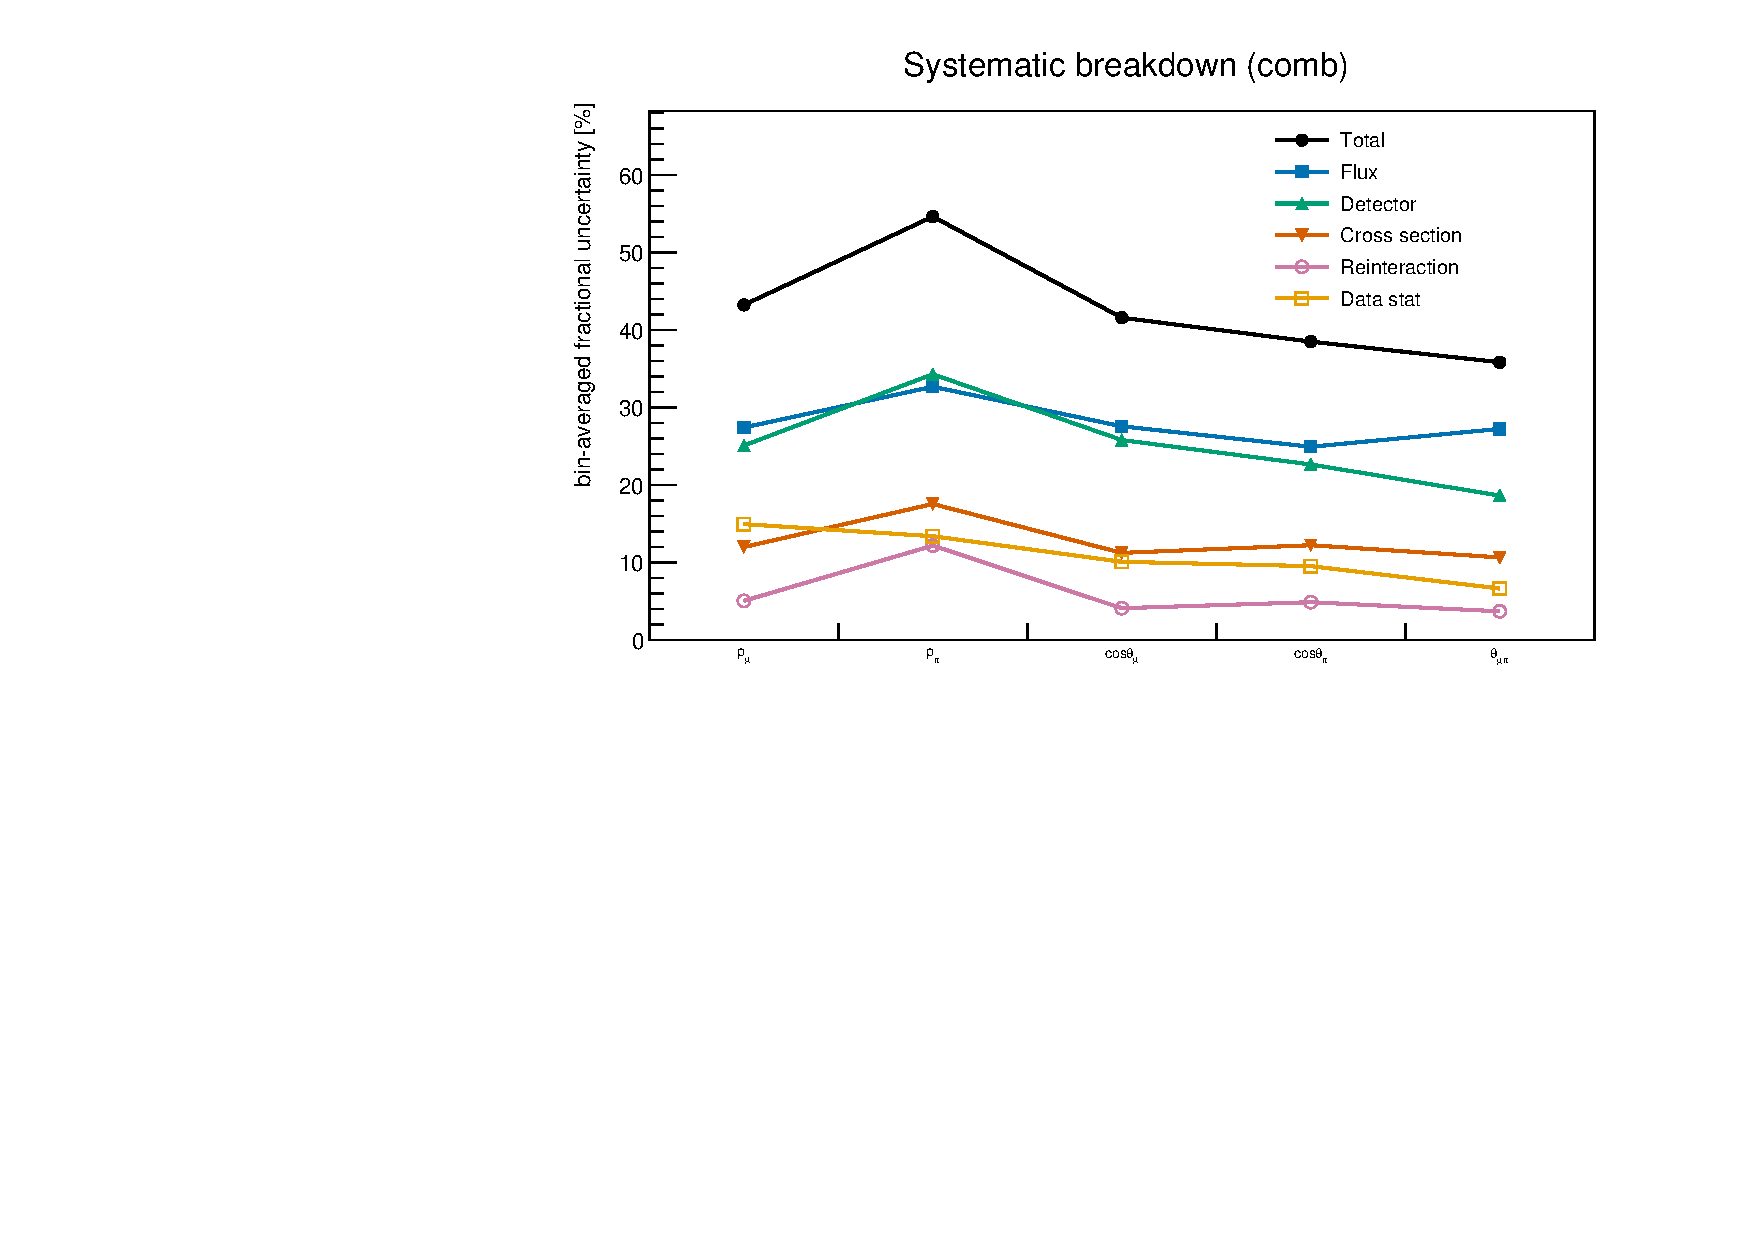
\includegraphics[width=0.32\textwidth]{fw_systbreak_comb}
  \caption{Bin-averaged fractional systematic uncertainty by source vs.\ observable,
    for FHC (left), RHC (centre) and combined (right); the figure form of
    \suppref{Table}{tab:systbreak_fhc}--\suppref{Table}{tab:systbreak_comb}. Colours use the
    Okabe-Ito colourblind-safe palette with distinct markers per source: total
    (black), flux (blue), detector (green), cross section (vermillion),
    reinteraction (purple), data stat (orange).}
  \label{fig:systbreak}
\end{figure}

\subsection{Anatomy of the flux term: why $17\%$ becomes $30\%$}
\label{sec:fluxanatomy}

\noindent\fbox{\parbox{0.97\linewidth}{\textbf{Why a $17\%$ flux uncertainty becomes
$28$--$30\%$ on the total.} A flux universe scales signal and neutrino background together,
and the extracted signal is $(N_{\rm pred}-B)/(\varepsilon\Phi N_{\rm Ar})$, so its
fractional flux variation is $\delta\Phi/\Phi\times(1+B/S)$: $17.7\%\times(1+637/943)=29.7\%$
for FHC against the one-bin value $30.25\%$. The one-bin total has no regularisation, so
this is background subtraction, not unfolding amplification. The lever is purity or a
data-driven background constraint (\S\ref{sec:sidebands}).}}
\medskip

The unfolded PPFX term is $24$--$33\%$ (Tables~\ref{tab:fhc}--\ref{tab:comb}) and the
one-bin total carries $28$--$30\%$ (Table~\ref{tab:cutcount}), against the $\sim\!17\%$
normalisation uncertainty of the NuMI flux itself. The difference is not amplification
by the unfolding operator: the one-bin total, which has no regularisation, carries it
too. The factor is the background subtraction. A flux universe scales the whole reconstructed prediction, signal and
neutrino background alike, and the framework's covariance is that of the prediction of
the measured quantity, $(N_{\rm pred}-B)/(\varepsilon\Phi N_{\rm Ar})$ with $B$ and $\Phi$
moving together in every universe; relative to the signal that is a fractional variation
of $\delta\Phi/\Phi\times(1+B/S)$, with $B$ the neutrino background (the beam-off and
dirt carry no flux weight). With $B/S=637/943$ (FHC, Table~\ref{tab:cutflow}) and a
reconstructed-level flux term of $17.7\%$ this gives $29.7\%$ against the one-bin FHC
value of $30.25\%$; RHC ($15\%\times(1+720/1015)=25.6\%$ against $27.7\%$) and the
proton-tagged FHC total ($17.7\%\times(1+338/376)=33.6\%$ against $34.9\%$, a sample
with a different purity) follow the same arithmetic. The differential flux terms of
$24$--$33\%$ are the same effect bin by bin, with the response conditioning adding a few
per cent in the worst-conditioned bins ($p_\pi$, $\cos\theta_\mu$) and nothing in the
best ($\theta_{\mu\pi}$).

Two consequences follow. First, the flux term is fully correlated between the flux
normalisation and the subtracted background, which is the correct treatment when both
come from the same flux prediction; a reader who wants the ``pure'' normalisation term
should read $17\%$, and the remainder is the flux dependence of the background model.
Second, the lever for reducing it is the purity of the selection (or a data-driven
background constraint from the control regions of \S\ref{sec:sidebands}), not the
regularisation. The reconstructed-level flux term is $16.4$--$17.7\%$ bin-averaged and
flat across observables, as expected of a normalisation term (the $600$ PPFX universes
reweight the same events, so it carries no Monte Carlo statistics); that is the $17\%$
referred to throughout.


% =============================================================================
\section{Limitations}
\label{sec:limitations}
% =============================================================================

This section states what limits the measurement as it stands. The studies behind the
scope decisions are in the technical supplement; the history of the analysis is in the
change log.

\paragraph{The analysis is blind, and that is the dominant limitation.}
No beam-on signal region has been opened.  Every ``data'' point is Poisson-thrown from the
central-value Monte Carlo, so everything demonstrated here concerns the extraction
machinery rather than nature.  In particular, no statement in this note tests the
background model against data.  At $\approx\!59\%$ purity, with proton-to-pion
misidentification the largest neutrino background, the measurement depends on that model
substantially, and fake-data closure cannot probe it: the same simulation supplies both
the pseudo-data and the background estimate.  This is the single largest untested
assumption in the analysis.

\paragraph{Pion momentum is not recoverable, and that sets the scope.}
Charged pions interact hadronically before ranging out, so the reconstructed momentum
saturates near $0.34\GeVc$ and carries little information above roughly $0.4\GeVc$.  Every
alternative estimator was tried --- golden-pion tagging, multiple Coulomb scattering,
calorimetry, multivariate regression, daughter-energy recovery, the proton-tagged
selection --- and a truth-level golden selection performs no better than the trained
classifier, which places the limit in the physics rather than the estimator.  This is why
$p_\pi$ is reported in two coarse bins and why the differential $W_{\pi p}$ shape is
withdrawn: at this exposure no binning satisfies both the migration and the statistics
requirement.

\paragraph{The extraction may carry a small negative offset.}
The ensemble of thirty-two throws on the current release puts the mean below the
reference by $0.5\%$ ($p_\mu$), $1.0\%$ (one-bin total) and $2.7\%$ ($\cos\theta_\mu$),
at $0.4$, $1.3$ and $1.9$ standard deviations of the mean, all from the same throws. It is
not significant individually, but it has the same sign everywhere and is largest in the
most regularised observable. No correction or uncertainty is assigned; a larger ensemble,
and one on RHC, would resolve it.

\paragraph{The $W_\mathrm{had}$ binning has not been edge-scanned.} The migration-level edge
scan that fixed the $p_\pi$ boundary (\suppref{Sec.}{sec:ppi_bias}) was not run for
$W_\mathrm{had}$, whose upper bins are narrower than its resolution half-width; the six-bin
$W_\mathrm{had}$ result is released with its closure and generator overlays, and its shape
should be read with that caveat until the scan is made (not gating).

\paragraph{No alternative-generator fake-data test exists for the released chain.}
Every closure in this note is a same-sample self-closure: the fake data are thrown from
the central-value tune that also supplies the response. The model dependence of the efficiency is therefore
untested where it matters most: the one-bin total (a single efficiency averaged over the
whole phase space) and the open-ended $p_\pi>0.205$~GeV/$c$ bin, inside which the
efficiency varies strongly with the true momentum. A NuWro or GiBUU fake-data pass through the released configurations is required before
the signal region is opened; it is not required for the control-region opening, which
compares reconstruction-level yields and does not involve the unfolding.

\paragraph{Coverage is demonstrated for three extractions, in one configuration.}
The pull and coverage study covers FHC $p_\mu$, $\cos\theta_\mu$ and the one-bin total.
All give widths consistent with unity, and $\cos\theta_\mu$ was chosen because its $A_C$
suppression is the most severe in the analysis, but RHC and the proton-tagged family ---
where the statistics are sparser --- have not been tested.

\paragraph{The proton-tagged results are secondary, and their model comparisons are the
weakest part.}
Their covariance is complete with respect to the configured model and their central
values current, but the exposure does not
support a differential $W_{\pi p}$ shape, and the sample has no dedicated control region
for the $\approx\!13\%$ proton mis-tag: every existing sideband applies the proton
requirement rather than inverting it, so nothing directly constrains a wrong-track proton
assignment, which is exactly what distorts the hadronic observables.

\paragraph{The TKI prescription is borrowed from the single-proton case.}
$\delta p_T$, $\delta\alpha_T$ and $\delta\phi_T$ are exact for the $\mu+(\pi p)$ system,
but $p_n$ and $W_\mathrm{had}$ use the single-nucleon residual-mass and removal-energy
assumptions of that tool with the summed hadronic system in the proton slot
(\suppref{Sec.}{sec:wtki_reco}). Data and generators are treated identically, so the comparison
is consistent, but no truth-level closure of this prescription against a
pion-production-specific definition has been made and the bias from the residual-mass
assumption is not quantified; $p_n$ should be read as a proxy.

\paragraph{No dedicated systematic covers the MCS muon momentum.}
Sixty-three per cent of the selected muons exit the detector and take their momentum from
multiple Coulomb scattering, whose scale and resolution are not varied by the eight
detector-variation knobs; the estimator enters only through the response matrix. A
data-driven MCS-versus-range comparison on contained muons is the standard way to bound
it and has not been done here. Before the signal region is opened one of three things is
required: that comparison, on contained muons in the beam-off and overlay samples; a
propagated MCS scale and resolution variation through the response; or a quantitative
argument that the existing detector variations, several of which change the MCS
estimate through the space-charge and recombination models, already cover it. The
control-region comparison does not depend on it, since it is made at reconstruction
level with the same estimator on both sides.

\paragraph{Two beam-off terms are not in the covariance.}
The released covariance carries the beam-off statistical term but no uncertainty on the
per-run gate ratios or on the use of the Run-1 beam-off sample for Run~2, which has no
sample of its own ($14\%$ of the FHC and $23\%$ of the RHC exposure). With the beam-off
at $1.9\%$ of the selected sample a $20\%$ uncertainty on either would add $0.4\%$ to
the total; they are omitted for that reason and stated here. The beamline-geometry flux
term ($1.6$--$3.3\%$) is likewise absent (\S\ref{sec:systematics}).

\paragraph{$A_C$ is not norm preserving, so two different totals exist.}
The Wiener-SVD differential result estimates $A_C x_{\rm true}$, and the row sums fall as
low as $0.050$.  Summing it over bins therefore does not give a physical total cross
section; the physical total is the one-bin extraction, quoted separately.  Two matrices
have negative row sums in their least-determined bin.

\paragraph{Actions required before unblinding.}
The prerequisites, split by the decision they gate, are the checklist of
\suppref{Sec.}{sec:request}. In brief: the four inclusive control regions are to be opened first,
under the frozen procedure of \suppref{Sec.}{sec:cr_protocol} once the conveners have ratified it;
the signal region only after any control-region discrepancy has been treated under that
procedure, the flux constants have been confirmed as PPFX-corrected central values
(\S\ref{sec:flux_status}), the real beam-on gate counts have replaced the fake-data ones
(the Run-1 beam-off sample stands in for Run~2 permanently, \S\ref{sec:mc}), and a final
clean-cache reproduction has been made; and any proton-tagged result only after the
inverted-proton-PID control region exists (\suppref{Sec.}{sec:cr_1p_scope}). Nothing has to be
switched for the beam-off treatment: the framework detects fake data by the presence of MC
truth and selects the treatment itself, and refuses a real beam-on file unless
an explicit unblinding switch is set.

The five automated guards that protect against regression --- the normalisation manifest,
the systematics/file-list coupling assertion, the staleness check, the table-consistency
check and the blinding guard --- are described in \suppref{Sec.}{sec:pipeline}.


\section{Summary}
\label{sec:summary}
% =============================================================================

We have developed a measurement of $\nu_\mu+\bar\nu_\mu$ charged-current single
charged-pion production on argon using the full \uboone{} NuMI exposure: forward horn
current ($8.857\times10^{20}$~POT), reverse horn current ($1.1082\times10^{21}$~POT), and
their combination ($1.9939\times10^{21}$~POT).

\textbf{The analysis is blind.}  No beam-on signal region has been opened.  Every ``data''
point in this note is Poisson-thrown from the central-value Monte Carlo, so the results
demonstrate that the extraction works; they are not measurements, and no statement here
about a generator is a statement about nature.

\paragraph{Measured phase space and selection.}
$|\mathrm{PDG}_\nu|=14$, charged current, true vertex in the fiducial volume, exactly one
muon and one charged pion, no neutral pions or kaons, any number of protons, with
$p_\mu>0.15\GeVc$, $p_\pi>0.175\GeVc$ and $\theta_{\mu\pi}<2.6$~rad.  The selection
reaches $\approx\!17.5\%$ efficiency at $\approx\!59\%$ purity.  Angles and transverse
observables are defined about the per-event neutrino direction, not the detector $z$ axis.

\paragraph{What is measured.}
Fifty-one differential extractions, eighteen inclusive and thirty-three proton-tagged,
across the three configurations, plus six one-bin totals.  The primary scope is the total
flux-averaged cross section, $d\sigma/dp_\mu$, the muon and pion angular cross sections,
$d\sigma/d\theta_{\mu\pi}$, and a deliberately coarse two-bin $d\sigma/dp_\pi$.
Inclusive differential total uncertainties run $32.4$--$53.9\%$, with the detector term
$15.6$--$35.0\%$ and flux the largest single contribution; the one-bin totals carry
$37.6$--$38.7\%$.

The proton-tagged subsample is secondary scope, with differential total uncertainties
$25.1$--$147.7\%$ (the largest for the six-bin combined $W_\mathrm{had}$) and one-bin
totals of $41$--$47\%$.
Its covariance is complete with respect to the configured model, but the exposure does not support a differential $W_{\pi p}$
shape at any binning, so that result is withdrawn and only the integrated proton-tagged
cross section is offered.

\paragraph{What limits the measurement.}
Charged pions interact hadronically before ranging out, so the reconstructed momentum
saturates near $0.34\GeVc$.  A survey of alternatives --- golden-pion tagging, multiple
Coulomb scattering, calorimetry, multivariate regression, daughter-energy recovery, and the
proton-tagged selection --- recovers none of it, and a truth-level golden selection performs
no better than the classifier, which places the limit in the physics rather than the
estimator.  This is what reduces $p_\pi$ to two bins and $W_{\pi p}$ to an integrated
quantity, and it is the single most consequential limitation of the analysis.

\paragraph{Validation.}
The extraction reproduces its own input: the mean closure ratio over the eighteen inclusive
extractions is $1.010$ with second-derivative regularisation.
The algebraic identity $UR=A_C$ holds to $4.4\times10^{-6}$ (\suppref{App.}{sec:identity}), which tests the unfolding
construction rather than only its behaviour on one sample.  The released $A_C$ row sums establish
that the observable-to-observable spread of the Wiener-SVD integrals is the additional
smearing rather than physics or acceptance; D'Agostini iterative unfolding, whose integral
is flat across observables, is consistent with that (it returns its prior on central-value
input, so it cannot test more).

The closure $\chi^2$ values should not be read as agreement: their $p$-values cluster near
unity because the measurement and the truth it is compared against share their systematics,
which cancel in the residual while still inflating the covariance used to judge it.

\paragraph{Reproducibility from raw inputs.}
The release is built from the processed ntuples with every cached universe deleted, in
a single pass, so no preserved intermediate exists. An independent rebuild of the same
kind, into a separate tree so that a failure could not damage the release it was
verifying, reproduced an earlier release \emph{bin by bin}, with no bin differing by
more than $10^{-9}$ in any of the fifty-one extractions; repeating that comparison on the
release to be unblinded is a prerequisite (\suppref{Sec.}{sec:pipeline}). This is a different
question from the closure and ensemble tests: those ask whether the extraction is right,
this asks whether what is published is what the code produces. The external-reproduction
check of the released $A_C$ prescription (\S\ref{sec:ac_rowsums}) belongs to the same
class: a user must be able to regenerate every published generator curve from the
released matrix, and can.

\paragraph{History.}
The analysis reached this state through a series of corrections, each recorded in the
change log with the values before and after; the automated guards of
\suppref{Sec.}{sec:pipeline} exist because of them. This note describes the analysis as it
stands and does not repeat that history.

\paragraph{Before unblinding.}
Control regions must be opened in data first, with the permitted response to any
discrepancy fixed beforehand, and a clean rebuild from empty caches must reproduce the
release. The configuration-to-systematics coupling is asserted by the framework
(\suppref{Sec.}{sec:pipeline}).  The ensemble of throws covers three FHC extractions; extending it
to RHC and to the proton-tagged family would turn the closure caveat above into a coverage
statement for every result.


% glossary.tex -- shared by the analysis note and the technical supplement.
% Plain-language definitions, in the order a reader meets the ideas, not alphabetical.
\section*{Glossary}
\addcontentsline{toc}{section}{Glossary}
\label{sec:glossary}

\begin{description}\itemsep2pt
  \item[Signal definition] The set of particles leaving the nucleus that counts as the process being
    measured, with momentum thresholds and a fiducial requirement. It is deliberately \emph{not} a
    statement about the interaction mechanism, because final-state interactions mix mechanisms and
    only the final state is observable.
  \item[Fake data / pseudo-data] A simulated dataset used in place of beam-on data while the
    analysis is blind. Here it is a Poisson throw: each simulated event is replicated a
    Poisson-distributed number of times with mean equal to its weight at data exposure, so the
    sample has the statistical fluctuations of a real dataset.
  \item[Blind] The signal region has not been looked at in beam-on data. Every plotted ``data''
    point in these documents is fake data.
  \item[Beam-on, beam-off (EXT), dirt] Beam-on data are recorded in the beam spill; beam-off data are
    recorded between spills and measure cosmic-ray activity; ``dirt'' is simulated neutrino
    interactions outside the cryostat whose products enter the detector. The prediction is
    neutrino simulation $+$ beam-off $+$ dirt.
  \item[Gate ratio] The factor scaling beam-off data to the beam-on exposure: the ratio of the number
    of beam-on to beam-off trigger gates in a running period.
  \item[Tune, central value (CV)] The \uboone{} tune is the collaboration's adjusted GENIE model; the
    central value is the nominal prediction from it. ``CV weight'' is the per-event weight that
    turns the raw simulation into the tuned prediction.
  \item[Safe-weight rule] Any event weight that is non-finite, negative or above $30$ is replaced by
    $1$. One rule, applied everywhere, so that the prediction and every pseudo-data throw agree.
  \item[Universe] One alternative version of the prediction with a systematic parameter varied. A
    \emph{multisim} is a set of hundreds of universes drawn randomly from the parameter
    uncertainties; a \emph{unisim} is a single $\pm1\sigma$ variation of one parameter. PPFX
    universes vary the flux; GENIE universes the interaction model; reinteraction universes the
    hadron transport.
  \item[Detector variations (detVar)] Dedicated simulation samples with one aspect of the detector
    response changed --- light yield, recombination, space-charge, wire response --- used to
    estimate the detector uncertainty.
  \item[Migration matrix, efficiency, smearceptance] The migration matrix $M_{ij}$ is the probability
    that an event in true bin $j$ is reconstructed in bin $i$; the efficiency $\varepsilon_j$ is the
    fraction of true bin $j$ that is selected at all. Their product $S_{ij}=\varepsilon_j M_{ij}$
    is the response the unfolding inverts; we call it the smearceptance matrix.
  \item[Migration diagonal] The fraction of events reconstructed in a bin that were truly in that
    bin (the column-normalised diagonal of $M$). A binning is accepted only if every bin's diagonal
    exceeds $0.68$.
  \item[Unfolding, Wiener-SVD] Solving for the true spectrum given the reconstructed one and the
    response. A plain inversion amplifies statistical noise; Wiener-SVD regularises it with a filter
    built from the simulation, trading a small bias for a large reduction in variance.
  \item[Additional-smearing matrix $A_C$] The price of regularisation, made explicit: the unfolded
    result estimates $A_C\,T$ rather than the truth $T$. A prediction must be multiplied by $A_C$
    before it is compared with the result. $A_C$ is released with every extraction.
  \item[Not normalisation-preserving] The rows of $A_C$ do not sum to one, so the integral of an
    unfolded differential result is not the total cross section and differs between observables of
    the same sample. The total is measured separately.
  \item[One-bin extraction] The total cross section, extracted with a single true bin covering the
    whole phase space. Nothing is regularised, $A_C=1$, and the result is the physical total.
  \item[Conditioning, $s_{\min}/s_1$, rank-deficient] The ratio of the smallest to the largest
    singular value of the regularised response. Near zero, some direction in the true spectrum
    cannot be recovered from the data at all (rank-deficient); the result in that direction is the
    prior. A binning can pass the migration-diagonal criterion and still be unusable here.
  \item[Closure] Unfolding pseudo-data and checking that the truth comes back. Closure against the
    $A_C$-smeared truth tests the implementation; it cannot test whether the model is right,
    because the same model is on both sides.
  \item[Covariance] The matrix of uncertainties and their correlations between bins, one per
    systematic source, propagated through the unfolding. ``Nominal configured covariance'' means the
    sum over the sources implemented in the analysis; the sources known to be missing are listed
    in the limitations.
  \item[Flux-averaged cross section] The cross section averaged over the neutrino energy spectrum
    of the beam, per argon nucleus, in the stated phase space. It depends on the flux, which is why
    each horn configuration is a separate measurement.
  \item[FHC, RHC] Forward and reverse horn current: the two polarities of the NuMI focusing horns,
    giving a neutrino-dominated and an antineutrino-enriched beam.
  \item[Beam frame] All angles are measured about the neutrino direction, which at \uboone{}'s
    off-axis position is $28^\circ$ from the detector $z$ axis.
  \item[Control region, sideband] A sample selected by inverting one requirement of the signal
    selection, so that it is disjoint from the signal region and enriched in one background. It
    can be inspected on beam-on data while the signal region stays blind.
  \item[Transverse kinematic imbalance (TKI)] Variables built from the momenta transverse to the
    neutrino direction of the lepton and the hadronic system: $\delta p_T$, $\delta\alpha_T$,
    $\delta\phi_T$ and the inferred nucleon momentum $p_n$. They isolate nuclear effects from the
    unknown neutrino energy.
  \item[LLR particle identification] The log-likelihood-ratio score built from track $dE/dx$ that
    separates protons from muons and pions.
  \item[Generator predictions (FTE files)] Standalone GENIE, NuWro, NEUT and GiBUU predictions,
    run with the NuMI flux and binned identically to the results, stored as histograms for the
    comparison figures.
\end{description}


\appendix

\section{Observable Binning}
\label{app:binning}

Generated directly from the released \texttt{curves\_*.tsv} files, so these are by
construction the bin edges of the published results rather than a transcription.  The
binnings are identical across the three beam configurations; the inclusive
$\cos\theta_\pi$ uses the forward-split five bins below, the proton-tagged
$\cos\theta_\pi$ four (\suppref{Sec.}{sec:binopt}).

\begin{table}[H]
  \centering
  \caption{Bin edges of every released observable, read from the data release.}
  \label{tab:binning}
  \small
  \begin{tabular}{L{3.2cm} c p{8.3cm}}
    \toprule
    Observable & Bins & Edges \\
    \midrule
    \multicolumn{3}{l}{\emph{Inclusive}}\\
    \midrule
      $p_\mu$ (GeV/$c$) & 7 & 0.15, 0.35, 0.55, 0.75, 0.95, 1.25, 1.75, 3 \\
      $p_\pi$ (GeV/$c$) & 2 & 0.175, 0.205, 1$^{*}$ \\
      $\cos\theta_\mu$ & 5 & -1, 0.45, 0.65, 0.8, 0.9, 1 \\
      $\cos\theta_\pi$ & 5 & -1, -0.1, 0.35, 0.6, 0.8, 1 \\
      $\theta_{\mu\pi}$ (rad) & 5 & 0, 0.6, 0.85, 1.3, 1.85, 2.6 \\
      $\theta_\mu$ (rad) & 5 & 0, 0.43, 0.62, 0.84, 1.17, 3.15 \\
    \midrule
    \multicolumn{3}{l}{\emph{Proton-tagged}}\\
    \midrule
      $p_\mu$ (GeV/$c$) & 7 & 0.15, 0.35, 0.55, 0.75, 0.95, 1.25, 1.75, 3 \\
      $p_\pi$ (GeV/$c$) & 2 & 0.175, 0.205, 1$^{*}$ \\
      $\cos\theta_\mu$ & 5 & -1, 0.45, 0.65, 0.8, 0.9, 1 \\
      $\cos\theta_\pi$ & 4 & -1, -0.1, 0.35, 0.75, 1 \\
      $\theta_{\mu\pi}$ (rad) & 5 & 0, 0.6, 0.85, 1.3, 1.85, 2.6 \\
      $W_{\pi p}$ (GeV/$c^2$) & 6 & 1.08, 1.19, 1.23, 1.27, 1.34, 1.47, 2.9 \\
      $W_{\rm had}$ (GeV/$c^2$) & 6 & 0, 0.78, 1.08, 1.21, 1.31, 1.44, 2.74 \\
      $\delta p_T$ (GeV/$c$) & 2 & 0, 0.3, 2.5 \\
      $\delta\phi_T$ (deg) & 2 & 0, 50, 180 \\
      $\delta\alpha_T$ (deg) & 2 & 0, 120, 180 \\
      $p_n$ (GeV/$c$) & 2 & 0, 0.375, 2 \\
      $\theta_p$ (rad)$^{\dagger}$ & 4 & 0, 0.659, 1.068, 1.539, $\pi$ \\
      $\theta_{\pi p}$ (rad)$^{\dagger}$ & 3 & 0, 1.193, 2.010, $\pi$ \\
    \bottomrule
  \end{tabular}
  \par\smallskip\noindent{\footnotesize $^{\dagger}$ Proposed secondary scope: the proton polar angle and the pion--proton
    opening angle (\S\ref{sec:wtki_ang}). $\theta_p$ uses edges derived on the RHC chain, which condition three
    times better than the FHC-derived ones at the same bin count.\par $^{*}$ Numerical plotting boundary only; the upper truth bin is open-ended ($p_\pi>0.205$~GeV/$c$), and the released density over the conventional width $0.795$~GeV/$c$ represents the bin integral (\suppref{Table}{tab:ppi_partial}).}

\end{table}

The migration-diagonal criterion itself was also relaxed, from $0.68$ to
$0.50$ admits twenty-six new candidate binnings, and \emph{every one of them} fails the secondary
gate on the conditioning of $A_C$, which is not the diagonal. The only healthy candidate is a
two-bin $W_\mathrm{had}$, and the six-bin scheme is kept, since two bins buy conditioning by
discarding the shape the observable is measured for. No binning in this note changes as a result.

Every released binning was tested for whether finer or more bins are admissible
(\suppref{Sec.}{sec:binning_recheck}): $p_\mu$, $\cos\theta_\mu$, $\theta_\mu$ and $p_\pi$
cannot go finer, $\theta_{\mu\pi}$ gains bins but no resolved information, and
$\cos\theta_\pi$ admits a fifth bin in the forward hemisphere (edges
$-1,-0.1,0.35,0.6,0.8,1$) with better-conditioned $A_C$ and unchanged per-bin
uncertainties, which is the released binning; the generator predictions are computed at
these edges from the event-level files.

The top $p_\pi$ bin is defined at truth level as $p_\pi>0.205$~GeV/$c$ with \emph{no upper edge}.
An open-ended bin has no width, so it has no differential density: the $1$~GeV/$c$ listed above is a
reporting convention that assigns the bin a finite width of $0.795$~GeV/$c$ so that it can be
plotted on the same axis as the first, and it is not a kinematic limit of the sample. A height read
off that plot is that convention, not a measured $\mathrm{d}\sigma/\mathrm{d}p_\pi$. The quantities
that are unambiguous are the two bin integrals, which is how the result should be quoted and
compared (Table~\ref{tab:ppi_partial_main}).

\section{Alternative binnings considered}
\label{app:altbinning}

Every released binning is the coarsest that satisfies the migration-diagonal criterion, and finer
schemes were tested rather than assumed unusable. The criterion itself was also relaxed, from the
$0.68$ column-normalised diagonal to $0.50$, to see what that would admit: twenty-six further
candidates pass the relaxed diagonal, and all but one fail the secondary requirement, which is the
conditioning of the additional-smearing matrix $A_C$. A binning that migrates acceptably can still
give a response that cannot be inverted, and that --- not the diagonal --- is what limits this
measurement. Table~\ref{tab:altbinning} lists the alternatives and their fate.

\begin{table}[H]
  \centering
  \caption{Alternative binnings examined. $s_{\min}/s_1$ is the conditioning of $A_C$ (FHC/RHC
    unless stated); a value near zero means the regularised response cannot be inverted, whatever
    the migration diagonal says. Only the two-bin $W_\mathrm{had}$ is healthy, and it was not
    adopted.}
  \label{tab:altbinning}
  \footnotesize
  \begin{tabular}{llcp{5.3cm}}
    \toprule
    Observable & Alternative & $s_{\min}/s_1$ & Status \\
    \midrule
    $\cos\theta_\mu$ & 6 bins & $0.11/0.09$ & not adopted: conditioning \\
                     & 7 bins & $0.02/0.05$ & not adopted: conditioning \\
    $\theta_\mu$ & 7, 8 bins & $0.00/0.00$ & not adopted: rank-deficient \\
    $p_\pi$ & 3 bins & $0.05/0.01$ & not adopted: conditioning \\
    $\delta p_T$ & 3 bins & $0.00/0.00$ & not adopted: rank-deficient \\
    $\delta\alpha_T$ & 3 bins & $0.03/0.01$ & not adopted: conditioning \\
    $W_{\pi p}$ & 2 bins & $0.26/0.15$ & sound response, no shape (App.~\ref{app:withdrawn}) \\
    $W_\mathrm{had}$ & 2 bins & $\mathbf{0.58/0.54}$ & healthy; \emph{not} adopted, six bins keep the shape \\
    $\cos\theta_p$ & 4 bins & $0.45/0.02$ & superseded by $\theta_p$ \\
                   & 6 bins & $0.00/0.00$ & not adopted: rank-deficient \\
    $\theta_p$ & 5, 7 bins & $\le0.03$ & not adopted: conditioning \\
               & 3 bins (RHC edges) & $0.16/0.05$; COMB $0.51$ & alternative to the released four bins \\
    $\cos\theta_\pi$ & 4 bins & $0.27/0.24$ & superseded by the five-bin scheme \\
    \bottomrule
  \end{tabular}
\end{table}

Two entries deserve a sentence. The two-bin $W_\mathrm{had}$ is the only candidate whose response is
healthier than the released one, and it was still not adopted: two bins buy that conditioning by
discarding almost all of the shape, and the shape is what $W_\mathrm{had}$ is measured for. The
three-bin $\theta_p$ reaches the best combined conditioning of anything tried ($0.51$), but the
released four-bin scheme is better balanced across the two configurations in which $\theta_p$ is
quoted, and keeps a bin.

\section{Withdrawn results}
\label{app:withdrawn}

Two results were extracted, examined and withdrawn. They are recorded here rather than in the body
because the reasons are properties of the response, not of the measurement being reported, and
because their files remain in the data release, where they could otherwise be mistaken for results.
\textbf{Neither is to be quoted.}

\subsection{The differential \texorpdfstring{$W_{\pi p}$}{W pi p} shape}

The directly measured pion--proton invariant mass is the observable that would show the
$\Delta(1232)$ directly, and it is the reason the proton-tagged subsample was built. At this
exposure its shape is not measurable at any binning tried. The six-bin scheme that resolves the
resonance region has a top bin only $2\%$ diagonal: essentially every event reconstructed there
comes from somewhere else. Coarsening to two bins restores the response ($s_{\min}/s_1=0.26$ FHC,
$0.15$ RHC) but leaves an observable with no shape to speak of, and the two-bin scheme was not
adopted for that reason. Closure against the $A_C$-smeared truth does not rescue the six-bin
result: closure tests whether the extraction inverted the response it was given, and cannot restore
information the response does not contain.

What the proton-tagged sample does support is the \emph{integrated} cross section, which is
released, and the calorimetric hadronic mass $W_\mathrm{had}$, whose response is sound at six bins.

\subsection{The five-bin \texorpdfstring{$d\sigma/dp_\pi$}{d sigma / d p pi}}

Charged pions interact hadronically before ranging out, so the reconstructed momentum saturates
near $0.34$~GeV/$c$ and the migration matrix loses its diagonal above it: four of the five bins
fall below the $68\%$ criterion, the top bin reaching $6\%$. The released $d\sigma/dp_\pi$ is
therefore a two-bin result --- a near-threshold interval and one broad inclusive interval --- and
is a two-region partition rather than a spectrum. The limitation is the estimator, not the binning:
range-based momentum is only valid for a pion that stops, and no rebinning of a saturated variable
recovers the information.

\section{Selection Cut Parameter Summary}
\label{app:cutparams}

\begin{table}[H]
  \centering
  \caption{All selection threshold constants.}
  \label{tab:cutparams}
  \begin{tabular}{lrl}
    \toprule
    Parameter & Value & Ntuple variable \\
    \midrule
    Topological score           & $>0.67$        & Pandora score \\
    Muon track score            & $>0.80$        & Pandora track score \\
    Muon vertex distance        & $\leq 4.0$~cm  & \\
    Muon track length           & $>10.0$~cm     & \\
    Muon LLR PID                & $>0.20$        & LLR PID \\
    Muon MIP BDT                & $\geq-0.10$    & TMVA BDT \\
    Pion track length           & $>20.0$~cm     & \\
    Pion vertex distance        & $<4.0$~cm      & \\
    Pion LLR PID                & $>0.10$        & LLR PID \\
    Pion MIP BDT                & $>-0.10$       & TMVA BDT \\
    Pion pion-BDT               & $>-0.10$       & TMVA BDT \\
    Pion Bragg score            & $\geq 0.08$    & Bragg likelihood \\
    Max.\ opening angle         & $<2.6$~rad     & \\
    Shower Y-plane hits         & $<50$ (if 1 shower) & \\
    Shower vertex distance      & $>10$~cm (if 1 shower) & \\
    Non-proton multiplicity     & $<4$           & LLR PID $>0.1$ \\
    Primary track multiplicity  & $<5$           & \\
    Cosmic BDT                  & $>0.0$ (disabled) & TMVA BDT \\
    Software trigger            & $=1$           & \\
    \midrule
    \multicolumn{3}{l}{\emph{Proton-tagged selection only (\S\ref{sec:selection_1p})}} \\
    Leading-proton LLR PID      & $<0.05$        & most proton-like non-$\mu$/$\pi$ primary \\
    Proton end point            & in FV          & \\
    Proton momentum             & $\ge0.3\GeVc$  & proton-hypothesis calorimetric KE \\
    \bottomrule
  \end{tabular}
\end{table}

% =============================================================================
\begin{thebibliography}{99}

\bibitem{numi_nue_ccpi}
  MicroBooNE Collaboration,
  ``Measurement of the flux-averaged differential $\nu_e$ CC$1\pi$ cross section
  in the NuMI beam,'' Internal Note v3.2 (2025).

\bibitem{mistry_thesis}
  K.~Mistry,
  ``First Measurement of the Flux-Averaged Differential Charged-Current
  Electron-Neutrino and Antineutrino Cross Section on Argon with the MicroBooNE
  Detector,'' PhD thesis (2021).

\bibitem{nova}
  NOvA Collaboration, M.~A.~Acero \textit{et al.},
  ``New constraints on oscillation parameters from $\nu_e$ appearance and
  $\nu_\mu$ disappearance in the NOvA experiment,''
  \textit{Phys.\ Rev.\ D} \textbf{98}, 032012 (2018).

\bibitem{t2k}
  T2K Collaboration, K.~Abe \textit{et al.},
  ``Constraint on the matter--antimatter symmetry-violating phase in neutrino
  oscillations,''
  \textit{Nature} \textbf{580}, 339--344 (2020).

\bibitem{dune}
  DUNE Collaboration, B.~Abi \textit{et al.},
  ``Deep Underground Neutrino Experiment (DUNE), Far Detector Technical Design
  Report, Volume II: DUNE Physics,'' arXiv:2002.03005 [hep-ex] (2020).

\bibitem{pandora}
  J.~S.~Marshall and M.~A.~Thomson,
  ``The Pandora Software Development Kit for Pattern Recognition,''
  \textit{Eur.\ Phys.\ J.\ C} \textbf{75}, 439 (2015).

\bibitem{wienervsd}
  W.~Tang, X.~Li, X.~Qian, H.~Wei, and C.~Zhang,
  ``Data Unfolding with Wiener-SVD Method,''
  \textit{JINST} \textbf{12}, P10002 (2017), arXiv:1705.03568 [physics.data-an].

\bibitem{ppfx}
  L.~Aliaga \textit{et al.}\ (MINERvA Collaboration),
  ``Neutrino Flux Predictions for the NuMI Beam,''
  \textit{Phys.\ Rev.\ D} \textbf{94}, 092005 (2016).

\bibitem{genie}
  C.~Andreopoulos \textit{et al.},
  ``The GENIE Neutrino Monte Carlo Generator,''
  \textit{Nucl.\ Instrum.\ Methods A} \textbf{614}, 87--104 (2010).

\bibitem{sce}
  MicroBooNE Collaboration, P.~Abratenko \textit{et al.},
  ``Measurement of space charge effects in the MicroBooNE LArTPC using cosmic
  muons,''
  \textit{JINST} \textbf{15}, P12037 (2020).

\bibitem{uboone_laser}
  MicroBooNE Collaboration, C.~Adams \textit{et al.},
  ``A Method to Determine the Electric Field of Liquid Argon Time Projection
  Chambers Using a UV Laser System and Its Application in MicroBooNE,''
  \textit{JINST} \textbf{15}, P07010 (2020).

\bibitem{uboone_pandora}
  MicroBooNE Collaboration, R.~Acciarri \textit{et al.},
  ``The Pandora multi-algorithm approach to automated pattern recognition of
  cosmic-ray muon and neutrino events in the MicroBooNE detector,''
  \textit{Eur.\ Phys.\ J.\ C} \textbf{78}, 82 (2018).

\bibitem{uboone_llr}
  MicroBooNE Collaboration, P.~Abratenko \textit{et al.},
  ``Calorimetric classification of track-like signatures in liquid argon TPCs
  using MicroBooNE data,''
  \textit{JHEP} \textbf{12}, 153 (2021).

\bibitem{uboone_mcs}
  MicroBooNE Collaboration, P.~Abratenko \textit{et al.},
  ``Determination of muon momentum in the MicroBooNE LArTPC using an improved
  model of multiple Coulomb scattering,''
  \textit{JINST} \textbf{12}, P10010 (2017).

\bibitem{uboone_detvar}
  MicroBooNE Collaboration, P.~Abratenko \textit{et al.},
  ``Novel approach for evaluating detector-related uncertainties in a LArTPC
  using MicroBooNE data,''
  \textit{Eur.\ Phys.\ J.\ C} \textbf{82}, 454 (2022).

\bibitem{uboone_tune}
  MicroBooNE Collaboration, P.~Abratenko \textit{et al.},
  ``New CC0$\pi$ GENIE model tune for MicroBooNE,''
  \textit{Phys.\ Rev.\ D} \textbf{105}, 072001 (2022), arXiv:2110.14028 [hep-ex].

\bibitem{uboone_tki}
  MicroBooNE Collaboration, P.~Abratenko \textit{et al.},
  ``First double-differential measurement of kinematic imbalance in neutrino
  interactions with the MicroBooNE detector,''
  \textit{Phys.\ Rev.\ Lett.} \textbf{131}, 101802 (2023), arXiv:2301.03700 [hep-ex].

\bibitem{xsec_analyzer}
  S.~Gardiner \textit{et al.},
  ``XSecAnalyzer: a cross-section analysis framework for MicroBooNE,''
  \url{https://github.com/uboone/xsec_analyzer} (accessed 2026).

\bibitem{numi_beam}
  P.~Adamson \textit{et al.},
  ``The NuMI Neutrino Beam,''
  \textit{Nucl.\ Instrum.\ Methods A} \textbf{806}, 279--306 (2016).

\bibitem{genie3}
  L.~Alvarez-Ruso \textit{et al.}\ (GENIE Collaboration),
  ``Recent highlights from GENIE v3,''
  \textit{Eur.\ Phys.\ J.\ ST} \textbf{230}, 4449--4467 (2021).

\bibitem{nuwro}
  T.~Golan, J.~T.~Sobczyk, and J.~\.Zmuda,
  ``NuWro: the Wroc\l{}aw Monte Carlo generator of neutrino interactions,''
  \textit{Nucl.\ Phys.\ B Proc.\ Suppl.} \textbf{229--232}, 499 (2012).

\bibitem{gibuu}
  O.~Buss \textit{et al.},
  ``Transport-theoretical description of nuclear reactions,''
  \textit{Phys.\ Rept.} \textbf{512}, 1--124 (2012);
  U.~Mosel, ``Neutrino event generators: foundation, status and future,''
  \textit{J.\ Phys.\ G} \textbf{46}, 113001 (2019).

\bibitem{neut2021}
  Y.~Hayato and L.~Pickering,
  ``The NEUT neutrino interaction simulation program library,''
  \textit{Eur.\ Phys.\ J.\ ST} \textbf{230}, 4469--4481 (2021).

\bibitem{geant4}
  S.~Agostinelli \textit{et al.}\ (GEANT4 Collaboration),
  ``GEANT4: a simulation toolkit,''
  \textit{Nucl.\ Instrum.\ Methods A} \textbf{506}, 250--303 (2003).

\bibitem{geant4reweight}
  J.~Calcutt, C.~Thorpe, K.~Mahn, and L.~Fields,
  ``Geant4Reweight: a framework for evaluating and propagating hadronic
  interaction uncertainties in Geant4,''
  \textit{JINST} \textbf{16}, P08042 (2021).

\bibitem{tmva}
  A.~Hoecker \textit{et al.},
  ``TMVA: Toolkit for Multivariate Data Analysis,''
  PoS \textbf{ACAT}, 040 (2007), arXiv:physics/0703039.

\bibitem{dagostini}
  G.~D'Agostini,
  ``A multidimensional unfolding method based on Bayes' theorem,''
  \textit{Nucl.\ Instrum.\ Methods A} \textbf{362}, 487--498 (1995).

\bibitem{lu_tki}
  X.-G.~Lu, L.~Pickering, S.~Dolan, G.~Barr, D.~Coplowe, Y.~Uchida, D.~Wark,
  M.~O.~Wascko, A.~Weber, and T.~Yuan,
  ``Measurement of nuclear effects in neutrino interactions with minimal
  dependence on neutrino energy,''
  \textit{Phys.\ Rev.\ C} \textbf{94}, 015503 (2016).

\bibitem{furmanski_pn}
  A.~P.~Furmanski and J.~T.~Sobczyk,
  ``Neutrino energy reconstruction from one-muon and one-proton events,''
  \textit{Phys.\ Rev.\ C} \textbf{95}, 065501 (2017).

\bibitem{rs_coherent}
  D.~Rein and L.~M.~Sehgal,
  ``Coherent $\pi^0$ production in neutrino reactions,''
  \textit{Nucl.\ Phys.\ B} \textbf{223}, 29--44 (1983).

\bibitem{berger_sehgal_coherent}
  C.~Berger and L.~M.~Sehgal,
  ``Partially conserved axial vector current and coherent pion production by
  low energy neutrinos,''
  \textit{Phys.\ Rev.\ D} \textbf{79}, 053003 (2009).

\bibitem{genieccpi}
  MicroBooNE Collaboration, P.~Abratenko \textit{et al.},
  ``First Measurement of Energy-Dependent Inclusive Muon-Neutrino
  Charged-Current Cross Sections on Argon with the MicroBooNE Detector,''
  \textit{Phys.\ Rev.\ Lett.} \textbf{128}, 151801 (2022), arXiv:2110.14023 [hep-ex].

\bibitem{uboone_nim}
  MicroBooNE Collaboration, R.~Acciarri \textit{et al.},
  ``Design and Construction of the MicroBooNE Detector,''
  \textit{JINST} \textbf{12}, P02017 (2017).

\bibitem{uboone_crt}
  MicroBooNE Collaboration, C.~Adams \textit{et al.},
  ``Design and construction of the MicroBooNE Cosmic Ray Tagger system,''
  \textit{JINST} \textbf{14}, P04004 (2019).

\bibitem{rs1981}
  D.~Rein and L.~M.~Sehgal,
  ``Neutrino Excitation of Baryon Resonances and Single Pion Production,''
  \textit{Ann.\ Phys.} \textbf{133}, 79--153 (1981).

\bibitem{kuzmin2004}
  K.~S.~Kuzmin, V.~V.~Lyubushkin, and V.~A.~Naumov,
  ``Lepton polarization in neutrino nucleon interactions,''
  \textit{Mod.\ Phys.\ Lett.\ A} \textbf{19}, 2815--2829 (2004).

\bibitem{graczyk2008}
  K.~M.~Graczyk and J.~T.~Sobczyk,
  ``Form factors in the quark resonance model,''
  \textit{Phys.\ Rev.\ D} \textbf{77}, 053001 (2008)
  [Erratum: \textit{Phys.\ Rev.\ D} \textbf{79}, 079903 (2009)].

\bibitem{berger2007}
  C.~Berger and L.~Sehgal,
  ``Lepton mass effects in single pion production by neutrinos,''
  \textit{Phys.\ Rev.\ D} \textbf{76}, 113004 (2007).

\bibitem{nowak2009}
  J.~A.~Nowak (MiniBooNE Collaboration),
  ``Four-momentum transfer discrepancy in the charged current $\pi^+$ production
  in the MiniBooNE: Data vs.\ theory,''
  \textit{AIP Conf.\ Proc.} \textbf{1189}, 243--248 (2009).

\bibitem{neut}
  Y.~Hayato,
  ``A neutrino interaction simulation program library NEUT,''
  \textit{Acta Phys.\ Polon.\ B} \textbf{40}, 2477--2489 (2009).

\bibitem{anl_radecky1982}
  G.~M.~Radecky \textit{et al.}\ (ANL Collaboration),
  ``Study of single pion production by weak charged currents in low-energy
  $\nu d$ interactions,''
  \textit{Phys.\ Rev.\ D} \textbf{25}, 1161--1173 (1982).

\bibitem{bnl_kitagaki1986}
  T.~Kitagaki \textit{et al.}\ (BNL Collaboration),
  ``Charged-current exclusive pion production in neutrino--deuterium
  interactions,''
  \textit{Phys.\ Rev.\ D} \textbf{34}, 2554--2565 (1986).

\bibitem{k2k_rodriguez2008}
  A.~Rodriguez \textit{et al.}\ (K2K Collaboration),
  ``Measurement of single charged pion production in the charged-current
  interactions of neutrinos in a 1.3~GeV wide band beam,''
  \textit{Phys.\ Rev.\ D} \textbf{78}, 032003 (2008).

\bibitem{miniboone_ccpi}
  A.~A.~Aguilar-Arevalo \textit{et al.}\ (MiniBooNE Collaboration),
  ``Measurement of $\nu_\mu$-induced charged-current single positive pion
  production cross sections on mineral oil at $E_\nu \in 0.5$--$2.0$~GeV,''
  \textit{Phys.\ Rev.\ D} \textbf{83}, 052007 (2011).

\bibitem{minerva_tki}
  X.-G.~Lu \textit{et al.}\ (MINERvA Collaboration),
  ``Measurement of final-state correlations in neutrino muon-proton mesonless
  production on hydrocarbon at $\langle E_\nu\rangle=3$~GeV,''
  Phys.\ Rev.\ Lett.\ \textbf{121}, 022504 (2018).

\bibitem{minerva_ccpi}
  B.~Eberly \textit{et al.}\ (MINERvA Collaboration),
  ``Charged pion production in $\nu_\mu$ interactions on hydrocarbon at
  $\langle E_\nu \rangle = 4.0$~GeV,''
  \textit{Phys.\ Rev.\ D} \textbf{92}, 092008 (2015).

\bibitem{minerva_fe}
  C.~L.~McGivern \textit{et al.}\ (MINERvA Collaboration),
  ``Cross sections for $\nu_\mu$ and $\bar{\nu}_\mu$ induced pion production on
  hydrocarbon in the few-GeV region using MINERvA,''
  \textit{Phys.\ Rev.\ D} \textbf{94}, 052005 (2016).

\bibitem{minerva_lownu}
  MINERvA Collaboration, J.~Wolcott \textit{et al.},
  ``Evidence for Quasielastic Charge Current Antineutrino Scattering Off
  Protons in Hydrocarbon at $\langle E_{\bar\nu} \rangle = 3.5$~GeV,''
  \textit{Phys.\ Rev.\ Lett.} \textbf{116}, 081802 (2016).

\bibitem{t2k_ccpip}
  K.~Abe \textit{et al.}\ (T2K Collaboration),
  ``Measurement of the muon neutrino charged-current single $\pi^+$ production
  on hydrocarbon using the T2K off-axis near detector ND280,''
  \textit{Phys.\ Rev.\ D} \textbf{101}, 012007 (2020), arXiv:1909.03936 [hep-ex].

\bibitem{argoneut_ccpi}
  R.~Acciarri \textit{et al.}\ (ArgoNEUT Collaboration),
  ``First measurement of the cross section for $\nu_\mu$ and $\bar{\nu}_\mu$
  induced single charged pion production on argon using ArgoNEUT,''
  \textit{Phys.\ Rev.\ D} \textbf{98}, 052002 (2018), arXiv:1804.10294 [hep-ex].

\bibitem{uboone_nue_ccpi}
  MicroBooNE Collaboration, P.~Abratenko \textit{et al.},
  ``First measurement of $\nu_e$ and $\bar{\nu}_e$ charged-current single
  charged-pion production differential cross sections on argon using the
  MicroBooNE detector,''
  \textit{Phys.\ Rev.\ Lett.} \textbf{135}, 061802 (2025),
  arXiv:2503.23384 [hep-ex].

\bibitem{uboone_bnb2026_ccpi}
  MicroBooNE Collaboration, P.~Abratenko \textit{et al.},
  ``Measurement of single charged pion production in charged-current
  $\nu_\mu$-Ar interactions with the MicroBooNE detector,''
  \textit{Phys.\ Rev.\ D} \textbf{113}, 032007 (2026),
  arXiv:2509.03628 [hep-ex].

\end{thebibliography}

\section{The \uboone{} detector}
\label{sec:detector}

\subsection{Operating Principle}
\label{sec:lartpc}

A liquid argon time projection chamber records three-dimensional ionisation images
of charged-particle tracks by exploiting two properties of ultra-pure liquid argon:
\begin{enumerate}[noitemsep]
  \item Ionisation electrons produced by a traversing charged particle are not
    captured by argon atoms and can drift centimetres or metres under an applied
    electric field without significant recombination, provided the purity is
    sufficient (O$_2$-equivalent $\lesssim 100$~ppt).
  \item Argon scintillates at 127~nm (vacuum ultraviolet), producing $\sim$24\,000
    photons per MeV of deposited energy, enabling nanosecond-scale timing.
\end{enumerate}
An applied electric field drifts the ionisation electrons to a set of sense-wire
planes at the anode, which record three two-dimensional projections of each track.
The third coordinate (along the drift direction) is reconstructed from the known
drift velocity and the timing of the signals relative to the beam-gate start,
combining the two-dimensional wire images into a full 3D reconstruction.

\uboone{} operated from October 2015 to July 2021 at the Fermilab Accelerator
Laboratory, collecting data in both the Booster Neutrino Beam (BNB) and, as a
parasitic experiment, the NuMI beam~\cite{numi_beam}.  It was the world's
largest operating LArTPC until the start of SBND and ICARUS data-taking.

\subsection{Active Volume and Electric Field}
\label{sec:tpc}

The \uboone{} active volume has rectangular geometry:
$256~\mathrm{cm}$ (drift, $x$) $\times$ $233~\mathrm{cm}$ (height, $y$) $\times$
$1037~\mathrm{cm}$ (beam, $z$), containing $\approx 87$~tonnes of liquid argon at
$\approx 87$~K.  The cathode is a stainless-steel plane at $x = 256$~cm held at
$-70$~kV; the anode wire planes are at $x = 0$.  The resulting 273~V/cm drift
field gives an electron drift velocity of $\approx 1.11$~mm/$\mu$s, so the
maximum drift time across the full gap is approximately 2.3~ms.

Liquid argon purity is maintained by continuous recirculation through oxygen and
water absorbers, keeping the electron lifetime well above 5~ms (corresponding to
O$_2$-equivalent contamination below $\sim$100~ppt).  At this purity level,
charge attenuation over the full 2.56~m drift is less than 10\%.

\subsection{Wire Readout and Signal Formation}
\label{sec:wires}

Three wire planes at the anode sample the drifting charge:
\begin{itemize}[noitemsep]
  \item \textbf{U plane} (first induction): 2400 wires at $+60^\circ$ from the
    vertical, 3~mm pitch.
  \item \textbf{V plane} (second induction): 2400 wires at $-60^\circ$ from the
    vertical, 3~mm pitch.
  \item \textbf{Y plane} (collection): 3456 vertical wires, 3~mm pitch.
\end{itemize}
Induction-plane wires are biased to be transparent to the drifting electrons,
producing bipolar (derivative-like) induced signals; collection-plane wires absorb
the charge and produce unipolar signals.  The combination of two stereo induction
views at $\pm60^\circ$ and a vertical collection view provides sufficient 2D
information in each plane to resolve ambiguities during 3D reconstruction.

Front-end electronics (application-specific integrated circuits, ASICs) are
mounted inside the cryostat on the wire planes and cold-multiply each channel at
$\approx 87$~K, reducing thermal noise.  The analogue signals are digitised at
16~MHz inside the cryostat by 12-bit ADCs and transmitted over $\sim$110~m of
cold cables to warm readout electronics.  The data stream is sampled into a
circular buffer; beam triggers and cosmic triggers select 4.8~ms readout windows
(corresponding to $\approx$two full drift windows) for permanent storage.

A dead-wire region at $z \in [675.1, 775.1]$~cm interrupts the collection plane
over a 100~cm span due to a shorted wire bundle.  Tracks crossing this region
have degraded hit-counting and range-based momentum estimation; the fiducial
volume (Section~\ref{sec:fv}) excludes this region.

\subsection{Photon Detection System}
\label{sec:pmt}

Thirty-two 8-inch Hamamatsu R5912-MOD photomultiplier tubes (PMTs) are installed
behind the collection-plane wire frame facing the active volume.  The PMTs detect
the 127~nm argon scintillation light via a tetraphenyl-butadiene (TPB)
wavelength-shifting coating that converts VUV photons to visible ($\sim$430~nm)
light.  The system serves two purposes in this analysis:
\begin{enumerate}[noitemsep]
  \item \textbf{Beam-gate synchronisation}: the PMT flash time identifies which
    1.6~$\mu$s NuMI spill window produced the neutrino interaction.
  \item \textbf{Flash-matching for cosmic rejection}: the Pandora reconstruction
    associates PFParticle hypotheses with the PMT flash closest in time and
    position, suppressing out-of-time cosmic-ray muons that overlap with
    beam-induced events in the long 2.3~ms drift window.
\end{enumerate}

\subsection{Calibration and Corrections}
\label{sec:calibration}

Three independent calibration inputs are used:
\begin{itemize}[noitemsep]
  \item \textbf{UV laser system}~\cite{uboone_laser}: two pulsed laser beams produce
    straight ionisation tracks at precisely known locations.  Deviations of the
    reconstructed track positions from the known trajectories are used to build
    a three-dimensional space-charge distortion map~\cite{sce}, which is applied to all
    reconstructed hits as a position correction.  Distortions reach $\sim$10~cm
    near the anode and cathode edges.
  \item \textbf{Stopping cosmic-ray muons}: the Bragg peak of cosmic muons
    stopping inside the active volume calibrates the absolute energy scale and
    the effective recombination factor as a function of local electric field and
    drift distance.  Through-going muons calibrate relative wire-by-wire gains
    and the electron lifetime.
  \item \textbf{Michel electrons}: $\mu^- \to e^-\bar{\nu}_e\nu_\mu$ decay
    products from stopped muons provide a check of the calorimetric
    reconstruction at $E_e \lesssim 55$~MeV.
\end{itemize}

\subsection{Cosmic Ray Environment and Reconstruction}
\label{sec:cosmics}

Operating at the surface with minimal overburden, \uboone{} is exposed to a
cosmic-ray muon rate of $\approx 5$~kHz through the active volume.  Each 4.8~ms
readout window contains on average $\sim$10 cosmic-ray tracks unrelated to the
beam interaction.  The 1.6~$\mu$s NuMI spill itself contains $\lesssim 0.1$
expected cosmics on average, but the drift-window pile-up is the dominant
background at early selection stages (Section~\ref{sec:selection}).

Cosmic rejection proceeds in stages:
\begin{enumerate}[noitemsep]
  \item Flash-matching (PMT timing): candidate neutrino slices must have a
    consistent optical flash within the beam window.
  \item Topological score: the Pandora-based topological neutrino score
    discriminates between neutrino-like vertex structures and
    through-going/stopping cosmic topologies.
  \item Dedicated BDT scores: the MIP and cosmic
    scores trained on track-level and event-level features further suppress
    residual cosmics that passed the topological cut.
\end{enumerate}
The CRT (Cosmic Ray Tagger) sub-detector~\cite{uboone_crt}, consisting of
scintillator panels surrounding the cryostat, provides an additional cosmic
veto but is not used as a cut in the present analysis: the CRT branches are carried
through the event processing as pass-through quantities only, they are populated only
for the CRT-era data (Runs 3--5) and zero for the pre-CRT Run-1 exposure, and a cut would
require a data/MC tagging systematic; the residual beam-off background is subtracted
instead (\S\ref{sec:mc}).

Reconstruction uses the Pandora~\cite{pandora,uboone_pandora} multi-algorithm pattern recognition
framework, which groups hits into PFParticles organised in a hierarchy with the
neutrino interaction as the top-level particle.  Track candidates are fitted with
a Kalman-filter-based track fitter to obtain momentum from track curvature
(negligible for $<$300~MeV/$c$ muons at 273~V/cm) and from range for
contained tracks.  Log-likelihood ratio particle identification (LLR PID)~\cite{uboone_llr} using
the $dE/dx$ profile along the track is the primary tool for muon/pion/proton
separation (Section~\ref{sec:selection}).

\end{document}
